\addcontentsline{toc}{section}{\hfill[\hei 五代·两宋]\hfill}
\chead{五代·两宋} % 页眉中间位置内容

\newpage~
\phantomsection %实现目录的正确跳转
\section*{\large\hei {困曹府}~\protect\footnote{根据刘曾复先生为吴小如先生说戏总讲录音底本整理。  陈超老师注:~刘曾复先生学的《困曹府》路子是程长庚弟子、三庆班沈三元的路子,沈是谭鑫培的把兄弟,因此《困曹府》的传承不是谭派。而另外一路是李顺亭的,再往下传就是贯大元。}}  
\addcontentsline{toc}{section}{\hei 困曹府}

\hangafter=1                   %2. 设置从第1⾏之后开始悬挂缩进  %}
\setlength{\parindent}{0pt}{

{\vspace{3pt}{\centerline{{[}{\hei 第一场}{]}}}\vspace{5pt}}

\setlength{\hangindent}{52pt}{曹彬\hspace{30pt}({\akai 念})跳过虎穴龙潭,({\akai 或}:~$\cdots{}\cdots{}$虎穴,)}

\setlength{\hangindent}{52pt}{赵匡胤\hspace{20pt}({\akai 念})好似凤鹤腾空。({\akai 或}:~逃出天罗地网。)}

\setlength{\hangindent}{52pt}{曹彬\hspace{30pt}仁兄请。}

\setlength{\hangindent}{52pt}{赵匡胤\hspace{20pt}请。}

\setlength{\hangindent}{52pt}{曹彬\hspace{30pt}请坐。}

\setlength{\hangindent}{52pt}{赵匡胤\hspace{20pt}有座。}\footnote{陈超老师注:~此处台上摆骑马桌。}

\setlength{\hangindent}{52pt}赵匡胤\hspace{20pt}适才关前多蒙贤弟阖家({\akai 或}:~全家)搭救,愚兄当面谢过。

\setlength{\hangindent}{52pt}{曹彬\hspace{30pt}岂敢,小弟当报前恩。}

\setlength{\hangindent}{52pt}赵匡胤\hspace{20pt}{好说。}

\setlength{\hangindent}{52pt}{曹彬\hspace{30pt}桌案现有酒食,仁兄请来压惊。}

\setlength{\hangindent}{52pt}{赵匡胤\hspace{20pt}讨扰了。}

\setlength{\hangindent}{52pt}{曹彬\hspace{30pt}仁兄请。}

\setlength{\hangindent}{52pt}{(赵匡胤\hspace{20pt}请。)}

\setlength{\hangindent}{52pt}{曹彬\hspace{30pt}【{\akai 二黄摇板}】知恩不报非君子,忘恩负义是小人。({\akai 或}:~酒不醉人人自醉,色不迷人人自迷。)}

\setlength{\hangindent}{52pt}{赵匡胤\hspace{20pt}二相公,贤弟。({\akai 或}:~贤弟,二相公。)}

\setlength{\hangindent}{52pt}{(赵匡胤\hspace{20pt}再饮几杯。)}

\setlength{\hangindent}{52pt}{赵匡胤\hspace{20pt}睡着了。}

\setlength{\hangindent}{52pt}{({\hwfs 起初更})}

\setlength{\hangindent}{52pt}{赵匡胤\hspace{20pt}唉!想俺玄郎,今晚被困曹府({\akai 或}:~夜困曹府),好不焦虑人也------}

\setlength{\hangindent}{52pt}{赵匡胤\hspace{20pt}【{\akai 二黄慢板}】有豪杰在书房心神不爽,二相公心无事睡卧一旁。无奈何推吊窗观看月亮,真乃是中秋节({\akai 或}:~真乃是中秋夜}\footnote{段公平{\scriptsize 君}建议作``中秋月''。}{),星明月朗、轮月皎皎分外风光。}

\setlength{\hangindent}{52pt}{赵匡胤\hspace{20pt}【{\akai 二黄原板}】我本是宦门后娇生惯养,闯关东、走关西自逞豪强。思爹娘、想妹弟终朝悬望,山又高、水又深阻隔两厢。洒金桥遇苗顺曾把命讲,他算我到后来南面称王。周文王坐江山全凭姜尚,保周朝八百载国祚绵长。汉光武仗云台二十八将,文邓禹、武姚期、马武子张。小秦王收下了瓦岗诸将,有罗成锁五龙图霸称强。俺玄郎逃灾祸东西游荡,孤一身({\akai 或}:~独一身)并无有架海金梁。到如今坐江山全然不想,全然不想,登九五如南柯大梦一场。恨金鸡不报晓天光未亮,谯楼上睡着了打更儿郎。恨不得抛长枪刺落了天边月亮,用金钩钩出了红日轮光。}

\setlength{\hangindent}{52pt}{({\hwfs 起二更},张氏{\hwfs 上})}

\setlength{\hangindent}{52pt}{张氏\hspace{30pt}【{\akai 二黄摇板}】轻移莲步出房门,窗外且听他人云。}

\setlength{\hangindent}{52pt}{张氏\hspace{30pt}奴家张氏,适才关前搭救恩人,不知他有何言语,待奴细听一番。}

\setlength{\hangindent}{52pt}{赵匡胤\hspace{20pt}且住,适才关前,多蒙张氏嫂嫂,叫了我一声``丈夫'',真乃难得呀难得!({\akai 或}:~多蒙张氏嫂嫂搭救,思想起来,真是难得呀难得!)}

\setlength{\hangindent}{52pt}{赵匡胤\hspace{20pt}哎------(呀)!说什么难得------倘若(是)我那贺氏妻子,叫(道旁)人一声``丈夫'',我就是这一刀------}

\setlength{\hangindent}{52pt}{张氏\hspace{30pt}唉呀!}

\setlength{\hangindent}{52pt}{赵匡胤\hspace{20pt}唉呀,醉了!(呃,)醉了!}

\setlength{\hangindent}{52pt}{赵匡胤\hspace{20pt}【{\akai 二黄散板}】窗里窗外隔窗棂,窗里说话窗外听。窗里之人吃酒醉,}

\setlength{\hangindent}{52pt}{赵匡胤\hspace{20pt}醉了哇!醉了!(呜呜呜$\cdots{}\cdots{}$({\hwfs 吐介}))}

\setlength{\hangindent}{52pt}{赵匡胤\hspace{20pt}【{\akai 二黄散板}】窗外休听醉汉云。}

\setlength{\hangindent}{52pt}{赵匡胤\hspace{20pt}呜呜呜$\cdots{}\cdots{}$(吐{\hwfs 介})}

\setlength{\hangindent}{52pt}{张氏\hspace{30pt}【{\akai 二黄散板}】听一言来吃一惊,羞得奴家脸带红。腰间解下丝鸾带,不如一命丧残生。}

\setlength{\hangindent}{52pt}{({\hwfs 起三更},华佗{\hwfs 上}}\footnote{陈超老师注:~华佗{\hwfs 抱宝剑上}。}{)}

\setlength{\hangindent}{52pt}{华佗\hspace{30pt}【{\akai 二黄摇板}】灵霄领了玉帝命,曹府搭救赤须龙。}

\setlength{\hangindent}{52pt}{华佗\hspace{30pt}({\akai 念})闷坐松林下,修道数百年。三国我为首,自称华佗仙。}

\setlength{\hangindent}{52pt}{华佗\hspace{30pt}今有赤须龙有难,奉了玉帝敕旨,下凡搭救。来此已是曹府,不免进府寻找。}

\setlength{\hangindent}{52pt}{华佗\hspace{30pt}原来星君在此,待我用起功来。}

\setlength{\hangindent}{52pt}{华佗\hspace{30pt}({\akai 念})不用急来不用愁,真龙天子百灵佑。宝剑一挥龙瘤落,丢入长江顺水流。}

\setlength{\hangindent}{52pt}{华佗\hspace{30pt}且喜大功成就,我不免趁此机会,讨一封号。}

\setlength{\hangindent}{52pt}{华佗\hspace{30pt}参见圣上。}

\setlength{\hangindent}{52pt}{赵匡胤\hspace{20pt}(呃------)何处妖道,在此摆来摆去?}

\setlength{\hangindent}{52pt}{华佗\hspace{30pt}小道三国华佗。}

\setlength{\hangindent}{52pt}{赵匡胤\hspace{20pt}前来则甚?}

\setlength{\hangindent}{52pt}{华佗\hspace{30pt}前来讨封。}

\setlength{\hangindent}{52pt}{赵匡胤\hspace{20pt}修炼多少年了?}

\setlength{\hangindent}{52pt}{华佗\hspace{30pt}千年有余。}

\setlength{\hangindent}{52pt}{赵匡胤\hspace{20pt}嗯,可算得一洞老神仙了。}

\setlength{\hangindent}{52pt}{华佗\hspace{30pt}谢主隆恩。正是:~({\akai 念})不是天子隆恩}\footnote{段公平{\scriptsize 君}建议作``天赐隆恩''。}{重,焉得一洞老神仙。}

\setlength{\hangindent}{52pt}{({\hwfs 起四更},张氏{\hwfs 魂上})}

\setlength{\hangindent}{52pt}{张氏\hspace{30pt}({\akai 念})人死如灯灭,犹如汤浇雪。若得回阳转,水底捞明月。}

\setlength{\hangindent}{52pt}{张氏\hspace{30pt}奴家张氏阴魂是也,是奴一时不明,悬梁自尽,死后方知恩人乃是当今真龙天子,不免趁此机会,前去讨一封号。}

\setlength{\hangindent}{52pt}{张氏\hspace{30pt}参见圣上。}

\setlength{\hangindent}{52pt}{赵匡胤\hspace{20pt}啊------({\akai 或}:~呃------)何处冤鬼,在此摆来摆去?}

\setlength{\hangindent}{52pt}{张氏\hspace{30pt}冤鬼张氏。}

\setlength{\hangindent}{52pt}{赵匡胤\hspace{20pt}前来则甚?}

\setlength{\hangindent}{52pt}{张氏\hspace{30pt}前来讨封。}

\setlength{\hangindent}{52pt}{赵匡胤\hspace{20pt}呃,前者({\akai 或}:~前番)路过华山,少一圣母({\akai 或}:~缺一圣母),封你以为华山圣母之位({\akai 或}:~封你为插花圣母}\footnote{段公平{\scriptsize 君}注:~汉调二黄《水西门》剧本~(``割瘤讨封''是其中{[}第十场{]})~作``插花圣母'',豫剧似乎也是这个名字。插花圣母,不供香火,插花为供。今浙江云和龙门村瓯江边有插花殿,据传有``敕封护国插花圣母娘娘''匾。})。

\setlength{\hangindent}{52pt}{赵匡胤\hspace{20pt}金童、玉女何在?}

%金童\\玉女\footnote{陈超老师注:~金童、玉女上时,金童打幡,玉女捧托盘凤冠。}\raisebox{5pt}{\hspace{30pt}有何旨意?}
\raisebox{0pt}[22pt][16pt]{\raisebox{8pt}{金童}\raisebox{-8pt}{\hspace{-22pt}{玉女}}\raisebox{0pt}{\hspace{30pt}有何旨意?\footnote{陈超老师注:~金童、玉女上时,金童打幡,玉女捧托盘凤冠。}}}

\setlength{\hangindent}{52pt}{赵匡胤\hspace{20pt}护送圣母归位去者。({\akai 或}:~护送圣母归位,去罢。)}

%金童\\玉女\raisebox{5pt}{\hspace{30pt}领法旨。}
\raisebox{0pt}[22pt][16pt]{\raisebox{8pt}{金童}\raisebox{-8pt}{\hspace{-22pt}{玉女}}\raisebox{0pt}{\hspace{30pt}领法旨。}}

\setlength{\hangindent}{52pt}{张氏\hspace{30pt}谢主隆恩。}

\vspace{3pt}{\centerline{{[}{\hei 第二场}{]}}}\vspace{5pt}

\setlength{\hangindent}{52pt}{({\hwfs 起五更},曹小姐{\hwfs 上})}

\setlength{\hangindent}{52pt}{曹小姐\hspace{20pt}({\akai 念})忙将嫂嫂事,报与兄长知。}

\setlength{\hangindent}{52pt}{曹小姐\hspace{20pt}兄长快些醒来,大事不好了!}

\setlength{\hangindent}{52pt}{曹彬\hspace{30pt}何事惊慌?}

\setlength{\hangindent}{52pt}{曹小姐\hspace{20pt}嫂嫂悬梁自尽了!}

\setlength{\hangindent}{52pt}{曹彬\hspace{30pt}哦,待我观看。}

\setlength{\hangindent}{52pt}{曹彬\hspace{30pt}唉,嫂嫂啊$\cdots{}\cdots{}$({\hwfs 哭介})}

\setlength{\hangindent}{52pt}{曹彬\hspace{30pt}兄长醒来!}

\setlength{\hangindent}{52pt}{赵匡胤\hspace{20pt}【{\akai 二黄散板}】插花圣母归了位,三国华佗讨封回。猛然睁开丹凤眼,}

\setlength{\hangindent}{52pt}{曹彬\hspace{30pt}嫂嫂哇啊$\cdots{}\cdots{}$({\hwfs 哭介})}

\setlength{\hangindent}{52pt}{赵匡胤\hspace{20pt}【{\akai 二黄摇板}】贤弟缘何两泪垂?}

\setlength{\hangindent}{52pt}{曹彬\hspace{30pt}唉呀兄长,嫂嫂悬梁自尽了哇$\cdots{}\cdots{}$({\hwfs 哭介})}

\setlength{\hangindent}{52pt}{(赵匡胤\hspace{20pt}愚兄不信。)}

\setlength{\hangindent}{52pt}{赵匡胤\hspace{20pt}今在何处?}

\setlength{\hangindent}{52pt}{曹彬\hspace{30pt}随我来!}

\setlength{\hangindent}{52pt}{赵匡胤\hspace{20pt}唉!嫂嫂啊$\cdots{}\cdots{}$({\hwfs 哭介})}

\setlength{\hangindent}{52pt}{赵匡胤\hspace{20pt}啊贤弟,不必悲泪({\akai 或}:~休得悲恸),嫂嫂成仙去了。}

\setlength{\hangindent}{52pt}{曹彬\hspace{30pt}但愿如此。}

\setlength{\hangindent}{52pt}{家人\hspace{30pt}报!}

\setlength{\hangindent}{52pt}{家人\hspace{30pt}崔龙带兵围困府门,请二老爷答话。}

\setlength{\hangindent}{52pt}{曹彬\hspace{30pt}起过。}

\setlength{\hangindent}{52pt}{曹彬\hspace{30pt}兄长暂且回避。}

\setlength{\hangindent}{52pt}{赵匡胤\hspace{20pt}是。}

\setlength{\hangindent}{52pt}{曹彬\hspace{30pt}带路。}

\setlength{\hangindent}{52pt}{曹彬\hspace{30pt}请了。崔将军有何见谕?}

\setlength{\hangindent}{52pt}{崔龙\hspace{30pt}圣上有旨:~命大人将过关人犯,带上金殿审问。}

\setlength{\hangindent}{52pt}{曹彬\hspace{30pt}将军人马暂退一箭之地,待弟将人犯戴上刑具,一同上殿交旨。}

\setlength{\hangindent}{52pt}{崔龙\hspace{30pt}大人休得迟慢,请!}

\setlength{\hangindent}{52pt}{曹彬\hspace{30pt}有请仁兄。}

\setlength{\hangindent}{52pt}{赵匡胤\hspace{20pt}贤弟何事?}

\setlength{\hangindent}{52pt}{曹彬\hspace{30pt}今有崔龙,带领人马,要将仁兄押上金殿见驾。}

\setlength{\hangindent}{52pt}{赵匡胤\hspace{20pt}就依贤弟。}

\setlength{\hangindent}{52pt}{曹彬\hspace{30pt}仁兄受屈了。}

\setlength{\hangindent}{52pt}{赵匡胤\hspace{20pt}啊贤弟,今日何日?}

\setlength{\hangindent}{52pt}{曹彬\hspace{30pt}中秋佳节。}

\setlength{\hangindent}{52pt}{赵匡胤\hspace{20pt}明日呢?}

\setlength{\hangindent}{52pt}{曹彬\hspace{30pt}乃是十六日。}

\setlength{\hangindent}{52pt}{赵匡胤\hspace{20pt}明日,就是我光棍家出头之日了。({\akai 或}:~明日中秋,就是我光棍家出头之日了。)}

\setlength{\hangindent}{52pt}{曹彬\hspace{30pt}想你这光棍家,还有什么根本不成?}

\setlength{\hangindent}{52pt}{赵匡胤\hspace{20pt}贤弟------}

\setlength{\hangindent}{52pt}{赵匡胤\hspace{20pt}【{\akai 二黄碰板}】休道我光棍家根本不讲,请台座听玄郎细说端详:~}

\setlength{\hangindent}{52pt}{赵匡胤\hspace{20pt}【{\akai 二黄原板}】家住在西罗县}\footnote{据史载,赵匡胤出生于河南洛阳夹马营。但很多地方戏曲都传说赵匡胤是``西罗县''(约在今山西洪洞县境内)。刘曾复先生有一版说戏录音中音近似``西蒙县'',可能是``西罗县''的讹误。}{双龙街上,本姓赵名匡胤字表玄郎。头辈祖名赵暠家财颇广,二辈祖名赵霸({\akai 或}:~二辈祖名赵强;~二辈祖名淮庆)四海名扬。三辈祖名赵强({\akai 或}:~三辈祖名赵霸)隋唐为将,子不言父的名四品黄堂}\footnote{``黄堂''是古代太守衙门中的正堂,可借指太守职位。  关于赵匡胤的家世,《残唐五代史演义》中称赵匡胤的祖父为赵霸,霸生弘殷,弘殷生匡胤;~据《宋史·太祖本纪》载``太祖启运立极英武睿文神德圣功至明大孝皇帝,讳匡胤,姓赵氏,涿郡人也。高祖朓,是为僖祖,仕唐历永清、文安、幽都令。朓生珽,是为顺祖,历藩镇从事,累官兼御史中丞。珽生敬,是为翼祖,历营、蓟、涿三州刺史。敬生弘殷,是为宣祖。周显德中,宣祖贵,赠敬左骁骑卫上将军$\cdots{}\cdots{}$太祖,宣祖仲子也,母杜氏。后唐天成二年,生于洛阳夹马营,赤光绕室,异香经宿不散。体有金色,三日不变。既长,容貌雄伟,器度豁如,识者知其非常人。''}{。生下了俺玄郎面带奇相,酒醉后杀御乐}\footnote{段公平{\scriptsize 君}注:~{据{[}清{]}吴}璿{《飞龙全传》,赵闹御院(勾栏),打女乐,后离家出逃。``杀御乐''一句即谓此。汉调二黄有``}悔不该将女乐满门杀坏{''。}}{惹下祸殃。二爹娘修书信四路探望,遇柴荣和郑恩关西道旁({\akai 或}:~关西路旁)。我三人尧王庙同把香上,要学那三国中刘备、关、张。董家桥打五虎弟兄各往,柴大哥到怀庆受爵封王。好一个柴子耀不把友忘,差旗牌带书信迎接玄郎。弟兄们同饮酒花亭以上,久分手又相会畅叙衷肠。一霎时({\akai 或}:~顷刻间)鱼池内陡起风浪,吓坏了王府人俱各({\akai 或}:~吓坏了王府中个个)惊慌。大哥说鱼戏水常来常往,俺玄郎见妖魔甚是张狂。左挽弓来右搭箭照妖发放({\akai 或}:~对妖撒放;~照妖撒放),谯楼上打三筹鼓角凄凉。次日里兄带我朝见皇上,郭王爷想起了梦中箭伤。顷刻间({\akai 或}:~一霎时)传旨意将我捆绑,柴大哥奏一本({\akai 或}:~保一本)刺杀刘王。悔不该({\akai 或}:~最不该)在金殿海口夸讲,不用兵不用将独下燕邦({\akai 或}:~独上燕邦)。走西门({\akai 或}:~在西门)遇见了崔龙老将,多亏你阖家搭救玄郎。昨夜晚同饮酒桌案之上({\akai 或}:~桌案以上),俺玄郎得二梦}\footnote{刘曾复先生有一版录音作``得一梦'',似误。}{牢记心旁:~头一梦见华佗三国道长,用宝剑割龙瘤丢入长江。二贤弟你不信观看左膀,}

\setlength{\hangindent}{52pt}{曹彬\hspace{30pt}【{\footnotesize 接}{\akai 二黄原板}】果然是无肉瘤毫无损伤。}

\setlength{\hangindent}{52pt}{赵匡胤\hspace{20pt}【{\akai 二黄原板}】第二梦见张氏嫂嫂形象,项带锁披着发珠泪汪洋。我封她为圣母在华山以上,}

\setlength{\hangindent}{52pt}{赵匡胤\hspace{20pt}【{\akai 二黄散板}】有金童和玉女送至山岗({\akai 或}:~送上山岗)。}

\setlength{\hangindent}{52pt}{赵匡胤\hspace{20pt}【{\akai 二黄散板}】劝贤弟在此间休要来往,搬至在怀庆府可作家乡。柴大哥是玄郎结义兄长,大小事他必然念在玄郎。天牢内二双亲劳你探望({\akai 或}:~劳你看望),说玄郎成了功即刻还乡。}

\setlength{\hangindent}{52pt}{赵匡胤\hspace{20pt}【{\akai 二黄散板}】二贤弟将手杻与我戴上,}

(\textless{}\!{\bfseries\akai 阴锣}\!\textgreater{}崔龙{\hwfs 人马两边上},{\hwfs 巡查};~赵匡胤{\hwfs 换衣}、{\hwfs 戴手杻},{\hwfs 上})

\setlength{\hangindent}{52pt}{赵匡胤\hspace{20pt}【{\akai 二黄散板}】此一番上金殿我杀一个倒海翻江。}

\setlength{\hangindent}{52pt}{赵匡胤\hspace{20pt}【{\akai 二黄散板}】施一礼辞贤弟出门观望({\akai 或}:~入门观望),见崔龙人和马个自逞强({\akai 或}:~个个逞强)。}

\setlength{\hangindent}{52pt}{赵匡胤\hspace{20pt}【{\akai 二黄散板}】真和假是与非见尔主上,俺曹仁不犯法又有何妨?}

}
   %% 困曹府
\newpage
\subsubsection{\large\hei {下河东~{\small 之}~呼延寿廷}}
\addcontentsline{toc}{subsection}{\hei 下河东~{\small 之}~呼延寿廷}

\hangafter=1                   %2. 设置从第1⾏之后开始悬挂缩进  %}
\setlength{\parindent}{0pt}{

{\vspace{3pt}{\centerline{{[}{\hei 第一场}{]}}}\vspace{5pt}}

{领旨!}

{({\akai 念})怀揣忠义胆,保主锦江山。}

{臣呼延寿廷见驾,吾皇万岁!}

{万万岁。}

{宣臣上殿,有何国事议论?}

{欧相乃是文职官员,焉能挂得武将帅印?}

{臣与欧相有打牙仇恨,此番到了河东,犹恐}\footnote{段公平{\scriptsize 君}建议作``又恐''。}{以公报私。}

{万岁作主。}

{万万岁。}

{参见元帅!}

{身为大将,焉能不晓军令?}

{一捆四十。}

{两捆八十。}

{这三卯------}

{呵呵呵呵$\cdots{}\cdots{}$({\hwfs 冷笑介})}

{也不过就是项上的人头。}

{贼呀,贼!}

{({\akai 念})身居矮檐下,怎敢不低头。}

{哎!}

\vspace{3pt}{\centerline{{[}{\hei 第二场}{]}}}\vspace{5pt}

{回府。}

{可恼!}

{今有河东打来连环战表,要我主御驾亲征。万岁命欧相挂帅,下官以为前战先行。}

{欧相奏道:~幼年习文,中年习武。({\akai 念})习就文共武,扶保帝王都。}

{好个有道明君,言道:~待等平定河东回来,与我两家解和。}

{如此有劳夫人。}

{正是:~({\akai 念})青龙背上屯军马。}

\setlength{\hangindent}{56pt}{【{\akai 二黄导板}】这几年未出征干戈宁静,}

\setlength{\hangindent}{56pt}{【{\akai 二黄散板}】玲珑铠甲挂灰尘。}

\setlength{\hangindent}{56pt}{【{\akai 二黄散板}】迈步且把二堂进,有劳夫人点雄兵。}

\setlength{\hangindent}{56pt}{【{\akai 二黄散板}】接过夫人得胜饮,背转身来谢神灵。回头再对夫人论,下官言来你试听}\footnote{段公平{\scriptsize 君}建议作``你是听''。}{:~倘若河东遭不幸,这是呼家报仇人。}

\setlength{\hangindent}{56pt}{【{\akai 二黄散板}】辞别夫人跨金镫,}

\setlength{\hangindent}{56pt}{【{\akai 二黄散板}】但愿此去奏凯回程。}

\vspace{3pt}{\centerline{{[}{\hei 第三场}{]}}}\vspace{5pt}

{参见元帅。}

{这$\cdots{}\cdots{}$披挂来迟,元帅恕罪。}

{谢元帅!}

{圣驾到!}

{在。}

{得令。}

{令出:~圣上有旨,元帅有令:~文武百官免送。人马打从德胜门}\footnote{《京剧汇编》第十六集~苏连汉~藏本作``得胜门''。}{而出,就此响炮离京。}

{\vspace{3pt}{\centerline{{[}{\hei 第四场}{]}}}\vspace{5pt}}

{前站为何不行?}

{候令!}

{启禀元帅:~前面已到河东地界。}

{在,}

{得令。}

{令出:~下面听者:~圣上有旨,元帅有令:~就在此地,择一平阳所在,靠山近水,安营扎寨。歇兵三日,再与河东鏖战呐!}

{传令已毕。}

{\vspace{3pt}{\centerline{{[}{\hei 第五场}{]}}}\vspace{5pt}}

{({\akai 念})来到河东地,昼夜费心机。}

{带马。}

{(呼延寿廷{\hwfs 从上手接枪上马},{\hwfs 左转身到上场门},{\hwfs 右手出枪亮},{\hwfs 小绕到小边台口双手托枪},{\hwfs 走到下场门扎出去跺泥右手收回来举枪亮},{\hwfs 回来到台中间右转身面向外出枪提枪花},{\hwfs 转身},{\hwfs 三个提枪花},{\hwfs 枪上右手膀子},{\hwfs 枪头向左},{\hwfs 右手在胸前平端枪},{\hwfs 左手向左伸出接枪杆},{\hwfs 跨左腿},{\hwfs 踢右腿},{\hwfs 右脚落地},{\hwfs 右手在脸前画圈拿枪杆下端},{\hwfs 向右翻身面向下场门},{\hwfs 枪交左手拿枪杆下端在左腰间平端},{\hwfs 右手画圈握拳勒马},{\hwfs 弓箭步亮住},{\hwfs 下场门下})}\footnote{{\hei 这是杨小楼晚年最常用的一个下场},不仅《下河东》、《阳平关》、《战宛城》等戏用它,《挑华车》、《霸王别姬》大铲枪下场也用它,《铁笼山》姜维与司马师,《贾家楼》唐璧与来护,一前一后,{\hwfs 提枪花},{\hwfs 并马双下场}也用它。\\{\hei 《下河东》呼延寿廷耍两个枪下场。头一个下场是呼延闻报后急于出马救欧阳芳,所以上马后只耍一个小下场表示急忙上阵。第二个下场是呼延杀败白龙太子,追击一程,用大下场。}}

{\vspace{3pt}{\centerline{{[}{\hei 第六场}{]}}}\vspace{5pt}}

{元帅受惊了,元帅受惊了!}

{你与白龙交战,堪堪落马,多亏末将一马当先,将你救下。来来来,请上功劳簿{\footnotesize 哇}。}

{这$\cdots{}\cdots{}$无有。}

{也无有。}

{谢元帅责!}

{打的------呃,不公!}

{也不是。}

{有罪不敢抬头。}

{谢元帅。}

{是是是。}

\setlength{\hangindent}{56pt}{【{\akai 二黄散板}】奸贼做事太欺情,有功不赏反加刑。}

\setlength{\hangindent}{56pt}{【{\akai 二黄散板}】人来搀我小营进,快请姑娘到此营。}

{贤妹哪里知道,老贼与白龙交战,堪堪落马,多亏愚兄将他救下。}

{有功劳不赏,反将愚兄------唉,重责。呃$\cdots{}\cdots{}$({\hwfs 哭介})}

{贤妹呀!}

\setlength{\hangindent}{56pt}{【{\akai 二黄散板}】随王驾来愿王兴,食王爵禄当报恩。军权落在奸贼手哇,得自闲来且自清。}

{\vspace{3pt}{\centerline{{[}{\hei 第七场}{]}}}\vspace{5pt}}

{臣在暗地保驾。}

}
   %% 下河东
\newpage
\phantomsection %实现目录的正确跳转
\section*{\large\hei {龙虎斗}}
\addcontentsline{toc}{section}{\hei 龙虎斗}

\hangafter=1                   %2. 设置从第1⾏之后开始悬挂缩进  %}
\setlength{\parindent}{0pt}{

\vspace{3pt}{\centerline{{[}{\hei 第一场}{]}}}\vspace{5pt}

\setlength{\hangindent}{52pt}{赵匡胤\hspace{20pt}{[}{\akai 引子}{]}龙争虎斗,这干戈,何日罢休?}

\setlength{\hangindent}{52pt}{赵匡胤\hspace{20pt}({\akai 念})蛟龙无水困沙滩,失却明珠寻找难。奸贼诓孤河东地,不知何日返中原。}

\setlength{\hangindent}{52pt}{赵匡胤\hspace{20pt}孤,乾德王赵。可恨奸贼欧阳芳将孤诓下河东,一困七载。内无粮草,外无救应。飞报报道:~阵前来了一哨人马,杏黄旌旗招展,不知哪路救应。也曾命黄信打探,未见回报。}

\setlength{\hangindent}{52pt}{黄信\hspace{30pt}({\akai 内})马来!}

\setlength{\hangindent}{52pt}{黄信\hspace{30pt}({\akai 念})打探军情事,奏与万岁知}\footnote{刘曾复先生钞本作``报与万岁知''。}{。}

\setlength{\hangindent}{52pt}{黄信\hspace{30pt}报,黄信告进。}

\setlength{\hangindent}{52pt}{黄信\hspace{30pt}参见万岁。}

\setlength{\hangindent}{52pt}{赵匡胤\hspace{20pt}罢了!}

\setlength{\hangindent}{52pt}黄信\hspace{30pt}谢万岁。

\setlength{\hangindent}{52pt}{赵匡胤\hspace{20pt}打探军情,有何消息?。}

\setlength{\hangindent}{52pt}{黄信\hspace{30pt}臣探得军情,乃是落伽山发来人马,昨日阵前鞭诛白龙,今日马踏御营,要万岁出马,不知是何缘故,特来启奏。}

\setlength{\hangindent}{52pt}{赵匡胤\hspace{20pt}赐你金牌一面,再去打探!}

\setlength{\hangindent}{52pt}{黄信\hspace{30pt}领旨。}

\setlength{\hangindent}{52pt}{赵匡胤\hspace{20pt}且住,适才黄信报道:~落伽山发来一哨人马,昨日阵前鞭诛白龙,今日马踏御营。要孤王出马,此事叫孤难猜难解也!}

\setlength{\hangindent}{52pt}{赵匡胤\hspace{20pt}【{\akai 唢呐二黄原板}】探马儿不住地飞来报,他报道落伽山兵马一标。杏黄旗不住地\footnote{刘曾复先生钞本作``不住得''。}空中飘绕,吓坏了满营中大小儿曹。(恨河东打来了连环战表,他要夺孤王我锦绣龙朝。\footnote{刘曾复先生钞本中有此二句。})欧阳芳在金殿帅印挂了,呼延(寿)廷倒作了马前英豪。下河东连七载须发苍了,(须发苍了,)为国家哪顾得昼夜辛劳。在头上摘下了飞龙帽罩,}

\setlength{\hangindent}{52pt}{赵匡胤\hspace{20pt}【{\akai 唢呐二黄原板}】(身上------)在身上脱下了衮龙袍。}

\setlength{\hangindent}{52pt}{赵匡胤\hspace{20pt}【{\akai 唢呐二黄散板}】孤的玲珑------玲珑铠甲丝绦绕,杀人妙计有千条。御林军且回避黄罗道\footnote{``{御林军且回避黄罗道}''  一句,陈超老师从刘曾复先生学的是``{御林军且退宝帐道}''。刘曾复先生钞本亦作``御林军且退宝帐道''。},站立辕门喊喝高。教槽头将孤的龙驹马鞍韂备好,}

\setlength{\hangindent}{52pt}{马童\hspace{30pt}啊!}

\setlength{\hangindent}{52pt}{马童\hspace{30pt}请万岁上马!}

\setlength{\hangindent}{52pt}{赵匡胤\hspace{20pt}【{\akai 唢呐二黄散板}】这才是无良将亲把兵交。}

\vspace{3pt}{\centerline{{[}{\hei 第二场}{]}}}\vspace{5pt}

\setlength{\hangindent}{52pt}{呼延赞\hspace{20pt}哈哈,哈哈,哇呀呀$\cdots{}\cdots{}$({\hwfs 笑介})}

\vspace{3pt}{\centerline{{[}{\hei 第三场}{]}}}\vspace{5pt}

\setlength{\hangindent}{52pt}{赵匡胤\hspace{20pt}【{\akai 唢呐二黄摇板}】催马来在战场道,看一看落伽山哪家英豪。}

\setlength{\hangindent}{52pt}{呼延赞\hspace{20pt}({\akai 内})【{\akai 唢呐二黄导板}】乌骓马不住得连声吼,}

\setlength{\hangindent}{52pt}{呼延赞\hspace{20pt}【{\akai 唢呐二黄原板}】打将鞭一举鬼神愁。催战马来至在双阳道口,}

\setlength{\hangindent}{52pt}{呼延赞\hspace{20pt}呔!}

\setlength{\hangindent}{52pt}{呼延赞\hspace{20pt}【{\akai 唢呐二黄原板}】叫一声乾德王快出龙楼。}

\setlength{\hangindent}{52pt}{赵匡胤\hspace{20pt}【{\akai 唢呐二黄原板}】只见他乌油盔乌油甲,}

\setlength{\hangindent}{52pt}{赵匡胤\hspace{20pt}皂罗------}

\setlength{\hangindent}{52pt}{赵匡胤\hspace{20pt}【{\akai 唢呐二黄原板}】皂罗袍上绣团花。问一声小将名和姓,通上名来哪里有家。}

\setlength{\hangindent}{52pt}{呼延赞\hspace{20pt}【{\akai 唢呐二黄原板}】家住在落伽山呼家寨,我的父就是呼延寿廷。若问少爷名和姓,}

\setlength{\hangindent}{52pt}{呼延赞\hspace{20pt}呼延赞------}

\setlength{\hangindent}{52pt}{呼延赞\hspace{20pt}【{\akai 二黄原板}】就是少爷名。}

\setlength{\hangindent}{52pt}{赵匡胤\hspace{20pt}【{\akai 二黄散板}】人道呼家无有后,哪里又来这条根。不通姓名催马走,}

\setlength{\hangindent}{52pt}{呼延赞\hspace{20pt}哪里走!}

\setlength{\hangindent}{52pt}{呼延赞\hspace{20pt}【{\akai 二黄散板}】你少爷不打无名人。}

\setlength{\hangindent}{52pt}{赵匡胤\hspace{20pt}【{\akai 二黄散板}】乾德王御驾宝帐坐,我是帐前一小军。}

\setlength{\hangindent}{52pt}{呼延赞\hspace{20pt}住口!}

\setlength{\hangindent}{52pt}{呼延赞\hspace{20pt}【{\akai 二黄散板}】蚕眉凤目龙颜相,五绺长髯飘胸膛。看你不像小军样,定是当今乾德王。}

\setlength{\hangindent}{52pt}{赵匡胤\hspace{20pt}【{\akai 二黄散板}】听一言来心火上,孤王何惧小儿郎。若问老爷名和姓呐,少打关西赵玄郎。}

\setlength{\hangindent}{52pt}{呼延赞\hspace{20pt}啊?!}

\setlength{\hangindent}{52pt}{呼延赞\hspace{20pt}【{\akai 二黄散板}】听说来了贼昏王,太阳头上冒火光。手持钢鞭朝下打呀。\textless{}\!{\bfseries\akai 扫一句}\!\textgreater{}}

\setlength{\hangindent}{52pt}{赵匡胤\hspace{20pt}【{\akai 二黄散板}】小将生来实可夸,手执钢鞭似铁塔。一鞭打下难招架,震得孤王虎口麻。勒住丝缰且住马,小将到来顺说他。}

\setlength{\hangindent}{52pt}{呼延赞\hspace{20pt}【{\akai 二黄散板}】昏王休得来逃遁,快将诡计来说清:~我父身犯何条令,缘何}\footnote{刘曾复先生钞本作``{为何''。}}{斩首在辕门。}

\setlength{\hangindent}{52pt}{赵匡胤\hspace{20pt}小将!}

\setlength{\hangindent}{52pt}{赵匡胤\hspace{20pt}【{\akai 二黄原板}】小将不必问详情,孤王言来听分明。误中奸贼反间计,满营喊叫反了那呼延寿廷。孤王我斩字未开口,}

\setlength{\hangindent}{52pt}{赵匡胤\hspace{20pt}欧阳芳,}

\setlength{\hangindent}{52pt}{赵匡胤\hspace{20pt}【{\akai 二黄原板}】欧阳芳拔剑杀尔天伦。}

\setlength{\hangindent}{52pt}{呼延赞\hspace{20pt}呸!}

\setlength{\hangindent}{52pt}{呼延赞\hspace{20pt}【{\akai 二黄散板}】你不传旨谁敢斩,哪有臣子乱杀人。}

\setlength{\hangindent}{52pt}{赵匡胤\hspace{20pt}【{\akai 二黄散板}】军权落在奸贼手,孤王也要听令行。}

\setlength{\hangindent}{52pt}{呼延赞\hspace{20pt}【{\akai 二黄散板}】懦弱之人怎为君,苍天再降紫微星。}

\setlength{\hangindent}{52pt}{赵匡胤\hspace{20pt}【{\akai 二黄散板}】小将休得胡言讲,孤王言来听端详。你若马前来归降,}

\setlength{\hangindent}{52pt}{赵匡胤\hspace{20pt}封你为前殿王。}

\setlength{\hangindent}{52pt}{呼延赞\hspace{20pt}不要!}

\setlength{\hangindent}{52pt}{赵匡胤\hspace{20pt}后殿王。}

\setlength{\hangindent}{52pt}{呼延赞\hspace{20pt}不要!}

\setlength{\hangindent}{52pt}{赵匡胤\hspace{20pt}【{\akai 二黄散板}】一十八家总兵王。}

\setlength{\hangindent}{52pt}{呼延赞\hspace{20pt}【{\akai 二黄散板}】不做官来不受管,一心要报我父冤。}

\setlength{\hangindent}{52pt}{赵匡胤\hspace{20pt}【{\akai 二黄散板}】小将说话太张狂}\footnote{刘曾复先生钞本作``{太猖狂}''。}{,不由孤王怒满膛}\footnote{刘曾复先生钞本作``怒满腔''。}{。我今与你分上下。\textless{}\!{\bfseries\akai 扫一句}\!\textgreater{}}

\vspace{3pt}{\centerline{{[}{\hei 第四场}{]}}}\vspace{5pt}

\setlength{\hangindent}{52pt}{赵匡胤\hspace{20pt}【{\akai 二黄散板}】人困马乏难交战,}

\setlength{\hangindent}{52pt}{赵匡胤\hspace{20pt}啊?!}

\setlength{\hangindent}{52pt}{赵匡胤\hspace{20pt}【{\akai 二黄散板}】只见黑虎落雕鞍}\footnote{刘曾复先生钞本作``卧雕鞍``。}{。手执金锏朝下打,}

\setlength{\hangindent}{52pt}{赵匡胤\hspace{20pt}【{\akai 二黄散板}】只见黑虎奔南山。}

\setlength{\hangindent}{52pt}{呼延赞\hspace{20pt}【{\akai 二黄散板}】梦里只见我父到,}

\setlength{\hangindent}{52pt}{呼延赞\hspace{20pt}【{\akai 二黄散板}】只见青龙卧鞍鞒。手执钢鞭朝下打,只见青龙上九霄。}

\setlength{\hangindent}{52pt}{呼延赞\hspace{20pt}哈哈,哈哈,啊哈哈哈$\cdots{}\cdots{}$({\hwfs 笑介})}

\setlength{\hangindent}{52pt}{呼延赞\hspace{20pt}【{\akai 二黄散板}】翻身下了乌骓马,}

\setlength{\hangindent}{52pt}{呼延赞\hspace{20pt}【{\akai 二黄散板}】三呼万岁把臣饶。}

\setlength{\hangindent}{52pt}{赵匡胤\hspace{20pt}【{\akai 西皮导板}】耳边厢又听得山呼万岁,}

\setlength{\hangindent}{52pt}{呼延赞\hspace{20pt}万岁!}

\setlength{\hangindent}{52pt}{赵匡胤\hspace{20pt}【{\akai 西皮原板}】是何方保驾臣来在军前。乾德王睁开了丹凤眼,只见小将【{\footnotesize 转}{\akai 西皮快板}】跌跪马前。马上擒王擒不住,诓孤下马难上难。}

\setlength{\hangindent}{52pt}{呼延赞\hspace{20pt}【{\akai 西皮快板}】万岁不必心惊怕,为臣保你坐中华。}

\setlength{\hangindent}{52pt}{赵匡胤\hspace{20pt}【{\akai 西皮快板}】你若保孤坐中华,可对苍天把誓发。}

\setlength{\hangindent}{52pt}{呼延赞\hspace{20pt}【{\akai 西皮快板}】跪在阵前把誓发,日月三光照某家。呼延赞保主若有假,死在千军万马踏。}

\setlength{\hangindent}{52pt}{赵匡胤\hspace{20pt}【{\akai 西皮快板}】一见小将把誓发,不由孤王笑哈哈。左思右想不下马,}

\setlength{\hangindent}{52pt}{赵匡胤\hspace{20pt}【{\akai 西皮散板}】金锏挑起小卿家。}

\setlength{\hangindent}{52pt}{呼延赞\hspace{20pt}【{\akai 西皮散板}】叩罢头来谢王恩,尊声万岁听分明:~我父仇人哪一个?}

\setlength{\hangindent}{52pt}{赵匡胤\hspace{20pt}【{\akai 西皮散板}】欧阳芳是尔对头人。}

\setlength{\hangindent}{52pt}{呼延赞\hspace{20pt}【{\akai 西皮散板}】老贼何处把身隐,}

\setlength{\hangindent}{52pt}{赵匡胤\hspace{20pt}【{\akai 西皮散板}】卿家后营去找寻。}

\setlength{\hangindent}{52pt}{呼延赞\hspace{20pt}【{\akai 西皮散板}】辞别万岁后营进。\textless{}\!{\bfseries\akai 扫一句}\!\textgreater{}}

\setlength{\hangindent}{52pt}{赵匡胤\hspace{20pt}【{\akai 西皮快板}】喜孜孜来笑盈盈,看来孤王有福分。今日收了这员将,}

\setlength{\hangindent}{52pt}{赵匡胤\hspace{20pt}【{\akai 西皮摇板}】哪怕河东百万兵。}

}
   %% 龙虎斗
\newpage
\subsubsection{\large\hei {贺后骂殿~{\small 之}~赵光义}}
\addcontentsline{toc}{subsection}{\hei 贺后骂殿~{\small 之}~赵光义}

\hangafter=1                   %2. 设置从第1⾏之后开始悬挂缩进  %}
\setlength{\parindent}{0pt}{

{{[}{\akai 引子}{]}兄亡侄幼,众文武,辅孤登极\footnote{``登极'',《京剧汇编》第一百零九集作``登基'',下同。}。}

{众卿平身。}

{({\akai 念})兄王晏驾龙归西,全凭争先一着棋。满朝文武来辅助,孤王才得立帝基。}

{孤,赵光义。今日登殿受贺,众卿!}

{(众\hspace{40pt}万岁!)}

{孤王登极,不知当降何国号?}

{依卿所奏。}

{代孤传旨\footnote{段公平{\scriptsize 君}建议作``待孤传旨''。},晓谕天下。}

{潘洪听封。}

{封你左班丞相,卿女执掌昭阳正院。}

{赵普听封。}

{封你右班丞相,代孤执掌朝政。}

{曹彬听封。}

{封卿孝义侯之位,代管禁军。}

{苗宗善听封。}

{封你护国军师,子袭父职。}

{潘疆\footnote{《京剧汇编》第一百零九集作``潘强''。}、潘豹。}

{封你二人为镇殿将军。}

{满朝文武,加升三级,大赦天下。}

{有本早奏,无本退班!}

{代孤传旨,宣杨继业上殿!}

{嗯------大胆杨继业,孤王登极,为何不来朝贺?}

{哪里是参驾来迟,分明藐视寡人。看孤登极,心中不服。}

{殿前武士。}

{推出斩了}

{呃------怎么参本是你,保本也是你?}

{依卿所奏。}

{将杨继业赦回!}

{非是孤王不斩于你,念你在朝有十大汗马功劳。今将你削职为民,赐你百亩田园;~无事不准入朝,限三日出京,三日不走,其罪还在。下殿!}

{\setlength{\hangindent}{56pt}{(赵德昭\hspace{20pt}【{\akai 二黄散板}】$\cdots{}\cdots{}$还我锦家邦。)} }

\setlength{\hangindent}{56pt}{【{\akai 二黄散板}】大皇儿来在金殿上,口口声声要家邦。}孤本当下位将国\textless{}\!{\bfseries\akai 哭头}\!\textgreater{}让,

\setlength{\hangindent}{56pt}{【{\akai 二黄散板}】}难学尧、舜------禹、商汤\footnote{《京剧汇编》第一百零九集作``难学尧舜与商汤''。}。

\setlength{\hangindent}{56pt}{【{\akai 二黄散板}】皇儿近前听叔讲,你母子宫中乐安康。}

{\setlength{\hangindent}{56pt}{(赵德昭\hspace{20pt}【{\akai 二黄散板}】$\cdots{}\cdots{}$你今不把江山让,篡位的名儿天下扬。)} }

{诶------}

\setlength{\hangindent}{56pt}{【{\akai 二黄散板}】皇儿休得多言讲,孤不封你自为王。吩咐潘豹与潘疆,}

%$\bigg( \begin{aligned} &\mbox{潘豹}\\&\mbox{潘疆}\mbox{\raisebox{5pt}{\hspace{28pt}有。}} \end{aligned}\bigg)$
\raisebox{0pt}[22pt][16pt]{\bigg(\raisebox{8pt}{潘豹}\raisebox{-8pt}{\hspace{-22pt}{潘疆}}\raisebox{0pt}{\hspace{22pt}有。}\bigg)}

\setlength{\hangindent}{56pt}{【{\akai 二黄散板}】再有人胡言绑云阳}\footnote{云阳,在今约陕西淳化县西北,是秦代监狱、刑场所在地。所以后常以``云阳''或``云阳市曹''{代指刑场。}}{。}

{(赵德昭\hspace{20pt}唉呀!)}

\setlength{\hangindent}{56pt}{【{\akai 二黄慢板}】自盘古立帝基天子为重\footnote{《京剧丛刊》第三十四集~贯大元~口述本作``自盘古立帝邦天子为重'';~《京剧汇编》第一百零九集作``自盘古开天地皇帝为重''。此处``立帝基''也有以盘古开天劈地故事,作``立地基''的。},老皇嫂骂孤王情理难容。论国法该将你残生断送,}

{(贺后\hspace{30pt}谁敢?!)}

{退班!}

{皇嫂!}

\setlength{\hangindent}{56pt}{【{\akai 二黄碰板三眼}】还念你与皇兄掌印正宫。先王爷晏了驾钟鼓齐动,满朝中文武臣议论孤穷\footnote{《京剧丛刊》第三十四集~贯大元~口述本作``议论皆同'';~《京剧汇编》第一百零九集作``议论不同''。}。全都道大皇儿年轻无用,一个个辅保孤驾坐九重啊。孤虽然掌山河依然大宋,并非是外姓人来坐金龙。走向前、再打一躬把皇嫂尊奉,昭阳院改作了养老宫。将皇嫂当作了太后侍奉,崇上徽号容是不容。}

\setlength{\hangindent}{56pt}{【{\akai 二黄原板}】老皇嫂说什么务农耕种,普天下尽都是老王荣封。享荣华、受富贵母子同共,并非是叔为君、侄为臣各自西东。赐皇嫂尚方剑泰山压重}\footnote{{《京剧汇编》第一百零九集作``泰山压众''。}}{,管三宫和六院,大小嫔妃若有违抗任你施行,你从也不从?}

\setlength{\hangindent}{56pt}{【{\akai 二黄原板}】赵德芳我的儿莫要悲痛,近前来听为叔将儿来封:~孤赐你金镶白玉锁,加封你一钦王、二良王、三忠、四正、五德王、六靖王,\footnote{《京剧汇编》第一百零九集作``一秦王、二梁王、三忠王、四正王、五德王、六延王,''。}上殿不参王、你下殿不辞王,再赐你凹面金锏上打昏君、下打谗臣,压定了满朝的文武,哪一个不尊,你是个八贤王,带管孤穷\footnote{《京剧丛刊》第三十四集~贯大元~口述本作``孤躬''。\\另,从吴同宾先生学戏的人曾撰文\upcite{Zhen_Jinwan}回忆,吴同宾先生亦指出,《贺后骂殿》中的``孤穷''(或``孤穹'')系讹误,当作``孤躬''(因为``躬''与``窮''字相似,旧时艺人误识,乃至因袭)。}。}

\setlength{\hangindent}{56pt}{【{\akai 二黄散板}】贤皇侄从今后莫要悲痛,老皇嫂请回养老宫。}

{\setlength{\hangindent}{56pt}{(贺后\hspace{30pt}【{\akai 二黄散板}】$\cdots{}\cdots{}$三尺龙泉不容留。)} }

{众卿!}

{孤身不爽,是何缘故?}

{(潘洪\hspace{30pt}$\cdots{}\cdots{}$休养。)}

{就命卿家,代孤办理。}

{(潘洪\hspace{30pt}领旨。)}

{退班。}

{(潘洪\hspace{30pt}$\cdots{}\cdots{}$回宫。)}
   %% 贺后骂殿
\newpage
\phantomsection %实现目录的正确跳转
\section*{\large\hei {金沙滩~{\small 之}~杨继业}}
\addcontentsline{toc}{section}{\hei 金沙滩~{\small 之}~杨继业}

\hangafter=1                   %2. 设置从第1⾏之后开始悬挂缩进  %}
\setlength{\parindent}{0pt}{

\vspace{3pt}{\centerline{{[}{\hei 第一场}{]}}}\vspace{5pt}

{({\akai 念})腰悬三尺剑,保主锦江山。}

{老夫,杨继业。宋王驾前为臣,奉主之命,巡营瞭哨。今有北国鞑儿韩昌,兴兵前来,请我主敌楼答话。众儿郎,}

{回营交旨。}

\vspace{3pt}{\centerline{{[}{\hei 第二场}{]}}}\vspace{5pt}

{({\akai 念})忙将韩昌事,奏与万岁知。}

{臣,继业见驾,吾皇万岁,}

{万万岁。}

{贤爷千岁,}

{千千岁。}

{谢座。}

{今有北国鞑儿韩昌,兴兵前来,请我主敌楼答话。}

{领旨。}

\vspace{3pt}{\centerline{{[}{\hei 第三场}{]}}}\vspace{5pt}

{(韩昌\hspace{30pt}$\cdots{}\cdots{}$宋王请了。)}

{贤爷在此!}

{(韩昌\hspace{30pt}$\cdots{}\cdots{}$巴特鲁}\footnote{``{巴特鲁}'',系满语``勇士''之意。}{。)}

{住口!}

{\textless{}{\!\bfseries\akai 三叫头}\!\textgreater{}万岁!~吾主!~唉,万岁{\footnotesize 呃}!}

\setlength{\hangindent}{56pt}{【{\akai 西皮导板}】事到如今恨奸党,}

\setlength{\hangindent}{56pt}{【{\akai 西皮原板}】潘仁美诓圣驾来到番邦。哪里是双龙会把宴上\footnote{夏行涛{\scriptsize 君}建议作``把宴赏''。},明明是一座杀人战场。若要想救主爷出罗网,除非是学纪信替主荥阳。}

\setlength{\hangindent}{56pt}{【{\akai 西皮摇板}】低下头来暗思想,}

{有了!}

\setlength{\hangindent}{56pt}{【{\akai 西皮快板}】忽然一计上心旁。继业撩铠出宝帐,}

\setlength{\hangindent}{56pt}{【{\akai 西皮快板}】众家儿郎听端详:~哪个孩儿有胆量,替主赴会到番邦。}

\setlength{\hangindent}{56pt}{【{\akai 西皮摇板}】答话儿郎哪一个,}

\setlength{\hangindent}{56pt}{【{\akai 西皮摇板}】进帐来父子们再作商量。}

{儿有此胆量?}

{好哇!}

\setlength{\hangindent}{56pt}{【{\akai 西皮散板}】这才是父是英雄儿有胆量,杨家出了假宋王。}

\setlength{\hangindent}{56pt}{【{\akai 西皮散板}】父子一同进宝帐,}

\setlength{\hangindent}{56pt}{【{\akai 西皮散板}】把本启奏圣吾皇。}

{臣启万岁:~长子延平愿替主赴会。}

{看衣更换。}

{儿啊!}

\setlength{\hangindent}{56pt}{【{\akai 西皮快板}】我的儿休得悲声放,痛哭尤恐惊君王。继业二次出宝帐,}

\setlength{\hangindent}{56pt}{【{\akai 西皮快板}】众家儿郎听端详:~哪个孩儿有胆量,保你大哥赴双龙去至番邦?}

{(众\hspace{40pt}我等愿去呃。)}

{好{\footnotesize 呃}!}

\setlength{\hangindent}{56pt}{【{\akai 西皮散板}】二郎、三郎一声叫,四、五、六、七、八郎细听端详:~去时弟兄人四对,回来还复人四双。你大哥若有好和歹,我管教尔等把命偿。}

\setlength{\hangindent}{56pt}{【{\akai 西皮散板}】众家儿郎把马上,}

\setlength{\hangindent}{56pt}{【{\akai 西皮散板}】儿在那酒席宴前见机行,谨慎提防。}

{\setlength{\hangindent}{52pt}{(杨延平\hspace{40pt}【{\akai 西皮散板}】$\cdots{}\cdots{}$两泪汪。)} }

{\textless{}{\!\bfseries\akai 叫头}\!\textgreater{}延平!我儿!}

{\textless{}\!{\bfseries\akai 哭头}\!\textgreater{}啊,我的儿啊!}

\setlength{\hangindent}{56pt}{【{\akai 西皮摇板}】众家儿郎把马上,把本启奏圣吾皇。}

{此地不是藏龙之所,请吾主驾转五台。}

{带马------}

}
   %% 金沙滩
\newpage
\subsubsection{\large\hei {碰碑}}
\addcontentsline{toc}{subsection}{\hei 碰碑}

\hangafter=1                   %2. 设置从第1⾏之后开始悬挂缩进  %}
\setlength{\parindent}{0pt}{

{\vspace{3pt}{\centerline{{[}{\hei 第一场}{]}}}\vspace{5pt}}

\setlength{\hangindent}{56pt}{(\textless{}\!{\bfseries\akai 点绛唇}\!\textgreater{},杨延嗣{\hwfs 上高台})}

\setlength{\hangindent}{56pt}{杨延嗣\hspace{20pt}({\akai 念})忆昔当年赴两狼,交牙虎口摆战场。可恨潘洪行毒计,法标屈受箭锋芒。}

\setlength{\hangindent}{56pt}{杨延嗣\hspace{20pt}吾乃七郎鬼魂是也。今当我父归位之期,我不免去至宋营,托梦一番({\akai 或}:~托梦一回)。众鬼卒,驾起阴风,宋营去者。}

\setlength{\hangindent}{56pt}{(杨延嗣{\hwfs 下高台},{\hwfs 面向里})}

\setlength{\hangindent}{56pt}{杨延嗣\hspace{20pt}【{\akai 二黄导板}】叫鬼卒列两厢前把路引,}

\setlength{\hangindent}{56pt}{(杨延嗣{\hwfs 面向外})}

\setlength{\hangindent}{56pt}{杨延嗣\hspace{20pt}【{\akai 回龙}】杨七郎在空中暗自思忖:~}

\setlength{\hangindent}{56pt}{杨延嗣\hspace{20pt}【{\akai 二黄原板}\footnote{刘曾复先生示范说戏时告知,此处台上``扯四门''。}】我杨家投宋君忠心秉正({\akai 或}:~忠心耿耿),弟兄们八员将来到雁门。两狼山打一仗父子被困,可怜我搬救兵不得回程。叫鬼卒驾阴风宋营来进({\akai 或}:~叫鬼卒前引路两狼来进),此一去到宋营托梦爹尊。}

\setlength{\hangindent}{56pt}{(杨延嗣{\hwfs 下})}

\vspace{3pt}{\centerline{{[}{\hei 第二场}{]}}}\vspace{5pt}

\setlength{\hangindent}{56pt}{杨继业\hspace{20pt}({\akai 内})【{\akai 二黄导板}】金乌坠玉兔升黄昏时候,}

\setlength{\hangindent}{56pt}{(杨继业{\hwfs 上})}

\setlength{\hangindent}{56pt}{杨继业\hspace{20pt}【{\akai 回龙}】盼娇儿不由人珠泪双流,我的儿啊!}

\setlength{\hangindent}{56pt}{杨继业\hspace{20pt}【{\akai 二黄三眼}】七郎儿【{\footnotesize 转}{\akai 二黄原板}】回雁门搬兵求救,为什么此一去不见回头。唯恐那潘仁美忆起前仇,怕的是我的儿一命罢休。含悲泪进大营双眉愁皱({\akai 或}:~含悲泪进宝帐双眉愁皱),腹内饥身寒冷遍体飕飕哇。}

\setlength{\hangindent}{56pt}{(杨延昭{\hwfs 上})}

\setlength{\hangindent}{56pt}{杨延昭\hspace{20pt}【{\akai 二黄原板}】听谯楼打罢了二更时分,杨延昭倒做了巡营之人。迈虎步我且把宝帐来进,又只见老爹爹瞌睡沉沉。我这里上前去与父盖定,}

\setlength{\hangindent}{56pt}{杨延昭\hspace{20pt}【{\akai 二黄原板}】闷悠悠坐一旁好不伤情。}

\setlength{\hangindent}{56pt}{(杨延嗣{\hwfs 上})}

\setlength{\hangindent}{56pt}{杨延嗣\hspace{20pt}【{\akai 二黄原板}】听谯楼打罢了三更时分,阴曹府来了我七郎鬼魂。叫鬼卒驾阴风宋营来进,}

\setlength{\hangindent}{56pt}{杨延嗣\hspace{20pt}【{\akai 二黄原板}】又只见老爹爹瞌睡沉沉。我这里将他的灵魂唤醒,}

\setlength{\hangindent}{56pt}{(\textless{}\!{\bfseries\akai 乱锤}\!\textgreater{},杨继业{\hwfs 托髯口})}

\setlength{\hangindent}{56pt}{杨继业\hspace{20pt}【{\akai 二黄散板}】猛抬头又只见七郎娇生。我命儿回雁门搬取救应,儿为何哭啼啼身带雕翎?}

\setlength{\hangindent}{56pt}{杨继业\hspace{20pt}【{\akai 二黄散板}】我这里下位去将儿抱定呐,}

\setlength{\hangindent}{56pt}{杨延嗣\hspace{20pt}【{\akai 二黄原板}】老爹爹休贪睡细听儿云({\akai 或}:~老爹爹休贪睡儿有话云):~都只为潘仁美想起了打子仇恨,将孩儿绑法标乱箭攒身。}

\setlength{\hangindent}{56pt}{杨延嗣\hspace{20pt}【{\akai 二黄原板}】转面来再对六兄论,小弟言来你是听:~高堂老母要你孝敬,杨延嗣倒做了不孝之人\footnote{``不孝之人''也可作``不肖之人''。}。我本当与父兄再把话论({\akai 或}:~我本当与六兄再把话论),可怜我父在阳儿在阴\footnote{刘曾复先生示范说戏时介绍,裘桂仙此句唱``怕的是天明亮难回天庭''。}。}

\setlength{\hangindent}{56pt}{(杨延嗣{\hwfs 下})}

\setlength{\hangindent}{56pt}{杨继业\hspace{20pt}【{\akai 二黄导板}】方才朦胧得一梦({\akai 或}:~方才朦胧将养静呐),}

\setlength{\hangindent}{56pt}{杨继业\hspace{20pt}【{\akai 二黄散板}】梦见了七郎儿转回大营呐。}

\setlength{\hangindent}{56pt}{杨继业\hspace{20pt}【{\akai 二黄散板}】睁开了昏花眼难以扎挣,}

\setlength{\hangindent}{56pt}{杨继业\hspace{20pt}【{\akai 二黄散板}】又只见六郎儿瞌睡沉沉。}

\setlength{\hangindent}{56pt}{杨继业\hspace{20pt}(我儿)醒来。}

\setlength{\hangindent}{56pt}{杨延昭\hspace{20pt}【{\akai 二黄散板}】$\cdots{}\cdots{}$见七弟啊入梦,抬头只见老严亲。}

\setlength{\hangindent}{56pt}{杨延昭\hspace{20pt}\textless{}\!{\bfseries\akai 叫头}\!\textgreater{}哎呀,爹爹啊!}

\setlength{\hangindent}{56pt}{杨延昭\hspace{20pt}孩儿昨晚四更时分,梦见七弟浑身是血,遍体雕翎。不知是何缘故?}

\setlength{\hangindent}{56pt}{杨继业\hspace{20pt}为父也得此兆。唉呀儿啊------这``梦梦相应,必有应验''。为父意欲,命我儿回至雁门,打听你七弟的下落,为父的也好放心呐。({\akai 或}:~为父也有此兆。有道是``梦梦相应,必有应验''。为父有意命我儿回转雁门,探听你七弟的下落,为父的也好放心呐。或:~为父也有此兆。唉呀儿啊------这``梦梦相同,必有应验''。为父有意命我儿回转雁门,探听你七弟的下落,为父的也好放心呐。)}

\setlength{\hangindent}{56pt}{杨延昭\hspace{20pt}孩儿不去。}

\setlength{\hangindent}{56pt}{杨继业\hspace{20pt}为何?}

\setlength{\hangindent}{56pt}{杨延昭\hspace{20pt}爹爹年迈,孩儿放心不下。}

\setlength{\hangindent}{56pt}{杨继业\hspace{20pt}为父么------虽则年迈,倒还康健。({\akai 或}:~儿来看------为父的虽则年迈,身体倒还康健。)有道是:~虎老雄心在。儿只管地前去。}

\setlength{\hangindent}{56pt}{(杨延昭\hspace{20pt}孩儿放心不下。)}

\setlength{\hangindent}{56pt}{杨继业\hspace{20pt}你当真不去?}

\setlength{\hangindent}{56pt}{杨延昭\hspace{20pt}当真不去。}

\setlength{\hangindent}{56pt}{杨继业\hspace{20pt}果然不去。}

\setlength{\hangindent}{56pt}{杨延昭\hspace{20pt}果然不去。}

\setlength{\hangindent}{56pt}{杨继业\hspace{20pt}儿啊,为父有父子之情,难道儿就无有手足之义么?}

\setlength{\hangindent}{56pt}{杨延昭\hspace{20pt}爹爹不必如此,孩儿前去就是。}

\setlength{\hangindent}{56pt}{杨继业\hspace{20pt}好,上马去罢!}

\setlength{\hangindent}{56pt}{杨延昭\hspace{20pt}【{\akai 二黄散板}】爹爹不必泪伤淋,孩儿言来听分明:~倘若胡兵来叫阵,紧守大营莫出征。辞别爹爹足踏镫,雁门关前走一程。}

\setlength{\hangindent}{56pt}{(杨延昭\hspace{20pt}\textless{}\!{\bfseries\akai 叫头}\!\textgreater{}爹爹!~我父!)}

\setlength{\hangindent}{56pt}{杨继业\hspace{20pt}\textless{}\!{\bfseries\akai 叫头}\!\textgreater{}延昭!~我儿!}

\setlength{\hangindent}{56pt}{(杨延昭\hspace{20pt}罢!)}

\setlength{\hangindent}{56pt}{(杨延昭{\hwfs 下})}

\setlength{\hangindent}{56pt}{杨继业\hspace{20pt}\textless{}\!{\bfseries\akai 哭头}\!\textgreater{}啊$\cdots{}\cdots{}$我的儿啊!}

\setlength{\hangindent}{56pt}{杨继业\hspace{20pt}【{\akai 二黄散板}】见娇儿上了马能行,指着雁门骂一声{\footnotesize 呐}({\akai 或}:~手指潘洪骂一声{\footnotesize 呐;}~手指雁门骂一声{\footnotesize 呐})。我儿若有好和歹{\footnotesize 呀},}

\setlength{\hangindent}{56pt}{杨继业\hspace{20pt}潘洪{\footnotesize 呐}!贼------}

\setlength{\hangindent}{56pt}{杨继业\hspace{20pt}【{\akai 二黄散板}】我将老命与尔拼({\akai 或}:~拚着老命与尔拼)。}

\setlength{\hangindent}{56pt}{(杨继业{\hwfs 下})}

\vspace{3pt}{\centerline{{[}{\hei 第三场}{]}}}\vspace{5pt}

\setlength{\hangindent}{56pt}{(丑{\hwfs 扮}韩延寿{\hwfs 上})}

\setlength{\hangindent}{56pt}{韩延寿\hspace{20pt}俺,韩延寿!奉了太后之命,巡营瞭哨。}

\setlength{\hangindent}{56pt}{韩延寿\hspace{20pt}巴特鲁,巡营瞭哨者。}

\setlength{\hangindent}{56pt}{(杨延昭{\hwfs 上},{\hwfs 拿剑与}韩延寿{\hwfs 架住})}

\setlength{\hangindent}{56pt}{杨延昭\hspace{20pt}何人挡住某家去路!}

\setlength{\hangindent}{56pt}{韩延寿\hspace{20pt}六郎,前者饶尔不死,又来则甚?}

\setlength{\hangindent}{56pt}{杨延昭\hspace{20pt}一派胡言,放马过来!}

\setlength{\hangindent}{56pt}{(杨延昭、韩延寿{\hwfs 一合两合},杨延嗣{\hwfs 上},{\hwfs 挥蝇帚},韩延寿众{\hwfs 倒地}。杨延昭、杨延嗣{\hwfs 下}。韩延寿{\hwfs 起})}

\setlength{\hangindent}{56pt}{韩延寿\hspace{20pt}且住!~正要擒拿六郎下马,七郎显圣,不是马走如飞,险遭不测。}

\setlength{\hangindent}{56pt}{韩延寿\hspace{20pt}巴特鲁,收兵。}

\vspace{3pt}{\centerline{{[}{\hei 第四场}{]}}}\vspace{5pt}

\setlength{\hangindent}{56pt}{(杨延昭{\hwfs 上})}

\setlength{\hangindent}{56pt}{杨延昭\hspace{20pt}休赶{\footnotesize 呐}休赶。}

\setlength{\hangindent}{56pt}{杨延昭\hspace{20pt}【{\akai 二黄散板}】打开玉笼飞彩凤,斩断金锁走蛟龙。}

\setlength{\hangindent}{56pt}{(杨延昭{\hwfs 下})}

\setlength{\hangindent}{56pt}\vspace{3pt}{\centerline{{[}{\hei 第五场}{]}}}\vspace{5pt}

\setlength{\hangindent}{56pt}{({\hwfs 四}老军\textless{}\!{\bfseries\akai 慢长锤}\!\textgreater{}{\hwfs 引}杨继业{\hwfs 上})}

\setlength{\hangindent}{56pt}{杨继业\hspace{20pt}【{\akai 反二黄慢板}】叹杨家秉忠心大宋扶保,到如今呐只落得冰解瓦消。恨北国萧银宗打来战表,擅想夺吾主爷锦绣龙朝。贼潘洪在金殿帅印挂了,我父子倒做了马前的英豪。}

\setlength{\hangindent}{56pt}{(杨继业{\hwfs 归中间},{\hwfs 四}老军{\hwfs 坐下})}

\setlength{\hangindent}{56pt}{杨继业\hspace{20pt}【{\akai 反二黄慢板}】金沙滩双龙会一阵败呃了,只杀得血成河鬼哭神嚎。我的大郎儿【{\footnotesize 转}{\akai 反二黄快三眼}】替宋王把忠尽了,二郎儿短剑下命赴阴曹。杨三郎被马踏尸首不晓,四、八郎失番营无有下梢。杨五郎在五台学禅修道,七郎儿被潘洪箭射法标({\akai 或}:~箭射芭蕉\footnote{刘曾复先生曾告知,``芭蕉''是从俗的唱法。})。只落得杨延昭随营征讨,可怜他尽得忠、又尽孝,昼夜杀砍、马不停蹄、为国辛劳。可怜我八个子把四子丧了,把四子丧了!}

\setlength{\hangindent}{56pt}{杨继业\hspace{20pt}\textless{}\!{\bfseries\akai 哭头}\!\textgreater{}我的儿啊!}

\setlength{\hangindent}{56pt}{杨继业\hspace{20pt}【{\akai 反二黄原板}】眼见得年迈人无有下梢({\akai 或}:~眼见得一家人无有下梢)。方良臣和潘洪又生计呃巧,请我主到五台快乐逍遥。又谁知中了那奸贼的笼套,四下里众番奴犹如海潮。(耳边厢又听得一声号炮,直吓得宋王爷跌落鞍桥。)多亏了杨延昭一马来到哇,一杆枪救圣驾逃出笼牢。有老夫二次里也来赶到,害得我东西杀砍、左冲右突、虎闯羊群,被困在两狼山,里无粮、外无草,救兵不到,眼见得我这老残生就难以还朝。}

\setlength{\hangindent}{56pt}{杨继业\hspace{20pt}\textless{}\!{\bfseries\akai 哭头}\!\textgreater{}我的儿啊!}

\setlength{\hangindent}{56pt}{({\hwfs 四}老军{\hwfs 站起})}

\setlength{\hangindent}{56pt}{(老军\hspace{30pt}饿!)}

\setlength{\hangindent}{56pt}{杨继业\hspace{20pt}【{\akai 反二黄原板}】饥饿了就该把战马斩了,}

\setlength{\hangindent}{56pt}{(老军\hspace{30pt}冷呐!)}

\setlength{\hangindent}{56pt}{杨继业\hspace{20pt}【{\akai 反二黄原板}】身寒冷({\akai 或}:~天寒冷)就该把大营焚烧。}

\setlength{\hangindent}{56pt}{(老军\hspace{30pt}雁来了! 雁来了!)}

\setlength{\hangindent}{56pt}{(杨继业{\hwfs 望},{\hwfs 拿弓射雁})}

\setlength{\hangindent}{56pt}{杨继业\hspace{20pt}【{\akai 反二黄原板}】宝雕弓打不着空{\footnotesize 呃}中飞鸟,弓折弦断\footnote{刘曾复先生曾告知,``弓折弦断''唱``弓奓弦断''更准确,``奓''是``张开''的意思。}({\akai 或}:~弓开箭断)为的是哪条?}

\setlength{\hangindent}{56pt}{(老军\hspace{30pt}石虎把战马咬倒!)}

\setlength{\hangindent}{56pt}{杨继业\hspace{20pt}再探!}

\setlength{\hangindent}{56pt}{杨继业\hspace{20pt}不、不、不$\cdots{}\cdots{}$不好了!}

\setlength{\hangindent}{56pt}{杨继业\hspace{20pt}【{\akai 二黄散板}】恨石虎把我的战马咬倒\footnote{段公平{\scriptsize 君}注:~刘曾复先生曾告,``咬''字古音念作``交(\textrm{ji\=ao})''音},为大将无坐骑怎把兵交({\akai 或}:~为大将无良骑怎把兵交)?}

\setlength{\hangindent}{56pt}{杨继业\hspace{20pt}【{\akai 二黄散板}】看过了青龙刀\footnote{此处``青龙刀''也有唱``定宋刀''的。}且把路找{\footnotesize 呃},寻一个避风所再作计{\footnotesize 呃}较。}

\setlength{\hangindent}{56pt}{(杨继业{\hwfs 下})}

\vspace{3pt}{\centerline{{[}{\hei 第六场}{]}}}\vspace{5pt}

\setlength{\hangindent}{56pt}{(\textless{}\!{\bfseries\akai 点绛唇}\!\textgreater{},苏武{\hwfs 穿}红官衣,忠纱,黑三,{\hwfs 上高台},{\hwfs 坐})}

\setlength{\hangindent}{56pt}{苏武\hspace{30pt}({\akai 念})太阳一出万丈高,光阴犹如斩人刀。日月穿梭催人老,盖世忠良无下稍。}

\setlength{\hangindent}{56pt}{苏武\hspace{30pt}吾乃大汉苏武是也。今当令公归位之期,奉了玉帝敕旨,前去点化。}

\setlength{\hangindent}{56pt}{苏武\hspace{30pt}众云童,}

\setlength{\hangindent}{56pt}{(众\hspace{40pt}有。)}

\setlength{\hangindent}{56pt}{苏武\hspace{30pt}架起祥云,两狼去者。}

\setlength{\hangindent}{56pt}{苏武\hspace{30pt}\textless{}\!{\bfseries\akai 清江引}\!\textgreater{}渺渺茫茫祥云万丈高,荡荡悠悠人间不觉晓。善恶明彰报({\akai 或}:~善恶彰明报),只争晚共早({\akai 或}:~只争迟和早)。六道轮回,终须走这遭。\footnote{陈超老师注:~唱\textless{}\!{\bfseries\akai 清江引}\!\textgreater{}牌子的时候,苏武{\hwfs 不动},云童{\hwfs 一翻两翻}。过去《鸿鸾禧》一剧,天喜星也唱这个牌子,唱完后小生才{\akai 念}``好大雪''。}}

\setlength{\hangindent}{56pt}{(众\hspace{40pt}已至两狼。)}

\setlength{\hangindent}{56pt}{苏武\hspace{30pt}(好,)看衣改换。}

\setlength{\hangindent}{56pt}{(\textless{}\!{\bfseries\akai 合龙}\!\textgreater{}苏武{\hwfs 当场换衣})}

\setlength{\hangindent}{56pt}{苏武\hspace{30pt}(尔等)两厢退下。}

\setlength{\hangindent}{56pt}{(苏武{\hwfs 面向小边甩蝇帚})}

\setlength{\hangindent}{56pt}{苏武\hspace{30pt}变化一座苏武庙({\akai 或}:~幻化一座苏武庙),}

\setlength{\hangindent}{56pt}{(苏武{\hwfs 面向大边甩蝇帚})}

\setlength{\hangindent}{56pt}{苏武\hspace{30pt}变化一座李陵碑({\akai 或}:~幻化一座李陵碑)。}

\setlength{\hangindent}{56pt}{(苏武{\hwfs 将蝇帚扔向后台})}

\setlength{\hangindent}{56pt}{苏武\hspace{30pt}再变化一只老羊({\akai 或}:~再幻化一只老羊)。}

\setlength{\hangindent}{56pt}{苏武\hspace{30pt}远远望见令公来也。}

\setlength{\hangindent}{56pt}{(杨继业\hspace{20pt}走哇!)}

\setlength{\hangindent}{56pt}{(杨继业{\hwfs 上})}

\setlength{\hangindent}{56pt}{杨继业\hspace{20pt}【{\akai 二黄散板}】当年保驾五台山,智空长老对我言。他道我在两狼山前遭围困,到如今果应了那智空言。}

\setlength{\hangindent}{56pt}{杨继业\hspace{20pt}来此不知什么所在?也不知({\akai 或}:~但不知)怎样回转大营。}

\setlength{\hangindent}{56pt}{苏武\hspace{30pt}嗯哼!}

\setlength{\hangindent}{56pt}{杨继业\hspace{20pt}看那旁有一老丈,待我上前问来。}

\setlength{\hangindent}{56pt}{杨继业\hspace{20pt}啊,老丈请了。}

\setlength{\hangindent}{56pt}{苏武\hspace{30pt}请了。({\akai 或}:~还礼。军爷敢是失迷路途?)}

\setlength{\hangindent}{56pt}{杨继业\hspace{20pt}请问老丈,此处什么所在?}

\setlength{\hangindent}{56pt}{苏武\hspace{30pt}({\akai 念})此处是两狼({\akai 或}:~此地是两狼),前山是我庄。虎口交牙峪,犯者一命亡。}

\setlength{\hangindent}{56pt}{(杨继业\hspace{20pt}哦。)}

\setlength{\hangindent}{56pt}{杨继业\hspace{20pt}啊老丈,你在此则甚呐?}

\setlength{\hangindent}{56pt}{苏武\hspace{30pt}(我)在此牧羊。}

\setlength{\hangindent}{56pt}{杨继业\hspace{20pt}诶------这样的兵荒马乱,你还牧的什么羊啊?}

\setlength{\hangindent}{56pt}{苏武\hspace{30pt}({\akai 念})(我)管他兵荒不兵荒,与我却无妨。老汉无别事,在此牧老羊。}

\setlength{\hangindent}{56pt}{杨继业\hspace{20pt}难道说这只老羊还有什么贵处吗?}

\setlength{\hangindent}{56pt}{苏武\hspace{30pt}({\akai 念})休说老羊无贵处({\akai 或}:~休道老羊无贵处),他的名儿天下扬。生下几个羊羔子,轰轰烈烈在世上。今朝几个死,明朝几个亡。老汉掐指算,今日死老羊。}

\setlength{\hangindent}{56pt}{苏武\hspace{30pt}老羊,老羊,你还不死------}

\setlength{\hangindent}{56pt}{杨继业\hspace{20pt}可恼!}

\setlength{\hangindent}{56pt}{杨继业\hspace{20pt}【{\akai 二黄散板}】这老丈说话理不通啊,句句伤的是杨令公。手持宝刀将尔砍呐,}

\setlength{\hangindent}{56pt}{(苏武{\hwfs 收}杨令公{\hwfs 刀})}

\setlength{\hangindent}{56pt}{杨继业\hspace{20pt}【{\akai 二黄散板}】霎时不见我的护身龙。 }

\setlength{\hangindent}{56pt}{杨继业\hspace{20pt}且住。清风一阵,老丈不见,又将我的宝刀拿去。}

\setlength{\hangindent}{56pt}{杨继业\hspace{20pt}唉呀!有道是:~(身)为大将者,宁舍千军,不舍寸铁。待我将他赶上。}

\setlength{\hangindent}{56pt}{杨继业\hspace{20pt}``苏武庙''------呜哙呀。}

\setlength{\hangindent}{56pt}{杨继业\hspace{20pt}想汉室苏武,乃是大大忠良,死后有人替他修庙在此。待我进去看来------({\akai 或}:~想那苏武是炎汉忠良,死后何人与他修庙在此。待我进庙看来------;~想苏武乃是汉室忠良,死后有人与他修庙在此。待我进庙看来------)}

\setlength{\hangindent}{56pt}{杨继业\hspace{20pt}``李陵碑''------呀呀呸!}

\setlength{\hangindent}{56pt}{杨继业\hspace{20pt}想这李陵,乃是卖主求荣({\akai 或}:~想那李陵,乃是背主求荣)大大的奸佞,死后何人与他立这碑碣在此!
({\akai 或}:~想李陵乃是背主求荣,死后有人与他立这碑碣在此!)}

\setlength{\hangindent}{56pt}{杨继业\hspace{20pt}那旁还有几行小字,待我(上前)看来:~}

\setlength{\hangindent}{56pt}{(\textless{}\!{\bfseries\akai 阴锣}\!\textgreater{},杨继业{\hwfs 掸土})}

\setlength{\hangindent}{56pt}{杨继业\hspace{20pt}({\akai 念})庙是苏武庙,碑是李陵碑,令公来到此,这------卸甲------又丢盔!}

\setlength{\hangindent}{56pt}{杨继业\hspace{20pt}且住!哪里是苏武庙、李陵碑,分明神明点化于我------想我被困在两狼山,内无粮草,外无救应。({\akai 念})白日受饥饿,夜晚受风吹。盼兵兵不到,这盼子({\akai 或}:~看子)------子不归。难道说,我还等到冻饿而死?!}

\setlength{\hangindent}{56pt}{杨继业\hspace{20pt}也罢------我不免拜谢宋王爵禄之恩,就碰死在李陵------碑下!}

\setlength{\hangindent}{56pt}{(杨继业\hspace{20pt}\textless{}\!{\bfseries\akai 牌子}\!\textgreater{}令公跪倒苏武庙,喂呀------圣上啊$\cdots{}\cdots{}$李陵碑下丧黄泉({\akai 或}:~丧残生)。)}

\setlength{\hangindent}{56pt}{(杨继业{\hwfs 碰碑死介}\footnote{刘曾复先生说戏时说明:~过去杨令公碰碑后上韩延寿,现一般略去。})}

\setlength{\hangindent}{56pt}{(韩延寿{\hwfs 上})}

\setlength{\hangindent}{56pt}{韩延寿\hspace{20pt}呜哙呀!$\cdots{}\cdots{}$已死,尸首不可损坏。报与太后知道!}

\setlength{\hangindent}{56pt}{(韩延寿{\hwfs 下})}

}
   %% 碰碑
\newpage
\subsubsection{\large\hei {清官册~{\small 之}~寇准}}
\addcontentsline{toc}{subsection}{\hei 清官册~{\small 之}~寇准}

\hangafter=1                   %2. 设置从第1⾏之后开始悬挂缩进  %}
\setlength{\parindent}{0pt}{

{\vspace{3pt}{\centerline{{[}{\hei 第一场}{]}}}\vspace{5pt}}

{{[}{\akai 引子}{]}做清官民之父母,积阴功留与儿孙。}

{({\akai 念})读诗书智广才高,中皇榜青史名标。三杯御酒加封号,被权臣一本参掉。}

{下官寇准,陕西华州人氏。蒙圣恩得中一甲一名,不想被权臣参掉。是我在吏部效力三载,蒙八千岁提拔,才得职授霞峪县正堂。自到任以来,地方安定。今当三、六、九日,放告之期。左右,}

{将放告牌抬出。}

{有请。}

{万岁,}

{万万岁。}

{({\akai 念})即刻便登程。}

{转堂。}

{有请夫人。}

{夫人,请坐。}

{金牌调我连夜进京,不知为了何事。}

{但愿如此。}

{即刻启程。}

{有劳夫人。}

\setlength{\hangindent}{56pt}{【{\akai 二黄原板}】接过了夫人酒一樽,背转身来谢神灵。贤夫人请上受一礼,下官言来你试听:~高堂老母要你孝敬,早晚侍奉要殷勤。弓开难留弦上箭,}

\setlength{\hangindent}{56pt}{【{\akai 二黄摇板}】舟急哪顾岸上人。}

\vspace{3pt}{\centerline{{[}{\hei 第二场}{]}}}\vspace{5pt}

\setlength{\hangindent}{56pt}{【{\akai 二黄散板}】一路马踏芳草尽,日落西山小桃红。}

{罢了。}

{前途俱已用过。}

{今晚小心更鼓。}

{家院,四更时分,冠带伺候。}

{想我寇准,职授霞峪县令,为官以来,上不负君,下不亏民。圣上金牌调我连夜进京,不知为了何事。今晚独宿馆驿,好不愁闷人也------}

\setlength{\hangindent}{56pt}{【{\akai 二黄慢板}】一轮明月正东升,想起了高堂上老娘亲。伴君犹如羊伴虎,尽得忠啊来难把孝行。}

\setlength{\hangindent}{56pt}{【{\akai 二黄原板}】移星换斗二更时分,想起当年一举成名。八贤爷奏一本领凭上任,来至在霞峪县主管}\footnote{夏行涛{\scriptsize 君}建议作``治管''或``执管''。}{万民。早堂接状早堂审,午堂接状要审明。到晚来接下了无头冤状,一对红灯审到了天明。}

\setlength{\hangindent}{56pt}{【{\akai 二黄原板}】听谯楼打三更人烟静,一轮明月照街心。霞峪县我不曾亏负百姓,金牌调我所为何情。}

{看衣更换。}

\setlength{\hangindent}{56pt}{【{\akai 二黄原板}】顶冠束带四更尽,忙把家院叫一声:~我命你回衙报一信,你就说平安到了都城。倘若是太夫人将你问,你就说你老爷进都城、平步登云往上升,切莫要挂心。}

\setlength{\hangindent}{56pt}{【{\akai 二黄原板}】朝臣待漏五更冷,铁甲将军夜宿津。朝房鼓不住地嗵嗵打,文武百官列朝门。东华门前文官走,西华门前武将行。}

\setlength{\hangindent}{56pt}{【{\akai 二黄原板}】我寇准打从这东华门进,两旁文武着了惊。都看我七品小县令,小小前程也来见君。有才不在官职小,无才枉受爵禄恩。整装敛容丹墀进,}

\setlength{\hangindent}{56pt}{【{\akai 二黄散板}】品级台前见当今。}

{臣寇准见驾,吾皇万岁!}

{调臣进京,不知有何圣命?}

{臣启万岁,潘、杨两家,一家是当朝太师,一家是皇家郡马,臣官卑职小,难以审问。}

{谢主隆恩!}

{({\akai 念})捧旨下龙庭。}

{({\akai 念})叩见八贤君。}

{千岁在上。恕臣有王命在身,不能全礼。}

{贤爷千岁!}

{进京来了。}

{调臣进京,审问潘、杨两家之事。}

{蒙圣恩,七品县令升为西台御史。}

{千岁提拔。}

{臣却不知。}

{({\hwfs 惊介})有这等事?}

{待臣回复圣命。}

{多谢千岁!}

\setlength{\hangindent}{56pt}{【{\akai 二黄散板}】八千岁做了主大胆审问,哪怕那潘洪贼国戚皇亲。}

\vspace{3pt}{\centerline{{[}{\hei 第三场}{]}}}\vspace{5pt}

\setlength{\hangindent}{56pt}{【{\akai 二黄摇板}】一枝杏花香十里,状元归来马如飞。}

{供奉圣旨。}

{有请!}

{公公!}

{喜从何来?}

{公公提拔。}

{在敝衙审问。}

{({\hwfs 惊介})好一份厚礼呀!}

{啊,公公此礼为何?}

{王法森严,必须按律而断!}

{无功不受禄啊!}

{不敢,收下。}

{({\akai 念})王法不徇情!}

{且住!正要升堂理事,后宫潘娘娘送来一份厚礼,与老贼讲情。我若收下此礼,岂不学了前任刘御史;我若不收此礼,后宫娘娘降罪如何事好?!哎呀,这、这、这$\cdots{}\cdots{}$}

{有了,下殿之时,八千岁言道:~若有为难之处,可至南清宫领教。}

{左右,打道南清宫。}

\vspace{3pt}{\centerline{{[}{\hei 第四场}{]}}}\vspace{5pt}

\setlength{\hangindent}{56pt}{【{\akai 二黄散板}】急忙来在宫闱境,心有疑难问圣明。}

{来此宫门,待我叩环。}

{烦劳通禀:~寇准求见。}

{领旨!}

{臣寇准见驾,贤爷千岁。}

{谢座。}

{臣正要升堂理事,后宫潘娘娘送来一份厚礼,现有礼单在此,贤爷请看。}

{臣若收了此礼,岂不学了前任刘御史之故。}

{也罢,就暂寄南清宫,候事完毕,再作定夺。}

{千岁何出此言?}

{哎呀,臣要按律而断!}

{谢千岁}

{臣乃步行而来。}

{谢千岁。}

{呃,千岁在此,多有不便,将马往下带。}

{呃,方才言过,贤爷在此,多有不便,往下带,往下带。}

{哎呀!}

\setlength{\hangindent}{56pt}{【{\akai 二黄散板}】自盘古哇哪有君与臣带马呀,}

\setlength{\hangindent}{56pt}{【{\akai 二黄散板}】臣大胆跨龙驹足踏金镫,}

\setlength{\hangindent}{56pt}{【{\akai 二黄散板}】得意洋洋发笑声。}

{呵呵哈哈哈$\cdots{}\cdots{}$({\hwfs 笑介})}

{({\hwfs 掩口介})}

\vspace{3pt}{\centerline{{[}{\hei 第五场}{]}}}\vspace{5pt}

\setlength{\hangindent}{56pt}{【{\akai 二黄散板}】御史衙前下金镫,升坐大堂鬼神惊。}

{来,升堂。}

{今日升堂理事,刑具俱要齐备。}

{潘洪到此,教他报门而进。}

{潘洪,见了本御史为何不跪?}

{呵呵呵呵$\cdots{}\cdots{}$({\hwfs 冷笑介})}

{你欺我官卑职小。来,请过圣命!}

{潘洪:~圣旨在上,本御史在此,你怎样私通北国,苦害杨家,从实招来一一讲!}

{怎么讲?}

{潘洪,你这卖国的奸贼!}

{自古道:~({\akai 念})君待臣以礼,臣事君以忠。}

{想你身为当朝太师,一人之下,万万人之上,你是何等侥幸?谁想你这老贼心怀叵测:~命你子潘豹在天齐庙前摆下百日擂台,要将天下的英雄一网打尽,你这老贼也好谋篡社稷。}

{也是那杨老将军他的家规不严呐,那杨七将军私出府门,行至在天齐庙前,见你子潘豹在擂台之上是洋洋得意。那杨七将军性如烈火,焉能容得?上得擂台,三拳两足,将你子潘豹打死。}

{你这老贼就与那杨老将军抓袍掳带,面见当今。好一个有道明君,不加罪过,在龙楼之上,与你两家解和。谁想,你这老贼怀恨在心,修书一封,私通北国胡儿,教他们打来连环战表,夺取宋室天下。你这老贼在金殿之上,讨下帅印,单单就要那杨老将军以为前站先行。那杨老将军上殿,连辞数本,万岁不准。只得在金殿之上讨一名保官。圣上就命呼延老将军做了杨家的保官。你这老贼也要讨一名保官,想这满朝文武,谁来保你?呵,偏偏那贺朝进,与你这贼狼狈为奸!那杨老将军见势不祥,只得去到瓦桥三关,调他两个孩儿回营,共灭胡儿。}

{你这老贼,兵到雁门,升帐点卯。天气炎热,误了你的卯期,可也是有之啊。怎么,你这老贼就要将杨老将军斩首。那呼延老将军进帐讲情,你这老贼假意准情,又命人报道:~营中缺粮。想你这为元帅者,岂不知:~兵马未动,粮草先行。营中焉能缺粮?你故意命那呼延老将军催解粮草。想那呼延老将军乃是他杨家的保官,岂能替你这老贼前去催粮?本当不允,又恐违背你的将令。那呼延老将军出得大营,大笑了三声,气堵胸膛,就口吐鲜血而亡了!}

{那杨老将军见呼延老将军一死,犹如断了他杨家的命脉,就带他两子,怒出大营,不听你的调遣。你这老贼就命白牌请过了尚方宝剑,追赶他父子回营。那杨七将军性如烈火,打碎了白牌,扭断了令箭。那杨老将军,乃是知罪的臣子啊,就命他六子回营请罪。你也不管他是皇家的郡马,就一捆四十,叉出了大营。}

{黄道日期,你不准他父子出兵;黑道日期,反命他父子出马。偏偏他父子又是得胜而归,你就该大开城门,迎接他父子进城,才是你做元帅的道理呀。怎么,你反命那贺朝进带领五百名雁翎刀手,把守在雁门关,对那杨老将军言道:~必须将北国胡儿斩尽杀绝,方许进城。想那北国的胡儿犹如潮水一般,一时焉能斩得尽,杀得绝?他父子万般无奈,就杀一阵、败一阵,败一阵、杀一阵,败至在这两狼山下!}

{他父子被困在两狼山,那杨老将军就命那杨七将军回转雁门,搬兵取救。不想你这老贼想起了打子的仇恨,将他诓下马来,用酒灌醉,绑在法标之上,射了他一百单三箭!将他射死,你这打子的仇恨也就报了。怎么,你还是按兵不动呢?}

{那杨老将军只为放心不下,又命杨六将军杀出重围,探听下落。那杨老将军被困在两狼山,({\akai 念})盼兵兵不到,

望子子不归。白日受饥饿,夜晚受风吹。万般无奈,就碰死在李陵碑下!}

{那杨六将军闻得他父已死,进京告下御状。圣上命刘御史审问你这老贼,审得是不清不明,被八千岁金锏打死。万岁又发金牌连夜调本御史进京,审问你这老贼。你这老贼,为臣不能尽忠,为子不能尽孝。似你这等不忠不孝、卖国欺君,国法岂能容得?!}

\setlength{\hangindent}{56pt}{【{\akai 二黄散板}】老贼不信抬头看,本御史非比前任官。}

{来,打!}

{呀呸!}

\setlength{\hangindent}{56pt}{【{\akai 二黄散板}】皇亲国戚我不打,打的谋朝篡位臣。}

{打!}

{潘洪!万岁在这里问你,你是怎样私通北国,苦害杨家,速速招来!}

{呸!}

\setlength{\hangindent}{56pt}{【{\akai 二黄散板}】人来看过铜夹棍,看他招承不招承。}

{问他有招无招。}

{收!}

{松刑。}

{潘洪,万岁又在那里问你,你是怎样苦害杨家,按兵不动,谁与同谋?}

{呀呸。}

{(【{\akai 二黄散板}】人来看过红铁链,不招即刻赴幽冥。)}

{(哎呀!)}

{(且住,五刑用过,老贼并无半点口供,竟而气绝身亡,这、这、这$\cdots{}\cdots{}$)}

{(快些取来!)}

{(嗯------)}

{啊太师,不必如此,待下官将此事推在杨郡马身上,与太师无干就是。}

{搀了下去。}

{哎呀且住,五刑用尽,老贼并无半点口供,不免再去南清宫商议。}

{来,带马南清宫去者!}

\vspace{3pt}{\centerline{{[}{\hei 第六场}{]}}}\vspace{5pt}

{千岁不必惊慌,为臣这里还有------一张!}
   %% 清官册
\newpage
\subsubsection{\large\hei {辕门斩子}}
\addcontentsline{toc}{subsection}{\hei 辕门斩子}

\hangafter=1                   %2. 设置从第1⾏之后开始悬挂缩进  %}}
\setlength{\parindent}{0pt}{

	(\textless{}\!{\bfseries\akai 大开门}\!\textgreater{}{\hwfs 头},\textless{}\!{\bfseries\akai 急急风}\!\textgreater{}{\hwfs 四}文堂{\hwfs 站门},孟良、焦赞{\hwfs 上台口}\textless{}\!{\bfseries\akai 四击头}\!\textgreater{}{\hwfs 双亮相},杨延昭{\hwfs 随上},孟、焦{\hwfs 站两边},杨{\hwfs 站台中间},\textless{}\!{\bfseries\akai 五击头}\!\textgreater{}{\akai 念})

\setlength{\hangindent}{56pt}{杨延昭\hspace{20pt}宗保犯将令,\textless{}\!{\bfseries\akai 大锣住头}\!\textgreater{}王法不徇情。}

(\textless{}\!{\bfseries\akai 原场}\!\textgreater{}{\hwfs 入大座},\textless{}\!{\bfseries\akai 乱锤}\!\textgreater{}{\hwfs 左右望},{\hwfs 坐下})

\setlength{\hangindent}{56pt}{焦赞\hspace{30pt}二哥,这里来。}

\setlength{\hangindent}{56pt}{孟良\hspace{30pt}做什么?}

\setlength{\hangindent}{56pt}{焦赞\hspace{30pt}元帅今日升帐,与往日大不相同。你我要小心了。}

\setlength{\hangindent}{56pt}{(焦、孟{\hwfs 到台口又回去})}

\setlength{\hangindent}{56pt}{杨延昭\hspace{20pt}焦、孟二将。}

孟良\\焦赞\raisebox{5pt}{\hspace{30pt}在。}

\setlength{\hangindent}{56pt}{杨延昭\hspace{20pt}宗保到此叫他报门而进。}

孟良\\焦赞\raisebox{5pt}{\hspace{30pt}啊!}

\setlength{\hangindent}{56pt}{焦赞\hspace{30pt}二哥,小本官不见,如何是好?}

\setlength{\hangindent}{56pt}{孟良\hspace{30pt}你我营门一望。}

\setlength{\hangindent}{56pt}{杨宗保\hspace{20pt}({\akai 内白})马来!~({\hwfs 在}\textless{}\!{\bfseries\akai 小锣上}\!\textgreater{}{\hwfs 中}{\akai 念})}

\setlength{\hangindent}{56pt}{杨宗保\hspace{20pt}离了穆柯寨,到此是宋营。}

孟良\\焦赞\raisebox{5pt}{\hspace{30pt}小本官回来了。}

\setlength{\hangindent}{56pt}{杨宗保\hspace{20pt}我父帅可曾升帐?}

焦赞\\孟良\raisebox{5pt}{\hspace{30pt}升帐多时了,元帅今日升帐,与往日大不相同,你要小心了。}

\setlength{\hangindent}{56pt}{杨宗保\hspace{20pt}如此待我转去。}

\setlength{\hangindent}{56pt}{焦赞\hspace{30pt}啊,大丈夫只有向前,哪有退后之理?二哥,与他报门。}

\setlength{\hangindent}{56pt}{孟良\hspace{30pt}小本官告进。}

\setlength{\hangindent}{56pt}{(宗保{\hwfs 进帐},{\hwfs 面里跪})}

孟良\\焦赞\raisebox{5pt}{\hspace{30pt}宗保当面。}

\setlength{\hangindent}{56pt}{杨延昭\hspace{20pt}儿是宗保?({\akai 或}:~下跪可是宗保?)}

\setlength{\hangindent}{56pt}{杨宗保\hspace{20pt}正是。}

\setlength{\hangindent}{56pt}{杨延昭\hspace{20pt}焦、孟二将,张起面来,儿是宗保。}

\setlength{\hangindent}{56pt}{杨宗保\hspace{20pt}正是。}

\setlength{\hangindent}{56pt}{杨延昭\hspace{20pt}唗,}

\setlength{\hangindent}{56pt}{杨延昭\hspace{20pt}【{\akai 西皮散板}】怒恼杨延昭,奴才听根苗。我命儿去巡哨,私自把亲招。枪挑穆天王,桂英下山巢。将父擒马下,笑,笑坏了众英豪。焦、孟二将一声叫,将奴才绑辕门定斩不饶。}

\setlength{\hangindent}{56pt}{(宗保{\hwfs 绑坐大边台口},文堂{\hwfs 下},焦赞{\hwfs 招}孟良)}

\setlength{\hangindent}{56pt}{焦赞\hspace{30pt}二哥,这里来。}

\setlength{\hangindent}{56pt}{孟良\hspace{30pt}做什么?}

\setlength{\hangindent}{56pt}{焦赞\hspace{30pt}小本官犯罪,都在你我弟兄的身上,必须进帐讲个人情。}

\setlength{\hangindent}{56pt}{孟良\hspace{30pt}这个人情,只怕讲不下来。}

\setlength{\hangindent}{56pt}{焦赞\hspace{30pt}嘿,元帅喜欢的就是我。。}

\setlength{\hangindent}{56pt}{孟良\hspace{30pt}一同进帐。}

\setlength{\hangindent}{56pt}{({\hwfs 二}人{\hwfs 进帐},{\hwfs 左右面里跪})}

孟良\\焦赞\raisebox{5pt}{\hspace{30pt}与元帅叩头!}

\setlength{\hangindent}{56pt}{杨延昭\hspace{20pt}你二人进帐何事?}

\setlength{\hangindent}{56pt}{焦赞\hspace{30pt}小本官犯罪,念在我弟兄二人,鞍前马后,小小的功劳,望求元帅开恩饶恕。}

\setlength{\hangindent}{56pt}{杨延昭\hspace{20pt}敢是与宗保讲情?}

孟良\\焦赞\raisebox{5pt}{\hspace{30pt}不敢,元帅开恩。}

\setlength{\hangindent}{56pt}{杨延昭\hspace{20pt}哈哈哈$\cdots{}\cdots{}$({\hwfs 冷笑介})}

\setlength{\hangindent}{56pt}{({\hwfs 二}人{\hwfs 站})}

\setlength{\hangindent}{56pt}{焦赞\hspace{30pt}行,有门儿。}

\setlength{\hangindent}{56pt}{杨延昭\hspace{20pt}唗!}

\setlength{\hangindent}{56pt}{({\hwfs 二}人{\hwfs 又跪})}

\setlength{\hangindent}{56pt}{杨延昭\hspace{20pt}宗保犯罪({\akai 或}:~犯法),俱是({\akai 或}:~皆是)你二人的引诱,先斩宗保,然后再取你二人的黑头。}

孟良\\焦赞\raisebox{5pt}{\hspace{30pt}(哎呀,)喳喳喳!}

\setlength{\hangindent}{56pt}{({\hwfs 二}人{\hwfs{起立出帐})}

\setlength{\hangindent}{56pt}{孟良\hspace{30pt}我说这个人情讲不下来,你说有你。}

\setlength{\hangindent}{56pt}{焦赞\hspace{30pt}你说有你。}

\setlength{\hangindent}{56pt}{孟良\hspace{30pt}呸,着打。}

\setlength{\hangindent}{56pt}{焦赞\hspace{30pt}二哥,你别着急。你看好了小本官,我去搬老太太去。}

\setlength{\hangindent}{56pt}{(焦赞{\hwfs 下},{\hwfs 搀}佘太君{\hwfs 拄拐杖上})}

\setlength{\hangindent}{56pt}{佘太君\hspace{20pt}\textless{}\!{\bfseries\akai 慢长锤}\!\textgreater{}【{\akai 西皮散板}】听说是斩宗保把我吓坏,险些儿一步跌倒尘埃。又只见小孙儿捆绑营外({\hwfs 过大边}),因甚事犯将令要把刀开?}

\setlength{\hangindent}{56pt}{杨宗保\hspace{20pt}({\akai 接唱})都只为招亲在穆柯山寨,因此上绑辕门要把刀开。}

\setlength{\hangindent}{56pt}{佘太君\hspace{20pt}({\akai 接唱})小孙儿免悲声休要急坏,待祖母进帐去讲情来。叫焦赞你与我前把路带,}

\setlength{\hangindent}{56pt}{(焦赞{\hwfs 引}佘太君{\hwfs 进帐},{\hwfs 坐小边侧椅})}

\setlength{\hangindent}{56pt}{佘太君\hspace{20pt}({\akai 接唱})大胆的杨延昭不接娘来。}

\setlength{\hangindent}{56pt}{孟良\hspace{30pt}太君到。}

\setlength{\hangindent}{56pt}{杨延昭\hspace{20pt}【{\akai 西皮导板}】恨宗保犯将令捆绑帐外。}

\setlength{\hangindent}{56pt}{焦赞\hspace{30pt}太君到。}

\setlength{\hangindent}{56pt}{(\textless{}\!{\bfseries\akai 四击头}\!\textgreater{}{\hwfs 亮相})}

\setlength{\hangindent}{56pt}{孟良\hspace{30pt}元帅他知道啦!}

\setlength{\hangindent}{56pt}{焦赞\hspace{30pt}为的叫他知道。}

\setlength{\hangindent}{56pt}{杨延昭\hspace{20pt}【{\akai 西皮原板}】不由人一阵阵怒满胸怀。({\hwfs 出帐})忽听报老娘亲驾到帐外,杨延昭下位去迎接娘来。见老娘施一礼躬身下拜,}

\setlength{\hangindent}{56pt}{佘太君\hspace{20pt}不消。}

\setlength{\hangindent}{56pt}{焦赞\hspace{30pt}不消。}

\setlength{\hangindent}{56pt}{杨延昭\hspace{20pt}({\akai 接唱})问老娘因何故愁眉不开?}

\setlength{\hangindent}{56pt}{佘太君\hspace{20pt}【{\akai 西皮原板}】娘进帐我的儿早已知解,还把这殷勤话问娘何来?}

\setlength{\hangindent}{56pt}{杨延昭\hspace{20pt}【{\akai 西皮原板}】老娘亲坐虎堂怒冲天界,莫不是为宗保不肖\footnote{《京剧新序》作``不孝''。}奴才?}

\setlength{\hangindent}{56pt}{佘太君\hspace{20pt}【{\akai 西皮原板}】小孙儿他犯了何条律戒,因甚事绑在辕门要把刀开?}

\setlength{\hangindent}{56pt}{杨延昭\hspace{20pt}【{\akai 西皮原板}】提起来小宗保({\akai 或}:~提起来这奴才)将儿气坏,恨不得将奴才斧斫刀开。儿命他领人马巡查边塞,到山东穆柯寨配了裙钗。临阵上去招亲国法何在,问老娘儿斩他该是不该?}

\setlength{\hangindent}{56pt}{佘太君\hspace{20pt}【{\akai 西皮原板}】犯将令理应该斩首营外,}

\setlength{\hangindent}{56pt}{杨延昭\hspace{20pt}谢母亲。}

\setlength{\hangindent}{56pt}{佘太君\hspace{20pt}且慢。}

\setlength{\hangindent}{56pt}{焦赞\hspace{30pt}且慢。}

\setlength{\hangindent}{56pt}{佘太君\hspace{20pt}({\akai 接唱})还看他年幼小无知婴孩。}

\setlength{\hangindent}{56pt}{杨延昭\hspace{20pt}({\akai 接唱})【{\akai 西皮原板}】娘道他年纪小孩童气概,【{\footnotesize 转}{\akai 西皮快板}】讲几个年幼人娘且听来:~秦甘罗十二岁身为太宰,石敬瑭十三岁拜将登台;~三国中周公瑾名扬四海,七岁上学兵法人称将才,在赤壁用火攻鬼神难解,烧曹兵八十万无处葬埋。这都是父母生非仙下界({\akai 或}:~非神下界),难道说小宗保他不是娘怀?}

\setlength{\hangindent}{56pt}{佘太君\hspace{20pt}【{\akai 西皮快板}】听罢言不由娘牙根咬坏,骂一声杨延昭不肖奴才:~父子们投宋君名扬四海,弟兄们一个个俱是将才。到如今剩宗保一脉后代,眼睁睁还要他祭扫坟台。倘若是小孙儿有个好歹,那时节管叫儿悔不及来。}

\setlength{\hangindent}{56pt}{杨延昭\hspace{20pt}【{\akai 西皮快板}】昨日里斩八将头悬帐外,老娘亲怎不把慈悲来开。今日里斩宗保娘把儿怪,哭啼啼坐宝帐所为何来。叫焦赞呐【{\footnotesize 转}{\akai 西皮摇板}】将宝剑悬挂营外,}

\setlength{\hangindent}{56pt}{(焦赞{\hwfs 取剑},{\hwfs 挂剑介})}

\setlength{\hangindent}{56pt}{杨延昭\hspace{20pt}({\akai 接唱})老娘亲再讲情儿自刎头来。}

(杨{\hwfs 进帐可以下场}\footnote{陈超老师注:~如杨延昭``三换衣''就是此处换红蟒(之前穿绿蟒),``自刎头来''再下。},八贤王{\hwfs 进帐时再上},也可以{\hwfs 不下场坐大座},焦赞{\hwfs 向}孟良{\hwfs 示请}八贤王,{\hwfs 上场门下})

\setlength{\hangindent}{56pt}{佘太君\hspace{20pt}\textless{}\!{\bfseries\akai 慢长锤}\!\textgreater{}【{\akai 西皮摇板}】杨延昭性倔强令人可恼,他把我年迈人不放在心梢,\textless{}\!{\bfseries\akai 哭头}\!\textgreater{}眼睁睁小孙儿性命难保。}

\setlength{\hangindent}{56pt}{(孟良{\hwfs 扶}太君{\hwfs 下},焦赞{\hwfs 牵马引}赵德芳{\hwfs 上})}

\setlength{\hangindent}{56pt}{赵德芳\hspace{20pt}【{\akai 西皮摇板}】赵德芳下龙驹来到法标。}

\setlength{\hangindent}{56pt}{(赵德芳{\hwfs 下马},{\hwfs 过大边},焦赞{\hwfs 接马鞭放后场},{\hei 后边不用刖马足})}

\setlength{\hangindent}{56pt}{赵德芳\hspace{20pt}({\akai 接唱})御外男把什么军令犯了,因何故绑辕门项上加刀?}

\setlength{\hangindent}{56pt}{杨宗保\hspace{20pt}({\akai 接唱})都只为招亲事将令犯了,因此上绑辕门问罪开刀。}

\setlength{\hangindent}{56pt}{赵德芳\hspace{20pt}({\akai 接唱})我道是犯了那何条令号,却原来为的是私把亲招。叫焦赞你与我上前通报,}

\setlength{\hangindent}{56pt}{(焦赞、赵德芳{\hwfs 进帐},赵{\hwfs 坐小边})}

\setlength{\hangindent}{56pt}{赵德芳\hspace{20pt}({\akai 接唱})杨延昭不下位藐视当朝。}

\setlength{\hangindent}{56pt}{孟良\hspace{30pt}贤爷到。\footnote{刘曾复先生为樊百乐{\scriptsize 君}说戏时说明:~如``三换衣'',此处杨延昭穿白蟒暗上。}}

\setlength{\hangindent}{56pt}{杨延昭\hspace{20pt}【{\akai 西皮导板}】耳边厢又听得贤爷驾到。}

\setlength{\hangindent}{56pt}{焦赞\hspace{30pt}贤爷到。}

\setlength{\hangindent}{56pt}{(焦赞{\hwfs 亮相})}

\setlength{\hangindent}{56pt}{孟良\hspace{30pt}元帅早就知道啦!}

\setlength{\hangindent}{56pt}{焦赞\hspace{30pt}为的叫他知道哇。}

\setlength{\hangindent}{56pt}{杨延昭\hspace{20pt}【{\akai 西皮原板}】无故的离龙朝事有蹊跷。(出位)撩蟒袍端玉带整整纱帽,见过了宋天子裔派根苗。走上前({\akai 或}:~走向前)施一礼扬尘舞蹈,}

\setlength{\hangindent}{56pt}{赵德芳\hspace{20pt}平身。}

\setlength{\hangindent}{56pt}{焦赞\hspace{30pt}平身。}

\setlength{\hangindent}{56pt}{杨延昭\hspace{20pt}({\akai 接唱})恕为臣接驾迟贤爷恕饶。}

\setlength{\hangindent}{56pt}{赵德芳\hspace{20pt}({\akai 接唱})赵德芳坐虎堂满脸陪笑,尊一声御妹夫细听根苗:~御外男他正在英雄年少,绑辕门犯的是军令何条?}

\setlength{\hangindent}{56pt}{杨延昭\hspace{20pt}({\akai 接唱})八千岁来查询此事非小,提起来不由臣({\akai 或}:~提起来这奴才)怒气难消。臣命他领将令巡营瞭哨,又谁知这奴才临阵脱逃。绑辕门皆因是不听臣教,斩宗保为的是私把亲招。}

\setlength{\hangindent}{56pt}{赵德芳\hspace{20pt}({\akai 接唱})临阵上招亲事理当斩了,}

\setlength{\hangindent}{56pt}{杨延昭\hspace{20pt}谢千岁。}

\setlength{\hangindent}{56pt}{赵德芳\hspace{20pt}且慢。}

\setlength{\hangindent}{56pt}{焦赞\hspace{30pt}且慢。}

\setlength{\hangindent}{56pt}{赵德芳\hspace{20pt}({\akai 接唱})还看在本御面将他恕饶。}

\setlength{\hangindent}{56pt}{杨延昭\hspace{20pt}({\akai 接唱})君有命臣当领怎敢违矫,哪有个为臣的不顺当朝,赦却了小宗保事倒还小,怕只怕宋天子斩杀不饶。}

\setlength{\hangindent}{56pt}{赵德芳\hspace{20pt}({\akai 接唱})漫说是我叔王圣旨来到,五阎君要性命本御承招。}

\setlength{\hangindent}{56pt}{杨延昭\hspace{20pt}({\akai 接唱})八千岁休把臣轻视小藐,【{\footnotesize 转}{\akai 西皮快板}】休得要在虎堂絮絮叨叨,斩不斩犯的是杨家令号,并不曾({\akai 或}:~曾不曾)犯千岁这半点律条。}

\setlength{\hangindent}{56pt}{赵德芳\hspace{20pt}【{\akai 西皮快板}】听一言不由孤心头懊恼,叫一声杨元帅细听根苗:~曾记得你七弟打死潘豹,潘仁美哭啼啼启奏当朝。我叔王龙颜怒降旨一道,要将你一满门问罪开刀,那时节不是我({\akai 或}:~若不是为王的)把本来保,到如今你焉能够身挂紫袍。}

\setlength{\hangindent}{56pt}{杨延昭\hspace{20pt}【{\akai 西皮快板}】曾记得天庆王打来战表,他要夺吾主爷锦绣龙朝。我大哥赴双龙({\akai 或}:~我大哥替宋王;~我大哥与宋王)把忠尽了,我二哥短剑下命赴阴曹;~我三哥被马踏尸骨难找,我四哥失番邦无有下梢;~我五哥在五台削发修道,我七弟被潘洪箭射法标({\akai 或}:~箭射芭蕉)。我八弟被贼擒生死不晓,一家人好一似雁遇翎雕,这都是我杨家尽忠报效,凭功劳挣下了乌纱蟒袍({\akai 或}:~玉带蟒袍\footnote{据吴焕老师告知,``玉带蟒袍''也可作``玉带紫袍''。})。}

\setlength{\hangindent}{56pt}{赵德芳\hspace{20pt}【{\akai 西皮快板}】臣有功君有赏顺天行道,并不曾亏负你半点功劳。到如今做高官把前情忘了,看起来你是个无义儿曹\footnote{《京剧新序》误作``无义人曹''。}。}

\setlength{\hangindent}{56pt}{杨延昭\hspace{20pt}【{\akai 西皮摇板}】既然是南清宫势力雄浩,又何须杨家将扶保宋朝,杨延昭在虎堂帅印交了哇,}

\setlength{\hangindent}{56pt}{(杨延昭{\hwfs 取印交}赵德芳,焦赞{\hwfs 接印放回桌上})}

\setlength{\hangindent}{56pt}{杨延昭\hspace{20pt}({\akai 接唱})破天门保宋室千岁承招。}

\setlength{\hangindent}{56pt}{(杨延昭{\hwfs 下})}

\setlength{\hangindent}{56pt}{赵德芳\hspace{20pt}【{\akai 西皮摇板}】杨延昭交帅印孤心害怕({\akai 或}:~王心害怕),破天门保宋室还要仗他。\textless{}\!{\bfseries\akai 哭头}\!\textgreater{}眼见得御外男难以救下。}

\setlength{\hangindent}{56pt}{(赵德芳{\hwfs 下},孟、焦{\hwfs 面里分坐大帐子椅},穆瓜{\hwfs 引}穆桂英{\hwfs 上})}

\setlength{\hangindent}{56pt}{穆桂英\hspace{20pt}\textless{}\!{\bfseries\akai 慢长锤}\!\textgreater{}【{\akai 西皮摇板}】穆家寨又来了女将娇娃。(\textless{}\!{\bfseries\akai 东东仓}\!\textgreater{},\textless{}\!{\bfseries\akai 东东仓}\!\textgreater{})(\textless{}\!{\bfseries\akai 五锣三鼓}\!\textgreater{}{\hwfs 的前}\textless{}\!{\bfseries\akai 四鼓二锣}\!\textgreater{})}

\setlength{\hangindent}{56pt}{穆桂英\hspace{20pt}({\akai 接唱})耳边厢又听得锣鸣鼓打,辕门外列刀枪剑戟如麻。叫穆瓜你与我上前问话,是斩兵是斩将细问根芽。}

\setlength{\hangindent}{56pt}{穆瓜\hspace{30pt}({\akai 接唱})我姑娘她把那将令传下,宋营中来了我大将穆瓜。我这里走向前用目来洒,(白)哎呀,不好了。}

\setlength{\hangindent}{56pt}{(穆瓜{\hwfs 向}穆桂英{\akai 唱})}

\setlength{\hangindent}{56pt}{穆瓜\hspace{30pt}【{\akai 西皮摇板}】辕门外绑的是我家姑爷,你的他。}

\setlength{\hangindent}{56pt}{穆桂英\hspace{20pt}【{\akai 西皮摇板}】听一言我这里急忙下马,}

\setlength{\hangindent}{56pt}{(穆桂英{\hwfs 下马过大边})}

\setlength{\hangindent}{56pt}{穆桂英\hspace{20pt}将军,}

\setlength{\hangindent}{56pt}{穆桂英\hspace{20pt}【{\akai 西皮摇板}】叫一声杨将军恩爱冤家。}

\setlength{\hangindent}{56pt}{穆桂英\hspace{20pt}将军,将军呐。}

\setlength{\hangindent}{56pt}{穆桂英\hspace{20pt}({\akai 接唱})我这里叫将军他不应答,想必是为招亲犯了王法,整一整青丝鬓紧紧铠甲,}

\setlength{\hangindent}{56pt}{({\hwfs 回身}{\akai 唱})}

\setlength{\hangindent}{56pt}{穆桂英\hspace{20pt}【{\akai 西皮摇板}】转面来再吩咐家将穆瓜。}

\setlength{\hangindent}{56pt}{穆瓜\hspace{30pt}三千担干粮草,}

\setlength{\hangindent}{56pt}{穆桂英\hspace{20pt}【{\akai 西皮摇板}】堆在帐下。}

\setlength{\hangindent}{56pt}{穆瓜\hspace{30pt}五百名家丁,}

\setlength{\hangindent}{56pt}{穆桂英\hspace{20pt}【{\akai 西皮摇板}】四下安扎。}

\setlength{\hangindent}{56pt}{穆瓜\hspace{30pt}降龙木,}

\setlength{\hangindent}{56pt}{穆桂英\hspace{20pt}【{\akai 西皮摇板}】交与我。}

\setlength{\hangindent}{56pt}{穆瓜\hspace{30pt}我,}

\setlength{\hangindent}{56pt}{穆桂英\hspace{20pt}【{\akai 西皮摇板}】你且退下。}

\setlength{\hangindent}{56pt}{穆瓜\hspace{30pt}喳。}

\setlength{\hangindent}{56pt}{(穆瓜{\hwfs 交棍给}穆桂英,{\hwfs 上场门下}},英{\hwfs 进帐面向外中间跪},{\hwfs 棍放面前地下})}

\setlength{\hangindent}{56pt}{穆桂英\hspace{20pt}【{\akai 西皮摇板}】他那里问一声再把话答。}

\setlength{\hangindent}{56pt}{(杨延昭{\hwfs 暗上大座睡介},孟良、焦赞{\hwfs 两边站起来},{\hwfs 转身},{\hwfs 见}穆桂英)}

孟良\\焦赞\raisebox{5pt}{\hspace{30pt}女将跪帐。}

\setlength{\hangindent}{56pt}{杨延昭\hspace{20pt}【{\akai 西皮原板}】适才间与贤爷帐中叙话,只气得杨延昭咬碎银牙。睁开了杀人眼观看帐下呀,}

\setlength{\hangindent}{56pt}{焦赞\hspace{30pt}女将跪帐。}

\setlength{\hangindent}{56pt}{杨延昭\hspace{20pt}({\akai 接唱})白虎堂跪定了(是)女将娇娃。}

\setlength{\hangindent}{56pt}{杨延昭\hspace{20pt}焦赞!}

\setlength{\hangindent}{56pt}{焦赞\hspace{30pt}在。}

\setlength{\hangindent}{56pt}{杨延昭\hspace{20pt}({\akai 接唱})叫焦赞你与我将她的名姓留下({\akai 或}:~教焦赞你与我上前问话),谁家女哪家眷哪里有家({\hwfs 接}\textless{}\!{\bfseries\akai 行弦}\!\textgreater{})。}

\setlength{\hangindent}{56pt}{焦赞\hspace{30pt}那一女子家住哪里,姓甚名谁,你一一讲来。}

\setlength{\hangindent}{56pt}{穆桂英\hspace{20pt}听了。}

\setlength{\hangindent}{56pt}{焦赞\hspace{30pt}讲啊。}

\setlength{\hangindent}{56pt}{穆桂英\hspace{20pt}听了。}

\setlength{\hangindent}{56pt}{穆桂英\hspace{20pt}【{\akai 西皮原板}】家住在山东地穆家山下,我就是穆桂英来到夫家。}

\setlength{\hangindent}{56pt}{焦赞\hspace{30pt}啊,元帅,她是穆桂英,她$\cdots{}\cdots{}$来了,哇呀呀$\cdots{}\cdots{}$}

\setlength{\hangindent}{56pt}{(孟良、焦赞{\hwfs 后退},杨延昭{\hwfs 站椅左侧})}

\setlength{\hangindent}{56pt}{杨延昭\hspace{20pt}【{\akai 西皮原板}】听说是穆桂英不由我(的)心中害怕,}

\setlength{\hangindent}{56pt}{焦赞\hspace{30pt}二哥,元帅怎么嗓子眼小了?}

\setlength{\hangindent}{56pt}{杨延昭\hspace{20pt}【{\akai 西皮原板}】宋营中来了个杀人的夜叉。}

\setlength{\hangindent}{56pt}{(杨延昭{\hwfs 大座},孟良、焦赞{\hwfs 原位站})}

\setlength{\hangindent}{56pt}{杨延昭\hspace{20pt}焦赞!}

\setlength{\hangindent}{56pt}{杨延昭\hspace{20pt}【{\akai 西皮原板}】问小姐不在那青山({\akai 或}:~山东)潇洒,来到我宋营中有何话答({\hwfs 接}\textless{}\!{\bfseries\akai 行弦}\!\textgreater{})?}

\setlength{\hangindent}{56pt}{焦赞\hspace{30pt}喳,穆小姐,我家元帅问你,不在山东穆柯寨,来到这宋营中做甚呢?}

\setlength{\hangindent}{56pt}{穆桂英\hspace{20pt}听了。}

\setlength{\hangindent}{56pt}{焦赞\hspace{30pt}嗯。}

\setlength{\hangindent}{56pt}{穆桂英\hspace{20pt}【{\akai 西皮原板}】三千担干粮草辕门堆下,五百名勇家丁四下安扎。随带来降龙木真宝非假,特地里到宋营中献与皇家\textless{}\!{\bfseries\akai 行弦}\!\textgreater{}。}

\setlength{\hangindent}{56pt}{焦赞\hspace{30pt}啊元帅,她是献宝来的。}

\setlength{\hangindent}{56pt}{杨延昭\hspace{20pt}哦!}

\setlength{\hangindent}{56pt}{杨延昭\hspace{20pt}【{\akai 西皮二六}】听罢言来笑开怀,}

\setlength{\hangindent}{56pt}{(\textless{}\!{\bfseries\akai 九锤半}\!\textgreater{},焦赞{\hwfs 举帅印笑},杨延昭{\hwfs 笑})}

\setlength{\hangindent}{56pt}{杨延昭\hspace{20pt}【{\akai 西皮摇板}】焦赞将宝呈上来。}

(\textless{}\!{\bfseries\akai 紧锤}\!\textgreater{}焦赞{\hwfs 从}穆桂英{\hwfs 手中接棍},{\hwfs 耍棍花},{\hwfs 将棍一头递}杨延昭,杨{\hwfs 立接唱})

\setlength{\hangindent}{56pt}{杨延昭\hspace{20pt}【{\akai 西皮快板}】我为你终日愁眉带,为你四路把兵排,为你山东把兵败,为你要斩小奴才。焦赞将宝后营摆,}

(\textless{}\!{\bfseries\akai 快长锤}\!\textgreater{}杨延昭{\hwfs 交棍给}焦赞,焦{\hwfs 耍棍花},{\hwfs 扛棍下},{\hwfs 放棍再上})

\setlength{\hangindent}{56pt}{杨延昭\hspace{20pt}【{\akai 西皮摇板}】等候五哥下山来。}

\setlength{\hangindent}{56pt}{焦赞\hspace{30pt}(\textless{}\!{\bfseries\akai 行弦}\!\textgreater{}{\hwfs 中}{\akai 念})三千担粮草,}

\setlength{\hangindent}{56pt}{杨延昭\hspace{20pt}【{\akai 西皮摇板}】三千担干粮草堆积帐外({\akai 或}:~堆积营外)。}

\setlength{\hangindent}{56pt}{焦赞\hspace{30pt}(\textless{}\!{\bfseries\akai 行弦}\!\textgreater{}{\hwfs 中}{\akai 念})五百名勇家丁,}

\setlength{\hangindent}{56pt}{杨延昭\hspace{20pt}【{\akai 西皮摇板}】五百名勇家丁改换腰牌,}

\setlength{\hangindent}{56pt}{焦赞\hspace{30pt}(\textless{}\!{\bfseries\akai 行弦}\!\textgreater{}{\hwfs 中}{\akai 念})那穆小姐?}

\setlength{\hangindent}{56pt}{杨延昭\hspace{20pt}【{\akai 西皮摇板}】穆小姐暂回转穆柯山寨。}

\setlength{\hangindent}{56pt}{焦赞\hspace{30pt}(\textless{}\!{\bfseries\akai 行弦}\!\textgreater{}{\hwfs 中}{\akai 念})那进宝的功?}

\setlength{\hangindent}{56pt}{杨延昭\hspace{20pt}【{\akai 西皮摇板}】奏明了宋天子再接进营来\textless{}\!{\bfseries\akai 行弦}\!\textgreater{}。}

\setlength{\hangindent}{56pt}{焦赞\hspace{30pt}啊,穆小姐,我家元帅言道,请小姐暂回山寨,奏明天子再将你接进营来。}

\setlength{\hangindent}{56pt}{穆桂英\hspace{20pt}我还有话讲。}

\setlength{\hangindent}{56pt}{焦赞\hspace{30pt}元帅还有话讲({\hwfs 女声}),她说的。}

\setlength{\hangindent}{56pt}{穆桂英\hspace{20pt}【{\akai 西皮摇板}】小将军犯的是何条军法,为什么绑辕门要把头杀\textless{}\!{\bfseries\akai 行弦}\!\textgreater{}?}

\setlength{\hangindent}{56pt}{焦赞\hspace{30pt}她是为小本官来的。}

\setlength{\hangindent}{56pt}{杨延昭\hspace{20pt}嗯。}

\setlength{\hangindent}{56pt}{杨延昭\hspace{20pt}【{\akai 西皮摇板}】斩宗保为的是违令犯法,劝小姐这件事休要管它\textless{}\!{\bfseries\akai 行弦}\!\textgreater{}。}

\setlength{\hangindent}{56pt}{焦赞\hspace{30pt}元帅说,小本官犯了军令,叫你少管闲事。}

\setlength{\hangindent}{56pt}{穆桂英\hspace{20pt}还有话讲。}

\setlength{\hangindent}{56pt}{穆桂英\hspace{20pt}【{\akai 西皮摇板}】小将军虽然是犯了军法,还念在进宝功饶恕于他\textless{}\!{\bfseries\akai 行弦}\!\textgreater{}。}

\setlength{\hangindent}{56pt}{焦赞\hspace{30pt}着,元帅要念在她进宝的功啊!}

\setlength{\hangindent}{56pt}{杨延昭\hspace{20pt}嗯。}

\setlength{\hangindent}{56pt}{杨延昭\hspace{20pt}【{\akai 西皮摇板}】若不念投帐前进宝(的)功大,定将她斩辕门血染黄沙\textless{}\!{\bfseries\akai 行弦}\!\textgreater{}。}

\setlength{\hangindent}{56pt}{焦赞\hspace{30pt}({\akai 接唱})我去问她,一个俩仨。}

\setlength{\hangindent}{56pt}{焦赞\hspace{30pt}啊小姐,元帅言道若不念进宝有功,连你一块儿杀,我瞧这个事儿,光说不行,干脆,拿这个家伙(指剑)吓唬吓唬他\textless{}\!{\bfseries\akai 行弦}\!\textgreater{}。}

\setlength{\hangindent}{56pt}{穆桂英\hspace{20pt}嗳!}

\setlength{\hangindent}{56pt}{穆桂英\hspace{20pt}【{\akai 西皮摇板}】老元戎若不把人情准下,}

\setlength{\hangindent}{56pt}{穆桂英\hspace{20pt}罢,}

\setlength{\hangindent}{56pt}{穆桂英\hspace{20pt}【{\akai 西皮摇板}】宋营中杀一个寸草无芽。}

(穆桂英{\hwfs 跪回身拔剑向大帐砍},孟良、焦赞{\hwfs 拔腰刀架},杨延昭{\hwfs 离位退椅后躲惊介})

\setlength{\hangindent}{56pt}{杨延昭\hspace{20pt}【{\akai 西皮摇板}】这女将赛煞神凭空降下呀,}

\setlength{\hangindent}{56pt}{焦赞\hspace{30pt}招架不住了。}

\setlength{\hangindent}{56pt}{(穆桂英、孟良、焦赞{\hwfs 撤剑}、{\hwfs 刀})}

\setlength{\hangindent}{56pt}{杨延昭\hspace{20pt}【{\akai 西皮摇板}】似猛虎恶狠狠舞爪张牙,赦却了小宗保事倒也罢,天门阵有何人前去征杀({\akai 或}:~前去厮杀)?}

\setlength{\hangindent}{56pt}{(杨延昭大座)}

\setlength{\hangindent}{56pt}{焦赞\hspace{30pt}(\textless{}\!{\bfseries\akai 行弦}\!\textgreater{}中白)啊穆小姐,我家元帅言道,若是将你人情准下,天门阵哪个去杀?}

\setlength{\hangindent}{56pt}{穆桂英\hspace{20pt}听了。}

\setlength{\hangindent}{56pt}{穆桂英\hspace{20pt}【{\akai 西皮摇板}】老元戎他若是人情准下。天门阵自有我前去征杀\textless{}\!{\bfseries\akai 行弦}\!\textgreater{}。}

\setlength{\hangindent}{56pt}{焦赞\hspace{30pt}元帅,穆小姐言道,若是赦了小本官,天门阵有她去征杀。}

\setlength{\hangindent}{56pt}{杨延昭\hspace{20pt}【{\akai 西皮摇板}】萧天佐摆天门阵人人惊怕,排天罡列地煞一百单八\textless{}\!{\bfseries\akai 行弦}\!\textgreater{}。}

\setlength{\hangindent}{56pt}{焦赞\hspace{30pt}({\akai 接唱})哎,我再问她。}

\setlength{\hangindent}{56pt}{焦赞\hspace{30pt}啊穆小姐,天门阵一百单八难道阵阵你都能杀?}

\setlength{\hangindent}{56pt}{穆桂英\hspace{20pt}听了。}

\setlength{\hangindent}{56pt}{穆桂英\hspace{20pt}【{\akai 西皮摇板}】一千阵、一万阵何足惊怕,何况那天门阵才一百单八\textless{}\!{\bfseries\akai 行弦}\!\textgreater{}。}

\setlength{\hangindent}{56pt}{焦赞\hspace{30pt}嘿,真是好的。啊元帅,一千阵,一万阵她都能去杀。}

\setlength{\hangindent}{56pt}{杨延昭\hspace{20pt}哦,(怎么)她都能去杀。}

\setlength{\hangindent}{56pt}{焦赞\hspace{30pt}哎,她都能。}

\setlength{\hangindent}{56pt}{杨延昭\hspace{20pt}焦赞,你呢?}

\setlength{\hangindent}{56pt}{焦赞\hspace{30pt}我,哎我饭桶,那么元帅您呐?}

\setlength{\hangindent}{56pt}{杨延昭\hspace{20pt}嗯!}

\setlength{\hangindent}{56pt}{焦赞\hspace{30pt}这可就瞧您的啦。}

\setlength{\hangindent}{56pt}{杨延昭\hspace{20pt}【{\akai 西皮摇板}】这女将在帐中夸口甚大\footnote{刘(鸿昇)派、高(庆奎)派此处有杨延昭``看天书''的唱法,兹照录如下:~ 

	\setlength{\hangindent}{56pt}{杨延昭\hspace{20pt}【{\akai 西皮快板}】穆桂英在帐中夸口甚大,我这里取天书仔细观察。看一看九曜星临凡托化,或生男或生女报效皇家。玉皇差天魔女把凡来下,托化了穆桂英不错不差。}


(焦赞\hspace{30pt}你看这上头有穆桂英。)  

杨延昭\hspace{20pt}【{\akai 西皮摇板}】穆桂英,我那聪明伶俐的儿啊,

杨延昭\hspace{20pt}【{\akai 西皮快板}】你不该将为父枪挑马下,宋营中大小将活活笑煞。罢罢罢将人情暂且准下,({\hwfs 坐下})念兹在进宝的功饶恕这冤家。},投宋营献降龙({\akai 或}:~献降龙投宋营)报效皇家。非是我废公议把私情准下,}

(杨延昭{\hwfs 出位},焦赞{\hwfs 挪座},杨{\hwfs 正面小座})

\setlength{\hangindent}{56pt}{杨延昭\hspace{20pt}【{\akai 西皮摇板}】破天门难得这女将娇娃。}

\setlength{\hangindent}{56pt}{杨延昭\hspace{20pt}宗保赦回。({\akai 或}:~解下桩来。)}

\setlength{\hangindent}{56pt}{焦赞\hspace{30pt}元帅赦了小本官了。}

\setlength{\hangindent}{56pt}{穆桂英\hspace{20pt}【{\akai 西皮摇板}】谢过了老元戎人情准下,}

\setlength{\hangindent}{56pt}{(穆桂英{\hwfs 起立})}

\setlength{\hangindent}{56pt}{焦赞\hspace{30pt}二哥快给小本官松绑。}

\setlength{\hangindent}{56pt}{(穆桂英{\hwfs 拦},孟、焦{\hwfs 退})}

\setlength{\hangindent}{56pt}{穆桂英\hspace{20pt}【{\akai 西皮摇板}】拔宝剑吓退了黑红二煞。}

(穆桂英{\hwfs 用宝剑给}宗保{\hwfs 松绑},{\hwfs 推}宗保{\hwfs 下},焦赞{\hwfs 招}孟良{\hwfs 到台口中间})

\setlength{\hangindent}{56pt}{焦赞\hspace{30pt}二哥,元帅有四字不周全。}

\setlength{\hangindent}{56pt}{孟良\hspace{30pt}哪四字不周全?}

\setlength{\hangindent}{56pt}{焦赞\hspace{30pt}不忠不孝不仁不义,你我不要管他的闲事,随我后帐饮酒去呀。}

(杨延昭{\hwfs 偷听},焦赞{\hwfs 拉}孟良,孟{\hwfs 教}杨{\hwfs 跟}焦{\hwfs 后面走})

\setlength{\hangindent}{56pt}{杨延昭\hspace{20pt}焦赞,哪里去吃酒哇?}

\setlength{\hangindent}{56pt}{焦赞\hspace{30pt}二哥你怎么也赚开我啦?}

\setlength{\hangindent}{56pt}{(焦、孟{\hwfs 两边站},杨{\hwfs 中间})}

\setlength{\hangindent}{56pt}{(杨延昭\hspace{20pt}唉!)}

\setlength{\hangindent}{56pt}{杨延昭\hspace{20pt}【{\akai 西皮摇板}】他二人在帐中背地叙话,倒教我在一旁难把话答,不忠孝、不仁义人人笑骂,到此时我只得装聋作哑({\akai 或}:~我只得佯装聋哑)。}

\setlength{\hangindent}{56pt}{(杨延昭{\hwfs 正面小座})}

\setlength{\hangindent}{56pt}{杨延昭\hspace{20pt}焦、孟二将,本帅收了穆桂英,赦了杨宗保,有保状者({\akai 或}:~有保状的)呈了上来。}

孟良\\焦赞\raisebox{5pt}{\hspace{30pt}元帅收了穆桂英,赦了杨宗保,有保状者呈上。}

\setlength{\hangindent}{56pt}{(内\hspace{40pt}({\akai 白})贤爷的保状,太君的保状,满营将官的保状。)}

\setlength{\hangindent}{56pt}{(孟良、焦赞{\hwfs 两边从后场接保状},{\hwfs 每}人{\hwfs 两份帖},{\hwfs 回身见}杨延昭,{\hwfs 交帖})}

\setlength{\hangindent}{56pt}{孟良\hspace{30pt}贤爷保状。}

\setlength{\hangindent}{56pt}{焦赞\hspace{30pt}太君保状。}

\setlength{\hangindent}{56pt}{孟良\hspace{30pt}满营将官的保状。}

\setlength{\hangindent}{56pt}{焦赞\hspace{30pt}这是我弟兄二人的小小帖儿。}

\setlength{\hangindent}{56pt}{(杨延昭{\hwfs 分别接帖})}

\setlength{\hangindent}{56pt}{杨延昭\hspace{20pt}(啊,呵呵)哈哈哈$\cdots{}\cdots{}$}

\setlength{\hangindent}{56pt}{杨延昭\hspace{20pt}【{\akai 西皮摇板}】叫焦赞将保状龙棚张挂,每日里焚清香供奉于它。}

\setlength{\hangindent}{56pt}{(焦赞{\hwfs 持帖下又上})}

\setlength{\hangindent}{56pt}{杨延昭\hspace{20pt}【{\akai 西皮摇板}】叫孟良传宗保({\akai 或}:~叫孟良唤宗保)速到帐下,待本帅亲自里教训与他。}

\setlength{\hangindent}{56pt}{(孟良{\hwfs 向下场唤})}

\setlength{\hangindent}{56pt}{孟良\hspace{30pt}宗保进见。}

\setlength{\hangindent}{56pt}{(穆桂英{\hwfs 推}宗保{\hwfs 下场门上})}

\setlength{\hangindent}{56pt}{杨宗保\hspace{20pt}【{\akai 西皮摇板}】我这里进宝帐心中害怕,}

\setlength{\hangindent}{56pt}{(穆桂英{\hwfs 推}宗保{\hwfs 进帐},{\hwfs 教}他{\hwfs 勿怕}。宗保{\hwfs 进帐跪大边一侧})}

\setlength{\hangindent}{56pt}{杨宗保\hspace{20pt}【{\akai 西皮摇板}】从今后儿不敢再犯王法。}

\setlength{\hangindent}{56pt}{杨延昭\hspace{20pt}【{\akai 西皮摇板}】从今后儿必须奉公守法,学一个奇男子名扬天涯。我这里将奴才踏至帐下({\akai 或}:~我这里将奴才一足来踏)。}

\setlength{\hangindent}{56pt}{(杨延昭{\hwfs 欲踏},焦、孟{\hwfs 拦},宗保{\hwfs 坐},穆桂英{\hwfs 搀}宗保{\hwfs 起})}

\setlength{\hangindent}{56pt}{穆桂英\hspace{20pt}【{\akai 西皮摇板}】待等到破天门还要用他。}

\setlength{\hangindent}{56pt}{(穆桂英{\hwfs 推}宗保{\hwfs 下})}

\setlength{\hangindent}{56pt}{杨延昭\hspace{20pt}【{\akai 西皮摇板}】明日里南清宫把罪来请,到后营见老娘去献殷勤,扫将台准备着与贼会阵,}

\setlength{\hangindent}{56pt}{(孟良、焦赞{\hwfs 左右翻下},杨延昭{\hwfs 站},{\hwfs 到大边收腿})}

\setlength{\hangindent}{56pt}{杨延昭\hspace{20pt}【{\akai 西皮散板}】等五哥下山林好破天门。}

\setlength{\hangindent}{56pt}{(\textless{}\!{\bfseries\akai 尾声}\!\textgreater{}{\hwfs 下})}

}
   %% 辕门斩子
\newpage
\phantomsection %实现目录的正确跳转
\section*{\large\hei 探母回令~\protect\footnote{陈超老师注:~谭鑫培的《四郎探母》一剧是与王君直交流最多的,并听取王君直的建议做了不少修改,做了很多独具匠心的身段设计。}~{\small 之}~杨延辉}
\addcontentsline{toc}{section}{\hei 探母回令~{\small 之}~杨延辉}

\hangafter=1                   %2. 设置从第1⾏之后开始悬挂缩进  %}
\setlength{\parindent}{0pt}{

{\vspace{3pt}{\centerline{{[}{\hei 第一场}{]}}}\vspace{5pt}}

(\textless{}\!{\bfseries\akai 小锣打上}\!\textgreater{}杨延辉上)

{[}{\akai {\akai 引}子}{]}金井锁梧桐,长叹声随一阵风。

({\akai 念})失落番邦十五年,雁隔衡阳\footnote{李舒先生遗作《涉艺所得》录《刘曾复修润剧本四篇》中《\textless{}\!\,四郎探母\!\,\textgreater{}\!\,及其他》一文中此处作``雁断衡阳'';~吴焕老师整理本作``雁过衡阳''。}又一天,思想老母难得见,怎不教人泪涟涟。

本宫,四郎延辉,我父金刀令公,我母佘氏太君。只因十五年前沙滩大会,本宫被擒。多蒙(萧)太后不斩,反将公主匹配。

昨日韩昌奏道:~萧天佐,在九龙飞虎峪,摆下天门大阵,老娘亲统大兵,来到雁门,我有心回转宋营,见母一面,怎奈关津阻隔,插翅难飞({\akai 或}:~插翅难过)。

思想起来,好不伤感,唉,人也呀!呃$\cdots{}\cdots{}$({\hwfs 哭介})

\setlength{\hangindent}{56pt}{【{\akai 西皮慢板}】杨延辉坐宫院自思自叹,想起了当年事好不惨然。我好比笼中鸟有翅难展,我好比虎离山受了孤单。我好比南来雁失群飞散,我好比浅水龙困在沙滩。想当年双龙会 【{\footnotesize 转}{\akai 西皮二六}】一场血战,只杀得血成河尸骨堆山。只杀得杨家将东逃西散,只杀得众儿郎滚下马鞍。我被擒在番营身脱此难,将楊字拆木易匹配良缘。萧天佐摆天门两下会战,我的娘领人马来到北番。我有心到宋营见母一面,怎奈我无令箭不能出关。九龙峪离幽州相隔不远,看起来好一似万重高山。}

\setlength{\hangindent}{56pt}{【{\akai 西皮摇板}】眼睁睁高堂母不能\textless{}\!{\bfseries\akai 哭头}\!\textgreater{}见,儿的老娘啊! }

\setlength{\hangindent}{56pt}{【{\akai 西皮摇板}】要相逢除非是梦里团圆。 }

公主来了?请坐!

免。

本宫无有心事,公主不要多疑。

这$\cdots{}\cdots{}$

本宫心事却有,慢说公主,就是大罗神仙,难以知觉。

要猜呢?

好,今日闲暇无事,我们就猜上一猜。

请------

啊公主,你这头一猜呀$\cdots{}\cdots{}$

就猜错了!

想太后,乃一国之主,慢说没有怠慢,纵有怠慢,还把她老人家怎么样吗?

着啊!

不是的。

公主,你又猜错了!

想你我夫妻,相亲相爱,说什么冷落寡欢。

(呃,)也不是的。

那秦楼楚馆是甚等地方,难道说还胜得过这皇宫内院不成?

越发的不对了!

哎呀公主啊!本宫方才言过,你我夫妻,相亲相爱,一十五载。况且又与我生下了后代,说什么(怀)抱琵琶,另想别弹。你说此话呀,唉!岂不屈煞本宫啊,呃$\cdots{}\cdots{}$({\hwfs 哭介})

哦!

\setlength{\hangindent}{56pt}{【{\akai 西皮快板}】好一个贤公主智谋广远,猜透了杨延辉袖内机关。我本当向前去求她方便, }

\setlength{\hangindent}{56pt}{【{\akai 西皮摇板}】还须要紧闭口({\akai 或}:~还须要谨开口)慢漏真言。 }

心事却被公主猜透({\akai 或}:~被公主猜破),不能与本宫作主,也是枉然。

公主啊!

\setlength{\hangindent}{56pt}{【{\akai 西皮快板}】我在南来你在番,千里的姻缘一线牵。公主对天盟誓愿,本宫方肯吐真言。 }

正是!

怎么,番邦女子连誓都不会盟么?

待本宫教导于你呀。

来来来,跪在尘埃,口称:~皇天在上,番邦女子在下,驸马爷对我说了真情实话,日后走漏消息半点,天把我怎长,地把我怎短!

唉!要你终生大誓,对天一表!

言重了。

\setlength{\hangindent}{56pt}{【{\akai 西皮快板}】一见公主盟誓愿,本宫才把心放宽。二次向前重把礼见, }

\setlength{\hangindent}{56pt}{【{\akai 西皮摇板}】我方能到宋营见母问安。 }

(啊)公主,你道本宫真姓木名易么$\cdots{}\cdots{}$

唉,非也!

哎呀!

\setlength{\hangindent}{56pt}{【{\akai 西皮导板}】未开言不由人泪流满面, }

啊,公主,你怎么在阿哥身上打搅啊?

唉!公主啊,呃$\cdots{}\cdots{}$({\hwfs 哭介})

\setlength{\hangindent}{56pt}{【{\akai 西皮原板}】贤公主细听我表一表家园({\akai 或}:~表叙家园):~我的父老令公官高爵显,我的母佘太君所生我弟兄七男。都只为宋王爷五台香拈,潘仁美诓圣驾来到北番。你的父设下了双龙会宴,我弟兄八员将【{\footnotesize 转}{\akai 西皮快板}】就赴会在沙滩。我大哥替宋王席前遭难,我二哥短剑下命丧黄泉。我三哥被马踏尸如泥烂,我五弟在五台削发参禅({\akai 或}:~削发修禅)。我六弟镇三关威名震显,我七弟被潘洪乱箭来攒。我本是杨------}

\textless{}\!{\bfseries\akai 哭头}\!\textgreater{}啊------贤公主,我的妻呀!

\setlength{\hangindent}{56pt}{【{\akai 西皮摇板}】我本是杨四郎名姓改换,将楊字拆木易匹配姻缘。 }

\setlength{\hangindent}{56pt}{【{\akai 西皮快板}】我和你好夫妻恩爱匪浅,贤公主又何必故意迁延\footnote{迁延,拖延,多指耽误时间之意。此外还有后退、退却之意;~又可指徘徊,停留不前貌。}({\akai 或}:~故意谦言;~或:~过于歉言)。杨延辉有一日愁眉得展,誓不忘贤公主你恩重如山。 }

(铁境公主

\setlength{\hangindent}{56pt}{【{\akai 西皮快板}】$\cdots{}\cdots{}$有什么心腹事$\cdots{}\cdots{}$) }

\setlength{\hangindent}{56pt}{【{\akai 西皮快板}】非是我终日里愁眉不展,有一桩心腹事不敢明言。萧天佐摆天门两国交战,我的娘押粮草({\akai 或}:~我的娘领人马)来到北番。贤公主若容我母子相见({\akai 或}:~母子来见),到来生变犬马结草衔环。 }

\setlength{\hangindent}{56pt}{【{\akai 西皮快板}】虽然公主行方便,无有令箭难出关。 }

\setlength{\hangindent}{56pt}{【{\akai 西皮快板}】公主赐我金鈚箭,见母一面即刻还。 }

\setlength{\hangindent}{56pt}{【{\akai 西皮快板}】公主只管放大胆,快马加鞭一夜还。 }

哦------

\setlength{\hangindent}{56pt}{【{\akai 西皮快板}】公主叫我盟誓愿,屈膝跪在地平川。我若探母不回转,黄沙盖定\footnote{段公平{\scriptsize 君}建议作``黄沙盖顶''。}({\akai 或}:~黄沙盖脸)尸不全。 }

\setlength{\hangindent}{56pt}{【{\akai 西皮快板}】一见公主盗令箭,本宫才把心放宽。扭回头来叫小番, }

\setlength{\hangindent}{56pt}{【{\akai 西皮散板}】将爷的千里战马扣连环,驸马爷即刻出关。 }

{\vspace{3pt}{\centerline{{[}{\hei 第二场}{]}}}\vspace{5pt}}

\setlength{\hangindent}{56pt}{【{\akai 西皮快板}】在头上摘下狐腋冠,身上脱下紫罗衫。沿毡帽,齐眉掩,三尺青锋挂腰间。将身来在了宫门站,等、等$\cdots{}\cdots{}$等候了公主奔阳关。 }

公主回来了。

辛苦你了,

有劳你了。({\akai 或}:~难为你了。)

拿来------

令箭呐!

唉呀!你误了本宫的大事了。

公主请上,受我一拜!

公主啊------

\setlength{\hangindent}{56pt}{【{\akai 西皮快板}】虽然相隔一夜晚,为人总要礼当先。辞别公主跨雕鞍, }

马来!

\setlength{\hangindent}{56pt}{【{\akai 西皮摇板}】泪汪汪哭出了雁门关。 }

{\vspace{3pt}{\centerline{{[}{\hei 第三场}{]}}}\vspace{5pt}}

\setlength{\hangindent}{56pt}{【{\akai 西皮快板}】乔装改扮离宫院,一心回家探慈颜。 }

\setlength{\hangindent}{56pt}{【{\akai 西皮快板}】催马来在关前站,把关的儿郎列两边。 }

开关!

奉了太后旨意,出关另有公干。

站定了!

\setlength{\hangindent}{56pt}{【{\akai 西皮快板}】听说一声要令箭,翻身下了马雕鞍。用手取出金鈚箭,把关之人你要仔细观。 }

\setlength{\hangindent}{56pt}{【{\akai 西皮摇板}】两国不和屡交战,把守关口莫偷闲。任那南蛮巧改扮, }

马------来呃!

\setlength{\hangindent}{56pt}{【{\akai 西皮摇板}】无有太后的令箭,莫放他出关({\akai 或}:~莫放他过关)。 }

{\vspace{3pt}{\centerline{{[}{\hei 第四场}{]}}}\vspace{5pt}}

\setlength{\hangindent}{56pt}{【{\akai 西皮快板}】眼望宋营灯光影\footnote{据夏行涛{\scriptsize 君}告知,苏雪安记录的谭派词句作``灯光隐''。},刀枪剑戟似麻林。大胆且把辕门进,闯入御营见娘亲。 }

{\vspace{3pt}{\centerline{{[}{\hei 第五场}{]}}}\vspace{5pt}}

(杨延昭

({\akai 内})【{\akai 西皮导板}】一封战表到东京,)


\setlength{\hangindent}{52pt}{(杨延昭\hspace{20pt}【{\akai 西皮原板}】宋王爷御驾亲自征。萧天佐摆下无名阵,满营将官解不明。(本帅帐中修书信,天波府搬来了老娘亲。)我命宗保把兵请,中途路上遇仙人({\akai 或}:~谁知中途遇仙人)。得来兵书三卷整({\akai 或}:~拾来经书三卷整),才知番邦阵有名:~青龙堪比孟佩苍,白虎就是焦克明。玄武机关擒岳胜,朱雀竟有宗保名。天罡地煞金锁阵,阵阵都有宋将名。青龙阵下少曲水,玉皇殿前缺天灯。白虎少耳又无睛,玄武皂旗无人擎。将身且坐宝帐等,且候五哥破天门。)\footnote{这段杨延昭的唱词是陈超老师提供,与《四游记》中``东游记''所述天门阵故事符合。据《稀见京昆名伶抄校本丛刊  (第一辑)》\upcite{Tanmu_Manual}中所收录``燕台菊萃第一辑`全本探母回令'(据杨宝森朱批本影印)''杨宝森批注:~``余先生吊毛下场重新勒头,以温黄酒饮场,六郎唱垫场词:~$\cdots{}\cdots{}$洪林(贾洪林)老先生傍老谭唱词''。与此高度一致(括号中为杨注的词句与之有出入处)。``解不明''作``皆不明''似亦可。
%\\\vspace{2pt}
%经请教尹薇{\scriptsize 君},告知宋湛清先生所传杨延昭唱词为:~ \\
%一封战表到东京,宋王爷御驾亲自征。萧天佐摆下了无名阵,满营内将官解不明。我命宗保打头阵,在中途路上遇仙人。得来了兵书三卷整,才知道番邦阵有名。天门阵一百单八阵,阵阵俱有我姓杨的人:~硃砂阵,孟伯苍,黑沙阵内焦克明。童子阵,杨宗保,女儿阵上穆桂英。青龙阵,宋天子,白虎阵内有本帅名。将身且坐宝帐等,五哥下山破天门。 
} }

({\akai 内})【{\akai 西皮导板}】大吼一声呐如雷震,

\setlength{\hangindent}{56pt}{【{\akai 西皮快板}】杨家将令鬼神惊。大胆且把宝帐进呐, }

\setlength{\hangindent}{56pt}{【{\akai 西皮快板}】上面呐坐定同胞人。弟兄分别十五春,不料今日回宋营。暂且不通名和姓,问我一言答一声。 }

\setlength{\hangindent}{56pt}{【{\akai 西皮快板}】家住山后磁州\footnote{磁州在晋东南。查阅历史地图,今忻州神池西即为宋之火山军治所,火塘寨应在此附近。由于过去艺人口述辗转相传,``池州''讹为磁州(此外还有赤州、石州、慈州等),此处从俗。据《金史地理志》,池州本应名庾州,方志云:~``庾州,中宋旧火山军,大定二十二年升为火山州,后更今名。兴定二年九月改隶岚州,四年以残破徙治于黄河滩许父寨。户七千五百九十二,县一、镇一:~河曲贞元元年置,有火山、黄河。$\cdots${}''火塘山考其地应在今河曲县南部,有黄土大山终年冒烟火,俗呼``火山''。}郡,火塘寨上有家门。我父令公官极品,我母佘氏老太君。十五年前沙滩会,失落番邦被贼擒。六弟下位将兄认,我是四哥回宋营。 }

罢了。

这是何人?({\akai 或}:~此是何人?)

多大年纪?

呜哙呀,且喜杨家有后,待我谢天谢地。

唉!一言难尽呐------

\setlength{\hangindent}{56pt}{【{\akai 西皮原板}】弟兄们分别十五春呐,我和你沙滩会两离分。闻听得老娘驾到北郡,因此上乔改扮黑夜里探望娘亲呐。 }

\setlength{\hangindent}{56pt}{【{\akai 西皮摇板}】问贤弟老娘今何在? }

\setlength{\hangindent}{52pt}{(杨延昭\hspace{20pt}【{\akai 西皮摇板}】$\cdots{}\cdots{}$后帐未出来。) }

\setlength{\hangindent}{56pt}{【{\akai 西皮摇板}】有劳贤弟把路带, }

\setlength{\hangindent}{56pt}{【{\akai 西皮摇板}】母子们相逢痛伤怀。 }

{\vspace{3pt}{\centerline{{[}{\hei 第六场}{]}}}\vspace{5pt}}

(杨延昭

\setlength{\hangindent}{56pt}{【{\akai 西皮摇板}】$\cdots{}\cdots{}$营门外。) }

\setlength{\hangindent}{56pt}{【{\akai 西皮摇板}】贤弟禀告老萱台。 }

这是何人?({\akai 或}:~这是$\cdots{}\cdots{}$)

\textless{}\!{\bfseries\akai 三叫头}\!\textgreater{}母亲!老娘!唉,娘------啊$\cdots{}\cdots{}$({\hwfs 哭介})

\textless{}\!{\bfseries\akai 三叫头}\!\textgreater{}老娘!母亲!唉,母亲------啊$\cdots{}\cdots{}$({\hwfs 哭介})

\setlength{\hangindent}{56pt}{【{\akai 西皮导板}】老娘亲请上啊受儿啊 }

【{\akai 回龙}】拜,

唉,娘啊,呃$\cdots{}\cdots{}$({\hwfs 哭介})

\setlength{\hangindent}{56pt}{【{\akai 西皮二六}】千拜万拜也是折不过儿的罪来。孩儿被擒在番邦外,隐姓埋名脱祸灾({\akai 或}:~隐姓埋名躲祸灾)。多蒙太后恩似海呀,铁镜公主配和谐。儿在番邦一十五载,常把我的老娘挂在儿的心怀。胡狄衣冠懒穿戴,每年间花开 }

【{\footnotesize 转}{\akai 西皮快板}】儿的心不开。闻听得老娘征北塞,乔装改扮回营来。见母一面愁颜解,愿老娘福寿康宁、永无恙无灾。

\setlength{\hangindent}{56pt}{【{\akai 西皮快板}】那铁镜公主真可爱,黄金难买女裙钗。本当过营来奉拜,怎奈是两下相争呐,儿的娘啊,她不能来。 }

\setlength{\hangindent}{56pt}{【{\akai 西皮摇板}】六贤弟请上受兄拜,贤弟可挂忠孝牌。 }

\setlength{\hangindent}{56pt}{【{\akai 西皮摇板}】二贤妹请上受一拜,愧煞愚兄不将才。 }

\setlength{\hangindent}{56pt}{【{\akai 西皮散板}】听一言来泪满腮,心中阵阵似刀裁。问贤妹你四嫂今何在, }

\setlength{\hangindent}{56pt}{【{\akai 西皮散板}】有劳贤妹把路带, }

\setlength{\hangindent}{56pt}{【{\akai 西皮散板}】儿到后营看一看受苦的女裙钗。儿的娘啊,儿去去就来。 }

{\vspace{3pt}{\centerline{{[}{\hei 第七场}{]}}}\vspace{5pt}}

这是何人?

({\akai 或}:~这是$\cdots{}\cdots{}$)

\textless{}\!{\bfseries\akai 三叫头}\!\textgreater{}孟氏!我妻!唉,妻------呀,呃$\cdots{}\cdots{}$({\hwfs 哭介})

\textless{}\!{\bfseries\akai 三叫头}\!\textgreater{}贤妻!孟氏!唉,妻------呀,呃$\cdots{}\cdots{}$({\hwfs 哭介})

妻呀!

\setlength{\hangindent}{56pt}{【{\akai 西皮快板}】自从沙滩一阵败,隐姓埋名躲祸灾。萧后待我恩似海,铁镜公主配和谐。闻听得老娘到北塞,乔装改扮回营来({\akai 或}:~乔装改扮过营来)。一来见娘问安泰,二念贤妻挂心怀。 }

\setlength{\hangindent}{56pt}{【{\akai 西皮快板}】贤妻莫把夫来怪,我有言来听开怀:~不是她盗令来得快,插翅焉能转回来。临行时言语叮咛再,即刻回令莫迟捱。夫妻们只哭得肝肠啊\textless{}\!{\bfseries\akai 哭头}\!\textgreater{}坏, }

唉呀!

\setlength{\hangindent}{56pt}{【{\akai 西皮散板}】又听谯楼四更牌。 }

\setlength{\hangindent}{56pt}{【{\akai 西皮散板}】辞别贤妻出帐外呀, }

\setlength{\hangindent}{56pt}{【{\akai 西皮散板}】你苦苦地留我为何来? }

\setlength{\hangindent}{56pt}{【{\akai 西皮散板}】岂不知老娘年高迈,船到江心马停崖。 }

罢!

\setlength{\hangindent}{56pt}{【{\akai 西皮散板}】狠心抛妻后营寨。 }

唉呀!

{\vspace{3pt}{\centerline{{[}{\hei 第八场}{]}}}\vspace{5pt}}

\setlength{\hangindent}{56pt}{【{\akai 西皮散板}】辞别老娘回北塞, }

母亲!({\akai 或}:~老娘!)

儿岂不知``天地为大,忠孝当先''?

孩儿此刻若不回去,你那番邦孙男、媳妇({\akai 或}:~孙儿、媳妇)难免这一刀------之苦哇$\cdots{}\cdots{}$({\hwfs 哭介})

\textless{}\!{\bfseries\akai 哭头}\!\textgreater{}老娘亲呐,

\textless{}\!{\bfseries\akai 哭头}\!\textgreater{}六贤弟,

\textless{}\!{\bfseries\akai 哭头}\!\textgreater{}二贤妹呀,

\textless{}\!{\bfseries\akai 哭头}\!\textgreater{}受苦的妻呀,

\textless{}\!{\bfseries\akai 哭头}\!\textgreater{}啊,儿的娘啊。

唉呀!

\setlength{\hangindent}{56pt}{【{\akai 西皮散板}】谯楼鼓打五更牌, }

\setlength{\hangindent}{56pt}{【{\akai 反西皮散板}】辞别老娘呃出帐外呃,杨四郎心中似刀裁呀:~ }

\setlength{\hangindent}{56pt}{【{\akai 反西皮散板}】舍不得老娘啊年高迈, }

\setlength{\hangindent}{56pt}{【{\akai 反西皮散板}】舍不得六贤弟将英才。 }

\setlength{\hangindent}{56pt}{【{\akai 反西皮散板}】舍不得二贤妹未出闺阁外, }

\setlength{\hangindent}{56pt}{【{\akai 反西皮散板}】实难舍结发的夫妻两分开。 }

(罢!)

\setlength{\hangindent}{56pt}{【{\akai 反西皮散板}】狠心肠抛一家出了帐外。\textless{}\!{\bfseries\akai 扫头}\!\textgreater{} }

哦。

(走!)

{\vspace{3pt}{\centerline{{[}{\hei 第九场}{]}}}\vspace{5pt}}

\setlength{\hangindent}{56pt}{【{\akai 西皮快板}】雁门关前来拿定,好似鱼儿把钩吞。罢罢罢,且把银安进,太后台前请罪名。}

{太后!}

\setlength{\hangindent}{56pt}{【{\akai 西皮快板}】家住在山后磁州郡,火塘寨上有家门。太后问儿的名和姓,儿本是杨------}

\setlength{\hangindent}{56pt}{【{\akai 西皮摇板}】杨四郎延辉是儿的名呐。}

{唉呀!}

\setlength{\hangindent}{56pt}{【{\akai 西皮快板}】早知道回令无性命,见母不该转回程。眼望后宫呼救哇}\textless{}\!{\bfseries\akai 哭头}\!\textgreater{}{应,}

\textless{}\!{\bfseries\akai 哭头}\!\textgreater{}{公主,我的妻呀!}

\setlength{\hangindent}{56pt}{【{\akai 西皮摇板}】夫妻们见一面死也甘心。}

\setlength{\hangindent}{56pt}{【{\akai 西皮导板}】在银安绑得我昏迷不醒,}

{唉,公主啊$\cdots{}\cdots{}$({\hwfs 哭介})}

{唉------}

\setlength{\hangindent}{56pt}{【{\akai 西皮快板}】又只见公主到来临。你若念在夫妻义,太后台前讲人情。你若不念夫妻义,杀了我杨延辉,你另嫁旁人。}

{太后!}

{唉!太后啊$\cdots{}\cdots{}$({\hwfs 哭介})}

\textless{}\!{\bfseries\akai 哭头}\!\textgreater{}{我哭,哭一声老太后,}

\setlength{\hangindent}{56pt}{【{\akai 反西皮散板}】{当初被擒就该斩,} }

\setlength{\hangindent}{56pt}{【{\akai 反西皮散板}】{杀了孩儿不要紧,} }

\setlength{\hangindent}{56pt}{【{\akai 反西皮散板}】{老太后{\footnotesize 哇},} }

\textless{}\!{\bfseries\akai 哭头}\!\textgreater{}{啊------丈母娘{\footnotesize 呐}!~({\akai 或}:~啊------老太后啊!)}

\setlength{\hangindent}{56pt}{【{\akai 西皮快板}】千层浪里翻身滚,百尺高竿又复生。见了公主礼恭敬,}

{适才多蒙公主讲情,我这里当面谢过。}

{当面谢过。}

{公主啊------}

\setlength{\hangindent}{56pt}{【{\akai 西皮摇板}】我母道你是贤德的人呐。}

{不敢,不敢!

({\akai 或}:~岂敢,岂敢!)}

\setlength{\hangindent}{56pt}{【{\akai 西皮摇板}】夫妻双双银安进,多谢太后不斩恩。}

{领旨!}

{哦,是是是!}

{众小番,带马四盘山去者!}

}
   %% 探母回令
\newpage
\phantomsection %实现目录的正确跳转
\section*{\large\hei {洪羊洞~\protect\footnote{剧本参照《刘曾复京剧文存》\upcite{Liu-Wencun}中收录的《\textless{}\!\,洪羊洞\,\!\textgreater{}说戏誊稿》并结合刘曾复先生说戏录音整理。}~{\small 之}~杨延昭、老令公}}
\addcontentsline{toc}{section}{\hei 洪羊洞~{\small 之}~杨延昭、老令公}

\hangafter=1                   %2. 设置从第1⾏之后开始悬挂缩进  %}}
\setlength{\parindent}{0pt}{

{\vspace{3pt}{\centerline{{[}{\hei 第一场}{]}}}\vspace{5pt}}

(\textless{}\!{\bfseries\akai 冲头}\!\textgreater{}{\hwfs 切住},{\hwfs 起更},{\hwfs 要稍快},用\textless{}\!{\bfseries\akai 咚哐}\!\textgreater{}{\hwfs 收},{\hwfs 一场}\textless{}\!{\bfseries\akai 大锣打上}\!\textgreater{},{\hwfs 四}鬼卒{\hwfs 引}老令公魂子{\hwfs 上},鬼卒{\hwfs 站门},令公{\hwfs 到台口},\textless{}\!{\bfseries\akai 大锣归位}\!\textgreater{})

\setlength{\hangindent}{52pt}{老令公\hspace{20pt}({\akai 念})生前为大将,死后做忠魂。(\textless{}\!{\bfseries\akai 住头}\!\textgreater{})}

\setlength{\hangindent}{52pt}{老令公\hspace{20pt}吾乃继业灵魂({\akai 或}:~阴魂;鬼魂)是也。(\textless{}\!{\bfseries\akai 住头}\!\textgreater{})}

\setlength{\hangindent}{52pt}{老令公\hspace{20pt}今当三星归位之期,我不免去至天波杨府托兆一番({\akai 或}:~托梦一回;托梦一番)便了。}

\setlength{\hangindent}{52pt}{老令公\hspace{20pt}众鬼卒,}

\setlength{\hangindent}{52pt}{(鬼卒{\hwfs 应}``呜''。)}

\setlength{\hangindent}{52pt}{老令公\hspace{20pt}驾起阴风,天波杨府去者。}

(\textless{}\!{\bfseries\akai 帽子头}\!\textgreater{}\textless{}{\!\bfseries\akai 哆啰}\!\textgreater{}{\hwfs 起带头子}【{\akai 二黄原板}】)

\setlength{\hangindent}{52pt}{老令公\hspace{20pt}【{\akai 二黄原板}】风萧萧\footnote{刘曾复先生为戏曲学院说戏录音中近于``{风飘飘}'',此处从《说戏誊稿》。}冷飕飕星稀月淡,荡悠悠飘渺渺来到人间。教鬼卒前引路风旗辗转({\akai 或}:~风旗拨转\footnote{段公平{\scriptsize 君}建议作``风起魄转''。}),}

\setlength{\hangindent}{52pt}{{(\textless{}\!{\bfseries\akai 大锣抽头}\!\textgreater{}鬼卒领下)}}

\setlength{\hangindent}{52pt}{{老令公\hspace{20pt}【{\akai 二黄原板}】此一去见六郎细说根源。}}

\setlength{\hangindent}{52pt}{{(\textless{}\!{\bfseries\akai 大锣抽头}\!\textgreater{}老令公下)}}

\vspace{3pt}{\centerline{{[}{\hei 第二场}{]}}}\vspace{5pt}

({\textless{}\!{\bfseries\akai 大锣抽头}\!\textgreater{}{\hwfs 转}\textless{}\!{\bfseries\akai 小锣四反正}\!\textgreater{}家院{\hwfs 打灯笼}{\hwfs 引}杨延昭{\hwfs 上}\footnote{据《京剧谈往录四编》\upcite{Jingju-Tanwanglu-4}载刘曾复先生著《我所见过的一些京剧配角老生演员》介绍,``\textless{}\!{\bfseries\akai 小锣四反正}\!\textgreater{}由\textless{}\!{\bfseries\akai 抽头}\!\textgreater{}\textless{}\!{\bfseries\akai 反带锣}\!\textgreater{}\textless{}\!{\bfseries\akai 硬四击}\!\textgreater{}\textless{}\!{\bfseries\akai 夺头}\!\textgreater{}四个小锣鼓点连接合成的。''{\hei 此处的表演细节为}:~``家院{\hwfs 在}\textless{}\!{\bfseries\akai 抽头}\!\textgreater{}{\hwfs 中掌灯上场},{\hwfs 走到中场右转身举灯向上场门一照},{\hwfs 这就是交代},表示让\textless{}\!{\bfseries\akai 抽头}\!\textgreater{}收住,转\textless{}\!{\bfseries\akai 反带锣}\!\textgreater{};~杨延昭{\hwfs 这才好在}\textless{}\!{\bfseries\akai 反带锣}\!\textgreater{}{\hwfs 中上场},{\hwfs 在}\textless{}\!{\bfseries\akai 硬四击}\!\textgreater{}{\hwfs 中一亮},{\hwfs 双投袖叫}\textless{}\!{\bfseries\akai 夺头}\!\textgreater{}{\hwfs 起}【{\akai 二黄原板}】{\hwfs 听更}{\akai 起唱}。''},起【{\akai 二黄原板}】{\hwfs 二更})

\setlength{\hangindent}{52pt}{杨延昭\hspace{20pt}【{\akai 二黄原板}】为国家哪何曾半日闲空,我也曾平服了塞北西东。官封到节度使啊皇王恩重,}

\setlength{\hangindent}{52pt}{(家院{\hwfs 带门下},杨延昭{\hwfs 归大座})}

\setlength{\hangindent}{52pt}{杨延昭\hspace{20pt}【{\akai 二黄原板}】身不爽不由人瞌睡朦胧啊。}

(杨延昭{\hwfs 睡介},{鬼卒{\hwfs 上站}``{\hwfs 一条边}''},老令公{\hwfs 上},{\hwfs 到小边台},{\akai 唱}【{\akai 二黄原板}】{\hwfs 三更})

\setlength{\hangindent}{52pt}{{老令公\hspace{20pt}【{\akai 二黄原板}】黑暗暗雾沉沉人烟息静,惨戚戚悲切切来到家门。静悄悄沉寂寂天波府进,}}

(众{\hwfs 挖门},\textless{}\!{\bfseries\akai 大锣抽头}\!\textgreater{},鬼卒{\hwfs 站门},老令公{\hwfs 到大边})

\setlength{\hangindent}{52pt}{{老令公\hspace{20pt}【{\akai 二黄原板}】又只见六郎儿瞌睡沉沉。我这里将他的灵魂唤醒,}}

({\hwfs 叫散},杨延昭{\hwfs 醒},\textless{}\!{\bfseries\akai 乱锤}\!\textgreater{}{\hwfs 站},{\hwfs 一望},{\hwfs 桌面上向}老令公{\hwfs 双投袖},\textless{}{\!\bfseries\akai 撕边}\!\textgreater{}\textless{}{\!\bfseries\akai 凤点头}\!\textgreater{},{\hwfs 起}【{\akai 二黄摇板}】)

\setlength{\hangindent}{52pt}{杨延昭\hspace{20pt}【{\akai 二黄摇板}】猛抬头又只见我父令公。({\textless{}\!{\bfseries\akai 仓}\!\textgreater{}})}

\setlength{\hangindent}{52pt}{杨延昭\hspace{20pt}【{\akai 二黄摇板}】曾记得在两狼父归仙境,哪有个人故后又能复逢。({\textless{}\!{\bfseries\akai 仓}\!\textgreater{}})}

\setlength{\hangindent}{52pt}{杨延昭\hspace{20pt}【{\akai 二黄摇板}】我这里({\textless{}\!{\bfseries\akai 仓}\!\textgreater{}})}

\setlength{\hangindent}{52pt}{杨延昭\hspace{20pt}【{\footnotesize 接}{\akai 二黄摇板}】下位去({\textless{}\!{\bfseries\akai 顷仓}\!\textgreater{}})}

\setlength{\hangindent}{52pt}{杨延昭\hspace{20pt}【{\footnotesize 接}{\akai 二黄摇板}】实难呐({\textless{}{\!\bfseries\akai 仓仓仓仓仓才仓}\!\textgreater{})}}

\setlength{\hangindent}{52pt}{杨延昭\hspace{20pt}【{\footnotesize 接}{\akai 二黄摇板}】转动。}

(杨延昭{\hwfs 坐},\textless{}\!{\bfseries\akai 撕边一锣}\!\textgreater{},\textless{}{\!\bfseries\akai 哆啰}\!\textgreater{},{\hwfs 起}【{\akai 回龙}】)

\setlength{\hangindent}{52pt}{{老令公\hspace{20pt}【{\akai 回龙}】我的儿休贪睡父有话云:~}}

(杨延昭{\hwfs 睡介},\textless{}\!{\bfseries\akai 夺头}\!\textgreater{},{\hwfs 起}【{\akai 二黄原板}】{\hwfs 四更})

\setlength{\hangindent}{52pt}{{老令公\hspace{20pt}【{\akai 二黄原板}】儿前番命孟良骸骨搬运,那乃是萧天佐以假为真({\akai 或}:~弄假为真)。真骸骨现在({\akai 或}:~真骸骨藏在)洪羊洞,望乡台上第三层。叮咛的言语牢牢记紧,}}

({\hwfs 叫散},鬼卒{\hwfs 领下},老令公{\hwfs 归大边外角},\textless{}\!{\bfseries\akai 扭丝}\!\textgreater{}{\hwfs 切住},{\hwfs 五更}\textless{}{\!\bfseries\akai 凤点头}\!\textgreater{})

\setlength{\hangindent}{52pt}{{老令公\hspace{20pt}【{\akai 二黄散板}】待等儿临危时}\footnote{夏行涛{\scriptsize 君}建议作``临位时'',即``归位''之时。此处从《说戏誊稿》。}父再来临。}

(\textless{}\!{\bfseries\akai 大锣打下}\!\textgreater{}老令公{\hwfs 下},{\hwfs 亮更},家院{\hwfs 上},{\hwfs 推门}、{\hwfs 进门},{\hwfs 挖到小边})

\setlength{\hangindent}{52pt}{{(家院\hspace{30pt}元帅醒来。)}}

\setlength{\hangindent}{52pt}{杨延昭\hspace{20pt}【{\akai 二黄导板}】方才老元戎呐前来托梦,}

(杨延昭{\hwfs 望介},{\textless{}\!{\bfseries\akai 嘟仓}\!\textgreater{},}{\hwfs 立},{\hwfs 出位},\textless{}\!{\bfseries\akai 快扭丝}\!\textgreater{}{\hwfs 到中场})

\setlength{\hangindent}{52pt}{杨延昭\hspace{20pt}【{\akai 二黄散板}】醒来时不由人珠泪满胸。({\textless{}\!{\bfseries\akai 住头}\!\textgreater{}})}

\setlength{\hangindent}{52pt}{(杨延昭{\hwfs 小座})

\setlength{\hangindent}{52pt}{杨延昭\hspace{20pt}有请孟二爷。}

\setlength{\hangindent}{52pt}{(家院\hspace{30pt}有请孟二爷。)}

\setlength{\hangindent}{52pt}{({家院{\hwfs 下})

\setlength{\hangindent}{52pt}{(孟良\hspace{30pt}({\akai 内})嗯喷。)}

(\textless{}\!{\bfseries\akai 小锣打上}\!\textgreater{}孟良{\hwfs 上})

\setlength{\hangindent}{52pt}{(孟良\hspace{30pt}({\akai 念})不听皇王三诏宣,单听杨家一令传。)}

\setlength{\hangindent}{52pt}{(孟良{\hwfs 进门})}

\setlength{\hangindent}{52pt}{(孟良\hspace{30pt}参见元帅。)}

\setlength{\hangindent}{52pt}{杨延昭\hspace{20pt}贤弟少礼,请坐。}

\setlength{\hangindent}{52pt}{(孟良\hspace{30pt}谢座。)}

\setlength{\hangindent}{52pt}{(\textless{}\!{\bfseries\akai 台}\!\textgreater{}孟良{\hwfs 坐大边})}

\setlength{\hangindent}{52pt}{(孟良\hspace{30pt}唤末将前来有何军事议论?)}

\setlength{\hangindent}{52pt}{杨延昭\hspace{20pt}贤弟哪里知道,昨晚三更时分,老元戎前来托梦,言道:~前番盗骨,乃是假的。}

\setlength{\hangindent}{52pt}{(孟良\hspace{30pt}真的呢?)}

\setlength{\hangindent}{52pt}{杨延昭\hspace{20pt}现在北国洪羊洞,望乡台第三层之上。愚兄意欲,命贤弟二下番营,盗取骸骨,不知贤弟意下如何?}

\setlength{\hangindent}{52pt}{(孟良\hspace{30pt}元帅说哪里话来,末将好比元帅胯下之驹,扬鞭就走,勒缰即止。就请元帅传令。)}

\setlength{\hangindent}{52pt}{杨延昭\hspace{20pt}如此贤弟听令:~}

\setlength{\hangindent}{52pt}{(杨延昭{\hwfs 站},孟良{\hwfs 站})}

\setlength{\hangindent}{52pt}{(孟良\hspace{30pt}在。)}

\setlength{\hangindent}{52pt}{(杨延昭{\hwfs 拿令旗})}

\setlength{\hangindent}{52pt}{杨延昭\hspace{20pt}({\akai 念})本帅帐中把令传,}

\setlength{\hangindent}{52pt}{(杨延昭{\hwfs 令旗交}孟良,孟良{\hwfs 接令旗})}

\setlength{\hangindent}{52pt}{(孟良\hspace{30pt}({\akai 念})此去哪怕路艰难。)}

\setlength{\hangindent}{52pt}{(杨延昭{\hwfs 边过大边边念})}

\setlength{\hangindent}{52pt}{杨延昭\hspace{20pt}({\akai 念})但愿盗得尸骸转,}

\setlength{\hangindent}{52pt}{(孟良{\hwfs 同时过小边})}

\setlength{\hangindent}{52pt}{(孟良\hspace{30pt}({\akai 念})凌烟阁上美名传。)}

\setlength{\hangindent}{52pt}{杨延昭\hspace{20pt}小心。}

\setlength{\hangindent}{52pt}{(孟良\hspace{30pt}得令。)}

(杨延昭{\hwfs 由下场门下},孟良{\hwfs 上场门下},{\textless{}\!{\bfseries\akai 小锣打下}\!\textgreater{}})

\vspace{7pt}{\centerline{({\hei 以下{[}{\hei 第三场}{]}到{[}{\hei 第七场}{]}是孟良、焦赞二人盗骨,与他们二人之死。这几场唱【{\akai 西皮}】,从略})}}\vspace{7pt}

\setlength{\hangindent}{52pt}{(程宣{\hwfs 下}\textless{}\!{\bfseries\akai 小锣打下}\!\textgreater{})}

\vspace{3pt}{\centerline{[{}{\hei 第八场}{]}}}\vspace{5pt}

\setlength{\hangindent}{52pt}{(\textless{}\!{\bfseries\akai 小锣抽头}\!\textgreater{},杨延昭{\hwfs 上},{\hwfs 站})}

\setlength{\hangindent}{52pt}{杨延昭\hspace{20pt}【{\akai 二黄摇板}】孟良盗骨无音信,倒教本帅挂在心。}

(杨延昭{\hwfs 坐小座},\textless{}\!{\bfseries\akai 小锣五击头}\!\textgreater{},家院{\hwfs 领}程宣{\hwfs 上到小边台口})

\setlength{\hangindent}{52pt}{(家院\hspace{30pt}候着。)}

\setlength{\hangindent}{52pt}{(家院{\hwfs 进门归大边})}

\setlength{\hangindent}{52pt}{(家院\hspace{30pt}启禀元帅,小番求见。)}

\setlength{\hangindent}{52pt}{杨延昭\hspace{20pt}传。}

\setlength{\hangindent}{52pt}{(家院{\hwfs 出门})}

\setlength{\hangindent}{52pt}{(家院\hspace{30pt}元帅传你,需要小心。)}

\setlength{\hangindent}{52pt}{(程宣\hspace{30pt}是。)}

\setlength{\hangindent}{52pt}{(家院、程宣{\hwfs 进门},家院{\hwfs 大边},程宣{\hwfs 边挖到小边边念})}

\setlength{\hangindent}{52pt}{(程宣\hspace{30pt}元帅在哪里,元帅在哪里。)}

\setlength{\hangindent}{52pt}{杨延昭\hspace{20pt}嗯------({\textless{}\!{\bfseries\akai 台}\!\textgreater{}})}

\setlength{\hangindent}{52pt}{杨延昭\hspace{20pt}胆大小番,头顶何物?见了本帅,大胆不跪?}

\setlength{\hangindent}{52pt}{(程宣\hspace{30pt}来人言过:~见了元帅,去掉头上匣儿,方可下跪。)}

\setlength{\hangindent}{52pt}{杨延昭\hspace{20pt}将匣儿取去。({\akai 或}:~来,将匣儿取过。)}

(家院{\hwfs 取匣},\textless{}\!{\bfseries\akai 台}\!\textgreater{},{\hwfs 大边端匣请}杨延昭{\hwfs 看})

\setlength{\hangindent}{52pt}{杨延昭\hspace{20pt}呈上来。}

\setlength{\hangindent}{52pt}{(杨延昭{\hwfs 接匣},{\hwfs 看})

\setlength{\hangindent}{52pt}{杨延昭\hspace{20pt}令公骸------(\textless{}\!{\bfseries\akai 仓}\!\textgreater{})}

\setlength{\hangindent}{52pt}{杨延昭\hspace{20pt}唉呀!}

\setlength{\hangindent}{52pt}{(\textless{}\!{\bfseries\akai 快扭丝}\!\textgreater{},杨延昭{\hwfs 台口跪})}

\setlength{\hangindent}{52pt}{杨延昭\hspace{20pt}【{\akai 二黄散板}】见骸骨哇不由人泪双流,({\textless{}\!{\bfseries\akai 仓}\!\textgreater{}})}

\setlength{\hangindent}{52pt}{杨延昭\hspace{20pt}【{\akai 二黄散板}】如今才见亲骨肉哇。({\textless{}\!{\bfseries\akai 仓}\!\textgreater{}})}

\setlength{\hangindent}{52pt}{杨延昭\hspace{20pt}【{\akai 二黄散板}】家院供奉二堂后,}

\setlength{\hangindent}{52pt}{(杨延昭{\hwfs 起身},\textless{}\!{\bfseries\akai 扭丝}\!\textgreater{},{\hwfs 匣交}家院{\hwfs 拿},{\hwfs 放堂桌上})}

\setlength{\hangindent}{52pt}{杨延昭\hspace{20pt}【{\akai 二黄散板}】再与老军说从头。}

\setlength{\hangindent}{52pt}{(杨延昭{\hwfs 小座},\textless{}\!{\bfseries\akai 住头}\!\textgreater{})}

\setlength{\hangindent}{52pt}{(程宣\hspace{30pt}叩见元帅。)}

\setlength{\hangindent}{52pt}{(程宣{\hwfs 叩介})

\setlength{\hangindent}{52pt}{杨延昭\hspace{20pt}罢了,起来。}

\setlength{\hangindent}{52pt}{(程宣\hspace{30pt}谢元帅。)}

\setlength{\hangindent}{52pt}{(程宣{\hwfs 起身归小边})}

\setlength{\hangindent}{52pt}{杨延昭\hspace{20pt}你奉何人所差?}

\setlength{\hangindent}{52pt}{(程宣\hspace{30pt}孟良孟二爷所差。)}

\setlength{\hangindent}{52pt}{杨延昭\hspace{20pt}有何为证?}

\setlength{\hangindent}{52pt}{(程宣\hspace{30pt}板斧为证。)}

\setlength{\hangindent}{52pt}{杨延昭\hspace{20pt}呈上来。}

\setlength{\hangindent}{52pt}{(家院{\hwfs 拿斧呈}杨延昭{\hwfs 看},\textless{}\!{\bfseries\akai 台}\!\textgreater{})}

\setlength{\hangindent}{52pt}{杨延昭\hspace{20pt}收过。}

\setlength{\hangindent}{52pt}{(家院{\hwfs 拿斧放堂桌上})}

\setlength{\hangindent}{52pt}{杨延昭\hspace{20pt}你叫什么名字?}

\setlength{\hangindent}{52pt}{(程宣\hspace{30pt}小人名叫程宣。)}

\setlength{\hangindent}{52pt}{杨延昭\hspace{20pt}程宣,你孟二爷他往哪里去了?}

\setlength{\hangindent}{52pt}{(程宣\hspace{30pt}哎呀,元帅呀!\textless{}\!{\bfseries\akai 台台令令台}\!\textgreater{})}

\setlength{\hangindent}{52pt}{(程宣\hspace{30pt}孟二爷前去盗骨,焦二爷暗地跟随。孟二爷一时失手,将焦二爷劈死了!~\textless{}\!{\bfseries\akai 仓}\!\textgreater{})}

\setlength{\hangindent}{52pt}{杨延昭\hspace{20pt}怎么讲?!}

\setlength{\hangindent}{52pt}{(程宣\hspace{30pt}将焦二爷劈死了!~\textless{}\!{\bfseries\akai 仓}\!\textgreater{})}

\setlength{\hangindent}{52pt}{杨延昭\hspace{20pt}(唉!)贤弟呀$\cdots{}\cdots{}$({\hwfs 哭介})}

\setlength{\hangindent}{52pt}{(\textless{}\!{\bfseries\akai 快扭丝}\!\textgreater{},杨延昭{\hwfs 站})}

\setlength{\hangindent}{52pt}{杨延昭\hspace{20pt}【{\akai 二黄散板}】听罢言来泪双淋,(\textless{}\!{\bfseries\akai 仓}\!\textgreater{})}

\setlength{\hangindent}{52pt}{杨延昭\hspace{20pt}【{\akai 二黄散板}】可叹你为杨家命丧番营。}

\setlength{\hangindent}{52pt}{杨延昭\hspace{20pt}(唉!)贤弟呀,呃$\cdots{}\cdots{}$({\hwfs 哭介})}

\setlength{\hangindent}{52pt}{(\textless{}\!{\bfseries\akai 住头}\!\textgreater{},杨延昭{\hwfs 坐})}

\setlength{\hangindent}{52pt}{杨延昭\hspace{20pt}焦二爷已死,那孟二爷也该来见我哇。}

\setlength{\hangindent}{52pt}{(程宣\hspace{30pt}哎呀,元帅呀!\textless{}\!{\bfseries\akai 台台令令台}\!\textgreater{})}

\setlength{\hangindent}{52pt}{(程宣\hspace{30pt}孟二爷将焦二爷劈死了,不愿回来,他就自刎在洪羊洞!)}

\setlength{\hangindent}{52pt}{(\textless{}\!{\bfseries\akai 快冲头}\!\textgreater{},杨延昭{\hwfs 拉}程宣{\hwfs 到台口})}

\setlength{\hangindent}{52pt}{杨延昭\hspace{20pt}怎么讲?!}

\setlength{\hangindent}{52pt}{(程宣\hspace{30pt}自刎在洪羊洞!)}

\setlength{\hangindent}{52pt}{(\textless{}\!{\bfseries\akai 快冲头}\!\textgreater{},\textless{}\!{\bfseries\akai 双叫头}\!\textgreater{})}

\setlength{\hangindent}{52pt}{杨延昭\hspace{20pt}孟良!~(\textless{}\!{\bfseries\akai 顷仓}\!\textgreater{})}

\setlength{\hangindent}{52pt}{杨延昭\hspace{20pt}焦赞!~(\textless{}\!{\bfseries\akai 仓才仓}\!\textgreater{})}

\setlength{\hangindent}{52pt}{杨延昭\hspace{20pt}唉呀!}

\setlength{\hangindent}{52pt}{(杨延昭{\hwfs 台口气椅坐},\textless{}\!{\bfseries\akai 快冲头}\!\textgreater{}家院、程宣{\hwfs 挡})}

%$\bigg( \begin{aligned} &\mbox{家院}\\&\mbox{程宣}\mbox{\raisebox{5pt}{\hspace{24pt}元帅醒来。}} \end{aligned}\bigg)$
\raisebox{0pt}[22pt][16pt]{\bigg(\raisebox{8pt}{家院}\raisebox{-8pt}{\hspace{-22pt}{程宣}}\raisebox{0pt}{\hspace{22pt}元帅醒来。}\bigg)}

\setlength{\hangindent}{52pt}{杨延昭\hspace{20pt}【{\akai 二黄导板}】听说是二将双双丧命呐,}

\setlength{\hangindent}{52pt}{(杨延昭{\hwfs 站},\textless{}\!{\bfseries\akai 冲头}\!\textgreater{},\textless{}\!{\bfseries\akai 双叫头}\!\textgreater{})}

\setlength{\hangindent}{52pt}{杨延昭\hspace{20pt}焦赞!~(\textless{}\!{\bfseries\akai 顷仓}\!\textgreater{})}

\setlength{\hangindent}{52pt}{杨延昭\hspace{20pt}孟良!~(\textless{}\!{\bfseries\akai 仓才仓}\!\textgreater{})}

\setlength{\hangindent}{52pt}{杨延昭\hspace{20pt}唉,贤弟呀,呃$\cdots{}\cdots{}$({\hwfs 哭介})}

\setlength{\hangindent}{52pt}{(\textless{}\!{\bfseries\akai 扭丝}\!\textgreater{})}

\setlength{\hangindent}{52pt}{杨延昭\hspace{20pt}【{\akai 二黄散板}】去掉我左右膀难以飞行。教老军(\textless{}\!{\bfseries\akai 仓}\!\textgreater{})}

\setlength{\hangindent}{52pt}{杨延昭\hspace{20pt}【{\footnotesize 接}{\akai 二黄散板}】到番营尸骸搬运,}

\setlength{\hangindent}{52pt}{(\textless{}\!{\bfseries\akai 扭丝}\!\textgreater{},程宣{\hwfs 出门},{\hwfs 上场门下})}

\setlength{\hangindent}{52pt}{杨延昭\hspace{20pt}【{\akai 二黄散板}】待本帅奏圣上超度阴魂。(\textless{}\!{\bfseries\akai 仓}\!\textgreater{})}

\setlength{\hangindent}{52pt}{杨延昭\hspace{20pt}唉呀!}

(\textless{}\!{\bfseries\akai 乱锤}\!\textgreater{},杨延昭{\hwfs 胸疼介},家院{\hwfs 搀},\textless{}\!{\bfseries\akai 凤点头}\!\textgreater{})

\setlength{\hangindent}{52pt}{杨延昭\hspace{20pt}【{\akai 二黄散板}】霎时间(\textless{}\!{\bfseries\akai 仓}\!\textgreater{})}

\setlength{\hangindent}{52pt}{杨延昭\hspace{20pt}【{\footnotesize 接}{\akai 二黄散板}】心内痛啊({\akai 或}:~腹内痛啊)(\textless{}\!{\bfseries\akai 顷仓}\!\textgreater{})}

\setlength{\hangindent}{52pt}{杨延昭\hspace{20pt}【{\footnotesize 接}{\akai 二黄散板}】鲜血({\akai 或}:~心血)上(\textless{}\!{\bfseries\akai 仓仓仓仓才仓}\!\textgreater{})}

\setlength{\hangindent}{52pt}{杨延昭\hspace{20pt}【{\footnotesize 接}{\akai 二黄散板}】涌啊,}

\setlength{\hangindent}{52pt}{(家院{\hwfs 搀},\textless{}\!{\bfseries\akai 乱锤}\!\textgreater{},杨延昭{\hwfs 吐介})}

\setlength{\hangindent}{52pt}{呜$\cdots{}\cdots{}$(\textless{}\!{\bfseries\akai 顷仓}\!\textgreater{})呜$\cdots{}\cdots{}$(\textless{}\!{\bfseries\akai 顷仓}\!\textgreater{}\textless{}\!{\bfseries\akai 叭嗒仓}\!\textgreater{})呜$\cdots{}\cdots{}$(\textless{}\!{\bfseries\akai 乱锤}\!\textgreater{})}

(\textless{}\!{\bfseries\akai 扭丝}\!\textgreater{}\textless{}{\!\bfseries\akai 凤点头}\!\textgreater{},家院{\hwfs 搀}杨延昭。杨延昭{\hwfs 倒左右手}、{\hwfs 左右两转身到大边})

\setlength{\hangindent}{52pt}{杨延昭\hspace{20pt}【{\akai 二黄散板}】休得要惊动年迈的太君。}

(杨延昭{\hwfs 左转身},{\hwfs 右手扶}家院{\hwfs 手},{\textless{}\!{\bfseries\akai 大锣打下}\!\textgreater{},\textless{}\!{\bfseries\akai 撤锣}\!\textgreater{},杨延昭、家院{\hwfs 下})

\vspace{3pt}{\centerline{{[}{\hei 第九场}{]}}}\vspace{5pt}

(\textless{}\!{\bfseries\akai 小锣打上}\!\textgreater{},{\hwfs 四}太监、大太监{\hwfs 上},{\hwfs 站门},赵德芳{\hwfs 上},{\hwfs 到台口})

\setlength{\hangindent}{52pt}{(赵德芳\hspace{20pt}{[}{\akai 引子}{]}一片丹心,保叔王,锦绣龙庭。)}

\setlength{\hangindent}{52pt}{(\textless{}\!{\bfseries\akai 小锣归位}\!\textgreater{},赵德芳{\hwfs 坐小座})}

\setlength{\hangindent}{52pt}{(赵德芳\hspace{20pt}({\akai 念})紫金冠凤翅双飘,蟒龙袍玉带围腰。上金殿扬尘舞蹈,凹面锏压定群僚。)}

\setlength{\hangindent}{52pt}{(\textless{}\!{\bfseries\akai 小锣住头}\!\textgreater{})}

\setlength{\hangindent}{52pt}{(赵德芳\hspace{20pt}本御赵德芳。\textless{}\!{\bfseries\akai 台}\!\textgreater{})}

\setlength{\hangindent}{52pt}{(赵德芳\hspace{20pt}下朝回宫,内侍报道:~御妹夫身染重病。本御放心不下,亲去探望。内侍。)}

\setlength{\hangindent}{52pt}{(内侍{\hwfs 应}``有'')}

\setlength{\hangindent}{52pt}{(赵德芳\hspace{20pt}御林军走上。)}

\setlength{\hangindent}{52pt}{(内侍\hspace{30pt}御林军走上。)}

\setlength{\hangindent}{52pt}{(\textless{}\!{\bfseries\akai 冲头}\!\textgreater{},{\hwfs 四}御林军{\hwfs 两边上},{\hwfs 合龙})}

\setlength{\hangindent}{52pt}{(御林军\hspace{20pt}参见贤爷。)}

\setlength{\hangindent}{52pt}{(赵德芳\hspace{20pt}罢了。)}

\setlength{\hangindent}{52pt}{({\hwfs 四}御林军{\hwfs 分站两边},\textless{}\!{\bfseries\akai 住头}\!\textgreater{})}

\setlength{\hangindent}{52pt}{(赵德芳\hspace{20pt}外厢开道,天波杨府去者。)}

\setlength{\hangindent}{52pt}{(众{\hwfs 应}``啊'')}

\setlength{\hangindent}{52pt}{(赵德芳\hspace{20pt}带马。)}

(赵德芳{\hwfs 上马},{\hwfs 起}\textless{}\!{\bfseries\akai 大锣长锤}\!\textgreater{},赵德芳{\akai 唱}【{\akai 二黄原板}】{\hwfs 中}众``{\hwfs 扯四门}'')

\setlength{\hangindent}{52pt}{(赵德芳\hspace{20pt}【{\akai 二黄原板}】我本是金枝体大宋根本,秉忠心保叔王锦绣龙庭。内侍报御妹夫身染重病,因此上为王我御驾亲临。御林军忙摆驾前把路引,)}

({\hwfs 叫散},\textless{}\!{\bfseries\akai 大锣扭丝}\!\textgreater{},众{\hwfs 站小边}。虎形{\hwfs 下场门上},{\hwfs 到大边台口},{\hwfs 风声},{\hwfs 跳介},\textless{}{\!\bfseries\akai 凤点头}\!\textgreater{})

\setlength{\hangindent}{52pt}{(赵德芳\hspace{20pt}【{\akai 二黄散板}】只见猛虎下山林。)}

\setlength{\hangindent}{52pt}{(赵德芳\hspace{20pt}弓箭伺候。)}

\setlength{\hangindent}{52pt}{(\textless{}{\!\bfseries\akai 凤点头}\!\textgreater{})}

\setlength{\hangindent}{52pt}{(赵德芳\hspace{20pt}【{\akai 二黄散板}】手挽弓又搭箭将虎射定。)}

\setlength{\hangindent}{52pt}{(\textless{}\!{\bfseries\akai 扫头}\!\textgreater{},虎形{\hwfs 下},众{\hwfs 下},\textless{}\!{\bfseries\akai 撤锣}\!\textgreater{})}

\vspace{3pt}{\centerline{{[}{\hei 第十场}{]}}}\vspace{5pt}

\setlength{\hangindent}{52pt}{杨延昭\hspace{20pt}({\akai 内})搀扶!}

({\textless{}\!{\bfseries\akai 铙钹夺头}\!\textgreater{},{\hwfs 起}【{\akai 二黄慢板}】{\textless{}\!{\bfseries\akai 才}\!\textgreater{},杨宗保{\hwfs 在右},{\hwfs 搀}杨延昭{\hwfs 手},{\hwfs 上})

\setlength{\hangindent}{52pt}{杨延昭\hspace{20pt}【{\akai 二黄慢板}】叹杨家投宋主啊心血用尽,最可叹({\akai 或}:~真可叹)焦、孟将命丧番营。宗保儿搀为父病房来进({\akai 或}:~床榻靠枕;~软榻靠枕),}

({\hwfs 铙钹}\textless{}\!{\bfseries\akai 搓锤}\!\textgreater{},杨延昭{\hwfs 把}杨宗保{\hwfs 从小边带到大边},杨延昭{\hwfs 面向堂桌正面},{\hwfs 走},{\hwfs 到了堂桌},{\hwfs 右手扶桌},{\hwfs 一滑},{\hwfs 左转身},{\hwfs 甩髯口},{\hwfs 右手托身后},{\hwfs 向右扶桌},{\hwfs 左手在脸前从右往左画圈招手},{\hwfs 叫}杨宗保,杨宗保{\hwfs 双手扶}杨延昭{\hwfs 双手},\textless{}\!{\bfseries\akai 抽头}\!\textgreater{},{\hwfs 推磨},杨延昭{\hwfs 进大座},杨宗保{\hwfs 归小边堂桌旁边},杨延昭{\hwfs 坐})

\setlength{\hangindent}{52pt}{杨延昭\hspace{20pt}【{\akai 二黄原板}】怕只怕难捱过({\akai 或}:~熬不过)尺寸光阴。}

(\textless{}\!{\bfseries\akai 小锣抽头}\!\textgreater{},赵德芳众{\hwfs 上},御林军``{\hwfs 一条边}'')

\setlength{\hangindent}{52pt}{(赵德芳\hspace{20pt}【{\akai 二黄散板}】来至在府门外王下金镫,)}

\setlength{\hangindent}{52pt}{(赵德芳{\hwfs 下马},众{\hwfs 下}。杨宗保{\hwfs 出门},{\hwfs 作揖})}

\setlength{\hangindent}{52pt}{(杨宗保\hspace{20pt}迎接千岁。)}

\setlength{\hangindent}{52pt}{(赵德芳\hspace{20pt}【{\akai 二黄散板}】宗保儿免礼你且平身。你父帅身染病何处安顿?)}

\setlength{\hangindent}{52pt}{(杨宗保\hspace{20pt}现在病房。)}

\setlength{\hangindent}{52pt}{(赵德芳\hspace{20pt}带路。)}

\setlength{\hangindent}{52pt}{(\textless{}\!{\bfseries\akai 小锣抽头}\!\textgreater{},赵德芳{\hwfs 挖到大边},杨宗保{\hwfs 归小边})}

\setlength{\hangindent}{52pt}{(赵德芳\hspace{20pt}【{\akai 二黄散板}】又只见御妹夫瞌睡沉沉。)}

\setlength{\hangindent}{52pt}{(赵德芳\hspace{20pt}醒来。)}

\setlength{\hangindent}{52pt}{杨延昭\hspace{20pt}【{\akai 二黄导板}\footnote{《说戏誊稿》记作【{\akai 大锣导板}】【{\akai 散板}】,因刘曾复先生在文稿中注明这是``三个导板之一'',此处记作【{\akai 导板}】。}】方才郊外闲游散闷,(\textless{}\!{\bfseries\akai 仓}\!\textgreater{})}

\setlength{\hangindent}{52pt}{杨延昭\hspace{20pt}【{\akai 二黄散板}】见一官长放雕翎呐。(\textless{}\!{\bfseries\akai 仓}\!\textgreater{})}

\setlength{\hangindent}{52pt}{杨延昭\hspace{20pt}【{\akai 二黄散板}】对我胸前射一箭,(\textless{}\!{\bfseries\akai 仓}\!\textgreater{})}

\setlength{\hangindent}{52pt}{杨延昭\hspace{20pt}【{\akai 二黄散板}】险些儿丧了命残生{\footnotesize 呐}。(\textless{}\!{\bfseries\akai 仓}\!\textgreater{})}

\setlength{\hangindent}{52pt}{杨延昭\hspace{20pt}【{\akai 二黄散板}】猛然睁开昏花眼呐,(\textless{}\!{\bfseries\akai 仓}\!\textgreater{})}

\setlength{\hangindent}{52pt}{(杨延昭{\hwfs 一望}赵德芳)

\setlength{\hangindent}{52pt}{杨延昭\hspace{20pt}哎呀!}

\setlength{\hangindent}{52pt}{(杨延昭{\hwfs 站到桌左内侧},{\hwfs 扶杨宗保},\textless{}{\!\bfseries\akai 凤点头}\!\textgreater{})}

\setlength{\hangindent}{52pt}{杨延昭\hspace{20pt}【{\akai 二黄散板}】面前站定放箭之人。(\textless{}\!{\bfseries\akai 仓}\!\textgreater{})}

\setlength{\hangindent}{52pt}{杨延昭\hspace{20pt}【{\akai 二黄散板}】我和你一无冤仇,二无怨恨,你,你,你却缘何放雕翎呐射我前心?}

\setlength{\hangindent}{52pt}{(杨延昭{\hwfs 又坐睡},\textless{}{\!\bfseries\akai 凤点头}\!\textgreater{})}

\setlength{\hangindent}{52pt}{(赵德芳\hspace{20pt}【{\akai 二黄散板}】听罢言来才知情,\textless{}\!{\bfseries\akai 仓}\!\textgreater{})}

\setlength{\hangindent}{52pt}{(赵德芳\hspace{20pt}【{\akai 二黄散板}】白虎是他本命星。\textless{}\!{\bfseries\akai 仓}\!\textgreater{})}

\setlength{\hangindent}{52pt}{(赵德芳\hspace{20pt}【{\akai 二黄散板}】走向前来把话论:~\textless{}\!{\bfseries\akai 仓}\!\textgreater{})}

\setlength{\hangindent}{52pt}{(赵德芳\hspace{20pt}【{\akai 二黄散板}】休把我当作了放箭之人。)}

\setlength{\hangindent}{52pt}{(杨延昭{\hwfs 睡介})

\setlength{\hangindent}{52pt}{(杨宗保\hspace{20pt}贤爷驾到。)}

\setlength{\hangindent}{52pt}{杨延昭\hspace{20pt}哦!}

\setlength{\hangindent}{52pt}{(赵德芳{\hwfs 坐堂桌大边侧},\textless{}{\!\bfseries\akai 凤点头}\!\textgreater{})}

\setlength{\hangindent}{52pt}{杨延昭\hspace{20pt}【{\akai 二黄散板}】听说贤爷驾到临,(\textless{}\!{\bfseries\akai 仓}\!\textgreater{})}

\setlength{\hangindent}{52pt}{杨延昭\hspace{20pt}【{\akai 二黄散板}】宗保儿替为父赔罪负荆。}

\setlength{\hangindent}{52pt}{(杨延昭{\hwfs 醒},\textless{}\!{\bfseries\akai 住头}\!\textgreater{})}

\setlength{\hangindent}{52pt}{(杨宗保\hspace{20pt}千岁恕罪。)}

\setlength{\hangindent}{52pt}{(赵德芳\hspace{20pt}平身,赐座。)}

\setlength{\hangindent}{52pt}{(杨宗保\hspace{20pt}谢千岁。)}

\setlength{\hangindent}{52pt}{(杨宗保{\hwfs 起身},{\hwfs 坐大边},\textless{}\!{\bfseries\akai 台}\!\textgreater{})}

\setlength{\hangindent}{52pt}{(赵德芳\hspace{20pt}御妹夫此病从何而起?)}

\setlength{\hangindent}{52pt}{杨延昭\hspace{20pt}\textless{}\!{\bfseries\akai 小锣叫头}\!\textgreater{}唉!~(\textless{}\!{\bfseries\akai 台}\!\textgreater{})}

\setlength{\hangindent}{52pt}{杨延昭\hspace{20pt}贤爷呀,呃$\cdots{}\cdots{}$({\hwfs 哭介})}

\setlength{\hangindent}{52pt}{杨延昭\hspace{20pt}【{\akai 二黄快三眼}】自那日朝罢归身罹疾病({\akai 或}:~身染重病),三更时梦呃见了年迈爹尊{\footnotesize 呐}。臣前番({\akai 或}:~我前番)命孟良骸骨搬请,那乃是萧天佐以假为真({\akai 或}:~弄假为真)。真骸骨伊藏在\footnote{《说戏誊稿》作``已藏在'',据樊百乐{\scriptsize 君}告知,刘曾复先生作``伊藏在''。作``匿藏在''似亦可。}({\akai 或}:~藏至在)洪羊洞,望乡台第三层那才是真。二次里命孟良番营来进,又谁知焦克明他私自后跟呐。老军报他二人在洪羊洞丧命,去掉我左右膀难以飞行。为此事终日里忧愁急窘({\akai 或}:~忧成疾病),因此上臣的病重加十分。千岁爷呀!}

\setlength{\hangindent}{52pt}{(赵德芳\hspace{20pt}【{\footnotesize 接}{\akai 二黄原板}】御妹夫休得要心中烦闷,焦、孟将他二人难以复生。宗保儿近前来听王命:~)}

\setlength{\hangindent}{52pt}{(杨宗保{\hwfs 站})}

\setlength{\hangindent}{52pt}{(赵德芳\hspace{20pt}【{\akai 二黄原板}】后堂内快请出儿祖母、娘亲。)}

\setlength{\hangindent}{52pt}{(杨宗保{\hwfs 向外})

\setlength{\hangindent}{52pt}{(杨宗保\hspace{20pt}有请祖母、娘亲。)}

(赵德芳{\hwfs 下场门下},\textless{}撞金钟\textgreater{},佘太君、柴夫人{\hwfs 上场门上})

\setlength{\hangindent}{52pt}{(佘太君\hspace{20pt}【{\akai 二黄摇板}】忽听宗保一声请,)}

\setlength{\hangindent}{52pt}{(柴夫人\hspace{20pt}【{\akai 二黄摇板}】急忙前来问分明。)}

(佘太君、柴夫人{\hwfs 挖进去},{\hwfs 站小边},杨宗保{\hwfs 站大边})

\setlength{\hangindent}{52pt}{(佘太君\hspace{20pt}醒来。)}

\setlength{\hangindent}{52pt}{杨延昭\hspace{20pt}【{\akai 二黄导板}\footnote{《说戏誊稿》记作{【{\akai 导板}】【{\akai 散板}】,刘曾复先生在文稿中注明这是``三个导板之一'',此处记作【{\akai 导板}】。}}】我方才朦胧荏苒\footnote{``荏苒''是逡巡、一刹那的意思。}动啊,(\textless{}\!{\bfseries\akai 仓}\!\textgreater{})}

\setlength{\hangindent}{52pt}{杨延昭\hspace{20pt}【{\akai 二黄散板}】耳旁又听有人声。(\textless{}\!{\bfseries\akai 仓}\!\textgreater{})}

\setlength{\hangindent}{52pt}{杨延昭\hspace{20pt}【{\akai 二黄散板}】睁开了昏花眼难以扎挣,(\textless{}\!{\bfseries\akai 仓}\!\textgreater{})}

\setlength{\hangindent}{52pt}{杨延昭\hspace{20pt}哎呀!}

\setlength{\hangindent}{52pt}{(\textless{}{\!\bfseries\akai 凤点头}\!\textgreater{})}

\setlength{\hangindent}{52pt}{杨延昭\hspace{20pt}【{\akai 二黄散板}】抬头只见儿的老娘亲{\footnotesize 呐}。(\textless{}\!{\bfseries\akai 仓}\!\textgreater{})}

\setlength{\hangindent}{52pt}{杨延昭\hspace{20pt}【{\akai 二黄散板}】生下了孩儿人七个,到如今白发人反送了黑发人{\footnotesize 呐},儿的娘啊!~(\textless{}\!{\bfseries\akai 顷仓}\!\textgreater{})}

\setlength{\hangindent}{52pt}{杨延昭\hspace{20pt}【{\footnotesize 接}{\akai 二黄散板}】好不伤情。}

\setlength{\hangindent}{52pt}{(众{\hwfs 哭},\textless{}{\!\bfseries\akai 凤点头}\!\textgreater{})}

\setlength{\hangindent}{52pt}{杨延昭\hspace{20pt}【{\akai 二黄散板}】舍不得宗保儿无人教训,(\textless{}\!{\bfseries\akai 仓}\!\textgreater{})}

\setlength{\hangindent}{52pt}{杨延昭\hspace{20pt}【{\akai 二黄散板}】实难舍柴夫人结发之情{\footnotesize 呐}。(\textless{}\!{\bfseries\akai 仓}\!\textgreater{})}

\setlength{\hangindent}{52pt}{杨延昭\hspace{20pt}【{\akai 二黄散板}】宗保儿{\footnotesize 喏}、(\textless{}\!{\bfseries\akai 仓}\!\textgreater{})}

\setlength{\hangindent}{52pt}{杨延昭\hspace{20pt}【{\footnotesize 接}{\akai 二黄散板}】柴夫人{\footnotesize 呐}(\textless{}\!{\bfseries\akai 顷仓}\!\textgreater{})}

\setlength{\hangindent}{52pt}{杨延昭\hspace{20pt}【{\footnotesize 接}{\akai 二黄散板}】将我(\textless{}\!{\bfseries\akai 仓仓仓仓仓才仓}\!\textgreater{})}

\setlength{\hangindent}{52pt}{杨延昭\hspace{20pt}【{\footnotesize 接}{\akai 二黄散板}】搀定,}

(检场{\hwfs 撤桌}。宗保、柴夫人{\hwfs 搀}杨延昭{\hwfs 站},{\hwfs 走到台口},佘太君{\hwfs 站小边},杨延昭{\hwfs 等跪})

\setlength{\hangindent}{52pt}{杨延昭\hspace{20pt}【{\akai 二黄散板}】一家人跪埃尘叩谢圣恩呐。(\textless{}\!{\bfseries\akai 仓}\!\textgreater{})}

\setlength{\hangindent}{52pt}{杨延昭\hspace{20pt}【{\akai 二黄散板}】恕为臣\footnote{此处``为臣''从《说戏誊稿》,作``微臣''似亦可,下同。}再不能社稷重整,恕为臣再不能扶保乾坤。(\textless{}\!{\bfseries\akai 仓}\!\textgreater{})}

\setlength{\hangindent}{52pt}{杨延昭\hspace{20pt}【{\akai 二黄散板}】霎时间(\textless{}\!{\bfseries\akai 仓}\!\textgreater{})}

\setlength{\hangindent}{52pt}{杨延昭\hspace{20pt}【{\footnotesize 接}{\akai 二黄散板}】心内痛{\footnotesize 啊}({\akai 或}:~腹内痛啊)(\textless{}\!{\bfseries\akai 顷仓}\!\textgreater{})}

\setlength{\hangindent}{52pt}{杨延昭\hspace{20pt}【{\footnotesize 接}{\akai 二黄散板}】鲜血({\akai 或}:~心血)上(\textless{}\!{\bfseries\akai 仓仓仓仓仓才仓}\!\textgreater{})}

(众{\hwfs 起身},{\hwfs 四}鬼魂{\hwfs 两边上})

\setlength{\hangindent}{52pt}{杨延昭\hspace{20pt}【{\footnotesize 接}{\akai 二黄散板}】涌{\footnotesize 啊},}

\setlength{\hangindent}{52pt}{(杨延昭{\hwfs 吐介})}

\setlength{\hangindent}{52pt}{呜$\cdots{}\cdots{}$(\textless{}\!{\bfseries\akai 乱锤}\!\textgreater{})}

\setlength{\hangindent}{52pt}{{(\textless{}{\!\bfseries\akai 凤点头}\!\textgreater{})}}

\setlength{\hangindent}{52pt}{杨延昭\hspace{20pt}【{\akai 二黄散板}】我面前站定了许多鬼魂:~}

(焦赞{\hwfs 外}、岳胜{\hwfs 里小边},孟良{\hwfs 外}、老令公{\hwfs 里大边})

\setlength{\hangindent}{52pt}{杨延昭\hspace{20pt}【{\akai 二黄散板}】焦克明气昂昂他的心、心怀不忿,那(、那)孟、孟佩苍他那里拱手相迎。}

(焦赞、岳胜{\hwfs 换位},{\textless{}{\!\bfseries\akai 凤点头}\!\textgreater{}})

\setlength{\hangindent}{52pt}{杨延昭\hspace{20pt}【{\akai 二黄散板}】这一旁站定了勇将岳胜,(\textless{}\!{\bfseries\akai 仓}\!\textgreater{})}

\setlength{\hangindent}{52pt}{(孟良、老令公{\hwfs 换位})

\setlength{\hangindent}{52pt}{杨延昭\hspace{20pt}唉呀!}

(\textless{}\!{\bfseries\akai 乱锤}\!\textgreater{},杨延昭{\hwfs 跪}老令公{\hwfs 前},\textless{}{\!\bfseries\akai 凤点头}\!\textgreater{})

\setlength{\hangindent}{52pt}{杨延昭\hspace{20pt}【{\akai 二黄散板}】抬头只见老严亲呐。(\textless{}\!{\bfseries\akai 仓}\!\textgreater{})}

\setlength{\hangindent}{52pt}{杨延昭\hspace{20pt}【{\akai 二黄散板}】哭一声(\textless{}\!{\bfseries\akai 仓}\!\textgreater{})}

\setlength{\hangindent}{52pt}{杨延昭\hspace{20pt}【{\footnotesize 接}{\akai 二黄散板}】老爹尊({\akai 或}:~老爹爹)(\textless{}\!{\bfseries\akai 顷仓}\!\textgreater{})}

\setlength{\hangindent}{52pt}{杨延昭\hspace{20pt}【{\footnotesize 接}{\akai 二黄散板}】黄泉路{\footnotesize 呃}(\textless{}\!{\bfseries\akai 仓仓仓仓仓才仓}\!\textgreater{})}

\setlength{\hangindent}{52pt}{杨延昭\hspace{20pt}【{\footnotesize 接}{\akai 二黄散板}】等啊,}

(\textless{}\!{\bfseries\akai 乱锤}\!\textgreater{}杨延昭{\hwfs 洒},杨延昭众{\hwfs 站台口正面},杨延昭{\hwfs 吐介})

\setlength{\hangindent}{52pt}{呜$\cdots{}\cdots{}$(\textless{}\!{\bfseries\akai 顷仓}\!\textgreater{})呜$\cdots{}\cdots{}$(\textless{}\!{\bfseries\akai 顷仓}\!\textgreater{}\textless{}\!{\bfseries\akai 叭嗒仓}\!\textgreater{})呜$\cdots{}\cdots{}$}}

\setlength{\hangindent}{52pt}{(\textless{}\!{\bfseries\akai 凤点头}\!\textgreater{})}

\setlength{\hangindent}{52pt}{杨延昭\hspace{20pt}【{\akai 二黄散板}】无常到万事休去见先人。}

(\textless{}\!{\bfseries\akai 嘟仓}\!\textgreater{},杨延昭{\hwfs 死介},{\hwfs 倒坐在台口椅上},{\bfseries\akai 唢呐}{[}{\bfseries\akai 吹打}{]}\textless{}\!{\bfseries\akai 牌子}\!\textgreater{},{\hwfs 四}鬼魂{\hwfs 合拢挡介},杨延昭{\hwfs 解头上绸条和腰包},{\hwfs 腰包搭椅背上}、{\hwfs 绸条折成两条搭在腰包上},{\hwfs 四}鬼魂{\hwfs 领}杨延昭{\hwfs 下},孟良、老令公、杨延昭、岳胜、焦赞``{\hwfs 搭轿}''{\hwfs 下})

\setlength{\hangindent}{52pt}{({\bfseries\akai 唢呐}{\hwfs 停},赵德芳{\hwfs 上},{\hwfs 站大边},众{\hwfs 哭},\textless{}\!{\bfseries\akai 凤点头}\!\textgreater{})}

\setlength{\hangindent}{52pt}{(佘太君\hspace{20pt}【{\akai 二黄散板}】见此情不由人心中酸痛,)}

\setlength{\hangindent}{52pt}{(柴夫人\hspace{20pt}【{\akai 二黄散板}】撇下了母子们好不伤情。)}

\setlength{\hangindent}{52pt}{({\textless{}{\!\bfseries\akai 凤点头}\!\textgreater{}})}

\setlength{\hangindent}{52pt}{(赵德芳\hspace{20pt}【{\akai 二黄散板}】劝太君和御妹须要珍重,宗保儿随为王金殿面君。)}

(赵德芳{\hwfs 出门},杨宗保{\hwfs 出门},赵德芳{\hwfs 下场门下},杨宗保{\hwfs 跟下},{\hwfs 同时}佘太君{\hwfs 上场门下},柴夫人{\hwfs 托腰包和绸条随下})

(柴夫人{\hwfs 取腰包}、{\hwfs 绸条时检场撤台口椅},{\hwfs 在}\textless{}\!{\bfseries\akai 尾声}\!\textgreater{}{\hwfs 中下场})

}

\vspace{15pt}

\setlength{\hangindent}{52pt}{\hei 附:~关于《洪羊洞》阴魂人物扮相:~}

\setlength{\hangindent}{52pt}{四鬼卒:~龙套扮演,本脸,小鬼发、青袍、卒坎、黑风旗。}

\setlength{\hangindent}{52pt}{老令公:~金大镫、白满、白蟒、玉带;}

\setlength{\hangindent}{52pt}{岳胜:~忠纱、黑三、绿蟒、玉带;}

\setlength{\hangindent}{52pt}{孟良:~硬扎巾、黪红紥、红蟒、玉带;}

\setlength{\hangindent}{52pt}{焦赞:~硬扎巾、黪紥、黑蟒、玉带。}

\setlength{\hangindent}{52pt}{老令公、岳胜、孟良、焦赞{四人都拿云帚};~岳胜、孟良、焦赞~戴黑纱,老令公~不戴黑纱。}

\setlength{\hangindent}{52pt}{杨延昭:~ 死后解去绸条、腰包,剩下员外巾、古铜褶子,不戴黑纱,空手,左手拉老令公云帚尾下。}

   %% 洪羊洞
\newpage
\subsubsection{\large\hei {天雷报~{\small 之}~张元秀、贺氏}} 
\addcontentsline{toc}{subsection}{\hei {天雷报~{\small 之}~张元秀、贺氏}}

\hangafter=1                   %2. 设置从第1⾏之后开始悬挂缩进  %}}
\setlength{\parindent}{0pt}{

\vspace{3pt}{\centerline{{[}{\hei 第一场}{]}}}\vspace{5pt}

\setlength{\hangindent}{56pt}{贺氏\hspace{30pt}\textless{}\!{\bfseries\akai 哭相思}\!\textgreater{}{[}{\akai 引子}{]}娇儿一去无音信,倒教老身挂在心。}

\setlength{\hangindent}{56pt}{贺氏\hspace{30pt}({\akai 念})有子无钱终有靠,有钱无子枉徒劳。恩养一子防年老,数点\footnote{段公平{\scriptsize 君}建议作``数年''。}心血一旦抛。}

\setlength{\hangindent}{56pt}{贺氏\hspace{30pt}老身贺氏,配夫张元秀为妻,夫妻二人在这永寿街前开了一座豆腐坊,无非是糊口而已。只因那年在周梁桥下拾得一子,取名继保,多亏我抚养了他一十三载,才得长大成人。可恨我那个老天杀的,今日也打,明日也骂,还要赶出门外({\akai 或}:~还要赶奔在外)。(也不知是他的亲娘不是他的亲娘,无凭无据地将儿认了去了啊,呃$\cdots{}\cdots{}$({\hwfs 哭介}))是我朝思暮想,就想出了一场病,呃$\cdots{}\cdots{}$({\hwfs 哭介})}

\setlength{\hangindent}{56pt}{贺氏\hspace{30pt}唉------我今日略觉好了些。我不免将这个老天杀的({\akai 或}:~我不免将那个老天杀的),唤将出来,我说他几句,出出我这口恶气!}

\setlength{\hangindent}{56pt}{贺氏\hspace{30pt}老老,你这个老天杀的,你与我走了出来呦!}

\setlength{\hangindent}{56pt}{张元秀\hspace{20pt}来了!}

\setlength{\hangindent}{56pt}{张元秀\hspace{20pt}\textless{}\!{\bfseries\akai 哭相思}\!\textgreater{}{[}{\akai 引子}{]}年纪迈,血气衰,年迈无儿绝后代。}

\setlength{\hangindent}{56pt}{贺氏\hspace{30pt}你这个老天杀的!(你与我走了出来呀。)}

\setlength{\hangindent}{56pt}{张元秀\hspace{20pt}唉!}

\setlength{\hangindent}{56pt}{张元秀\hspace{20pt}\textless{}\!{\bfseries\akai 哭相思}\!\textgreater{}听妈妈哭声唤悲哀,莫不是为娇儿失却恩爱。}

\setlength{\hangindent}{56pt}{张元秀\hspace{20pt}妈妈,今日为何起来甚早啊?({\akai 或}:~妈妈,你今日起床甚早啊。)}

\setlength{\hangindent}{56pt}{贺氏\hspace{30pt}我今日略觉好了些,(你)怎么不教我起床甚早啊。}

\setlength{\hangindent}{56pt}{张元秀\hspace{20pt}不是哟,你乃是久病之人({\akai 或}:~有病之人)呐。}

\setlength{\hangindent}{56pt}{贺氏\hspace{30pt}不错,我是久病之人({\akai 或}:~有病之人),你可晓得,我这病是从何而起的呢?}

\setlength{\hangindent}{56pt}{张元秀\hspace{20pt}不过是打从那不孝的奴才身上所起(的)罢。}

\setlength{\hangindent}{56pt}{贺氏\hspace{30pt}不错,是打从娇儿身上所起。也是你这个老天杀的你气得我啊!}

\setlength{\hangindent}{56pt}{张元秀\hspace{20pt}(吾怎么会气得你的,\footnote{此处据《余叔岩与余派艺术》\upcite{YuShuyan}收录的余叔岩的手抄谭派《天雷报》本加。})}

\setlength{\hangindent}{56pt}{贺氏\hspace{30pt}(我好端端的一个儿子,你终朝打骂,还要赶奔在外,哼,这不是你气得我?!)}

\setlength{\hangindent}{56pt}{张元秀\hspace{20pt}养儿子哪有不教训的?}

\setlength{\hangindent}{56pt}{贺氏\hspace{30pt}教训?谁像你({\akai 或}:~有像你)那样地教训(的吗)?今日也打,明日也骂,还要赶出门外。是我朝思暮想,才想出这场病(来)哟,呃$\cdots{}\cdots{}$({\hwfs 哭介})}

\setlength{\hangindent}{56pt}{贺氏\hspace{30pt}【{\akai 四平调}】思前事不由我恼心怀({\akai 或}:~思前事不由人恼心怀;未开言不由人恼心怀),出言埋怨老无才。好好一子你无福载({\akai 或}:~好好一子你无福待),一心将呃他赶出了门外。}

\setlength{\hangindent}{56pt}{张元秀\hspace{20pt}唉!那日我赶到了青风亭\footnote{``青风亭''从《余叔岩与余派艺术》收录的余叔岩的手抄谭派《天雷报》本。},偏偏就遇着他亲娘到来,说得字字不差,而况又有血书为证呐,所以教她才认了去了。}

\setlength{\hangindent}{56pt}{贺氏\hspace{30pt}慢说是一个人呐,就是一只鸡犬,难道说白白地就让她认了去吗({\akai 或}:~教她认了去吗)?}

\setlength{\hangindent}{56pt}{张元秀\hspace{20pt}【{\akai 四平调}】青风亭遇着他的亲娘到来,教我无计可奈。纵然教她认了呃去,并非是妈妈十月怀胎。}

\setlength{\hangindent}{56pt}{贺氏\hspace{30pt}虽不是我十月怀胎,也亏我抚养了他一十三载。慢说是一个人呐,就是一块石头,被我今日磨,明日磨,也磨啊,也光了哦。({\akai 或}:~被我今日磨,明日磨,这磨啊,也磨光了哦。)}

\setlength{\hangindent}{56pt}{贺氏\hspace{30pt}【{\akai 四平调}】虽不是我十月怀胎,也亏我抚养他一十三呐载。眼前若有娇儿在,万事全休无有话来。}

\setlength{\hangindent}{56pt}{张元秀\hspace{20pt}啊,我不埋怨你,你倒埋怨起我来了。(旁人娶妻,为的是生子。)我自从娶了你这个(唉,\nolinebreak)~老乞婆,你又不生男,(你)又不养女。你呀,(你)绝了我张门的宗嗣了!}

\setlength{\hangindent}{56pt}{贺氏\hspace{30pt}哦哦哦$\cdots{}\cdots{}$我、我不生不养,我、我不生不养,也是你张门祖上的阴功德行呐。}

\setlength{\hangindent}{56pt}{贺氏\hspace{30pt}【{\akai 四平调}】我不生不养(你)前世债,无有儿子你埋怨何来({\akai 或}:~你埋怨我来)。}

\setlength{\hangindent}{56pt}{张元秀\hspace{20pt}【{\akai 四平调}】这才是年高呃迈、血气衰,前世欠下了儿女债。你苦苦与我来撒赖,活活地逼我赴哇泉台。}

\setlength{\hangindent}{56pt}{贺氏\hspace{30pt}赴泉台$\cdots{}\cdots{}$哦,这是要死啊?!你死,呃,我也死。要死,我们大家一起来死啊({\akai 或}:~我们大家死在一块哟)。}

\setlength{\hangindent}{56pt}{张元秀\hspace{20pt}【{\akai 四平调}】老无才大不该,说你几呃句你反撒赖。你也该死我也该埋,倒不如一死两撒开!}

\setlength{\hangindent}{56pt}{张元秀\hspace{20pt}(哦,)两撒开,好啊(,就两撒开),难道说我这条老命还拚不过你吗?}

\setlength{\hangindent}{56pt}{贺氏\hspace{30pt}我这条老命,(哼,)还拚不过你吗?}

\setlength{\hangindent}{56pt}{张元秀\hspace{20pt}我把你这个老乞婆!}

\setlength{\hangindent}{56pt}{贺氏\hspace{30pt}我把你这个老天杀的!}

\setlength{\hangindent}{56pt}{张元秀\hspace{20pt}嘿嘿,你这是气我啊!}

\setlength{\hangindent}{56pt}{贺氏\hspace{30pt}你这是呕我啊!}

\setlength{\hangindent}{56pt}{张元秀\hspace{20pt}我,我要打你了,我要打你呀。\footnote{陈超老师介绍:~老生念完``我要打你呀'',拿棍打三下,正好转到大边,双进门,三碰头,三甩髯,再扶老旦。{谭派没有摔倒后与老旦屁股对碰},{又倒下的表演}。}}

\setlength{\hangindent}{56pt}{贺氏\hspace{30pt}你要打我?}

\raisebox{0pt}[22pt][16pt]{\raisebox{8pt}{张元秀}\raisebox{-8pt}{\hspace{-32pt}{贺氏}}\raisebox{0pt}{\hspace{30pt}打哟!}}

\setlength{\hangindent}{56pt}{(张元秀、贺氏{\hwfs 打介})}

\setlength{\hangindent}{56pt}{贺氏\hspace{30pt}呃$\cdots{}\cdots{}$老老!(老老!你、)你回来呀,呃$\cdots{}\cdots{}$({\hwfs 哭介})你死了({\akai 或}:~你走了),(可)就苦了我了,呃$\cdots{}\cdots{}$({\hwfs 哭介})}

\setlength{\hangindent}{56pt}{张元秀\hspace{20pt}呃$\cdots{}\cdots{}$({\hwfs 哭介})}

\setlength{\hangindent}{56pt}{贺氏\hspace{30pt}老老你回来,呃$\cdots{}\cdots{}$({\hwfs 哭介})你不要气,你屈了我了,呃$\cdots{}\cdots{}$({\hwfs 哭介})}

\setlength{\hangindent}{56pt}{张元秀\hspace{20pt}唉,(我)不要你思念那个奴才,你偏偏要思念那个奴才。那个奴才天良丧尽,终究地养不得家的呀。({\akai 或}:~那奴才人大心大,终究是养不得家的呀。)}

\setlength{\hangindent}{56pt}{贺氏\hspace{30pt}呃,是是是,呃,(我不想他,)我不想他了。}

\setlength{\hangindent}{56pt}{张元秀\hspace{20pt}呃,不要想他了。}

\setlength{\hangindent}{56pt}{贺氏\hspace{30pt}呃呃呃$\cdots{}\cdots{}$啊,老老,我要出去望望啊({\akai 或}:~我要到外面望望)。}

\setlength{\hangindent}{56pt}{张元秀\hspace{20pt}诶,你乃是久病之人,外面的风大呀!}

\setlength{\hangindent}{56pt}{贺氏\hspace{30pt}你又来气我。}

\setlength{\hangindent}{56pt}{张元秀\hspace{20pt}(哦哦哦,)好好好,(待)我与你开了门。(你望望就进来。)}

\setlength{\hangindent}{56pt}{贺氏\hspace{30pt}(呃,这$\cdots{}\cdots{}$)我望望就进来。}

\setlength{\hangindent}{56pt}{张元秀\hspace{20pt}望望就是了。({\akai 或}:~好好好,望望就回来。)}

\setlength{\hangindent}{56pt}{贺氏\hspace{30pt}诶哟嚯$\cdots{}\cdots{}$}

\setlength{\hangindent}{56pt}{张元秀\hspace{20pt}如何,如何,我的话是不错的吧({\akai 或}:~我这话是不错的吧)?}

\setlength{\hangindent}{56pt}{贺氏\hspace{30pt}嗯,我还要望望。({\akai 或}:~哦,我望望就进来。)}

\setlength{\hangindent}{56pt}{张元秀\hspace{20pt}还要望望。}

\setlength{\hangindent}{56pt}{(贺氏\hspace{30pt}望望就进来。)}

\setlength{\hangindent}{56pt}{(张元秀\hspace{20pt}好。)}

\setlength{\hangindent}{56pt}{(张元秀、贺氏{\hwfs 望介})}

\setlength{\hangindent}{56pt}{贺氏\hspace{30pt}啊老老,这一条大路是往哪里去的?}

\setlength{\hangindent}{56pt}{张元秀\hspace{20pt}呃------呃,这是往东京去的。({\akai 或}:~这条,东京去的。)}

\setlength{\hangindent}{56pt}{贺氏\hspace{30pt}哦往东京去的------(呃,老老,)这一条呢?}

\setlength{\hangindent}{56pt}{张元秀\hspace{20pt}这是往荆州去的。({\akai 或}:~这是往荆襄去的大路哇。)}

\setlength{\hangindent}{56pt}{贺氏\hspace{30pt}哦这是往荆襄去的------(啊)老老,中间这条大路呢({\akai 或}:~中间这条道路呢)?}

\setlength{\hangindent}{56pt}{张元秀\hspace{20pt}中间这条道路么,嗯,这就是往青风亭去的大路呃。}

\setlength{\hangindent}{56pt}{贺氏\hspace{30pt}娇儿({\akai 或}:~你我的儿子,)可是打(从)此道而去?}

\setlength{\hangindent}{56pt}{张元秀\hspace{20pt}正是打(从)此道而去。}

\setlength{\hangindent}{56pt}{贺氏\hspace{30pt}我们要叫哇!}

\setlength{\hangindent}{56pt}{张元秀\hspace{20pt}叫哇!}

\setlength{\hangindent}{56pt}{张元秀\hspace{20pt}\textless{}\!{\bfseries\akai 叫头}\!\textgreater{}张继保!}

\setlength{\hangindent}{56pt}{贺氏\hspace{30pt}\textless{}\!{\bfseries\akai 叫头}\!\textgreater{}小娇儿!}

\setlength{\hangindent}{56pt}{张元秀\hspace{20pt}儿打此道而去,({\akai 或}:~儿打此路而去)}

\setlength{\hangindent}{56pt}{贺氏\hspace{30pt}不打此道而回。({\akai 或}:~儿打此路而回)}

\setlength{\hangindent}{56pt}{张元秀\hspace{20pt}为父的在此盼你呀。}

\setlength{\hangindent}{56pt}{贺氏\hspace{30pt}为娘的在此想你,你$\cdots{}\cdots{}$({\hwfs 哭介})}

\setlength{\hangindent}{56pt}{张元秀\hspace{20pt}\textless{}\!{\bfseries\akai 叫头}\!\textgreater{}张继保!}

\setlength{\hangindent}{56pt}{贺氏\hspace{30pt}\textless{}\!{\bfseries\akai 叫头}\!\textgreater{}小娇儿!喂呀,儿$\cdots{}\cdots{}$({\hwfs 哭介})}

\raisebox{0pt}[22pt][16pt]{\raisebox{8pt}{张元秀}\raisebox{-8pt}{\hspace{-32pt}{贺氏}}\raisebox{0pt}{\hspace{30pt}儿、儿啊$\cdots{}\cdots{}$({\hwfs 哭介})}}

\setlength{\hangindent}{56pt}{张元秀\hspace{20pt}【{\akai 二黄摇板}】到如今呐路在人不在,}

\setlength{\hangindent}{56pt}{贺氏\hspace{30pt}【{\akai 二黄摇板}】狠心的娇儿(你)不回来。}

\setlength{\hangindent}{56pt}{张元秀\hspace{20pt}【{\akai 二黄摇板}】儿再不能随为父打草鞋,}

\setlength{\hangindent}{56pt}{贺氏\hspace{30pt}【{\akai 二黄摇板}】儿再不能随为娘把磨来捱。}

\raisebox{0pt}[22pt][16pt]{\raisebox{8pt}{张元秀}\raisebox{-8pt}{\hspace{-32pt}{贺氏}}\raisebox{0pt}{\hspace{30pt}【{\akai 二黄摇板}】哭一声娇儿今何\textless{}\!{\bfseries\akai 哭头}\!\textgreater{}在,}}

\setlength{\hangindent}{56pt}{贺氏\hspace{30pt}呜呜呜$\cdots{}\cdots{}$}

\setlength{\hangindent}{56pt}{(张元秀\hspace{20pt}啊------妈妈,妈妈,妈妈------)}

\setlength{\hangindent}{56pt}{张元秀\hspace{20pt}【{\akai 二黄摇板}】可怜你气堵咽喉倒在怀。}

\setlength{\hangindent}{56pt}{张元秀\hspace{20pt}妈妈,妈妈,妈妈!}

\setlength{\hangindent}{56pt}{贺氏\hspace{30pt}呃$\cdots{}\cdots{}$老老。}

\setlength{\hangindent}{56pt}{张元秀\hspace{20pt}妈妈。}

\setlength{\hangindent}{56pt}{贺氏\hspace{30pt}呃$\cdots{}\cdots{}$儿啊$\cdots{}\cdots{}$({\hwfs 哭介})}

\setlength{\hangindent}{56pt}{张元秀\hspace{20pt}不要你想念那个({\akai 或}:~这个)奴才,你偏偏要想念那个({\akai 或}:~这个)奴才。({\akai 或}:~你不要想他了,那个奴才天良丧尽,终究是养不得家的呀。)}

\setlength{\hangindent}{56pt}{贺氏\hspace{30pt}是,是,是,我不想他了,呃,我们回去罢!}

\setlength{\hangindent}{56pt}{张元秀\hspace{20pt}啊,回去罢!}

\setlength{\hangindent}{56pt}{张元秀\hspace{20pt}唉!}

\setlength{\hangindent}{56pt}{张元秀\hspace{20pt}({\akai 念})周梁桥下一婴孩,}

\setlength{\hangindent}{56pt}{贺氏\hspace{30pt}({\akai 念})夫妻将养十三载。}

\setlength{\hangindent}{56pt}{张元秀\hspace{20pt}({\akai 念})早知奴才良心坏呀,}

\setlength{\hangindent}{56pt}{贺氏\hspace{30pt}({\akai 念})当初不该捡回来。}

\setlength{\hangindent}{56pt}{张元秀\hspace{20pt}是我错了,呃,错了,回去罢。}

\setlength{\hangindent}{56pt}{贺氏\hspace{30pt}呃,老老,你回来。({\akai 或}:~啊,老老。)}

\setlength{\hangindent}{56pt}{张元秀\hspace{20pt}做什么?({\akai 或}:~哦,看什么?)}

\setlength{\hangindent}{56pt}{贺氏\hspace{30pt}呃,你来看------你我的儿子(他)回来了!}

\setlength{\hangindent}{56pt}{张元秀\hspace{20pt}哦?(在哪里?)}

\setlength{\hangindent}{56pt}{贺氏\hspace{30pt}你来看。}

\setlength{\hangindent}{56pt}{张元秀\hspace{20pt}诶,在哪里?}

\setlength{\hangindent}{56pt}{贺氏\hspace{30pt}大树底下乘凉的,那不是你我的儿子么?}

\setlength{\hangindent}{56pt}{张元秀\hspace{20pt}诶,那不是你我的儿子啊。}

\setlength{\hangindent}{56pt}{贺氏\hspace{30pt}呃,他是哪个?}

\setlength{\hangindent}{56pt}{张元秀\hspace{20pt}那是放牛的牧童啊。}

\setlength{\hangindent}{56pt}{贺氏\hspace{30pt}呃,那你我的儿子呢?}

\setlength{\hangindent}{56pt}{张元秀\hspace{20pt}唉,在这里呀。({\akai 或}:~唉,在这厢呢!)}

\setlength{\hangindent}{56pt}{张元秀\hspace{20pt}\textless{}\!{\bfseries\akai 叫头}\!\textgreater{}张继保!}

\setlength{\hangindent}{56pt}{贺氏\hspace{30pt}\textless{}\!{\bfseries\akai 叫头}\!\textgreater{}小娇儿!}

\raisebox{0pt}[22pt][16pt]{\raisebox{8pt}{张元秀}\raisebox{-8pt}{\hspace{-32pt}{贺氏}}\raisebox{0pt}{\hspace{30pt}喂呀儿,儿啊,呃$\cdots{}\cdots{}$({\hwfs 哭介})}}

\vspace{3pt}{\centerline{{[}{\hei 第二场}{]}}}\vspace{5pt}

\centerline{张继保中状元,见生身父母,生父建议他认下养父、养母,张继保不愿意,生母向他展示血书。({\hei 略})}

\vspace{3pt}{\centerline{{[}{\hei 第三场}{]}}}\vspace{5pt}

\setlength{\hangindent}{56pt}{(周小哥\hspace{20pt}({\akai 念})\textless{}\!{\bfseries\akai 水底鱼}\!\textgreater{}结彩悬旗------结彩悬旗是鲜明又整齐,两旁站立休要笑嘻嘻,是休要笑嘻嘻。\footnote{刘曾复先生介绍此处用的\textless{}\!{\bfseries\akai 水底鱼}\!\textgreater{}也是《麒麟阁》贺芳追秦琼过场用的,原词是``急急前行,紧走莫稍停,将他拿住管教一命倾,管教一命倾''。《双背凳》里的\textless{}\!{\bfseries\akai 水底鱼}\!\textgreater{}词句是``自幼癫狂,管着媳妇叫亲娘,如若不叫,嘴巴脸上量,嘴巴脸上量'';``自幼赖呆,管着媳妇叫奶奶,如若不叫,嘴巴脸上掴,嘴巴脸上掴''。})}

\vspace{3pt}{\centerline{{[}{\hei 第四场}{]}}}\vspace{5pt}

\setlength{\hangindent}{56pt}{张元秀\hspace{20pt}走哇!({\akai 或}:~唉------)}

\setlength{\hangindent}{56pt}{(张元秀{\hwfs 搀}扶贺氏{\hwfs 上})}

\setlength{\hangindent}{56pt}{张元秀\hspace{20pt}【{\akai 二黄摇板}】老来无嗣绝后传({\akai 或}:~老来无子接后传)呐,}

\setlength{\hangindent}{56pt}{贺氏\hspace{30pt}【{\akai 二黄摇板}】行也难来坐也难。}

\setlength{\hangindent}{56pt}{贺氏\hspace{30pt}喂呀,呃$\cdots{}\cdots{}$({\hwfs 哭介})}

\setlength{\hangindent}{56pt}{张元秀\hspace{20pt}啊,妈妈,你(歇得是)怎么样了?}

\setlength{\hangindent}{56pt}{贺氏\hspace{30pt}(我)腹中饥饿,难以行走啊。}

\setlength{\hangindent}{56pt}{张元秀\hspace{20pt}唉,倒也可怜!}

\setlength{\hangindent}{56pt}{张元秀\hspace{20pt}妈妈,看前面有一大户人家,待我前去讨些汤水来吃。({\akai 或}:~妈妈,你我到前面大户人家,讨些汤水吃。)}

\setlength{\hangindent}{56pt}{贺氏\hspace{30pt}我走不动呃。}

\setlength{\hangindent}{56pt}{张元秀\hspace{20pt}(哦,)你走不动呃。}

\setlength{\hangindent}{56pt}{贺氏\hspace{30pt}你来搀我$\cdots{}\cdots{}$}

\setlength{\hangindent}{56pt}{张元秀\hspace{20pt}是是是,唉,待我来搀你呀。}

\setlength{\hangindent}{56pt}{张元秀\hspace{20pt}【{\akai 二黄摇板}】屋漏偏遭连阴雨呀,}

\setlength{\hangindent}{56pt}{贺氏\hspace{30pt}【{\akai 二黄摇板}】破船又遇当头风。}

\setlength{\hangindent}{56pt}{张元秀\hspace{20pt}唉!我当大户人家({\akai 或}:~我道是什么大户人家),偏偏又来到这个讨厌的亭子上了。}

\setlength{\hangindent}{56pt}{贺氏\hspace{30pt}老老,(你)到了无有?}

\setlength{\hangindent}{56pt}{张元秀\hspace{20pt}(呃,)还未曾到啊。}

\setlength{\hangindent}{56pt}{贺氏\hspace{30pt}我们歇息歇息。}

\setlength{\hangindent}{56pt}{张元秀\hspace{20pt}哦,歇息歇息再走哇。}

\setlength{\hangindent}{56pt}{贺氏\hspace{30pt}啊老老,这是什么所在呀?!}

\setlength{\hangindent}{56pt}{张元秀\hspace{20pt}这就是青风亭!}

\setlength{\hangindent}{56pt}{贺氏\hspace{30pt}哦,这就是青风亭------依我看来,不叫作青风亭。}

\setlength{\hangindent}{56pt}{张元秀\hspace{20pt}叫什么?}

\setlength{\hangindent}{56pt}{贺氏\hspace{30pt}要叫(、叫坐)``望儿亭''!}

\setlength{\hangindent}{56pt}{张元秀\hspace{20pt}诶,``断肠亭''啊!}

\setlength{\hangindent}{56pt}{张元秀\hspace{20pt}张继保!}

\setlength{\hangindent}{56pt}{贺氏\hspace{30pt}小娇儿!}

\raisebox{0pt}[22pt][16pt]{\raisebox{8pt}{张元秀}\raisebox{-8pt}{\hspace{-32pt}{贺氏}}\raisebox{0pt}{\hspace{30pt}喂呀,儿啊,呃$\cdots{}\cdots{}$({\hwfs 哭介})}}

\setlength{\hangindent}{56pt}{张元秀\hspace{20pt}【{\akai 二黄散板}】到如今呐亭在人不在,}

\setlength{\hangindent}{56pt}{贺氏\hspace{30pt}【{\akai 二黄散板}】水流千遭不回来。}

\setlength{\hangindent}{56pt}{张元秀\hspace{20pt}【{\akai 二黄散板}】哭一声娇儿啊今何\textless{}\!{\bfseries\akai 哭头}\!\textgreater{}在,}

\setlength{\hangindent}{56pt}{贺氏\hspace{30pt}【{\akai 二黄散板}】我二老过世呀({\akai 或}:~下世)无有人埋。}

\setlength{\hangindent}{56pt}{(周小哥\hspace{20pt}诶,这儿$\cdots{}\cdots{}$打扫亭子。哦哟,这儿怎么来两位,这儿歇着了。)}

\setlength{\hangindent}{56pt}{(周小哥\hspace{20pt}诶哟,这不是张家伯伯么?待我叫他。)}

\setlength{\hangindent}{56pt}{(周小哥\hspace{20pt}啊,张伯伯------)}

\setlength{\hangindent}{56pt}{贺氏\hspace{30pt}啊老老,外面有人唤你去。({\akai 或}:~啊老老,外厢有人唤你呢。)}

\setlength{\hangindent}{56pt}{张元秀\hspace{20pt}啊,外面有人唤我?({\akai 或}:~怎么,有人唤我?)不错,待我看来。}

\setlength{\hangindent}{56pt}{贺氏\hspace{30pt}呃,老老,外面的风大,快些进来。}

\setlength{\hangindent}{56pt}{张元秀\hspace{20pt}晓得------是哪一位呀?}

\setlength{\hangindent}{56pt}{(周小哥\hspace{20pt}嘿,张伯伯,是我。)}

\setlength{\hangindent}{56pt}{张元秀\hspace{20pt}哦,原来是周小哥。}

\setlength{\hangindent}{56pt}{(周小哥\hspace{20pt}是我呀。)}

\setlength{\hangindent}{56pt}{张元秀\hspace{20pt}({\hwfs 惊介})你哪里来得这身荣耀哇?}

\setlength{\hangindent}{56pt}{(周小哥\hspace{20pt}嗨,这不是状元老爷让我当了此地的地方。)}

\setlength{\hangindent}{56pt}{张元秀\hspace{20pt}哦,当了此处(的)地方,可喜可贺!}

\setlength{\hangindent}{56pt}{(周小哥\hspace{20pt}诶,这就是$\cdots{}\cdots{}$哎,我说您二位怎么着?)}

\setlength{\hangindent}{56pt}{张元秀\hspace{20pt}唉!再休提起。只因你那继保兄弟逃奔\footnote{姜骏按:~``逃奔在外''亦可作``逃门在外'',``逃门''即因为某种缘故逃出家门,下同。}在外,我二老双双染病在床,生意难做,故而落在这乞讨之途了哇。}

\setlength{\hangindent}{56pt}{(周小哥\hspace{20pt}诶呀,真是$\cdots{}\cdots{}$)}

\setlength{\hangindent}{56pt}{(周小哥\hspace{20pt}诶,我说张伯伯,我倒想------我怎么瞅着咱们这个状元老爷,像、像$\cdots{}\cdots{}$像我这继保哥$\cdots{}\cdots{}$)}

\setlength{\hangindent}{56pt}{贺氏\hspace{30pt}哎呀儿啊!}

\setlength{\hangindent}{56pt}{(周小哥\hspace{20pt}您,您,您$\cdots{}\cdots{}$您这是做什么?)}

\setlength{\hangindent}{56pt}{贺氏\hspace{30pt}儿啊!}

\setlength{\hangindent}{56pt}{(周小哥\hspace{20pt}您,您,您$\cdots{}\cdots{}$您这是说什么呀。)}

\setlength{\hangindent}{56pt}{张元秀\hspace{20pt}呃------他不是继保啊。({\akai 或}:~他不是你我的儿子。)}

\setlength{\hangindent}{56pt}{贺氏\hspace{30pt}是哪个?({\akai 或}:~他是哪个。)}

\setlength{\hangindent}{56pt}{张元秀\hspace{20pt}他是周小哥啊。}

\setlength{\hangindent}{56pt}{贺氏\hspace{30pt}呃,我说不像呀。}

\setlength{\hangindent}{56pt}{(周小哥\hspace{20pt}嗨,您坐下。您坐下歇会儿吧,歇会儿吧,歇会儿吧。)}

\setlength{\hangindent}{56pt}{贺氏\hspace{30pt}他说什么继保?}

\setlength{\hangindent}{56pt}{张元秀\hspace{20pt}他说新科状元像你我的儿子啊。呃,我说他不像。那奴才天良丧尽,无有这样的福气({\akai 或}:~无有这样的造化)。}

\setlength{\hangindent}{56pt}{(贺氏\hspace{30pt}是啊。)}

\setlength{\hangindent}{56pt}{(张元秀\hspace{20pt}呃,无有这样福气!)}

\setlength{\hangindent}{56pt}{张元秀\hspace{20pt}是呀。}

\setlength{\hangindent}{56pt}{(周小哥\hspace{20pt}我瞅着这个状元老爷像咱们的继保兄弟,明儿他在这儿打坐,诶,您去认认看,看看是不是。)}

\setlength{\hangindent}{56pt}{张元秀\hspace{20pt}呃,他们的人多,我二老挨挤不上啊。}

\setlength{\hangindent}{56pt}{(周小哥\hspace{20pt}我这不是当了地方么,我给您轰散闲人,我把您就给让进去了。)}

\setlength{\hangindent}{56pt}{张元秀\hspace{20pt}呃,好好好,少时状元老爷打坐,你来叫我一声({\akai 或}:~你要叫我一声),呃,叫我一声,叫我一声就是。}

\setlength{\hangindent}{56pt}{张元秀\hspace{20pt}呵呵,好好好,(如此说来,)有劳你了,有劳你了!}

\setlength{\hangindent}{56pt}{(周小哥\hspace{20pt}您、您、您也甭什么$\cdots{}\cdots{}$得了,得了,得了$\cdots{}\cdots{}$咱们明儿见吧!)}

\setlength{\hangindent}{56pt}{张元秀\hspace{20pt}哈哈哈$\cdots{}\cdots{}$({\hwfs 笑介})}

\setlength{\hangindent}{56pt}{贺氏\hspace{30pt}呵,老老,你笑的什么?}

\setlength{\hangindent}{56pt}{张元秀\hspace{20pt}呵,你不曾听见呐?}

\setlength{\hangindent}{56pt}{贺氏\hspace{30pt}听见什么?}

\setlength{\hangindent}{56pt}{张元秀\hspace{20pt}你我的儿子中了(新科)状元。少不得我就是老太爷。}

\setlength{\hangindent}{56pt}{贺氏\hspace{30pt}呃,(那)我呢?}

\setlength{\hangindent}{56pt}{张元秀\hspace{20pt}太夫人呐。}

\setlength{\hangindent}{56pt}{贺氏\hspace{30pt}诶呀,哪有这样的太夫人呐。}

\setlength{\hangindent}{56pt}{(张元秀\hspace{20pt}如此说来,你我要称唤称唤。)}

\setlength{\hangindent}{56pt}{(贺氏\hspace{30pt}我们要称唤称唤。)}

\setlength{\hangindent}{56pt}{张元秀\hspace{20pt}啊------那旁来的敢是太夫人么?}

\setlength{\hangindent}{56pt}{贺氏\hspace{30pt}那旁来的敢是太老爷呀?}

\setlength{\hangindent}{56pt}{贺氏\hspace{30pt}如此说来,呃,太老爷请------}

\setlength{\hangindent}{56pt}{张元秀\hspace{20pt}呃呃呃,儿子是你养的,还是太夫人请。}

\setlength{\hangindent}{56pt}{贺氏\hspace{30pt}儿子是你捡来的,还是太老爷请------}

\setlength{\hangindent}{56pt}{张元秀\hspace{20pt}你我是恩爱夫妻,挽手而行!}

\setlength{\hangindent}{56pt}{贺氏\hspace{30pt}走走走!}

\setlength{\hangindent}{56pt}{张元秀\hspace{20pt}慢来慢来,你的病怎么样了({\akai 或}:~你的病呢)?}

\setlength{\hangindent}{56pt}{贺氏\hspace{30pt}呵,除了根了。}

\setlength{\hangindent}{56pt}{张元秀\hspace{20pt}呵呵哈哈哈$\cdots{}\cdots{}$({\hwfs 笑介})}

\vspace{3pt}{\centerline{{[}{\hei 第四场}{]}}}\vspace{5pt}

\setlength{\hangindent}{56pt}{(青袍、红旗{\hwfs 站门},{\hwfs 门子}上)}

\setlength{\hangindent}{56pt}{(周小哥\hspace{20pt}这两位还还不来。)}

\setlength{\hangindent}{56pt}{(周小哥\hspace{20pt}这两位怎么还不见?)}

\setlength{\hangindent}{56pt}{张元秀\hspace{20pt}快些走!~快些走!}

\setlength{\hangindent}{56pt}{贺氏\hspace{30pt}呃,你慢些。}

\setlength{\hangindent}{56pt}{张元秀\hspace{20pt}呃,快些走。}

\setlength{\hangindent}{56pt}{贺氏\hspace{30pt}慢些个。}

\setlength{\hangindent}{56pt}{(周小哥\hspace{20pt}您来了------)}

\setlength{\hangindent}{56pt}{张元秀\hspace{20pt}呃,来了(,来了)$\cdots{}\cdots{}$状元老爷,可曾打坐?}

\setlength{\hangindent}{56pt}{(周小哥\hspace{20pt}打坐多时了,您呐,去看看吧。)}

\setlength{\hangindent}{56pt}{贺氏\hspace{30pt}好好好。}

\setlength{\hangindent}{56pt}{(周小哥\hspace{20pt}您瞧瞧是不是他。)}

\setlength{\hangindent}{56pt}{张元秀\hspace{20pt}妈妈,你在此等候。待我看来。}

\setlength{\hangindent}{56pt}{贺氏\hspace{30pt}你要看仔细。}

\setlength{\hangindent}{56pt}{张元秀\hspace{20pt}晓得。}

\setlength{\hangindent}{56pt}{张元秀\hspace{20pt}是的,呃,是(的)。不错,是他!是他。}

\setlength{\hangindent}{56pt}{(周小哥\hspace{20pt}怎么着?是他------伙计们,来两乘大轿!)}

\setlength{\hangindent}{56pt}{张元秀\hspace{20pt}呃,慢来慢来,两乘小轿罢,两乘小轿罢。}

\setlength{\hangindent}{56pt}{(周小哥\hspace{20pt}您这个,就别啬刻了!)}

\setlength{\hangindent}{56pt}{张元秀\hspace{20pt}啊呵呵哈哈哈$\cdots{}\cdots{}$({\hwfs 笑介})}

\setlength{\hangindent}{56pt}{贺氏\hspace{30pt}呃,可是你我的儿子?}

\setlength{\hangindent}{56pt}{张元秀\hspace{20pt}是的,是的。}

\setlength{\hangindent}{56pt}{张元秀\hspace{20pt}妈妈,你在此等候,待我前去({\akai 或}:~待我进去),他就认下了。}

\setlength{\hangindent}{56pt}{贺氏\hspace{30pt}(呃呃呃,)转来。({\akai 或}:~啊,老老,你回来。)}

\setlength{\hangindent}{56pt}{张元秀\hspace{20pt}做什么?}

\setlength{\hangindent}{56pt}{贺氏\hspace{30pt}儿子若是将你认下,你不要忘了我啊!}

\setlength{\hangindent}{56pt}{张元秀\hspace{20pt}诶------常言说得好:~少时夫妻老是伴\footnote{夏行涛{\scriptsize 君}建议作``少时夫妻老时伴''。},我岂肯丢下你这个老伴呐({\akai 或}:~我焉能忘得了你这个老伴呐)?!}

\setlength{\hangindent}{56pt}{贺氏\hspace{30pt}哦呵,好好好。}

\setlength{\hangindent}{56pt}{张元秀\hspace{20pt}哈哈哈$\cdots{}\cdots{}$({\hwfs 笑介})}

\setlength{\hangindent}{56pt}{张元秀\hspace{20pt}儿啊,为父的来了,就该快快下位迎接才是呀。}

\setlength{\hangindent}{56pt}{(张继保\hspace{20pt}哦,恩父来了,待我下位迎接------)}

\setlength{\hangindent}{56pt}{张元秀\hspace{20pt}着哇({\akai 或}:~是呀------)少年登科,可喜可贺。}

\setlength{\hangindent}{56pt}{(张继保\hspace{20pt}诶------那一老乞丐$\cdots{}\cdots{}$)}

\setlength{\hangindent}{56pt}{张元秀\hspace{20pt}啊?为父的姓张啊。}

\setlength{\hangindent}{56pt}{(张继保\hspace{20pt}这就不对了------)}

\setlength{\hangindent}{56pt}{张元秀\hspace{20pt}怎么不对了?}

\setlength{\hangindent}{56pt}{(张继保\hspace{20pt}(所略念白大意为,既是父子为何你姓张,我姓薛。))}

\setlength{\hangindent}{56pt}{张元秀\hspace{20pt}诶------这恩父义子原是不同姓的呀。}

\setlength{\hangindent}{56pt}{(张继保\hspace{20pt}$\cdots{}\cdots{}$有何为证?)}

\setlength{\hangindent}{56pt}{张元秀\hspace{20pt}有血书为证呐。}

\setlength{\hangindent}{56pt}{(张继保\hspace{20pt}$\cdots{}\cdots{}$血书今在何处$\cdots{}\cdots{}$)}

\setlength{\hangindent}{56pt}{张元秀\hspace{20pt}(呃,)这个$\cdots{}\cdots{}$哎呀儿啊,前些年也是在这个亭子上,被我儿抢了去了,难道说(就)忘怀了吗?}

\setlength{\hangindent}{56pt}{张继保\hspace{20pt}与我轰了下去!}

\setlength{\hangindent}{56pt}{(众\hspace{40pt}哦!)}

\setlength{\hangindent}{56pt}{张元秀\hspace{20pt}({\akai 念})吾儿暂熄雷霆之怒。}

\setlength{\hangindent}{56pt}{(众\hspace{40pt}哦!)}

\setlength{\hangindent}{56pt}{张元秀\hspace{20pt}({\akai 念})两旁撤去虎狼之威。容我这老乞丐------一言诉禀呐,呃$\cdots{}\cdots{}$({\hwfs 哭介})}

\setlength{\hangindent}{56pt}{张元秀\hspace{20pt}【{\akai 二黄摇板}】未开言不由人泪汪汪,儿子老爷听端详啊:~儿怎不学丁郎刻木把双亲奉养,儿怎不学卧冰小王祥。哭一声娇儿啊将父\textless{}\!{\bfseries\akai 哭头}\!\textgreater{}认,喂呀我的儿啊------}

\setlength{\hangindent}{56pt}{张元秀\hspace{20pt}【{\akai 二黄散板}】这奴才一旦丧天良。}

\setlength{\hangindent}{56pt}{张元秀\hspace{20pt}不认就罢!}

\setlength{\hangindent}{56pt}{贺氏\hspace{30pt}呃,怎么样了?({\akai 或}:~儿子可曾将你认下?)}

\setlength{\hangindent}{56pt}{张元秀\hspace{20pt}他不认了!}

\setlength{\hangindent}{56pt}{贺氏\hspace{30pt}他不认?}

\setlength{\hangindent}{56pt}{张元秀\hspace{20pt}他不认呐!}

\setlength{\hangindent}{56pt}{贺氏\hspace{30pt}(唉,这也难怪呀,)你终日打骂于他,我去,(他)就认下了。({\akai 或}:~唉,这也难怪,你当初尽打骂于他,待我进去,他必然就认下了。)}

\setlength{\hangindent}{56pt}{张元秀\hspace{20pt}着啊,你捧的是他({\akai 或}:~你疼的是他),你进去,他必定认下了({\akai 或}:~是啊,你疼的是他,你进去,诶,他就认下了啊。)}

\setlength{\hangindent}{56pt}{贺氏\hspace{30pt}我去!}

\setlength{\hangindent}{56pt}{张元秀\hspace{20pt}转来。({\akai 或}:~呃,呃,呃妈妈,你回来。)}

\setlength{\hangindent}{56pt}{贺氏\hspace{30pt}做什么?}

\setlength{\hangindent}{56pt}{张元秀\hspace{20pt}儿子要是将你认下,你不要忘了我啊!({\akai 或}:~倘若儿子将你认下,不要忘怀了我啊!)}

\setlength{\hangindent}{56pt}{贺氏\hspace{30pt}诶------你我是恩爱夫妻,我焉能忘了你这个老头子呀({\akai 或}:~老东西呀)。}

\setlength{\hangindent}{56pt}{张元秀\hspace{20pt}诶。}

\setlength{\hangindent}{56pt}{贺氏\hspace{30pt}儿啊,为娘的来了,快快下位迎接的才是呀。({\akai 或}:~啊儿啊,为娘的来了,就该下位迎接与我啊。)}

\setlength{\hangindent}{56pt}{张继保\hspace{20pt}(略)}

\setlength{\hangindent}{56pt}{贺氏\hspace{30pt}着哇。}

\setlength{\hangindent}{56pt}{张继保\hspace{20pt}与我轰了下去!}

\setlength{\hangindent}{56pt}{贺氏\hspace{30pt}哎呀儿啊,自从我儿离家呵。({\akai 或}:~哎呀儿啊,自从儿逃奔在外,为娘的朝思暮想,就想出这场病呐!)}

\setlength{\hangindent}{56pt}{贺氏\hspace{30pt}【{\akai 二黄摇板}】哪一天不哭儿三两遍({\akai 或}:~三五遍),哪一夜不哭到五更寒。哭一声娇儿将娘\textless{}\!{\bfseries\akai 哭头}\!\textgreater{}认,我的儿啊,}

\setlength{\hangindent}{56pt}{贺氏\hspace{30pt}【{\akai 二黄散板}】这奴才一旦忘恩欺了天。}

\setlength{\hangindent}{56pt}{贺氏\hspace{30pt}喂呀$\cdots{}\cdots{}$({\hwfs 哭介})}

\setlength{\hangindent}{56pt}{张元秀\hspace{20pt}怎么样了?}

\setlength{\hangindent}{56pt}{贺氏\hspace{30pt}奴才他也是不认呐。}

\setlength{\hangindent}{56pt}{张元秀\hspace{20pt}哦,他也是不认。不认就拉倒,回去!({\akai 或}:~不认?好,就罢------我们回去。)}

\setlength{\hangindent}{56pt}{贺氏\hspace{30pt}回去?}

\setlength{\hangindent}{56pt}{张元秀\hspace{20pt}走啊!}

\setlength{\hangindent}{56pt}{贺氏\hspace{30pt}呃$\cdots{}\cdots{}$转来。({\akai 或}:~呃$\cdots{}\cdots{}$老老,你回来。)}

\setlength{\hangindent}{56pt}{张元秀\hspace{20pt}做什么?}

\setlength{\hangindent}{56pt}{贺氏\hspace{30pt}你我二老一同进去,苦苦哀求,倘若认下,也未可知。({\akai 或}:~你我二人一同进去,苦苦哀求于他,也许就认、认下了。)}

\setlength{\hangindent}{56pt}{张元秀\hspace{20pt}再若不认呢?}

\setlength{\hangindent}{56pt}{贺氏\hspace{30pt}唉,``若要好,大作小'',你我就屈他一膝({\akai 或}:~你我就跪他一跪)。}

\setlength{\hangindent}{56pt}{张元秀\hspace{20pt}怎么讲,还要屈他一膝?!}

\setlength{\hangindent}{56pt}{贺氏\hspace{30pt}跪跪何妨啊?}

\setlength{\hangindent}{56pt}{张元秀\hspace{20pt}天呐,这是我二老({\akai 或}:~这就是我们)无有儿子的下场头啊!}

\setlength{\hangindent}{56pt}{张元秀\hspace{20pt}儿子老爷,}

\setlength{\hangindent}{56pt}{贺氏\hspace{30pt}儿子太爷!}

\setlength{\hangindent}{56pt}{张元秀\hspace{20pt}把我二老,不要当作恩父、义母,({\akai 或}:~休把我二老当作恩父、义母,)}

\setlength{\hangindent}{56pt}{贺氏\hspace{30pt}就当作侍女、丫鬟。({\akai 或}:~就把我当作侍女、丫鬟。)}

\setlength{\hangindent}{56pt}{张元秀\hspace{20pt}儿有吃不了的残茶剩饭,}

\setlength{\hangindent}{56pt}{贺氏\hspace{30pt}赏与我二老一碗半碗。}

\setlength{\hangindent}{56pt}{张元秀\hspace{20pt}儿有穿不了的破衣破衫,}

\setlength{\hangindent}{56pt}{贺氏\hspace{30pt}赏与我二老遮寒。}

\setlength{\hangindent}{56pt}{张元秀\hspace{20pt}儿子老爷,({\akai 或}:~张继保!)}

\setlength{\hangindent}{56pt}{贺氏\hspace{30pt}儿子太爷!~({\akai 或}:~小娇儿!)}

\setlength{\hangindent}{56pt}{张元秀\hspace{20pt}你可曾听见呐?}

\setlength{\hangindent}{56pt}{贺氏\hspace{30pt}你可曾跪呀?(唉,儿啊------)你跪呀!}

\setlength{\hangindent}{56pt}{张元秀\hspace{20pt}诶,跪下呀!}

\raisebox{0pt}[22pt][16pt]{\raisebox{8pt}{张元秀}\raisebox{-8pt}{\hspace{-32pt}{贺氏}}\raisebox{0pt}{\hspace{30pt}喂呀儿,儿啊,呃$\cdots{}\cdots{}$({\hwfs 哭介})}}

\setlength{\hangindent}{56pt}{(雷神{\hwfs 上},{\hwfs 摘}张继保{\hwfs 帽花},{\hwfs 换插}``{\hwfs 雷}''{\hwfs 字},{\hwfs 下})}

\setlength{\hangindent}{56pt}{张元秀\hspace{20pt}【{\akai 二黄摇板}】泪汪汪跪在亭台上,}

\setlength{\hangindent}{56pt}{贺氏\hspace{30pt}【{\akai 二黄摇板}】儿子老爷听端详:~}

\setlength{\hangindent}{56pt}{张元秀\hspace{20pt}【{\akai 二黄摇板}】但愿你辈辈为宰相,}

\setlength{\hangindent}{56pt}{贺氏\hspace{30pt}【{\akai 二黄摇板}】但愿你子子孙孙入庙廊。}

\raisebox{0pt}[22pt][16pt]{\raisebox{8pt}{张元秀}\raisebox{-8pt}{\hspace{-32pt}{贺氏}}\raisebox{0pt}{\hspace{30pt}【{\akai 二黄摇板}】哭一声娇儿将}\raisebox{8pt}{~父}\raisebox{-8pt}{\hspace{-11pt}{母}}\raisebox{0pt}{\textless{}\!{\bfseries\akai 哭头}\!\textgreater{}认,我的儿呀,}}

\setlength{\hangindent}{56pt}{{贺氏\hspace{30pt}【{\akai 二黄摇板}】把我二老当一对老仆人收在身旁。}}

\setlength{\hangindent}{56pt}{{(张继保\hspace{20pt}看他二老哭得如此可怜,赏他二百铜钱。)}}

\setlength{\hangindent}{56pt}{{(门子\hspace{30pt}您起来,您起来吧。)}}

\setlength{\hangindent}{56pt}{{张元秀\hspace{20pt}做什么?}}

\setlength{\hangindent}{56pt}{{(门子\hspace{30pt}状元老爷赏下来了。)}}

\setlength{\hangindent}{56pt}{{张元秀\hspace{20pt}哦,有了赏了?赏些什么啊?}({\akai 或}:~怎么,有了赏了,赏的什么?)}

\setlength{\hangindent}{56pt}{{(门子\hspace{30pt}您拿眼瞧吧------二百铜钱。)}}

\setlength{\hangindent}{56pt}{{张元秀\hspace{20pt}哦?好好好!拿来------}}

\setlength{\hangindent}{56pt}{{张元秀\hspace{20pt}妈妈。起来,起来------}}

\setlength{\hangindent}{56pt}{{贺氏\hspace{30pt}呃,我是不(肯)起来的了。儿子不认我}$\cdots{}\cdots{}$}

\setlength{\hangindent}{56pt}{{张元秀\hspace{20pt}起来起来,儿子老爷有了赏了。}}

\setlength{\hangindent}{56pt}{{贺氏\hspace{30pt}哦,有了赏了,赏的什么啊?}({\akai 或}:~哦,怎么,有了赏了,赏些什么?)}

\setlength{\hangindent}{56pt}{{张元秀\hspace{20pt}赏你我二百铜钱!}}

\setlength{\hangindent}{56pt}{{贺氏\hspace{30pt}啊?二百铜钱?!唉呀老老啊!看将起来他不是你我的儿子啊,}}

\setlength{\hangindent}{56pt}{{张元秀\hspace{20pt}你我的儿子呢?}}

\setlength{\hangindent}{56pt}{{贺氏\hspace{30pt}在亭外呢。}}

\setlength{\hangindent}{56pt}{{张元秀\hspace{20pt}但凭于你({\akai 或}:~任凭于你),我不管了。}}

\setlength{\hangindent}{56pt}{{贺氏}\hspace{30pt}\textless{}\!{\bfseries\akai 叫头}\!\textgreater{}{张继保啊,小奴才!}}

\setlength{\hangindent}{56pt}{{贺氏\hspace{30pt}曾记得({\akai 或}:~想当年)儿不满三日,在周梁桥下啼哭,多亏我二老将你救下,抱回家去,抚养儿一十三载,才得长大成人。不想儿天良丧尽,逃奔在外,如今做官回来,就该好好将我二老认下的才是;你不认还则罢了,怎么你还反赏与我二老这二百铜钱?!这二百铜钱为娘的我不要啊,赏与你这个奴才买烧纸啊!}}

\setlength{\hangindent}{56pt}{{(贺氏{\hwfs 蹉步},{\hwfs 双盖头},{\hwfs 碰死介})}}

\setlength{\hangindent}{56pt}{{张元秀\hspace{20pt}妈妈,不认就罢,我们回去。({\akai 或}:~妈妈,妈妈,不认就拉倒,我们回去。)}}

\setlength{\hangindent}{56pt}{{张元秀\hspace{20pt}妈妈,我们回去!}}

\setlength{\hangindent}{56pt}{{张元秀\hspace{20pt}啊?!}}

\setlength{\hangindent}{56pt}{{(张元秀{\hwfs 甩帽},{\hwfs 扔棍})}}

\setlength{\hangindent}{56pt}{{张元秀\hspace{20pt}({\akai 念})世人不可手无钱,有钱无子亦枉然。我今无子又无钱,抚养义子接香烟。身荣不把义父认呐,逼死恩母在亭前。({\akai 或}:~身荣不把恩父认呐,逼死义母在亭前。)抱男抱女世间有,愚者愚来贤者贤。奉劝世人休继子,报恩只得这二百钱!}}

\setlength{\hangindent}{56pt}{张元秀\hspace{20pt}\textless{}\!{\bfseries\akai 叫头}\!\textgreater{}张继保啊,小奴才!}

\setlength{\hangindent}{56pt}{{张元秀\hspace{20pt}想当年({\akai 或}:~曾记得)儿不满三日,在周梁桥下啼哭,堪堪就冻饿而死啊,(那时)是为父(的)打从此那里经过,将儿抱回家来,抚养儿长大成人。一十三载({\akai 或}:~一十三岁)送在学中攻书,指望我二老终生有靠啊。不想({\akai 或}:~谁想)你这个奴才人大心大,不听教训,逃奔在外。如今做官回来,就该好好将我二老认下才是啊({\akai 或}:~就该将我二老好好认下才是呀)!常言说得好:~``生身父母在一边,养身父母大如天''。你不认还则罢了,怎么反赏与为父的({\akai 或}:~怎么还赏与我夫妻)这二百铜钱?!这二百铜钱,一十三载,是够儿吃,够儿穿,还是够儿在学中的纸笔墨砚钱呐?}}

\setlength{\hangindent}{56pt}{张元秀\hspace{20pt}\textless{}\!{\bfseries\akai 叫头}\!\textgreater{}张继保啊,小奴才!}

\setlength{\hangindent}{56pt}{{张元秀\hspace{20pt}这二百铜钱为父的不要啊,赏与你这个奴才打棺材板罢!}}

\setlength{\hangindent}{56pt}{{(张元秀{\hwfs 磕头},{\hwfs 指介},{\hwfs 碰死介})}}

\setlength{\hangindent}{56pt}{(门子\hspace{30pt}$\cdots{}\cdots{}$双双碰死,$\cdots{}\cdots{}$赏下棺木,盛殓起来$\cdots{}\cdots{}$)}

\setlength{\hangindent}{56pt}{{(张继保\hspace{20pt}哪有什么棺木,芦席两卷,搭至荒郊!)}}

\setlength{\hangindent}{56pt}{{(门子\hspace{30pt}好良心呐!)}}

\setlength{\hangindent}{56pt}{{(张继保\hspace{20pt}前面什么所在?)}}

\setlength{\hangindent}{56pt}{{(门子\hspace{30pt}速报寺。)}}

\setlength{\hangindent}{56pt}{{(张继保\hspace{20pt}打道速报寺。)}}

\vspace{3pt}{\centerline{{[}{\hei 第五场}{]}}}\vspace{5pt}

\setlength{\hangindent}{56pt}{{(风、雨、雷、电{\hwfs 上},雷祖{\hwfs 上})}}

\setlength{\hangindent}{56pt}{(雷祖\hspace{30pt}\textless{}\!{\bfseries\akai 点绛唇}\!\textgreater{}{祥光灿烂,紫雾盘旋;电光闪,风云翩翩,除暴诛谗奸。})}

\setlength{\hangindent}{56pt}{{(风、雨、雷、电{\hwfs 上},雷祖{\hwfs 上高台})}}

\setlength{\hangindent}{56pt}{{(雷祖\hspace{30pt}({\akai 念})布雨兴云祝太平,支配万物育祥云。九天雷部承天数,诛恶安良达圣明。)}}

\setlength{\hangindent}{56pt}{{(雷祖\hspace{30pt}吾乃九天因缘雷神普化天尊是也。)}}

\setlength{\hangindent}{56pt}{{(雷神\hspace{30pt}今有凡间张继保,逼死恩父、义母,理当诛之。众神将:~)}}

\setlength{\hangindent}{56pt}{{(众\hspace{40pt}有!)}}

\setlength{\hangindent}{56pt}{{(雷神\hspace{30pt}将逆子五雷殛顶!)}}

\setlength{\hangindent}{56pt}{{(众\hspace{40pt}啊。)}}

\setlength{\hangindent}{56pt}{{(张继保{\hwfs 穿青褶子},{\hwfs 甩发},{\hwfs 扑跌},{\hwfs 跪},{\hwfs 左手上挂二百铜钱})}}

\setlength{\hangindent}{56pt}{{(众\hspace{40pt}凡身已灭。)}}

\setlength{\hangindent}{56pt}{{(雷神\hspace{30pt}收回威严者!)}}

\setlength{\hangindent}{56pt}{{(\textless{}\!{\bfseries\akai 尾声}\!\textgreater{}{\hwfs 前段},周小哥{\hwfs 拿雨伞上})}

\setlength{\hangindent}{56pt}{{(周小哥\hspace{20pt}嘿哟这雨可真大呀!哎呀------)}}

\setlength{\hangindent}{56pt}{{(周小哥\hspace{20pt}嘿,这位怎么跑这儿跪这死了?)}}

\setlength{\hangindent}{56pt}{{(周小哥\hspace{20pt}哎哟------这不是状元老爷吗?哎哟,是让雷劈了------嘿,也该啊!)}}

\setlength{\hangindent}{56pt}{{(周小哥\hspace{20pt}诶,这二百铜钱还在这儿呢,得了,这归我得了!)}}

\setlength{\hangindent}{56pt}{{({\hwfs 起雷声})}}

\setlength{\hangindent}{56pt}{{(周小哥\hspace{20pt}不义之财,我也不要!)}}

\setlength{\hangindent}{56pt}{(\textless{}\!{\bfseries\akai 尾声合头}\!\textgreater{},周小哥{\hwfs 带}张继保{\hwfs 下})}

}

\vspace{15pt}
{\hei 陈超老师按}:\\
《天雷报》谭鑫培的老头脚步很讲究,分前后脚,走的时候重视棍儿的角度、还要转腰、松腰,重心始终在后脚。不是岔着腿,重心平均在两脚上。

   %% 天雷报
\newpage
\subsubsection{\large\hei {乌盆记~{\small 之}~刘世昌}}
\addcontentsline{toc}{subsection}{\hei {乌盆记~{\small 之}~刘世昌}}

\hangafter=1                   %2. 设置从第1⾏之后开始悬挂缩进  %}}
\setlength{\parindent}{0pt}{

{\vspace{3pt}{\centerline{{[}{\hei 第一场}{]}}}\vspace{5pt}}

{刘升,带路------}

\setlength{\hangindent}{56pt}{【{\akai 西皮摇板}】一路美景观不尽,人宿旅店鸟宿林。}

{卑人刘世昌,南阳人氏,贩卖绸缎为生。只因我离家日久,尤恐双亲在家悬念,为此算清账目,带领家人刘升,回转家园,以奉}甘旨{。刘升,前面什么所在?}

{何县所管?}

{你看天色不好哇,我们急急趱行。}

\setlength{\hangindent}{56pt}{【{\akai 西皮原板}】叹人生世间名利牵,抛父母撇妻子}\footnote{刘曾复先生录音作``抛父母别妻子'';吴焕老师整理的剧本(经刘曾复先生审订)记作``别父母抛妻子'';此处从吴小如先生的建议修改。}{离故园。道旁美景懒得看,披星戴月奔家园。行程之间把天变,}

\setlength{\hangindent}{56pt}{【{\akai 西皮散板}】狂风大雨遮满天。}

\setlength{\hangindent}{56pt}{【{\akai 西皮散板}】刘升带路往前趱。}

\vspace{3pt}{\centerline{{[}{\hei 第二场}{]}}}\vspace{5pt}

\setlength{\hangindent}{56pt}{【{\akai 西皮散板}】大雨顷至风雷紧}\footnote{李元皓君建议作``风雷劲''。}{,浑身上下水淋淋。}

{看前面有一人家,上前借宿。}

{好话多讲。}

{诶------下站!({\akai 或}:~放肆,下站!)}\footnote{此处及以下括号中的词句据吴焕老师整理的剧本添加。}

{这位大哥,卑人这厢有礼。({\akai 或}:~兄台请了。)}

{我们是远方来的,行至此处,天降大雨,堪堪黄昏。前不着村,后不着店。万般无奈,借宿一宵。望求大哥({\akai 或}:~望求兄台),多行方便,明日早行,自当重谢。}

{哦,有劳了。多谢大哥。}

{哦,是是是。}

{哦,有劳了,有劳了。}

{哦,是是是。}

{哦,有座。}

{在下姓刘名世昌,南阳人氏,贩卖绸缎为生。}

{呃,小买卖。}

{小本钱呐。}

{啊,呵呵哈哈哈$\cdots{}\cdots{}$({\hwfs 笑介})}

{请问大哥上姓({\akai 或}:~请问兄台上姓)。}

{哦,原来是赵大哥。}

{做何生意?}

{哦,乃是大生意呀。}

{大本钱。啊,呵呵哈哈哈$\cdots{}\cdots{}$({\hwfs 笑介})}

{呃,前途用过,不必费心呐。}

{打搅不当了!({\akai 或}:~如此打搅,不当了!)}

\setlength{\hangindent}{56pt}{【{\akai 西皮原板}】好一位赵大哥人慷慨,顷刻间酒饭有安排。行至在中途呃大雨盖,萍水相逢理不该。到明天自当多谢拜,昏昏沉沉倒卧土台。}

\setlength{\hangindent}{56pt}{【{\akai 西皮导板}】霎时一阵呐肝肠断,}

{(唉呀,唉呀!)}

\setlength{\hangindent}{56pt}{【{\akai 西皮散板}】刀绞柔肠为哪般?}

\setlength{\hangindent}{56pt}{【{\akai 西皮散板}】回头忙把刘升唤呐,}

{刘升!刘升!}

{唉呀!}

\setlength{\hangindent}{56pt}{【{\akai 西皮散板}】奴才早已丧黄泉。}

\setlength{\hangindent}{56pt}{【{\akai 西皮散板}】是是是来明白了,中了赵大巧机关。眼望着南阳高声\textless{}\!{\bfseries\akai 哭头}\!\textgreater{}喊,爹娘啊,}

\setlength{\hangindent}{56pt}{【{\akai 西皮散板}】阴曹地府啊走一番。}

\vspace{3pt}{\centerline{{[}{\hei 第三场}{]}}}\vspace{5pt}

{参见判爷。}

{本当前去,奈无见证之人。}

{多谢判爷。}

\vspace{3pt}{\centerline{{[}{\hei 第四场}{]}}}\vspace{5pt}

{张别古!}

{老丈------}

\setlength{\hangindent}{56pt}{【{\akai 二黄原板}】老丈不必胆怕惊,我有言来你试听:~休把我当作了妖魔论,我本屈死一鬼魂。我忙将树枝摆摇动,}

\setlength{\hangindent}{56pt}{【{\akai 二黄原板}】抓一呀把沙土扬灰尘。}

\setlength{\hangindent}{56pt}{【{\akai 二黄原板}】我和你远无冤,近无有仇恨,望求老丈把冤申。}

\vspace{3pt}{\centerline{{[}{\hei 第五场}{]}}}\vspace{5pt}

{有。}

{张别古。}

{老丈啊,呃$\cdots{}\cdots{}$({\hwfs 哭}{\hwfs 介})}

\setlength{\hangindent}{56pt}{【{\akai 反二黄慢板}】未曾开言泪满腮,尊呃一声老丈细听开怀:~家住在南阳城关外,离城十里太平街。}

\setlength{\hangindent}{67pt}{【{\akai 反二黄慢板}】刘世昌祖居有数代,务农为本颇有家财。奉(母)命上京做买卖,贩卖绸缎倒生财。前三年也曾把货卖,算清账目转回家来。行至在定远县地界,忽然间老天爷降下雨来。路过赵大的窑门以外,借宿一宵惹祸灾。赵大夫妻将我谋害,把我的尸骨何曾葬埋。烧作了乌盆窑中卖,幸遇老丈讨债来。可怜我冤仇有三载,有三载,老丈呐!}

\setlength{\hangindent}{67pt}{【{\akai 反二黄原板}】因此上随老丈转回家来。}

\setlength{\hangindent}{67pt}{【{\akai 反二黄原板}】劈头盖脸洒下来,奇臭难闻口难开。可怜我哇命丧他乡以外,可怜我魂在望乡台。父母盼儿,儿不能奉拜}\footnote{吴焕老师整理的剧本记作``奉待''。}{;妻子盼夫,夫不能回来。望求老丈将我带,你带我去见包县台。倘若是把我的冤仇来解,但愿你福寿康宁永无灾。}

{正是。}

{(你告我诉。)}

{老丈多行方便。}

{方便方便罢。}

{我拿你头疼。}

{你告我诉就是。}

{多谢老丈。}

{有!}

{有!}

\vspace{3pt}{\centerline{{[}{\hei 第六场}{]}}}\vspace{5pt}

{啊老丈,这就是太爷的衙门。}

{是。}

{有。}

{正待进入,门神老爷阻拦。求太爷赏下一陌纸钱焚化,也好入内。}

{有劳了。}

{有。}

{本当进去,因念当初遇害之日({\akai 或}:~是我被害之时),被赵大夫妻将衣帽剥去,赤身露体。太爷日后有三公之位,尤恐冲撞,望求太爷赏下青衣一件,遮盖乌盆,方好进入。}

{老丈多行方便。}

{方便方便罢。}

{我拿你头疼。}

{有。}

{有。}

{有。}

{有。}

{有哇------}

{太爷容禀:~}

\setlength{\hangindent}{56pt}{【{\akai 西皮快板}】未曾开言泪汪汪,尊一声太爷听端详:~家住南阳太平庄,姓刘名安字世昌。贩卖绸缎把京上,算清账目啊转还乡。赵大夫妻图财害命、主仆双双命丧({\akai 或}:~}赵大夫妻图财害命把身丧{),望求太爷与我做主张啊。}

钟馗爷爷!
   %% 乌盆记
\newpage
\phantomsection %实现目录的正确跳转
\section*{\large\hei 打棍出箱\protect\footnote{刘曾复先生在协助王世续先生录制《打棍出箱》说戏录像时,配了其余角色,``出箱''一场的公差乙由李舒先生担任。}}
\addcontentsline{toc}{section}{\hei 打棍出箱}

\hangafter=1                   %2. 设置从第1⾏之后开始悬挂缩进  %}}}
\setlength{\parindent}{0pt}{

{\vspace{3pt}{\centerline{{[}{\hei 第一场}{]}}}\vspace{5pt}

\setlength{\hangindent}{52pt}{{樵夫}\hspace{30pt}({\akai 念})人在桥上走,水在桥下流。老汉无别事,砍樵度春秋。}

\setlength{\hangindent}{52pt}{樵夫\hspace{30pt}老汉穆禾,{$\cdots{}\cdots{}$}砍樵。}

\setlength{\hangindent}{52pt}{樵夫\hspace{30pt}喂------伙计们,看今日天气晴和,我们何不往南山砍樵。}

\setlength{\hangindent}{52pt}{{(众\hspace{40pt}我们不去。)}}

\setlength{\hangindent}{52pt}{{樵夫\hspace{30pt}为何不去?}}

\setlength{\hangindent}{52pt}{{(众\hspace{40pt}南山有虎。)}}

\setlength{\hangindent}{52pt}{{樵夫\hspace{30pt}我腰掖板斧,怕它何来?}}

\setlength{\hangindent}{52pt}{{(众\hspace{40pt}要去你去,我们不去,让老虎啃你的老骨头。)}}

\setlength{\hangindent}{52pt}{{樵夫\hspace{30pt}呀呸!啃你们的老骨头。({\akai 或}:~怎么讲话呀!吃你们的老骨头。)}}

\setlength{\hangindent}{52pt}{{樵夫\hspace{30pt}你们不去({\akai 或}:~他们不去),待我一人前往。}}

\setlength{\hangindent}{52pt}{{樵夫\hspace{30pt}出得门来,好天气也------({\akai 或}:~出得门来,人倒老了呵,这景哟------)}}

\setlength{\hangindent}{52pt}{{樵夫\hspace{30pt}【{\akai 四平调}】八十岁老翁进花园,手攀花枝泪涟涟。花开花落无长久,人过青{\footnotesize 呐}春无有少年。}}

\setlength{\hangindent}{52pt}{{樵夫\hspace{30pt}来此已是南山,待我用起功来。}}

\setlength{\hangindent}{52pt}{范仲禹\hspace{20pt}({\akai 内})走哇!}

\setlength{\hangindent}{52pt}{范仲禹\hspace{20pt}【{\akai 二黄散板}】山前山后我俱找到,不见妻儿啊为哪条?}

\setlength{\hangindent}{52pt}{范仲禹\hspace{20pt}卑人,府学生员范仲禹。今当大比之年,(带领妻室、孩儿)\footnote{此处及以下括号中范仲禹的念白根据吴焕老师整理的剧本(经刘曾复先生审订)添加。}进京会试。前半月,在此处失落了妻室、孩儿。是我山前、山后,寻找半月,并无踪影。只是教我哪里去寻,哪里------唉!去找$\cdots{}\cdots{}$哇,呃$\cdots{}\cdots{}$({\hwfs 哭介})}

\setlength{\hangindent}{52pt}{{樵夫\hspace{30pt}------砍樵哦$\cdots{}\cdots{}$}}

\setlength{\hangindent}{52pt}{范仲禹\hspace{20pt}看那旁有一樵夫,待我上前问呐来。}

\setlength{\hangindent}{52pt}{范仲禹\hspace{20pt}嘿,樵哥,这里来,我有话对你讲啊。}

\setlength{\hangindent}{52pt}{范仲禹\hspace{20pt}不曾听见,待我那厢去唤。}

\setlength{\hangindent}{52pt}{范仲禹\hspace{20pt}嘿,樵哥,这里来,我有话对你讲啊。}

\setlength{\hangindent}{52pt}{范仲禹\hspace{20pt}诶,是一个聋子啊。}

\setlength{\hangindent}{52pt}{范仲禹\hspace{20pt}待我来吓他一吓。}

\setlength{\hangindent}{52pt}{范仲禹\hspace{20pt}嗷呜------}

\setlength{\hangindent}{52pt}{{樵夫\hspace{30pt}看斧------}}

\setlength{\hangindent}{52pt}{{樵夫\hspace{30pt}呀呸!$\cdots{}\cdots{}$我这一斧将你劈死,是斧你的偿命呢,还是人偿你的命呢?}}

\setlength{\hangindent}{52pt}{{范仲禹\hspace{20pt}哎呀,樵哥哇!}}

\setlength{\hangindent}{52pt}{{樵夫\hspace{30pt}站远些。}}

\setlength{\hangindent}{52pt}{范仲禹\hspace{20pt}你在此处砍樵,可曾看见我的儿子啊?}

\setlength{\hangindent}{52pt}{{樵夫\hspace{30pt}呀呸!$\cdots{}\cdots{}$我在这看樵好好,哪个晓得你那儿子是个高子啊,是个矮子啊;~是个胖子啊,喏喏喏,是个瘦子呢?}}

\setlength{\hangindent}{52pt}{范仲禹\hspace{20pt}此乃是前半月的事啊。}

\setlength{\hangindent}{52pt}{樵夫\hspace{30pt}怎么,是前半月的事------这这这{$\cdots{}\cdots{}$}}

\setlength{\hangindent}{52pt}{{樵夫\hspace{30pt}呃,有的啊------}}

\setlength{\hangindent}{52pt}{范仲禹\hspace{20pt}有的?}

\setlength{\hangindent}{52pt}{樵夫\hspace{30pt}有的------}

\setlength{\hangindent}{52pt}{范仲禹\hspace{20pt}有的?!}

\raisebox{0pt}[22pt][16pt]{\raisebox{8pt}{樵夫}\raisebox{-8pt}{\hspace{-22pt}{范仲禹}}\raisebox{0pt}{\hspace{20pt}啊,呵哈哈哈$\cdots{}\cdots{}$({\hwfs 笑介})}}

\raisebox{0pt}[22pt][16pt]{\raisebox{8pt}{樵夫}\raisebox{-8pt}{\hspace{-22pt}{范仲禹}}\raisebox{0pt}{\hspace{20pt}有的。}}

\raisebox{0pt}[22pt][16pt]{\raisebox{8pt}{樵夫}\raisebox{-8pt}{\hspace{-22pt}{范仲禹}}\raisebox{0pt}{\hspace{20pt}有的。}}

\raisebox{0pt}[22pt][16pt]{\raisebox{8pt}{樵夫}\raisebox{-8pt}{\hspace{-22pt}{范仲禹}}\raisebox{0pt}{\hspace{20pt}啊,呵呵哈哈哈$\cdots{}\cdots{}$({\hwfs 笑介})}}

\setlength{\hangindent}{52pt}{范仲禹\hspace{20pt}有在哪里?}

\setlength{\hangindent}{52pt}{樵夫\hspace{30pt}相公听了:~前半月,在这大路旁边,有一小小的顽童,是这样哭哭啼啼。南山上,下来一只猛虎,将那顽童,嗷呜就衔{\footnotesize 呐}------衔在口内。}

\setlength{\hangindent}{52pt}{范仲禹\hspace{20pt}樵哥:~前半月,在这大路旁边,有一小小的顽童,是这样哭哭啼啼。南山上,下来一只猛虎,将那顽童,嗷呜就衔{\footnotesize 呐}------衔在口内。}

\setlength{\hangindent}{52pt}{范仲禹\hspace{20pt}樵哥,}

\setlength{\hangindent}{52pt}{樵夫\hspace{30pt}怎么。}

\setlength{\hangindent}{52pt}{范仲禹\hspace{20pt}儿啊$\cdots{}\cdots{}$({\hwfs 哭介})}

\setlength{\hangindent}{52pt}{樵夫\hspace{30pt}诶------你是怎么讲话?你那儿子啊,他还有救啊。}

\setlength{\hangindent}{52pt}{范仲禹\hspace{20pt}还有救啊?}

\setlength{\hangindent}{52pt}{樵夫\hspace{30pt}有救。}

\setlength{\hangindent}{52pt}{范仲禹\hspace{20pt}有救?}

\setlength{\hangindent}{52pt}{樵夫\hspace{30pt}有救。}

\setlength{\hangindent}{52pt}{范仲禹\hspace{20pt}有救?!}
 
\raisebox{0pt}[22pt][16pt]{\raisebox{8pt}{樵夫}\raisebox{-8pt}{\hspace{-22pt}{范仲禹}}\raisebox{0pt}{\hspace{20pt}啊,呵哈哈哈$\cdots{}\cdots{}$({\hwfs 笑介})}}

\setlength{\hangindent}{52pt}{范仲禹\hspace{20pt}有救?}

\setlength{\hangindent}{52pt}{樵夫\hspace{30pt}有救。}

\setlength{\hangindent}{52pt}{范仲禹\hspace{20pt}有救?!}

\setlength{\hangindent}{52pt}{樵夫\hspace{30pt}有救。}

\raisebox{0pt}[22pt][16pt]{\raisebox{8pt}{樵夫}\raisebox{-8pt}{\hspace{-22pt}{范仲禹}}\raisebox{0pt}{\hspace{20pt}啊,呵哈哈哈$\cdots{}\cdots{}$({\hwfs 笑介})}}

\setlength{\hangindent}{52pt}{范仲禹\hspace{20pt}救在哪里?}

\setlength{\hangindent}{52pt}{樵夫\hspace{30pt}相公听了:~我们这里,有一打虎的壮士,名唤陆荣,见那猛虎口衔顽童,赶上前去,是这样三拳两足,将虎打走,就是这样背呀------背回家去。}

\setlength{\hangindent}{52pt}{范仲禹\hspace{20pt}樵哥:~你们这里,有一打虎的壮士,名唤陆荣,见那猛虎口衔顽童,赶上前去,是这样三拳两足,将虎打走,就是这样背呀------背回家去。}

\setlength{\hangindent}{52pt}{范仲禹\hspace{20pt}呵呵哈哈哈$\cdots{}\cdots{}$({\hwfs 笑介})}

\setlength{\hangindent}{52pt}{范仲禹\hspace{20pt}且喜儿子有了下落了,待我来谢天谢地!}

\setlength{\hangindent}{52pt}{樵夫\hspace{30pt}当谢天地。}

\setlength{\hangindent}{52pt}{范仲禹\hspace{20pt}啊,樵哥,辛苦你了!}

\setlength{\hangindent}{52pt}{樵夫\hspace{30pt}嗯,好说。}

\setlength{\hangindent}{52pt}{范仲禹\hspace{20pt}难为你了!}

\setlength{\hangindent}{52pt}{樵夫\hspace{30pt}这是哪里的话呀。}

\setlength{\hangindent}{52pt}{范仲禹\hspace{20pt}我啊,我要走了哇。}

\setlength{\hangindent}{52pt}{樵夫\hspace{30pt}哦,那那你走吧。}

\setlength{\hangindent}{52pt}{范仲禹\hspace{20pt}我要走了哇!}

\setlength{\hangindent}{52pt}{樵夫\hspace{30pt}你走吧。}

\setlength{\hangindent}{52pt}{范仲禹\hspace{20pt}诶呀------儿子有了下落,还有他儿子的娘呐!}

\setlength{\hangindent}{52pt}{范仲禹\hspace{20pt}待我来再问一问,儿子他的娘呃。}

\setlength{\hangindent}{52pt}{范仲禹\hspace{20pt}嘿,樵哥,这里来,我还有话对你讲啊。}

\setlength{\hangindent}{52pt}{范仲禹\hspace{20pt}还是不曾听见,我再来吓他一吓。}

\setlength{\hangindent}{52pt}{范仲禹\hspace{20pt}嗷呜------}

\setlength{\hangindent}{52pt}{{樵夫\hspace{30pt}打虎------}}

\setlength{\hangindent}{52pt}{{樵夫\hspace{30pt}看斧------嘿,你怎么又回来了!}}

\setlength{\hangindent}{52pt}{范仲禹\hspace{20pt}哎呀,樵哥哇!}

\setlength{\hangindent}{52pt}{{樵夫\hspace{30pt}诶,你站远些。}}

\setlength{\hangindent}{52pt}{范仲禹\hspace{20pt}你既然晓得儿子的下落,你可晓得儿子他的娘啊?}

\setlength{\hangindent}{52pt}{{樵夫\hspace{30pt}呀呸!$\cdots{}\cdots{}$晓得儿子的下落,哪里有什么儿子他的娘啊。}}

\setlength{\hangindent}{52pt}{范仲禹\hspace{20pt}也是前半月的事啊。}

\setlength{\hangindent}{52pt}{樵夫\hspace{30pt}哦哦哦,也是前半月的事------}

\setlength{\hangindent}{52pt}{樵夫\hspace{30pt}呃呃呃,有的啊------}

\setlength{\hangindent}{52pt}{范仲禹\hspace{20pt}有的?}

\setlength{\hangindent}{52pt}{樵夫\hspace{30pt}有的。}

\setlength{\hangindent}{52pt}{范仲禹\hspace{20pt}有的?!}

\setlength{\hangindent}{52pt}{樵夫\hspace{30pt}有的。}

\raisebox{0pt}[22pt][16pt]{\raisebox{8pt}{樵夫}\raisebox{-8pt}{\hspace{-22pt}{范仲禹}}\raisebox{0pt}{\hspace{20pt}啊,呵哈哈哈$\cdots{}\cdots{}$({\hwfs 笑介})}}

\setlength{\hangindent}{52pt}{范仲禹\hspace{20pt}有的。}

\setlength{\hangindent}{52pt}{樵夫\hspace{30pt}有的。}

\setlength{\hangindent}{52pt}{范仲禹\hspace{20pt}有的。}

\setlength{\hangindent}{52pt}{樵夫\hspace{30pt}有的。}

\raisebox{0pt}[22pt][16pt]{\raisebox{8pt}{樵夫}\raisebox{-8pt}{\hspace{-22pt}{范仲禹}}\raisebox{0pt}{\hspace{20pt}啊,呵呵哈哈哈$\cdots{}\cdots{}$({\hwfs 笑介})}}

\setlength{\hangindent}{52pt}{范仲禹\hspace{20pt}有在哪里?}

\setlength{\hangindent}{52pt}{樵夫\hspace{30pt}相公听了:~前半月,在这大路旁边,有一女娘行,也是这样啼啼哭哭。我们这里有一告老的太师,带领家下人等,是游山观景。观见那女娘行,吩咐掌起面来\footnote{段公平{\scriptsize 君}建议作``张起面来''。},就觑呀------有几分姿首\footnote{姿首,指美丽的容貌,也可泛指容貌。},吩咐家下人等,就背呃------背回家去。}

\setlength{\hangindent}{52pt}{范仲禹\hspace{20pt}樵哥:~前半月,在这大路旁边,有一女娘行,也是这样啼啼哭哭。你们这里有一告老的太师,带领家下人等,是游山观景。观见那女娘行,吩咐掌起面来,就觑呀------有几分姿首,吩咐家下人等,就背呃------背回家去。}

\setlength{\hangindent}{52pt}{范仲禹\hspace{20pt}呵呵哈哈哈$\cdots{}\cdots{}$({\hwfs 笑介})}

\setlength{\hangindent}{52pt}{范仲禹\hspace{20pt}且喜儿子他的娘也有了下落了,待我来再谢天谢地!}

\setlength{\hangindent}{52pt}{樵夫\hspace{30pt}呵呵,你看他还要谢天地,想那告老太师乃是个酒色之徒。白日饮酒,到了晚上么$\cdots{}\cdots{}$呃,呃,呃$\cdots{}\cdots{}$}

\setlength{\hangindent}{52pt}{范仲禹\hspace{20pt}坏了!}

\setlength{\hangindent}{52pt}{樵夫\hspace{30pt}不曾------}

\setlength{\hangindent}{52pt}{范仲禹\hspace{20pt}坏了,坏了哇!}

\setlength{\hangindent}{52pt}{樵夫\hspace{30pt}不曾呐。}

\setlength{\hangindent}{52pt}{范仲禹\hspace{20pt}坏了!}

\setlength{\hangindent}{52pt}{樵夫\hspace{30pt}不曾------}

\setlength{\hangindent}{52pt}{范仲禹\hspace{20pt}坏了,唉,坏了哇!}

\setlength{\hangindent}{52pt}{樵夫\hspace{30pt}不曾呐。}

\setlength{\hangindent}{52pt}{范仲禹\hspace{20pt}这个老贼,他叫什么名字?}

\setlength{\hangindent}{52pt}{樵夫\hspace{30pt}他叫葛$\cdots{}\cdots{}$呃,呃,呃。}

\setlength{\hangindent}{52pt}{范仲禹\hspace{20pt}你为何不讲?}

\setlength{\hangindent}{52pt}{樵夫\hspace{30pt}我不敢言讲。}

\setlength{\hangindent}{52pt}{范仲禹\hspace{20pt}你为何不敢言讲?}

\setlength{\hangindent}{52pt}{樵夫\hspace{30pt}前番有人叫他的名字,送到有司衙门,责打四十大板,齐眉毛的,倒还要充军。}

\setlength{\hangindent}{52pt}{范仲禹\hspace{20pt}哪有这大的罪过?}

\setlength{\hangindent}{52pt}{樵夫\hspace{30pt}这叫作``死不饶人''呐。}

\setlength{\hangindent}{52pt}{范仲禹\hspace{20pt}樵哥,你看这山前、山后,就是你我二人,但讲何妨?}

\setlength{\hangindent}{52pt}{樵夫\hspace{30pt}哦,怎么------讲得的。}

\setlength{\hangindent}{52pt}{范仲禹\hspace{20pt}樵哥,讲得的。}

\setlength{\hangindent}{52pt}{樵夫\hspace{30pt}你近前来。}

\setlength{\hangindent}{52pt}{范仲禹\hspace{20pt}你高声些。}

\setlength{\hangindent}{52pt}{樵夫\hspace{30pt}他叫$\cdots{}\cdots{}$(低声)}

\setlength{\hangindent}{52pt}{范仲禹\hspace{20pt}高声些。}

\setlength{\hangindent}{52pt}{樵夫\hspace{30pt}你是个聋子呀。}

\setlength{\hangindent}{52pt}{范仲禹\hspace{20pt}你是个哑子啊!}

\setlength{\hangindent}{52pt}{范仲禹\hspace{20pt}他叫什么名字?}

\setlength{\hangindent}{52pt}{范仲禹\hspace{20pt}高声些。}

\setlength{\hangindent}{52pt}{樵夫\hspace{30pt}他叫$\cdots{}\cdots{}$(低声)}

\setlength{\hangindent}{52pt}{范仲禹\hspace{20pt}高声些。}

\setlength{\hangindent}{52pt}{樵夫\hspace{30pt}诶,你是个聋子呀。}

\setlength{\hangindent}{52pt}{范仲禹\hspace{20pt}哎呀,你是个哑子啊!}

\setlength{\hangindent}{52pt}{樵夫\hspace{30pt}他叫$\cdots{}\cdots{}$(低声)}

\setlength{\hangindent}{52pt}{范仲禹\hspace{20pt}他到底叫什么?}

\setlength{\hangindent}{52pt}{樵夫\hspace{30pt}诶------他,他$\cdots{}\cdots{}$他叫葛登云?!}

\setlength{\hangindent}{52pt}{范仲禹\hspace{20pt}哦------他,他$\cdots{}\cdots{}$他叫葛登云?!}

\setlength{\hangindent}{52pt}{范仲禹\hspace{20pt}他住在哪里?}

\setlength{\hangindent}{52pt}{樵夫\hspace{30pt}哎------呀!一不做二不休,打贼不死反成仇。来来来,随我来呀------}

\setlength{\hangindent}{52pt}{樵夫\hspace{30pt}就在前面,八字粉墙,合脊门楼,金字牌匾,两柱大旗杆,就是贼府?!}

\setlength{\hangindent}{52pt}{范仲禹\hspace{20pt}就在前面,八字粉墙,合脊门楼,金字牌匾,两柱大旗杆,就是贼府?!}

\setlength{\hangindent}{52pt}{范仲禹\hspace{20pt}告辞了!}

\setlength{\hangindent}{52pt}{樵夫\hspace{30pt}喂呀呀$\cdots{}\cdots{}$相公此去,定有一番热闹。}

\setlength{\hangindent}{52pt}{樵夫\hspace{30pt}哎呀不好!倘若那太师爷问起,是何人对你讲的,他若说出我来------哎呀,这还了得$\cdots{}\cdots{}$哎呀,这这这$\cdots{}\cdots{}$}

\setlength{\hangindent}{52pt}{樵夫\hspace{30pt}唉,待我唤他回来。嘱咐几句。}

\setlength{\hangindent}{52pt}{樵夫\hspace{30pt}诶------}

\setlength{\hangindent}{52pt}{范仲禹\hspace{20pt}哙!去远了啊!}

\setlength{\hangindent}{52pt}{樵夫\hspace{30pt}你回来呀------}

\setlength{\hangindent}{52pt}{范仲禹\hspace{20pt}我走得好好,你唤我回来则甚呐?}

\setlength{\hangindent}{52pt}{樵夫\hspace{30pt}呃,此番见了太师,太师若问,何人同你讲的,你是怎样回答?}

\setlength{\hangindent}{52pt}{范仲禹\hspace{20pt}呵呵哈哈哈$\cdots{}\cdots{}$({\hwfs 笑介})}

\setlength{\hangindent}{52pt}{范仲禹\hspace{20pt}那我还难为得了你么?}

\setlength{\hangindent}{52pt}{樵夫\hspace{30pt}你怎样讲?}

\setlength{\hangindent}{52pt}{范仲禹\hspace{20pt}我啊,我就说:~你对我讲的。}

\setlength{\hangindent}{52pt}{樵夫\hspace{30pt}诶------你把话还我罢。}

\setlength{\hangindent}{52pt}{范仲禹\hspace{20pt}呀呸!话出如风,怎能还你?}

\setlength{\hangindent}{52pt}{樵夫\hspace{30pt}倘若太师问起,你就说你是亲眼得见。}

\setlength{\hangindent}{52pt}{范仲禹\hspace{20pt}樵哥!老贼不问起便罢;~倘若问起,我就说我亲{\footnotesize 呐}------眼,亲{\footnotesize 呐}------眼------得见。}

\setlength{\hangindent}{52pt}{范仲禹\hspace{20pt}樵哥!}

\setlength{\hangindent}{52pt}{樵夫\hspace{30pt}诶,做什么?}

\setlength{\hangindent}{52pt}{范仲禹\hspace{20pt}儿啊$\cdots{}\cdots{}$({\hwfs 哭介})}

\setlength{\hangindent}{52pt}{樵夫\hspace{30pt}诶,这是怎么讲话呀。}

\setlength{\hangindent}{52pt}{樵夫\hspace{30pt}哎呀,我看此处不是我久留之处。待我收拾收拾,逃往他乡去吧。正是:~}

\setlength{\hangindent}{52pt}{樵夫\hspace{30pt}({\akai 念})双手劈开生死路,翻身{\footnotesize 呐}------逃出是非墙。}

\vspace{3pt}{\centerline{{[}{\hei 第二场}{]}}}\vspace{5pt}

\setlength{\hangindent}{52pt}{范仲禹\hspace{20pt}\textless{}\!{\bfseries\akai 哭头}\!\textgreater{}啊,我的儿啊!}

\setlength{\hangindent}{52pt}{范仲禹\hspace{20pt}我有事啊,诶------我有事啊!}

\setlength{\hangindent}{52pt}{范仲禹\hspace{20pt}【{\akai 二黄散板}】恨贼子把我的牙咬断,霸抢民妻礼不端。迈开大步朝前趱呐,}

\setlength{\hangindent}{52pt}{范仲禹\hspace{20pt}【{\akai 二黄散板}】不觉来到贼的府门前。}

\setlength{\hangindent}{52pt}{范仲禹\hspace{20pt}八字粉墙,合脊门楼({\akai 或}:~乌脊门楼),金字的牌匾呐,喏喏喏,还有两柱大旗杆。}

\setlength{\hangindent}{52pt}{范仲禹\hspace{20pt}嗯,是这里。}

\setlength{\hangindent}{52pt}{范仲禹\hspace{20pt}呔,有人么?走出一个来呀!}

\setlength{\hangindent}{52pt}{家院\hspace{30pt}门外啰唣,有人来到。}

\setlength{\hangindent}{52pt}{家院\hspace{30pt}什么人?}

\setlength{\hangindent}{52pt}{范仲禹\hspace{20pt}你可姓葛?}

\setlength{\hangindent}{52pt}{家院\hspace{30pt}我姓葛。}

\setlength{\hangindent}{52pt}{范仲禹\hspace{20pt}着打!}

\setlength{\hangindent}{52pt}{家院\hspace{30pt}你怎么打起我来了?}

\setlength{\hangindent}{52pt}{范仲禹\hspace{20pt}你可是葛登云?}

\setlength{\hangindent}{52pt}{家院\hspace{30pt}呃,那是我家相爷。}

\setlength{\hangindent}{52pt}{范仲禹\hspace{20pt}哎呀,打错了。老贼可在府内?}

\setlength{\hangindent}{52pt}{家院\hspace{30pt}呃,现在书房。}

\setlength{\hangindent}{52pt}{范仲禹\hspace{20pt}与你大相公牵了出来!}

\setlength{\hangindent}{52pt}{家院\hspace{30pt}呃------请了出来。}

\setlength{\hangindent}{52pt}{范仲禹\hspace{20pt}牵了出来!}

\setlength{\hangindent}{52pt}{家院\hspace{30pt}请了出来。}

\setlength{\hangindent}{52pt}{家院\hspace{30pt}下站!}

\setlength{\hangindent}{52pt}{家院\hspace{30pt}有请相爷。}

\setlength{\hangindent}{52pt}{葛登云\hspace{20pt}呃------哼!~({\hwfs 痰嗽介})}

\setlength{\hangindent}{52pt}{葛登云\hspace{20pt}({\akai 念})身为当朝首相,喜爱美貌娇娘。}

\setlength{\hangindent}{52pt}{葛登云\hspace{20pt}何事?}

\setlength{\hangindent}{52pt}{家院\hspace{30pt}有一疯汉,打上府门。}

\setlength{\hangindent}{52pt}{葛登云\hspace{20pt}家丁们走上。}

\setlength{\hangindent}{52pt}{葛登云\hspace{20pt}待我看来------}

\setlength{\hangindent}{52pt}{葛登云\hspace{20pt}疯汉在哪里,疯汉在------}

\setlength{\hangindent}{52pt}{范仲禹\hspace{20pt}啊,老太师你好哇?}

\setlength{\hangindent}{52pt}{葛登云\hspace{20pt}呃我好,你可好?}

\setlength{\hangindent}{52pt}{范仲禹\hspace{20pt}我么,唉,还好,还好哇!}

\setlength{\hangindent}{52pt}{范仲禹\hspace{20pt}啊,老太师你好福气呀!}

\setlength{\hangindent}{52pt}{葛登云\hspace{20pt}呃,夸奖了。}

\setlength{\hangindent}{52pt}{范仲禹\hspace{20pt}你好贵相啊!}

\setlength{\hangindent}{52pt}{葛登云\hspace{20pt}呃------}

\setlength{\hangindent}{52pt}{范仲禹\hspace{20pt}老太师,喏喏喏,你好长的胡须呀!}

\setlength{\hangindent}{52pt}{葛登云\hspace{20pt}呜哟------}

\setlength{\hangindent}{52pt}{葛登云\hspace{20pt}你是何人?}

\setlength{\hangindent}{52pt}{范仲禹\hspace{20pt}呀呸!府学生员范仲禹,范大相公就是我哇!}

\setlength{\hangindent}{52pt}{葛登云\hspace{20pt}大胆疯汉,打到老夫我的府门是何缘故?}

\setlength{\hangindent}{52pt}{范仲禹\hspace{20pt}我把你这个老狗!别人家的妻室,你可以霸占得,范仲禹,范大相公的妻子,也是你这个老狗霸占得不成?快快还我妻子便罢,不然呐,我就打死你这个老狗!}

\setlength{\hangindent}{52pt}{葛登云\hspace{20pt}此话何人对你讲的?}

\setlength{\hangindent}{52pt}{范仲禹\hspace{20pt}此乃山中樵$\cdots{}\cdots{}$}

\setlength{\hangindent}{52pt}{葛登云\hspace{20pt}呃,将山中樵夫送至有司衙门。}

\setlength{\hangindent}{52pt}{范仲禹\hspace{20pt}哎呀樵哥,事到如今,我也顾不得你了。}

\setlength{\hangindent}{52pt}{范仲禹\hspace{20pt}此乃山中樵夫,对我言讲。还有什么假的不成?}

\setlength{\hangindent}{52pt}{葛登云\hspace{20pt}啊,范相公哪里知道,那山中樵夫,偷盗老夫的树木,将他送在有司衙门。}

\setlength{\hangindent}{52pt}{范仲禹\hspace{20pt}放屁!}

\setlength{\hangindent}{52pt}{葛登云\hspace{20pt}他在范大相公面前,搬动是非。}

\setlength{\hangindent}{52pt}{范仲禹\hspace{20pt}好臭好臭!}

\setlength{\hangindent}{52pt}{葛登云\hspace{20pt}啊,范相公,老夫乃是当朝首相,哪里无有三房四妻,焉能霸占你的妻子?}

\setlength{\hangindent}{52pt}{范仲禹\hspace{20pt}真真臭而不可闻也呀!}

\setlength{\hangindent}{52pt}{葛登云\hspace{20pt}有道是``傍耳之言,不可深信''。你要再思啊再想------}

\setlength{\hangindent}{52pt}{范仲禹\hspace{20pt}是啊!想他乃是告老太师,三四房妻妾总是有的呀,焉能霸占别人的妻子?}

\setlength{\hangindent}{52pt}{范仲禹\hspace{20pt}哎呀樵哥,这是我上了你的当了啊。}

\setlength{\hangindent}{52pt}{范仲禹\hspace{20pt}哎呀,打上人家的府门,这这这$\cdots{}\cdots{}$}

\setlength{\hangindent}{52pt}{范仲禹\hspace{20pt}唉,赔个礼儿可也就拉倒了。}

\setlength{\hangindent}{52pt}{范仲禹\hspace{20pt}啊------}

\setlength{\hangindent}{52pt}{葛登云\hspace{20pt}呃,呃$\cdots{}\cdots{}$}

\setlength{\hangindent}{52pt}{范仲禹\hspace{20pt}老太师!}

\setlength{\hangindent}{52pt}{范仲禹\hspace{20pt}呃,不打了!}

\setlength{\hangindent}{52pt}{葛登云\hspace{20pt}不打了。}

\setlength{\hangindent}{52pt}{范仲禹\hspace{20pt}得罪了老太师,我这厢赔礼了!}

\setlength{\hangindent}{52pt}{葛登云\hspace{20pt}不知者不见罪。}

\setlength{\hangindent}{52pt}{范仲禹\hspace{20pt}告辞!}

\setlength{\hangindent}{52pt}{葛登云\hspace{20pt}哪里去?}

\setlength{\hangindent}{52pt}{范仲禹\hspace{20pt}去至山前、山后,寻找我那妻室,唉,孩儿啊,呃$\cdots{}\cdots{}$({\hwfs 哭介})}

\setlength{\hangindent}{52pt}{葛登云\hspace{20pt}啊范相公,你看今日天色已晚,就在府中暂住一宵,明日差人寻访就是。}

\setlength{\hangindent}{52pt}{范仲禹\hspace{20pt}萍水相逢,怎好打搅?}

\setlength{\hangindent}{52pt}{葛登云\hspace{20pt}四海之内皆为朋友。}

\setlength{\hangindent}{52pt}{范仲禹\hspace{20pt}如此打搅不当了!}

\setlength{\hangindent}{52pt}{众\hspace{40pt}关大门。}

\setlength{\hangindent}{52pt}{葛登云\hspace{20pt}请------}

\setlength{\hangindent}{52pt}{众\hspace{40pt}关二门。}

\setlength{\hangindent}{52pt}{葛登云\hspace{20pt}请------}

\setlength{\hangindent}{52pt}{葛登云\hspace{20pt}请坐。}

\setlength{\hangindent}{52pt}{葛登云\hspace{20pt}【{\akai 二黄原板}】太师府摆酒宴开怀畅饮,尊一声范相公细听分明:~今夜晚在府中安歇停顿({\akai 或}:~今夜晚在府中暂且安顿),到明天差人役前去找寻。\footnote{刘曾复先生在说《李陵碑》时顺便说了这几句。}}

\setlength{\hangindent}{52pt}{范仲禹\hspace{20pt}唉!}

\setlength{\hangindent}{52pt}{范仲禹\hspace{20pt}【{\akai 二黄原板}】我本是一穷儒太烈性,冒犯了老太师府门呐庭。}

\setlength{\hangindent}{52pt}{范仲禹\hspace{20pt}【{\akai 二黄原板}】怜卑人结发糟糠多薄命\footnote{李楠君所学作``结发糟糠多薄幸''。},浪打鸳鸯两离分。}

\setlength{\hangindent}{52pt}{葛登云\hspace{20pt}请------}

\setlength{\hangindent}{52pt}{葛登云\hspace{20pt}大杯伺候。}

\setlength{\hangindent}{52pt}{范仲禹\hspace{20pt}【{\akai 二黄原板}】我往日饮酒酒不醉,到今日饮酒酒醉人。}

\setlength{\hangindent}{52pt}{葛登云\hspace{20pt}搀至书房。}

\setlength{\hangindent}{52pt}{葛登云\hspace{20pt}葛虎进见。}

\setlength{\hangindent}{52pt}{葛虎\hspace{30pt}({\akai 念})堂上一呼,堂下百喏。}

\setlength{\hangindent}{52pt}{葛虎\hspace{30pt}相爷有何差遣?}

\setlength{\hangindent}{52pt}{葛登云\hspace{20pt}老夫平日待你如何?}

\setlength{\hangindent}{52pt}{葛虎\hspace{30pt}相爷待小人恩重如山。}

\setlength{\hangindent}{52pt}{葛登云\hspace{20pt}今有钢刀一把,去至书房将范仲禹杀来见我。}

\setlength{\hangindent}{52pt}{葛虎\hspace{30pt}遵命。}

\setlength{\hangindent}{52pt}{葛登云\hspace{20pt}转来,有何为证?}

\setlength{\hangindent}{52pt}{葛虎\hspace{30pt}钢刀见血为证。}

\setlength{\hangindent}{52pt}{葛登云\hspace{20pt}({\akai 念})此去莫追悔,}

\setlength{\hangindent}{52pt}{葛虎\hspace{30pt}({\akai 念})钢刀见血回。}

\vspace{3pt}{\centerline{{[}{\hei 第三场}{]}}}\vspace{5pt}

\setlength{\hangindent}{52pt}{(煞神{\hwfs 起霸})\hspace{10pt}}}

\setlength{\hangindent}{52pt}{煞神\hspace{30pt}({\akai 念})嘴似钢锥牙似钉,二目睁睁似鸾铃。奉了上天玉帝旨,葛府搭救文曲星。}

\setlength{\hangindent}{52pt}{煞神\hspace{30pt}吾乃煞神是也,奉了玉帝敕旨,前去搭救,就此前往。}

\vspace{3pt}{\centerline{{[}{\hei 第四场}{]}}}\vspace{5pt}

\setlength{\hangindent}{52pt}{范仲禹\hspace{20pt}啊,老太师,卑人这酒么,是吃不得了。}

\setlength{\hangindent}{52pt}{范仲禹\hspace{20pt}吃不得了哇。}

\setlength{\hangindent}{52pt}{范仲禹\hspace{20pt}(呜哙呀,)好一座洁净的书房。}

\setlength{\hangindent}{52pt}{范仲禹\hspace{20pt}唉,悔不该听信樵夫之言,打上人家的府门。好个仁义的太师,非但不降罪于我,反是这样款待,思想起来,真是难得呀,难呐得!}

\setlength{\hangindent}{52pt}{范仲禹\hspace{20pt}【{\akai 四平调}】听谯楼打罢了初更时分,忽然想起小娇生。我叫一声呐范金儿,你来了吧------我的儿啊!送儿到学中攻读书文呐,啊,攻读书文呐。}

\setlength{\hangindent}{52pt}{(煞神{\hwfs 拍桌子叫醒}范仲禹)}

\setlength{\hangindent}{52pt}{范仲禹\hspace{20pt}呃------哼!(痰嗽)}

\setlength{\hangindent}{52pt}{范仲禹\hspace{20pt}这书房之中,为何阴风惨惨?莫非有鬼么?!}

\setlength{\hangindent}{52pt}{范仲禹\hspace{20pt}【{\akai 四平调}】耳边厢又听得二更尽,忽然想起结发情呐。我叫一声陆氏妻,你哪里去,我的妻呀!夫妻们见面叙一叙苦情呐,啊,叙一叙苦情呐。}

\setlength{\hangindent}{52pt}{(煞神{\hwfs 拍桌子叫醒}范仲禹,范仲禹{\hwfs 见}煞神)}

\setlength{\hangindent}{52pt}{范仲禹\hspace{20pt}呃------哼!~({\hwfs 痰嗽介})}

\setlength{\hangindent}{52pt}{范仲禹\hspace{20pt}这书房之中,为何这样阴风惨惨,鬼哭神嚎?范仲禹呀范仲禹,只怕你性命,难逃今晚!}

\setlength{\hangindent}{52pt}{范仲禹\hspace{20pt}呃------哼!~({\hwfs 痰嗽介})}

\setlength{\hangindent}{52pt}{范仲禹\hspace{20pt}【{\akai 四平调}】三更三点白露茫,怎不教人泪两行。似风筝断了那无情线,我那妻儿啊!好一似无情浪打鸳鸯,啊,浪打鸳鸯。}

\setlength{\hangindent}{52pt}{葛虎\hspace{30pt}({\akai 念})阎王叫你三更死,岂能留你到五更!}

\setlength{\hangindent}{52pt}{葛虎\hspace{30pt}看刀!}

\setlength{\hangindent}{52pt}{(煞神{\hwfs 杀}葛虎,煞神{\hwfs 拍桌子叫醒}范仲禹)}

\setlength{\hangindent}{52pt}{家院\hspace{30pt}啊老太师,葛虎被人杀死!有请太师。}

\setlength{\hangindent}{52pt}{(众\hspace{40pt}有请太师。)}

\setlength{\hangindent}{52pt}{葛登云\hspace{20pt}何事?}

\setlength{\hangindent}{52pt}{家院\hspace{30pt}葛虎被人杀死。}

\setlength{\hangindent}{52pt}{葛登云\hspace{20pt}家丁们走上。待我看来。}

\setlength{\hangindent}{52pt}{葛登云\hspace{20pt}将他唤醒。}

\setlength{\hangindent}{52pt}{范仲禹\hspace{20pt}吓煞我也!吓煞我也!}

\setlength{\hangindent}{52pt}{葛登云\hspace{20pt}唗,胆大疯汉,为何将我家人杀死。}

\setlength{\hangindent}{52pt}{范仲禹\hspace{20pt}好贼({\akai 或}:~呀呸)!}

\setlength{\hangindent}{52pt}{范仲禹\hspace{20pt}({\akai 念})\textless{}\!{\bfseries\akai 扑灯蛾}\!\textgreater{}贼子理不端,理不端!强把民妻占!此处与你难分辩,有司衙门走一番!}

\setlength{\hangindent}{52pt}{葛登云\hspace{20pt}来,搭至南楼。}

\setlength{\hangindent}{52pt}{家院\hspace{30pt}他妻子现在南楼,若是相见,有些不便。}

\setlength{\hangindent}{52pt}{葛登云\hspace{20pt}依你之见。}

\setlength{\hangindent}{52pt}{家院\hspace{30pt}$\cdots{}\cdots{}$搭至荒郊,用火焚化$\cdots{}\cdots{}$}

\setlength{\hangindent}{52pt}{葛登云\hspace{20pt}安排下去。}

\setlength{\hangindent}{52pt}{葛登云\hspace{20pt}范仲禹啊范仲禹,}

\setlength{\hangindent}{52pt}{葛登云\hspace{20pt}({\akai 念})天堂有路你不走,地狱无门闯进来。}

\vspace{3pt}{\centerline{{[}{\hei 第五场}{]}}}\vspace{5pt}

\raisebox{0pt}[22pt][16pt]{\raisebox{8pt}{公差甲}\raisebox{-8pt}{\hspace{-32pt}{公差乙}}\raisebox{0pt}{\hspace{20pt}啊------哎------}}

\setlength{\hangindent}{52pt}{公差甲\hspace{20pt}({\akai 念})中状元扬名天下}

\setlength{\hangindent}{52pt}{公差乙\hspace{20pt}({\akai 念})琼林宴何处寻他。}

\setlength{\hangindent}{52pt}{公差甲\hspace{20pt}哎,我说伙计哎,咱们都出来这么些个日子,这盘费都花光了,你看这怎么办呢这个事儿?}

\setlength{\hangindent}{52pt}{公差乙\hspace{20pt}我倒有个主意。}

\setlength{\hangindent}{52pt}{公差甲\hspace{20pt}你有什么高招儿?}

\setlength{\hangindent}{52pt}{公差乙\hspace{20pt}您瞧见这个没有,咱们就吃它了。}

\setlength{\hangindent}{52pt}{公差甲\hspace{20pt}我也没有好牙口啊。}

\setlength{\hangindent}{52pt}{公差乙\hspace{20pt}呃,不是啊,这有过往的客商啊,咱们搂头就一棍子,有钱有银子的,归了咱们,咱们不就有钱花了吗?}

\setlength{\hangindent}{52pt}{公差甲\hspace{20pt}咱们干什么的?}

\setlength{\hangindent}{52pt}{公差乙\hspace{20pt}咱们是当差的呀。}

\setlength{\hangindent}{52pt}{公差甲\hspace{20pt}当差的这叫干嘛啊------}

\setlength{\hangindent}{52pt}{公差乙\hspace{20pt}呃$\cdots{}\cdots{}$}

\setlength{\hangindent}{52pt}{公差甲\hspace{20pt}这叫``知法犯法,罪加一等''。}

\setlength{\hangindent}{52pt}{公差乙\hspace{20pt}呃,咱们就这一回,下不为例。}

\setlength{\hangindent}{52pt}{公差甲\hspace{20pt}咱们可就这一回了。}

\setlength{\hangindent}{52pt}{公差乙\hspace{20pt}诶,就这一回。}

\setlength{\hangindent}{52pt}{(众\hspace{40pt}走,走,走,走!)}

\setlength{\hangindent}{52pt}{公差甲\hspace{20pt}嘿你瞧,咱们这还有开张了。}

\setlength{\hangindent}{52pt}{公差乙\hspace{20pt}来了来了。}

\setlength{\hangindent}{52pt}{({\hwfs 四}家丁{\hwfs 抬箱上}。公差甲、公差乙{\hwfs 打},{\hwfs 四}家丁{\hwfs 下})}

\setlength{\hangindent}{52pt}{公差甲\hspace{20pt}您瞧这什么了?当铺搬家?这是当铺搬家。}

\setlength{\hangindent}{52pt}{公差乙\hspace{20pt}哎,当铺搬家这是。}

\setlength{\hangindent}{52pt}{公差甲\hspace{20pt}诶------别忙别忙,咱们得念点喜歌。}

\setlength{\hangindent}{52pt}{公差乙\hspace{20pt}咱们打开看看。}

\setlength{\hangindent}{52pt}{公差甲\hspace{20pt}打开之后先摸,摸着什么是什么,不许换的。}

\setlength{\hangindent}{52pt}{公差乙\hspace{20pt}对。}

\setlength{\hangindent}{52pt}{公差甲\hspace{20pt}咱们呐,先念个喜歌吧。}

\setlength{\hangindent}{52pt}{公差乙\hspace{20pt}诶------}

\setlength{\hangindent}{52pt}{公差甲\hspace{20pt}开箱------}

\setlength{\hangindent}{52pt}{公差乙\hspace{20pt}大吉。}

\setlength{\hangindent}{52pt}{公差甲\hspace{20pt}万事------}

\setlength{\hangindent}{52pt}{公差乙\hspace{20pt}亨通。}

\setlength{\hangindent}{52pt}{公差甲\hspace{20pt}羊油------}

\setlength{\hangindent}{52pt}{公差乙\hspace{20pt}穿蜡。}

\setlength{\hangindent}{52pt}{公差甲\hspace{20pt}得了得了。}

\raisebox{0pt}[22pt][16pt]{\raisebox{8pt}{公差甲}\raisebox{-8pt}{\hspace{-32pt}{公差乙}}\raisebox{0pt}{\hspace{20pt}哎------摸起来------}}

\setlength{\hangindent}{52pt}{公差甲\hspace{20pt}摸着没有啊?}

\setlength{\hangindent}{52pt}{公差乙\hspace{20pt}我摸着了。}

\setlength{\hangindent}{52pt}{公差甲\hspace{20pt}先瞧我的------嘿,你瞧诶,我这酒壶,我就好喝一杯。我瞧你的,这是什么?}

\setlength{\hangindent}{52pt}{公差乙\hspace{20pt}蜡扦。这是没用。}

\setlength{\hangindent}{52pt}{公差甲\hspace{20pt}换换。}

\setlength{\hangindent}{52pt}{公差乙\hspace{20pt}可以换换。}

\setlength{\hangindent}{52pt}{公差甲\hspace{20pt}摸着没有啊?}

\setlength{\hangindent}{52pt}{公差乙\hspace{20pt}我摸着了。}

\setlength{\hangindent}{52pt}{公差甲\hspace{20pt}还是先瞧我的------}

\setlength{\hangindent}{52pt}{公差乙\hspace{20pt}先瞧您的。}

\setlength{\hangindent}{52pt}{公差甲\hspace{20pt}嘿,我这可是有用的,你瞧诶,我这一串钱。我瞧你的,你这是什么票子?}

\setlength{\hangindent}{52pt}{公差乙\hspace{20pt}小鞋子。}

\setlength{\hangindent}{52pt}{公差甲\hspace{20pt}还得换换。}

\setlength{\hangindent}{52pt}{公差乙\hspace{20pt}还得换换。}

\setlength{\hangindent}{52pt}{公差甲\hspace{20pt}摸着没有啊?}

\setlength{\hangindent}{52pt}{公差乙\hspace{20pt}哎哟这可不得了,这怎么这么沉。}

\setlength{\hangindent}{52pt}{公差甲\hspace{20pt}先瞧你的------还是先瞧我的。你瞧这个,}

\setlength{\hangindent}{52pt}{公差乙\hspace{20pt}您发财了。}

\setlength{\hangindent}{52pt}{公差甲\hspace{20pt}这是手铐,我以为是眼镜呢。}

\setlength{\hangindent}{52pt}{公差乙\hspace{20pt}嗨。}

\setlength{\hangindent}{52pt}{公差甲\hspace{20pt}得了,这回咱别换了,还接着来。}

\setlength{\hangindent}{52pt}{公差乙\hspace{20pt}别换了。}

\setlength{\hangindent}{52pt}{公差甲\hspace{20pt}摸着没摸着啊?}

\setlength{\hangindent}{52pt}{公差乙\hspace{20pt}摸着了。}

\setlength{\hangindent}{52pt}{公差甲\hspace{20pt}这回啊,我一点不要了,都归您了------}

\setlength{\hangindent}{52pt}{公差乙\hspace{20pt}我也不要了。}

\setlength{\hangindent}{52pt}{范仲禹\hspace{20pt}【{\akai 四平调}】在城隍庙中挂了号,土地祠内领回文,啊,领回文。}

\setlength{\hangindent}{52pt}{公差甲\hspace{20pt}诶哟我的妈呀------}

\setlength{\hangindent}{52pt}{公差乙\hspace{20pt}这什么毛病。}

\setlength{\hangindent}{52pt}{公差甲\hspace{20pt}这什么玩意儿?这都怎么了?}

\setlength{\hangindent}{52pt}{公差乙\hspace{20pt}这是什么玩意儿?}

\setlength{\hangindent}{52pt}{公差甲\hspace{20pt}诶,你别说,你不知道是吧。}

\setlength{\hangindent}{52pt}{公差乙\hspace{20pt}不知道。}

\setlength{\hangindent}{52pt}{公差甲\hspace{20pt}这我倒认得,这叫啊------``旱魃''。}

\setlength{\hangindent}{52pt}{公差乙\hspace{20pt}``旱魃''。}

\setlength{\hangindent}{52pt}{公差甲\hspace{20pt}诶------你别瞧这个,这个玩意啊,天一旱就出来。}

\setlength{\hangindent}{52pt}{公差乙\hspace{20pt}哦。}

\setlength{\hangindent}{52pt}{公差甲\hspace{20pt}诶,我还真喂过,这个玩意。你瞧着啊,它这个,它一逗啊,蹄、爪乱动,可有玩意了,可有意思了。待我来啊------}

\setlength{\hangindent}{52pt}{公差乙\hspace{20pt}哦。}

\setlength{\hangindent}{52pt}{公差甲\hspace{20pt}逗逗它。}

\setlength{\hangindent}{52pt}{公差乙\hspace{20pt}好。}

\setlength{\hangindent}{52pt}{公差甲\hspace{20pt}诶。他转身,拿这棍儿------}

\setlength{\hangindent}{52pt}{公差乙\hspace{20pt}有意思啊,有意思。}

\setlength{\hangindent}{52pt}{公差甲\hspace{20pt}唉呀我的妈呀------这里可没什么意思了,这个。}

\setlength{\hangindent}{52pt}{范仲禹\hspace{20pt}你骂了我了!}

\setlength{\hangindent}{52pt}{公差甲\hspace{20pt}谁骂你了。}

\setlength{\hangindent}{52pt}{公差乙\hspace{20pt}嗯,他骂你来着。}

\setlength{\hangindent}{52pt}{范仲禹\hspace{20pt}他骂了我了!}

\setlength{\hangindent}{52pt}{公差甲\hspace{20pt}谁骂你了。}

\setlength{\hangindent}{52pt}{公差乙\hspace{20pt}你骂他来着。}

\setlength{\hangindent}{52pt}{范仲禹\hspace{20pt}你骂了我了哇------}

\setlength{\hangindent}{52pt}{公差甲\hspace{20pt}你胡说,你怎么胡说啊。}

\setlength{\hangindent}{52pt}{公差乙\hspace{20pt}可不是。咱们俩可不是骂他来着?}

\setlength{\hangindent}{52pt}{范仲禹\hspace{20pt}【{\akai 四平调}】你骂我是一个狂书生,平白骂我所为何情,啊,所为何情?}

\setlength{\hangindent}{52pt}{公差甲\hspace{20pt}这没什么意思,不行,这可没啥意思了,不行,这个。}

\setlength{\hangindent}{52pt}{公差乙\hspace{20pt}它不是``旱魃''。}

\setlength{\hangindent}{52pt}{公差甲\hspace{20pt}那是什么啊?}

\setlength{\hangindent}{52pt}{公差乙\hspace{20pt}呃------它是``海怪''。}

\setlength{\hangindent}{52pt}{公差甲\hspace{20pt}什么``海怪''啊?}

\setlength{\hangindent}{52pt}{公差乙\hspace{20pt}这玩意儿,我喂过它。}

\setlength{\hangindent}{52pt}{公差甲\hspace{20pt}你喂过这个?}

\setlength{\hangindent}{52pt}{公差乙\hspace{20pt}诶------拿棍儿一逗啊,眉、尾乱动。}

\setlength{\hangindent}{52pt}{公差甲\hspace{20pt}哦?}

\setlength{\hangindent}{52pt}{公差乙\hspace{20pt}你瞧,你瞧我试试啊。}

\setlength{\hangindent}{52pt}{公差甲\hspace{20pt}我瞧你的!}

\setlength{\hangindent}{52pt}{公差乙\hspace{20pt}诶------}

\setlength{\hangindent}{52pt}{公差甲\hspace{20pt}它可真有个意思啊。}

\setlength{\hangindent}{52pt}{公差乙\hspace{20pt}有意思吧------}

\setlength{\hangindent}{52pt}{公差甲\hspace{20pt}有意思啊------您起来吧。}

\setlength{\hangindent}{52pt}{范仲禹\hspace{20pt}你打了我了!}

\setlength{\hangindent}{52pt}{公差乙\hspace{20pt}谁打你了?}

\setlength{\hangindent}{52pt}{范仲禹\hspace{20pt}他打了我了!}

\setlength{\hangindent}{52pt}{公差乙\hspace{20pt}啊,是他打你来着,你看看,脑袋上都流血了。}

\setlength{\hangindent}{52pt}{范仲禹\hspace{20pt}哎,你打我了哇------}

\setlength{\hangindent}{52pt}{公差甲\hspace{20pt}别胡说八道了!}

\setlength{\hangindent}{52pt}{范仲禹\hspace{20pt}【{\akai 四平调}】我和你一无冤仇二无有怨恨,打我皮破鲜呐血淋,啊,鲜血淋。}

\setlength{\hangindent}{52pt}{公差甲\hspace{20pt}哎呀,我这个,我这明白了,这人啊。大概是让人给打了。这么着吧,咱们劝劝他吧。}
 
\raisebox{0pt}[22pt][16pt]{\raisebox{8pt}{公差甲}\raisebox{-8pt}{\hspace{-32pt}{公差乙}}\raisebox{0pt}{\hspace{20pt}劝劝他。}}

\setlength{\hangindent}{52pt}{公差甲\hspace{20pt}【{\akai 四平调}】是何人将你的头打破,你去寻找对头人,啊,对头人。}

\setlength{\hangindent}{52pt}{公差甲\hspace{20pt}你瞧是不是?诶,话是开心的钥匙,你瞧他就势------明白了。诶,你瞧,他走他的,咱们哥俩走咱们哥俩的。}

\setlength{\hangindent}{52pt}{公差甲\hspace{20pt}哦哟,哦哟,哦哟嚯。}

\setlength{\hangindent}{52pt}{范仲禹\hspace{20pt}你是我的儿子啊。}

\setlength{\hangindent}{52pt}{范仲禹\hspace{20pt}他是我的儿子啊。}

\setlength{\hangindent}{52pt}{范仲禹\hspace{20pt}唉,儿呀,啊$\cdots{}\cdots{}$({\hwfs 哭介})}

\setlength{\hangindent}{52pt}{范仲禹\hspace{20pt}【{\akai 四平调}】叫一声范金儿你来了吧,我的儿啊!}

\setlength{\hangindent}{52pt}{公差甲\hspace{20pt}儿子有这个,你瞧有长这个的吗?}

\setlength{\hangindent}{52pt}{范仲禹\hspace{20pt}【{\akai 四平调}】送儿到学中攻读书文,啊,攻读书文呐。}

\setlength{\hangindent}{52pt}{公差甲\hspace{20pt}我打你了得。}

\setlength{\hangindent}{52pt}{公差甲\hspace{20pt}用棍子打你,我。}

\setlength{\hangindent}{52pt}{公差乙\hspace{20pt}我说伙计啊,我明白了。}

\setlength{\hangindent}{52pt}{公差甲\hspace{20pt}你明白什么呀。}

\setlength{\hangindent}{52pt}{公差乙\hspace{20pt}他把儿子丢了,}

\setlength{\hangindent}{52pt}{公差甲\hspace{20pt}哦。}

\setlength{\hangindent}{52pt}{公差乙\hspace{20pt}心里头一着急啊,}

\setlength{\hangindent}{52pt}{公差甲\hspace{20pt}对。}

\setlength{\hangindent}{52pt}{公差乙\hspace{20pt}痰迷心窍。}

\setlength{\hangindent}{52pt}{公差甲\hspace{20pt}那怎么办?}

\setlength{\hangindent}{52pt}{公差乙\hspace{20pt}你听我劝劝他吧。}

\setlength{\hangindent}{52pt}{公差甲\hspace{20pt}对对,瞧你的吧。}

\setlength{\hangindent}{52pt}{公差乙\hspace{20pt}诶,听我的吧。}

\setlength{\hangindent}{52pt}{公差乙\hspace{20pt}【{\akai 四平调}】你不必想你的亲生子,不久一定把家回,啊,把家回。}

\setlength{\hangindent}{52pt}{公差乙\hspace{20pt}你瞧见没有,}

\setlength{\hangindent}{52pt}{公差甲\hspace{20pt}对。}

\setlength{\hangindent}{52pt}{公差乙\hspace{20pt}我再给他劝劝,他就明白了。}

\setlength{\hangindent}{52pt}{公差甲\hspace{20pt}是有点明白。诶,你可别觉着怎么样,谁知道这位劝过来没劝过来。}

\setlength{\hangindent}{52pt}{公差乙\hspace{20pt}哎哟,哎哟。}

\setlength{\hangindent}{52pt}{公差甲\hspace{20pt}不行不行,这还不行。}

\setlength{\hangindent}{52pt}{公差乙\hspace{20pt}得,没劝过来。}

\setlength{\hangindent}{52pt}{范仲禹\hspace{20pt}你是我的妻子啊。}

\setlength{\hangindent}{52pt}{公差甲\hspace{20pt}嘿,你们还有这关系呐。}

\setlength{\hangindent}{52pt}{公差乙\hspace{20pt}这不玩笑吗?}

\setlength{\hangindent}{52pt}{范仲禹\hspace{20pt}他是我的妻子啊。}

\setlength{\hangindent}{52pt}{公差甲\hspace{20pt}没错,他戴着胡子呢还。}

\setlength{\hangindent}{52pt}{公差乙\hspace{20pt}这是玩笑好不好。}

\setlength{\hangindent}{52pt}{公差甲\hspace{20pt}得,没想到,你是他的媳妇儿。}

\setlength{\hangindent}{52pt}{范仲禹\hspace{20pt}唉,妻呀,啊$\cdots{}\cdots{}$({\hwfs 哭介})}

\setlength{\hangindent}{52pt}{范仲禹\hspace{20pt}【{\akai 四平调}】叫一声陆氏妻你来了吧,我的妻呀!红罗帐内叙一叙苦情呐,啊,叙一叙苦情呐。}

\setlength{\hangindent}{52pt}{公差甲\hspace{20pt}咱这儿说说话吧。}

\setlength{\hangindent}{52pt}{公差甲\hspace{20pt}嘿!}

\setlength{\hangindent}{52pt}{公差甲\hspace{20pt}我打你啊,我得打你------}

\setlength{\hangindent}{52pt}{公差甲\hspace{20pt}我打你啊。}

\setlength{\hangindent}{52pt}{公差甲\hspace{20pt}嘿,哎呀,这不对啊,一定是啊,他媳妇儿啊,被人给拐跑了。他心里头,痰迷心窍了。}

\setlength{\hangindent}{52pt}{公差乙\hspace{20pt}哦。}

\setlength{\hangindent}{52pt}{公差甲\hspace{20pt}这么着吧,咱俩一块儿再劝劝他吧。}

\setlength{\hangindent}{52pt}{公差乙\hspace{20pt}诶,一块儿劝劝他吧,一块儿劝劝他吧。}

\raisebox{0pt}[22pt][16pt]{\raisebox{8pt}{公差甲}\raisebox{-8pt}{\hspace{-32pt}{公差乙}}\raisebox{0pt}{\hspace{20pt}一块儿劝劝吧。}}

\setlength{\hangindent}{52pt}{公差甲\hspace{20pt}【{\akai 四平调}】说我是你的娇生子,}

\setlength{\hangindent}{52pt}{公差乙\hspace{20pt}【{\akai 四平调}】又说我是你结发的人呐。}

\raisebox{0pt}[22pt][16pt]{\raisebox{8pt}{公差甲}\raisebox{-8pt}{\hspace{-32pt}{公差乙}}\raisebox{0pt}{\hspace{20pt}【{\akai {\akai 四平调}}】冤有头来债有主,狭路相{\footnotesize 呃}逢遇对头。}}

\setlength{\hangindent}{52pt}{范仲禹\hspace{20pt}【{\akai 四平调}】这才是清平世界,朗朗呃乾坤,平白风起强忍歔欷\footnote{李舒先生遗作《涉艺所得》录《刘曾复修润剧本四篇》中《\textless{}\!\,御碑亭\,\!\textgreater{}及其他》一文中此句作``平白的风起长叹歔欷''。}。}

\setlength{\hangindent}{52pt}{公差甲\hspace{20pt}我打,我打。}

\setlength{\hangindent}{52pt}{公差乙\hspace{20pt}打,打。}

\setlength{\hangindent}{52pt}{公差甲\hspace{20pt}瞧瞧他的包袱,包袱里的东西。诶,得着------}

\setlength{\hangindent}{52pt}{(范仲禹\hspace{20pt}且住。适才天兵天将,叫我上天做玉皇,我不免驾起祥云者。)}

\setlength{\hangindent}{52pt}{(范仲禹\hspace{20pt}哈哈,哈哈,啊呵哈哈哈$\cdots{}\cdots{}$({\hwfs 笑介}))}

   %% 打棍出箱
\newpage
\phantomsection %实现目录的正确跳转
	\section*{\large\hei {铁莲花~{\small 之}~刘子忠}}
\addcontentsline{toc}{section}{\hei 铁莲花~{\small 之}~刘子忠}

\hangafter=1                   %2. 设置从第1⾏之后开始悬挂缩进  %}
\setlength{\parindent}{0pt}{

{\vspace{3pt}{\centerline{{[}{\hei 第一场}{]}}}\vspace{5pt}}

{走哇------}

\setlength{\hangindent}{56pt}{【{\akai 二黄散板}】这大雪不住纷纷飘荡,不知弟妹投奔何方。将身来在草堂以上,}

\setlength{\hangindent}{56pt}{【{\akai 二黄散板}】只见定生倒卧雪旁。}

{儿啊,醒来!}

{哎呀儿啊,这样的大雪寒天,儿不在学中攻书,为何躺在雪地呀?}

{哦?为伯的不信呐。}

{唉呀!}

\setlength{\hangindent}{56pt}{【{\akai 二黄散板}】儿前世念了断头经呐,今生遇着狠心的人。}

{儿啊,你的衣帽往哪里去了?}

{这个奴才今在何处?}

{好奴才!}

{啊?你为何穿他的衣帽啊?}

{还不与我脱将下来!}

{你姑母往哪里去了?}

{教她与我滚了出来。}

{回来。}

{不用。}

{滚回来!}

{也不用!}

{我把你这个贱人!}

{老夫不在家中,你将定生暴打一顿,打在前厅扫雪。雪内扫出干土便罢,如若不然,你要将他活活地打死。你,你$\cdots{}\cdots{}$你好狠毒心肠啊,呃$\cdots{}\cdots{}$({\hwfs 哭}{\hwfs 介})}

{你不曾打他?}

{他这身上的伤痕是哪里来的?}

{这$\cdots{}\cdots{}$}

{诶。}

{哎呀儿啊,这样的大雪寒天,儿还放的什么风筝啊?}

{你这是怎么样了?}

{他饿了哇。}

{有什么现成的东西与他拿来。}

{哦,快快取来。}

{儿啊,还有哇。}

{啊?!}

\setlength{\hangindent}{56pt}{【{\akai 二黄散板}】小冤家你不与我把气争呐,为何将碗摔埃尘。舍不得打来娇生子啊,马氏一旁发恨声。}

{罢!}

\setlength{\hangindent}{56pt}{【{\akai 二黄散板}】狠着心肠将儿打。}

\setlength{\hangindent}{56pt}{【{\akai 二黄散板}】我若不打小定生,你道老夫两般心。家中的事儿交与你,是好是歹去找寻。}

{\vspace{3pt}{\centerline{{[}{\hei 第二场}{]}}}\vspace{5pt}}

{儿啊,慢走------}

\setlength{\hangindent}{56pt}{【{\akai 二黄散板}】雪大地滑路难行,不知娇儿何方存。}

\setlength{\hangindent}{56pt}{【{\akai 二黄散板}】顺着足迹往前进。}

{\vspace{3pt}{\centerline{{[}{\hei 第三场}{]}}}\vspace{5pt}}

{儿啊,醒来!}

{哎呀儿啊,伯父不曾打儿,儿怎么倒跑了哇,呃$\cdots{}\cdots{}$({\hwfs 哭介})}

{伯父的越发的不信了。}

{好贱人呐!}

\setlength{\hangindent}{56pt}{【{\akai 二黄散板}】咬牙切齿贱人恨,苦苦害他为何情?}

{儿啊,随我回去,有我在家中,量他们也不敢呐。随我回去。}

{哦------儿两足疼痛,难以行走?}

{也罢!}

{待为伯的背儿一程就是。}

{这个$\cdots{}\cdots{}$}

{唉,伯父虽老,还背得儿动。}

{那旁有一石台,儿只管地站了上去。}

\setlength{\hangindent}{56pt}{【{\akai 二黄散板}】数九寒天风不稳,雪大地滑路不平。山风冽冽难扎挣,}

{哦,你爹爹------}

{在哪里?}

{唉!兄弟呀$\cdots{}\cdots{}$({\hwfs 哭介})}

\setlength{\hangindent}{56pt}{【{\akai 二黄散板}】只见贤弟面前迎。}\footnote{以下(至``{儿啊,你还是站了上去,为伯的背儿一程。''前})表演内容据陈超老师告知后添加。}

{(刘子忠{\hwfs 跪},定生{\hwfs 随跪})}

{(【{\akai 二黄散板}】一见贤弟泪双淋,可叹你替我丧残生。望贤弟在阴曹慢慢相等。\textless{}\!{\bfseries\akai 扫头}\!\textgreater{})}

{(魂子{\hwfs 三挥袖},{\hwfs 下},刘子忠{\hwfs 坐地},定生{\hwfs 扶起})}

{(定生\hspace{30pt}伯父,我爹爹去了。{)}

{(刘子忠{\hwfs 先望},{\hwfs 再找介},{\hwfs 叹介})}

{儿啊,你还是站了上去,为伯的背儿一程。}

{哦,儿走得动了?}

{随为伯的走啊!}

{\vspace{3pt}{\centerline{{[}{\hei 第四场}{]}}}\vspace{5pt}}

{(回来。)}

{(不用。)}

{(转来。)}

{(不用。)}\footnote{以上念白据陈超老师告知后添加。}

{呀呸!我把你这个贱人!你一计不成,又生二计,将面碗烧得通红,你将他一双小手都烫烂了哇,呃$\cdots{}\cdots{}$({\hwfs 哭}{\hwfs 介})}

{你又不曾。}

{你来看。}

{这是怎么样了?}

{呀呸!}

{呀呸,老夫的名字也是你这个奴才叫得的吗?}

{官罢怎么讲,私罢怎么讲?}

{哦,原来是你这个奴才,要承受老夫的家财么?}

{哼!我不要了,我就打死你这个奴才!}

{你是怎样知道的?}

{你有何主意?}

{好!}

{我把你这个贱人,自到我刘氏门中,你不生不养,要你何用?}

{宝珠}\footnote{``宝珠''也可作``宝柱'',此处从《戏考》第七册。}{过来!}

{架起干柴与我烧呃!}

{呀------呸!}

{从今以后,我父子在楼上,你二人在楼下。早晚茶饭来早便罢,如若来迟,我就打死你这个贱人!}

{儿啊,随我来呀!}

}
   %% 铁莲花
\newpage\hspace{30pt}~

{%

\subsubsection{\large\hei {宝莲灯 之

刘彦昌}}

{\vspace{3pt}{\centerline{{[}{\hei 第一场}{]}}}\vspace{5pt}}

{({\akai 念})身授罗州正印,判断黎民冤情。}

{啊,你二人为何这等模样?哦,}想是在南学不用心攻书,被先生责打,回得家来,为父的也要打。

怎么讲?\hspace{20pt}~

唉呀!\hspace{30pt}~

\setlength{\hangindent}{56pt}{【{\akai 二黄散板}】听说是二奴才伤人命,}

{\textless{}{\!\bfseries\akai 三叫头}\!\textgreater{}沉香!秋儿!唉,儿------呃$\cdots{}\cdots{}$({\hwfs 哭}{\hwfs 介})}

\setlength{\hangindent}{56pt}{【{\akai 二黄散板}】头浇凉水呀怀抱冰呃。上前忙把沉香问,南学之事说分明(或:~一一从头说原因)。}

{这秦府官保是你们哪个打死的?}

{哦,是你打死的?}

{你可晓得打死人是要偿命呐?}

{可舍得儿一双爹娘?}

{儿自己的性命?}

{呀呸!}\hspace{20pt}~

\setlength{\hangindent}{56pt}{【{\akai 二黄散板}】听一言来(或:~听罢言来)怒气生,大胆奴才乱胡云。}

\setlength{\hangindent}{56pt}{【{\akai 二黄散板}】问过了沉香把秋儿问呐,一一从头说原因(或:~南学之事说分明)。}

{秦府官保是你们哪个打死的?}

{哦,是你打死的?}

{你可晓得打死人是要偿命的呀?}

{可舍得儿一双爹娘?}

{儿自己的性命?}

{呀呸!}\hspace{20pt}~

\setlength{\hangindent}{56pt}{【{\akai 二黄散板}】秋儿说话太欺情,怎不教人动无名。}

\setlength{\hangindent}{56pt}{【{\akai 二黄散板}】两个奴才一齐问,到底哪个打伤人?}

{是你打死的?}

{是你打死的?}

{唉!看你这两个奴才不出,倒有些兄友弟爱之意,为父的倒想起一辈古人来了。}

{你二人两旁坐下,听为父的道来!}

{听道:~({\akai 念})伯夷叔齐二贤人,推位不肯掌朝廷。首阳山前埋名姓,留得美名万古存。}

\setlength{\hangindent}{56pt}{【{\akai 二黄三眼}】昔日里孤竹君身染重病,传口诏命嗣子继位为君(或:~命次子}\footnote{段公平君告知:~``次子''为王凤卿唱法,词句为:~ 

【{\akai 二黄三眼}】昔日里孤竹君身染重病,传口诏命次子继位为君。有伯夷和叔齐兄友弟敬,推位不肯掌龙庭。  弟兄们出午门无有踪影,留下了美名儿万古传闻。}}{继位为君)。有伯夷和叔齐兄友弟敬,推位不肯掌朝廷(或:~不肯掌龙庭)。弟兄们出午门无有踪影,留下了美名儿万古传闻}\footnote{``{留下了美名儿万古传闻}''一句,陈超老师从刘曾复先生学的是``{到后来同饿死在首阳山林}''。}{。为父的怎比得孤竹君,你二人难比那两大贤人。到如今伤了那官保性命,怕只怕小奴才性命难生。}\footnote{{``到如今伤了那官保性命,怕只怕小奴才性命难生。''两句,}陈超老师从刘曾复先生学的是``{漫说是打死了官宝性命},{就是那庶民人父难担承}。''}{我的儿啊!}

\setlength{\hangindent}{56pt}{【{\akai 二黄原板}】我这里(或:~我本当)带沉香秦府抵命,秦府抵啊命,我的儿啊!三圣母叮咛我有言在心。}

\setlength{\hangindent}{56pt}{【{\akai 二黄原板}】我这里带秋儿秦府抵命,秦府抵啊命,我的儿啊!后堂内哭坏了王氏夫人。翻来覆去无有计定,}

\setlength{\hangindent}{56pt}{【{\akai 二黄原板}】后堂内快请出儿的娘亲。}

{唉!我看你这两个奴才是怎生得了哇,呃$\cdots{}\cdots{}$({\hwfs 哭}{\hwfs 介})}

{夫人,夫人你来了。}

{你,你$\cdots{}\cdots{}$你来的好哇,呃$\cdots{}\cdots{}$({\hwfs 哭}{\hwfs 介})}

{想这两个小冤家,是你我所生,你我所养。要打就打,要骂就骂。说什么不听教训。}

{唉,不是的。}

{想下官身授罗州正印,上与天子办事,下与黎民分忧。(}也就够了。\footnote{此句从陈超老师建议加。}{)难道说还要升上天去不成么?}

{越发地不对了。}

{夫人,}

{你看这两个奴才是怎生得了哇,呃$\cdots{}\cdots{}$({\hwfs 哭}{\hwfs 介})}

{哎呀,夫人呐!这才是一场祸事未了,又出了一场祸事。}

{夫人!谁想这两个奴才在南学攻书,将秦府官保打死了!}

{将秦府官保打死了!}

{夫人醒来!}

{夫人,}

{下官问过沉香,沉香言道:~秦府官保乃是他打死的。}

{唉!下官也曾问过秋儿,秋儿言道:~秦府官保乃是他打死的。}

{打死他一个儿子。}

{是啊。下官正为此事,在此为难得紧呐!}

{着啊!我想夫人乃丞相之女,喏喏喏,我状元之妻,胸中必有高才。来来来呀------现有家法在此,望夫人打一个、问一个,问一个、打一个。下官这里------拜托了。}

{(我)看你这两个奴才是怎生得了,呃$\cdots{}\cdots{}$({\hwfs 哭}{\hwfs 介})}

{啊,夫人你打的是哪一个?}

{着啊!少娘无母的孩儿,你就打死了罢!唉,儿啊$\cdots{}\cdots{}$({\hwfs 哭}{\hwfs 介})}

{啊,夫人,这就是你的不是了,先前责打沉香,如今就该责打秋儿;如今不打秋儿,先前就不该打沉香。看将起来,你这为娘的呀,就有这两般心肠。}

{\textless{}{\!\bfseries\akai 三叫头}\!\textgreater{}沉香!我儿!唉,儿啊$\cdots{}\cdots{}$({\hwfs 哭}{\hwfs 介})}

{呃,你的儿子在那厢呢。}

{啊,打迟了。}

{夫人可曾问个明白。}

{慢来慢来,夫人可曾问过秋儿么?}

{怎么样,}\hspace{10pt}~

{好一个``也将人打死''。}

{夫人,下官把你好有一比。}

{好比一盆糨糊------糊涂得紧呐。}

{哎呀夫人呐,想下官身为罗州正堂,上与天子办事,下与黎民分忧。想这黎民百姓,犯在我手,轻者是打,重者是夹。}

{这两个奴才闹出事来,教我打------打在哪个的身上;}

{教我夹------夹在哪个的腿上?}

{有道是:~清官难断家务事啊!}

{夫人好一张利口。}

{我不要你审,}

{不要你问。}

{\textless{}{\!\bfseries\akai 三叫头}\!\textgreater{}沉香!我儿!唉,儿啊$\cdots{}\cdots{}$({\hwfs 哭}{\hwfs 介})}

{呃,为了这两个奴才,不要伤了我二老的和气。}

{啊夫人,这里来,下官有个拙见在此:~待下官前去问沉香,夫人前去问秋儿,两下一对便知明白。请------}

{啊,何事?}

{呃怎么,夫人去问沉香? 请------}

{儿啊,秦府官保何人打死的?}

{打死人可要偿命呀?}

{(可)舍得儿一双爹娘?}

{儿自己的性命?}

{着哇!({\akai 念})好汉做事好汉当,岂肯连累二爹娘!}

{我这一下才明白了,我这一下才明白了。}

{夫人明白何来?}

{下官方才问过秋儿,秋儿言道:~秦府官保乃是秋儿打死的,他的哥哥站在一旁,连手都未动啊。}

{怎么不对呢?}

{哎呀,还是不得明白呐。}

{夫人何事?}

{夫人有何高见?}

{呃,这也使得。请。}

{儿啊,秦府官保是何人打死的?}

{啊,夫人你这做什么?}

{夫人你看这上------}

{这下------}\hspace{10pt}~

{你我为父母的------}

{着啊,夫人,你把心要放明白些呀。}

{请------}

{秦府官保到底是何人打死的?}

{呃------量你这个奴才也不敢呐。}

{这一下我才明白了,我才明白了。}

{夫人明白何来?}

{呃,这就不对了。}

{下官问过沉香,沉香言道:~秦府官保------呵,是秋儿打死的,他站在一旁,都吓傻了。}

{依下官看来,一定是秋儿,}

{一定是秋儿。}

{呃------我想那秦府官保,一不是沉香,二不是秋儿,乃是我刘彦昌私自出衙,将人打死。}

{家院,带马------}

{去到秦府,与你的儿子偿命呐。}

{哪里去?}\hspace{10pt}~

{(}\hspace{40pt}~

啊夫人言来语去,下官心中明白了{。}\footnote{此句从陈超老师建议加。}{)}

{唉!我想秦府官保,若是沉香打死,呃,就让沉香前去偿命。}

{若是秋儿么,唉,也教沉香前去偿命呐。}

{夫人你想呐,那秋儿在南学攻书,惹下塌天大祸,回得衙来,叫道一声:~父,有下官与他作主;叫道一声:~娘,有夫人与她担待。}

{我想沉香这个奴才在南学惹下塌天大祸,回得衙来,叫道一声:~父,下官眼睁睁不能与他作主;叫道一声:~娘,夫人,他的老娘,你是晓得的呀。}

{看将起来,还是教这少娘无母的孩儿前去偿命呃。}

{\textless{}{\!\bfseries\akai 三叫头}\!\textgreater{}沉香!我儿!唉,儿啊$\cdots{}\cdots{}$({\hwfs 哭}{\hwfs 介})}

{呃,你的儿子在那厢呢。}

\setlength{\hangindent}{56pt}{【{\akai 二黄散板}】看起来还是儿抵命,自己亲生自己疼。}\footnote{{``看起来还是儿抵命,自己亲生自己疼。''两句,}陈超老师从刘曾复先生学的是``{看起来还是儿偿命},{自己亲生自己疼。}''}{带定娇儿出府门,}

\setlength{\hangindent}{56pt}{【{\akai 二黄散板}】去至秦府抵罪名(或:~秦府去做抵命人)。}

{不提三圣母之事,还则罢了,提起三圣母之事,教下官好恨!}

{唉!焉敢恨着夫人。}

{恨只恨当初进京时节,路过硭砀山,被妖魔吞吃腹内,可也就是了。要什么三圣母,送的什么红灯。生下这个奴才,如今才有这场大祸!}

{大祸。}

{既是洪福,夫人,你那心中要放明白些呀。}

{夫人你明白何来?}

{若是沉香呢?}

{夫人,你要醒来讲话。}

{句句梦话。}

{我却不信。}

{我就跪$\cdots{}\cdots{}$}

{儿啊,你母亲放了你,来,快来叩首哇。}

{夫人,下官跪久了------}

{怎么样?}\hspace{10pt}~

\setlength{\hangindent}{56pt}{【{\akai 二黄散板}】多谢夫人开了恩。}

{秦府人役。}

{后花园中。}

{随我来呃------}

{去远了。}\hspace{10pt}~

{有话何不早讲?}

{儿啊,回来,你母亲还有话讲啊。}

{\textless{}{\!\bfseries\akai 三叫头}\!\textgreater{}沉香!我儿!唉,儿啊$\cdots{}\cdots{}$({\hwfs 哭}{\hwfs 介})}

\setlength{\hangindent}{56pt}{【{\akai 二黄散板}】未开言不由人(或:~父子们在堂前)珠泪滚滚,到如今才说出以往原因}\footnote{{``到如今才说出以往原因''一句,}陈超老师从刘曾复先生学的是``{到如今才说出以往真情}''。}{:~那王桂英她不是儿的亲$\cdots{}\cdots{}$\textless{}行弦\textgreater{}}

{丫鬟,夫人到上房去了,你要打茶伺候哇。}

\setlength{\hangindent}{56pt}{【{\footnotesize 接}{\akai 二黄散板}】亲生母,}

\setlength{\hangindent}{56pt}{【{\akai 二黄散板}】三圣母是儿的生身的娘亲。}

\setlength{\hangindent}{56pt}{【{\akai 二黄散板}】我儿若是不肯信,现有血书作证凭。}

{唉呀!}\hspace{20pt}~

\setlength{\hangindent}{56pt}{【{\akai 二黄散板}】罗州生来罗州养}\footnote{{``罗州生来罗州养''一句,}陈超老师从刘曾复先生学的是``{罗州生来罗州长}''。}{,哪个不认识(或:~谁人不知)小沉香。}

{唉呀!}\hspace{20pt}~

\setlength{\hangindent}{56pt}{【{\akai 二黄散板}】忙将灰尘涂脸上(或:~忙取灰尘涂脸上;或:~忙把灰尘涂脸上;或:~忙将灰尘罩脸上)。\textless{}{\!\bfseries\akai 扫头}\!\textgreater{}}

\setlength{\hangindent}{56pt}{【{\akai 二黄散板}】凭空降下无情剑,}

{沉香------}\hspace{10pt}~

{(免。)}\hspace{20pt}~

{孩儿啊$\cdots{}\cdots{}$({\hwfs 哭}{\hwfs 介})}

\setlength{\hangindent}{56pt}{【{\akai 二黄散板}】斩断(了)人间骨肉情。}

\setlength{\hangindent}{56pt}{【{\akai 二黄散板}】他母子只哭得如酒醉(或:~他母子只哭得珠泪滚),铁石人闻也泪淋。狠心肠将儿忙带定(或:~狠心肠将儿来带定),去至秦府抵罪名。}

{你可记得堂前盟誓?}

{呃,哪有戏言的道理,你快快放手。}

{你不放手,我就$\cdots{}\cdots{}$}

{唉呀!}\hspace{20pt}~

{\vspace{3pt}{\centerline{{[}{\hei 第二场}{]}}}\vspace{5pt}}

{儿啊,不要害怕,有为父的在此啊。}

{呔,有人么,走出一个来呀!}

{前去通禀,就说刘彦昌带子抵命来了!}

{呀呸!}\hspace{20pt}~

{请了,你乃告老太师,我是现任的官员,我跪你何来?}

{(住了!打死你一子,有一子与你偿命,你又岂奈我何?)}

{现在府外。}

{打死你一子,有一子与你抵命。你问的什么沉香,你管的什么秋儿?}

{老太师,}\hspace{10pt}~

{想我儿将官保打死,太师并不曾亲眼得见呐。如今当着下官的面前,将我儿打死,教我这为父母的呀,好不痛心呐!啊$\cdots{}\cdots{}$({\hwfs 哭}{\hwfs 介})}

{罢!}\hspace{30pt}~
   %% 宝莲灯
\newpage\hspace{30pt}~

{%

\subsubsection{\large\hei {乌龙院 之

宋江}}

{\vspace{3pt}{\centerline{{[}{\hei 第一场}{]}}}\vspace{5pt}}

{列位,少陪了!}

\setlength{\hangindent}{56pt}{【四平调】大堂上打罢(了)退堂鼓,衙前来了宋公呃明。}

{卑人宋江,在这郓城县中,当了一名刑房书吏。今日太爷退堂甚早,房中无事,多日未到乌龙院中,不免前去走走。}

\setlength{\hangindent}{56pt}{【四平调】那一日闲游长街上,遇着好汉叫刘唐。他把那实情事对我讲,请我到梁山去为王。富贵岂容人妄想,自有天爷作主张。}

\setlength{\hangindent}{56pt}{【四平调】一步儿}\footnote{``一步儿''原记作``移步儿'',从吴小如先生建议改。}{来在大街上,}

{(搭架子

({\akai 内})$\cdots{}\cdots{}$老丈诶,嘿嘿嘿,$\cdots{}\cdots{}$同走一条道路$\cdots{}\cdots{}$可笑$\cdots{}\cdots{}$哈哈哈$\cdots{}\cdots{}$({\hwfs 笑}{\hwfs 介}))}

{啊!}\hspace{30pt}~

\setlength{\hangindent}{56pt}{【四平调】又听得众人说短道长。}

{耳旁听得众人议论(或:~谈论)。嗯,待我问来。}

{列位,请了!}

{借问一声,方才大家议论何事?}

{哦,衙中有事,改日(再来)讨扰。}

{哎呀且住,方才分明听得众人言讲:~``前面走的张文远,后面跟随宋公明。师徒二人,同走一条道路$\cdots{}\cdots{}$''(惊{\hwfs 介})莫非张文远这小奴才(或:~这个奴才),也往乌龙院中行走不成?}

{哎呀,({\akai 念})是非终朝有,不信自然无。}

\setlength{\hangindent}{56pt}{【四平调】好话出在君子口,立志不听这小人言。}

\setlength{\hangindent}{56pt}{【四平调】一步儿来在乌龙院,}

{啊?!}\hspace{30pt}~

\setlength{\hangindent}{56pt}{【四平调】青天白日把门关。}

{啊?为何将院门关闭了?}

{嗯,待我叫门。}

{啊,大姐开门来。}

{大姐,开门来。}

{呔,开门来呀!}

{是我啊!}\hspace{10pt}~

{怎么连宋大爷的声音都听不出来了?}

{诶,开门!}

{钥匙今在何处?}

{诶,快些取来。}

{为何这样慢腾腾的?}

{待我闯了进去呀。}

{\textless{}哭皇天\textgreater{}啊$\cdots{}\cdots{}$}

{往日宋大爷到此,地面清洁,画幅高悬。今日进得院来,(这)地也未曾扫,画也不曾挂。呃,幸喜(是)你宋大爷一人前来呀,倘有朋友同来,成何体统啊?}

{哦,这也难怪呀。}

{诶,大姐,这就是你的不是了:~宋大爷到来,就该搬个座位,让你宋大爷坐下的才是啊。你一人,大模大样,坐在一旁。诶,岂不是轻慢你宋大爷,呃,小看你,呃,宋大爷么?(呃,真真的岂有此理呀!)}

{是啊(或:~哦)。(都是)自家的东西,有的是座位,呃,何劳大姐来动手哇。}

{家无常礼。}

{\textless{}哭皇天\textgreater{}自家的椅儿自家搬呃$\cdots{}\cdots{}$}

{啊大姐,你好啊?}

{我也好。}\hspace{10pt}~

{呃,我问过大姐,大姐自然要来问我啊。我便说了(或:~先说了),免得有劳大姐的精气神呐。}

{\textless{}哭皇天\textgreater{}啊$\cdots{}\cdots{}$}

{嗯嗯,这是尊敬大姐。}

{啊}大姐,你可喜欢这个调调儿?

{嗯嗯嗯,我们就免去这个调调儿。}

{请坐。}

{啊大姐,你手拿何物啊?}

{诶,分明是一只红绣花鞋,怎说是卑人的帽儿呢?}

{呵,这是哪个穿的?}

{诶,妈儿娘偌大的年纪,怎么还穿这样的红绣花鞋呀?}

{哎呀,不好啊。}

{哦哦哦,不是大姐提起,卑人就(或:~卑人倒)忘怀了。明日我是礼到人也到。}

{一定要来!}

{呃,一定要来。}

{呃,呃,呃,大姐,闻得(大姐)一双巧手,做得好活计,嗯,今日我要瞻仰瞻仰。}

{呃,一定要瞻仰(瞻仰)。}

{哦,哦,哦,是是是,适才在衙中,抄写文卷,玷染了双手,嗯,待我来擦上一擦,擦上一擦。}

{干净了。}\hspace{10pt}~

{啊,大姐你看我如何啊?呵呵$\cdots{}\cdots{}$(陪笑{\hwfs 介})}

{啊?!你道(或:~你嫌)我双手不洁,如今将鞋抛在地上,难道这地面就干净么?这是怎样啊?!}

{哼,你怎么就这样不讲道理啊。}

{哼,不讲道理啊!}

{是啊,``洗手净指甲,着鞋泥里踏。''终究是要脏的呀。}

{呃,是这只$\cdots{}\cdots{}$鞋儿啊。}

{呃,待我来(瞻仰瞻仰,)看上一看。}

{好!}\hspace{30pt}~

{人生天地之间,哪里有不知好歹的道理呀?}

{好,好,好。}

{呃------(思索{\hwfs 介})花儿好,样儿好,做得好,这就是好,好,好(或:~嗯------好,好,好)!}

{嗯------还有什么褒贬么? (思索{\hwfs 介})}

{这就是它的颜色不正。}

{呃,(乃是)这只$\cdots{}\cdots{}$鞋呀。}

{啊大姐,我看你神色不快呀,莫非有什么心事不成么?}

{慢说大姐的心事,就是我家太爷的心事,卑人不猜便罢------}

{嗯,(我)一定要猜他个八九不离十。}

{今日无事,呃,我一定要猜上一猜。}

{呃,(我)一定要猜。}

{(大姐)听了------}

\setlength{\hangindent}{56pt}{【四平调】宋公明打坐乌龙院,猜一猜大姐腹内情。莫不是茶饭不对你的口,}

{呃,不是的?再听呐!}

\setlength{\hangindent}{56pt}{【四平调】莫不是衣衫不合你的身?}

{呃,也不是的。嗯,是的------}

\setlength{\hangindent}{56pt}{【四平调】莫不是邻居们得罪了你,}

{嗯,你说的是啊。哦,哦,哦,是了!}

\setlength{\hangindent}{56pt}{【四平调】莫不是妈儿娘打骂不仁。}

{呃,这倒难猜了!}

\setlength{\hangindent}{56pt}{【四平调】这不是来那不是,}

{啊大姐,我这一下就一定猜着了!}

{大姐(听了)------}

\setlength{\hangindent}{56pt}{【四平调】莫不是思想我宋公明。}

{(看)我猜着了吧?}

{哼,你是想我?}

{你想我,你是怎样的想法呢(或:~怎样想我啊)?}

{呃,呃,衙中有事啊。}

{昨天------哦,与朋友吃酒。}

{今日------我可就来了哇。}

{怎样的厉害?(或:~哦,你是怎样,怎样的,怎样的厉害?)}

{哎呀,这是什么想法啊?}

{这,凉水,}

{这,蒜$\cdots{}\cdots{}$蒜?}

{这是淡思淡想}\footnote{``淡思淡想'',即``单思单想''的谐音。}{啊!}

{嗯,大姐,你不是想我吧?}

{哪个想我啊?}

{呀呸!}\hspace{20pt}~

\setlength{\hangindent}{56pt}{【{\akai 二黄摇板}】适才听得人议论,言语恍惚事不明。话到舌尖留半句,说出口来你难为人。}

{嗯,}\hspace{30pt}~

{这二,}

{这三------}\hspace{10pt}~

{三$\cdots{}\cdots{}$}

{唉,就是这个三呐$\cdots{}\cdots{}$}

\setlength{\hangindent}{56pt}{【{\akai 二黄摇板}】都说你私通了(或:~私通那)张$\cdots{}\cdots{}$\textless{}行弦\textgreater{}}

{唉!}\hspace{30pt}~

\setlength{\hangindent}{56pt}{【{\akai 二黄摇板}】都说你私通了张文远。}

{是个姓张的。}

{哪个三?(或:~三------三$\cdots{}\cdots{}$)}

{哼,你的心事我还能猜不着?}

{姓张的呀!}

{呀呸!街前街后,哪个不叫我宋大爷,偏偏要你来叫?(哼!)}

{呀呸!衙里衙外,哪个不叫我宋先生,要你来奉承?哼!}

{哦,怎么,你吃了酒了?}

{酒后言多语失啊!}

{诶,今后少饮些也就是了。}

{呃,他们说有个姓张的,}

{(就)是那(个)张文远呐,你是晓得的呀。}

{他是我的徒儿啊。(或:~诶,那张文远,他是我的徒儿啊。)}

{同在刑房,抄写文卷。}

{同宿值夜,抵足而眠。}

{呃,房漏了?找房东啊。}

{诶,哪有这样的事(体)啊?!}

{(是)哪个?}\hspace{10pt}~

{住口!}\hspace{20pt}~

\setlength{\hangindent}{56pt}{【{\akai 西皮导板}】一言怒恼宋公明,}

{阎大姐!}\hspace{10pt}~

{阎惜姣!}\hspace{10pt}~

{呵呵,你叫起你宋大爷的官印来了!}

{我$\cdots{}\cdots{}$我把你这个贼淫妇哇!}

{唉,想我宋江花费多少的精神,倒落了一个``无耻''之名喏!}

\setlength{\hangindent}{56pt}{【{\akai 西皮原板}】骂一声阎惜姣无义贱人。曾记得那年遭荒旱,你一家三人来到郓城。买你的身价三十两,我为你得罪了【{\footnotesize 转}{\akai 西皮快板}】众家的宾朋。我为你造了(或:~建了)乌龙院,我为你花费许多银。我为你【{\footnotesize 转}{\akai 西皮摇板}】在父母台前不能够行孝,}

{呀呸!}\hspace{20pt}~

\setlength{\hangindent}{56pt}{【{\akai 西皮快板}】我为你拆散夫妻情。一怒赶出乌龙院。}

\setlength{\hangindent}{56pt}{【{\akai 西皮摇板}】任你逃至天涯外,难逃宋江的掌握中。}

{(我料得定!)}

{(我)料得定!}

{呀呸!}\hspace{20pt}~

\setlength{\hangindent}{56pt}{【{\akai 西皮摇板}】两鬓蓬松贼淫妇,水性杨花下贱人。恨不得举拳将你打,\textless{}行弦\textgreater{}}

{哼!}\hspace{30pt}~

\setlength{\hangindent}{56pt}{【{\akai 西皮摇板}】大丈夫打妻不算人。从今后不进乌龙院,敢对苍天把誓盟。}

{呃,呃,唉------大姐,卑人今早也是吃了早酒了,言语不逊,呃,莫要计较啊(或:~你不要计较啊)!}

{哎呀!}\hspace{20pt}~

\setlength{\hangindent}{56pt}{【{\akai 西皮摇板}】宋江跪在地埃尘,过往神灵听分明:~我若再进乌龙院,药酒毒死我宋公明。}

{诶呀,夫妇争论几句,何须当真(或:~何必认真)。待我回去。}

{啊?!这贱人竟将院门关闭了(或:~竟将门户关闭了)!}

{唉------呀!}

{({\akai 念})当初不听朋友劝,失足上了无底船。受了许多肮脏气,花了许多昧心钱。}

{唉,大丈夫拾得起,放得下!}

{说不来,我就不来了!}

{呃,待我走去!}

{唉呀!说什么不来,说什么走去!}

{想这乌龙院乃(是)我宋江亲身所建}(或:~亲自所建){,我若不来,看你们哪一个大胆的敢来?!}

{从今以后,这乌龙院中无事便罢,倘有风吹草动,嗯!我就是这一刀------}

{(宋江用扇子比势)}

{定要结果尔的狗命!}

{你要仔细了,你要打点了!}

{唉,(我)再也不来了。}

{\vspace{3pt}{\centerline{{[}{\hei 第二场}{]}}}\vspace{5pt}}

{呃,妈儿娘,呃,今日衙中有事,呃,改日再会。}

{呃,大街之上拉拉扯扯,成何体统啊?}

{你放手,我随你前去就是。}

{唉!}\hspace{30pt}~

{呃,告辞了。}

{她不是想我!}

{(她)说的不是我啊!}

{要去。你去,我不去!}

{呃,告辞了!}

{呃,呃,外面不要上门锁。(或:~外面不要上门啊。)}

{(阎婆\hspace{30pt}~

里面不要上门闩。)}

{(不要加锁啊。)}

{呃,我明日早衙(还)有事啊!}

{大姐,惜娇!}

{她径自一人睡去了!}

{唉,想我宋江,英雄当世,今晚再宿乌龙院中,好不悔闷人也!}

\setlength{\hangindent}{56pt}{【四平调】一更紧催一更尽,秋气透窗伴孤灯。她先前待我情义重,为何今日变了心,啊,变了心。}

\setlength{\hangindent}{56pt}{【四平调】玉漏迢迢银河耿,仗义英雄}\footnote{樊剑君告,刘曾复先生授其作``斜月透窗''。}{气似虹。直饶如今才知悔,何不当初莫来行,啊,莫来行。}

{妈儿娘,(妈儿娘,)开门来!}

{开门来!}\hspace{10pt}~

{呃!({\akai 念})有事在心头,终日愁眉皱。}

{走啊!}\hspace{20pt}~

{哎呀且住!只顾行走,不想将招文袋失却。}

{想这袋中,虽有黄金一锭,并无妨碍,只有那封书信,事关紧要,一旦泄漏,如何得了!}

{哎呀!(这这这$\cdots{}\cdots{}$)}

{唉!事到如今,也只得再次进院了!}

{罢!}\hspace{30pt}~

{啊,大姐醒来,大姐醒来!}

{呃,是我又回来了哇。}

{正}是,呃呃,不错!

就是那个袋儿。

唉,旁人背地闲言碎语,今日显出这样的善良之心,真真的(或:~真真是)难得呀!

{啊,大姐可曾看见这袋内的金锭(或:~黄金)呐?}

{呃,原是要交与大姐(你)的。}

{呃,这里面------}

{呃,不错,正是一封书信。(或:~呃,不错不错不错,正是,里面有一封书信。)}

{呃,呃,乃是故友来信呐。(或:~乃是朋友的书信呐。)}

{(是)什么?}\hspace{10pt}~

{大姐你噤声!}

{你莫要高声呐!}

{大姐,(把信)还与卑人罢!}

{念在你我夫妻一场(或:~念在你我从先的恩爱),把还我罢!(或:~把我罢。)}

{(把我罢。)}

{(还我罢。)}

{依你什么?}

{呃呃,(我)依得依得!}

{何谓``了断''?}

{诶,你无``七条''之犯,休书如何写得?}

{不能写呀。}

{哪里去?}\hspace{10pt}~

{呃,好,好,好,我写我写。}

{呃,还是不能写啊。}

{无有文房四宝,怎样写得呀。}

{哦------原来你早有此意么?!唉!}

{唉!待我来写。}

{我是怎样写呀?}

{罢!你讲我写!}

{妾!}\hspace{30pt}~

{妾与妻大不相同(或:~大有不同)。}

{就任凭你改嫁------}

{诶,你改嫁别人,任凭于你,单单就是不容你嫁那个姓张的!}

{我$\cdots{}\cdots{}$不写!}

{哪里去?}\hspace{10pt}~

{慢来(慢来)!}

{罢!(我)就任凭你改嫁那张文远!}

{拿去!}\hspace{20pt}~

{为何?}\hspace{20pt}~

{哦------还要打(上)手模足印}\footnote{``手模足印''刘曾复先生认为应作``手模指印''。据《老结婚证书》\textsuperscript{{[}22{]}}载,现存辽宁省档案馆明嘉靖年间的婚书上面的脚印清晰完整(婚书为素黄宣纸书写,因年代久远,婚书和上诉的状纸均已残缺)。2022年,微博网友提供的光绪十八年立的休书也有完整的手模足印(附后),故从之。}{么?!}

{(不能打!)}\hspace{10pt}~

{我不卖妻,打的什么手模足印?!}

{我不能打!}

{回来,我就与你打!}

{这是哪个教(或:~教导于)你的?}

{哼!拿去。}

{且慢,要两下交换。}

{(两下交换。)}

{好,就依你(之见),拿去。}

{回来!(呃,你还我那书信呐?)}

{我件件依你,你怎么还不还与我的书信呐?}

{你快快(地)还我!}

{哪里还我?}

{啊?!这郓城县大堂是狼?}

{是虎?}\hspace{20pt}~

{还吞吃我宋江不成?!}

{啊,阎大姐呀!还望念在从先的一点点的情分,把书信还我罢!}

{我求你------把信还我罢!}

{你不要再三地逼迫了!}

{你,你,你不要逼出事来呀!}

{我$\cdots{}\cdots{}$我不骂你,}

{我$\cdots{}\cdots{}$不打你。}

{我$\cdots{}\cdots{}$我$\cdots{}\cdots{}$我不敢杀你$\cdots{}\cdots{}$}

{看刀!!}\hspace{20pt}~

{妈儿娘快来!}

{你的女儿------唉,我把她杀了!}

{哪个唬你?!}

{随我来呃!}

{诶------我不准你哭!}

{(我不准你嚎!)}

{你要哭,我也就要杀了你(或:~我就也杀了你)!}

{呃,拿这锭金子(或:~银子)去买。}

{随我去长街去抬啊。}

{噤声!}\hspace{20pt}~

{噤声!}\hspace{20pt}~

{噤声$\cdots{}\cdots{}$}

\vskip\hspace{30pt}~

5pt

{\hei\hspace{40pt}~

{\large

附:~{清光绪十八年的休书}}}

\begin{figure}[h!]

\centering\hspace{20pt}~

%\vspace{+0.2in}

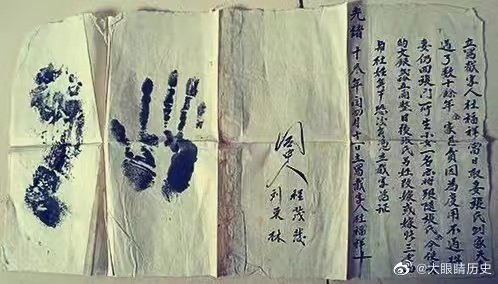
\includegraphics[height=0.36\textwidth,width=0.56\textwidth,viewport=0 0 375 240,clip]{Hand_and_foot-print.png}

\caption*{\hei\hspace{10pt}~

微博网页提供的清代光绪十八年~(公元1892年)~的休书}

\label{Collect_Liu_Wu}

\end{figure}\hspace{10pt}~

\includegraphics{.jpeg}

立写截字人杜福祥

当日娶妻张氏到家,夫妻过了数十余年。余家甚贫,因为度用不过,将妻仍回张门,所生小女一名,亦将跟随张氏。余今休妻的(得)文银贰拾伍两整,日后张氏另姓改嫁,或嫁张三、李四,与杜姓无干。恐说无凭,立截字为证。

\begin{flushright}

光绪十八年~闰四月十一日~立写截字人~~杜福祥 ~~(画 ``十字押'') ~~~\\

\large{同中人~程茂发、刘秉林} ~~~~~~~~~~~~~~~ \\

\huge{手模}、\huge{足印} ~~~~~~~~~~~

\end{flushright}
   %% 乌龙院
\newpage 
\phantomsection %实现目录的正确跳转
\section*{\large\hei 打鱼杀家~\protect\footnote{此戏是《庆顶珠》中的一部分,据有关资料载\upcite{WSZS2-78_2000},原《庆顶珠》全剧有``得宝''、``庆珠''、``比武''、``珠聘''、``打鱼''、``恶讨''、``屈责''、``献珠''、``杀家''、``投亲''、``劫牢''、``珠圆''等场次。一般习惯从``打鱼''演到``杀家'',故称《打鱼杀家》;~旧时戏单``鱼''、``渔''混用,亦作``打渔杀家''。据吴小如先生告,{\textrm 1949}年后因田汉建议,戏名统一为《打渔杀家》。}~{\small 之}~萧恩}
\addcontentsline{toc}{section}{\hei 打鱼杀家~{\small 之}~萧恩}

\hangafter=1                   %2. 设置从第1⾏之后开始悬挂缩进  %}
\setlength{\parindent}{0pt}{
{\vspace{3pt}{\centerline{{[}{\hei 第一场}{]}}}\vspace{5pt}}

{开船呐!}

{儿啊------}

\setlength{\hangindent}{56pt}{【{\akai 西皮摇板}】父女打鱼在河下,家贫哪怕人笑咱。拉住篷索父把网撒,}

\setlength{\hangindent}{56pt}{【{\akai 西皮散板}】年纪衰迈气力不佳。}

{唉,本当不做这河下生意,你我父女何以度日呀?}

{儿啊,不要啼哭,将船湾在柳荫之下,凉爽凉爽。}

{儿啊,将几尾鲜鱼烹煮好了,少时为父还要饮酒。}

{有人唤我。}

{是哪一位?}

{哦,原来是李贤弟。}

{敢莫要到舟中走走?}

{待我搭了扶手。}

{此位是------?}

{({\hwfs 惊介})这做什么?}

{老了,不中用了。}

{儿啊,出舱来见过二位叔父。}

{小女桂英。}

{一十六岁,痴长啊。}

{且慢,方才打得几尾鲜鱼,就在船头之上,你我弟兄畅快饮一回。}

{儿啊,看酒来。}

{啊,二位贤弟,愚兄有个酒令儿。}

愚兄做的是河下生意,忌的是``干''、``旱''二字。

不敢说罚,要敬酒三杯。

请------

呃,敬你三杯。

哦,待我看来。

诶!做什么的?

问的是哪一家呀?

你来看,就在前面,八字粉墙,合脊门楼,那就是丁$\cdots{}\cdots{}$

诶,哼,放肆!

量他也不敢呐。

请------

哦,又有人唤我。

二位贤弟再饮几杯。

哦,原来是丁郎儿,到此何事啊?

你来看,这几日天旱水浅,鱼不上网。改日有了银钱,送上府去。

哦,是是是。

放他去罢,

教他去罢。

(李俊、倪荣 啊,萧兄为何这等$\cdots{}\cdots{}$。)

他们的人多。

他们的势力大。

这就难讲话了。

本当不做河下生意,怎奈这囊中------唉,惭愧。

哪位贤弟送来?

当面谢过。

有了人家了。

花荣之子,名唤花逢春。

请------

二位贤弟慢走,愚兄不能远送了。

哦,来了。

儿问的是他?

儿啊------

\setlength{\hangindent}{56pt}{【{\akai 西皮摇板}】他本江湖二豪侠,倪荣、李俊就是他。蟒袍、玉带不愿挂,弟兄双双走天涯。}

\setlength{\hangindent}{56pt}{【{\akai 西皮散板}】猛抬头见红日坠落西斜。}

{儿啊,天色不早,我们回去了吧。}

{正是:~({\akai 念})父女打鱼在江下,}

{({\akai 念})堪堪不觉红日落,}

\vspace{3pt}{\centerline{{[}{\hei 第二场}{]}}}\vspace{5pt}

\setlength{\hangindent}{66pt}{【{\akai 西皮快三眼}】昨夜晚吃酒醉和衣而卧,稼场鸡惊醒了梦里南柯。二贤弟在河下相劝与我,他教我把打鱼的事啊一旦丢却。我本当不打鱼啊关门闲坐,怎奈我家贫穷无计奈何。清早起开柴扉乌鸦叫过,飞过来叫过去【{\footnotesize 转}{\akai 西皮二六}】却是为何。将身儿来至在草堂内坐,桂英儿取茶来为父解渴。}

{不教儿渔家打扮,怎么偏偏要渔家打扮?}

{呃------不听父言,就为不孝哇。}

{这便才是!}

{是哪个?}

{你们是哪里来的?}

{哦,原来是丁府上的教师爷。}

{哼!}

{做什么来了?}

{这几日天旱水浅,鱼不上网。改日有钱,送上府去,何必你来!}

{旁人来了无有,教师爷你来了么,}

{哼哼,越发的无有了!}

{朝廷王法,要它何用?}

{哼!}

{哼,尔要锁?}

{当真要锁?}

{果然要锁?}

{如此你就------锁!}

{不教锁。}

{哼!}

{话么,倒是两句好话呀,可惜呀可惜,}

{可惜你二大爷无有工夫啊。}

{尔要讲打?}

{诶呀!老汉幼年间,听说打架,如同小孩子穿新鞋、过新年的一般;如今呐------老了,打不动了啊!}

{尔当真要打?}

{果然要打?!}

{娃娃!待老汉将衣帽留在家中,打个样儿与你们见识见识。}

\setlength{\hangindent}{56pt}{【{\akai 西皮导板}】听一言不由我七窍冒火,}

\setlength{\hangindent}{56pt}{【{\akai 西皮摇板}】不由我年迈人咬碎牙车}\footnote{据樊百乐{\scriptsize 君}告知,刘曾复先生强调,``牙车''是``牙床''的意思。吴小如先生曾撰文指出,天津的王庾生先生此句唱作``这才是闭门坐平地生波''。}{。江湖上叫萧恩不才是我,}

\setlength{\hangindent}{56pt}{【{\akai 西皮摇板}】大战场、小战场见过许多。爷本是出山虎独自一个,}

\setlength{\hangindent}{56pt}{【{\akai 西皮摇板}】尔好比看家犬一群一窝。你本是奴下奴敢来欺我。}

{慢说是三``羊头'',就是尔这三``狗头'',二大爷何惧!}

{你是丁府上的教师爷?}

{你好本领呐!老汉要领教领教。}

{一定要领教。}

{这是大十八般武艺?}

{这小十八样兵器?}

{这拳脚是?}

{软硬功夫?}

{呃,这叫什么?}

{不好哇。}

{这叫什么?}

{呃,不好。}

{呃,越发的不好啊。}

{方才撞了老汉三``羊头'',如今我要打你三拳头,放你过去。}

{哪里有功夫。}

{着打!}

{着打!}

{打得好,只恐打出祸来了!}

{那贼回去,定不甘休。待为父赶至县衙,抢他一个原告!}

{不要儿管,取为父的衣帽过来。}

{好好看守门户,为父去去就来。}\footnote{陈超老师注:~刘曾复先生曾说明:~此处萧恩\textless{}\!{\bfseries\akai 扫头}\!\textgreater{}{\hwfs 下场},{\hwfs 不踢大带}:~{\hwfs 出门},{\hwfs 褶子倒手},{\hwfs 右手向上一指},{\hwfs 弹髯下}。这个\textless{}\!{\bfseries\akai 扫头}\!\textgreater{}扫的是一个``对儿'',``闭门家中坐,祸从天上来'',因此这一指表示``祸从天上来''。}

\vspace{3pt}{\centerline{{[}{\hei 第三场}{]}}}\vspace{5pt}

{\setlength{\hangindent}{52pt}{(萧桂英\hspace{20pt}【{\akai 西皮散板}】老爹爹清晨出前去出首,)}\footnote{刘曾复先生为樊百乐{\scriptsize 君}说《审刺客》一戏时,顺便说了``萧恩挨打''部分的内容。} }

{(众\hspace{40pt}({\akai 内})一十!)}

{(萧桂英\hspace{20pt}【{\akai 西皮散板}】倒叫我桂英儿挂在心头。)}

{(众\hspace{40pt}({\akai 内})二十!)}

{(萧桂英\hspace{20pt}【{\akai 西皮散板}】将身儿来至在草堂门口,)}

{(众\hspace{40pt}({\akai 内})三十!)}

{(萧桂英\hspace{20pt}【{\akai 西皮散板}】只等得爹爹回细问根由。)}

{(众\hspace{40pt}({\akai 内})四十打完!)}

{(吕子秋\hspace{20pt}({\akai 内})赶下堂去!)}

{好贼!}

\setlength{\hangindent}{56pt}{【{\akai 西皮散板}】恼恨那吕子秋为官不正,仗势力欺压我受苦的良民呐。上堂来他那里一言不问,责打我四十板呐赶出了头门。}

\setlength{\hangindent}{56pt}{【{\akai 西皮散板}】我这里咬牙关忙往家奔,叫一声桂英儿你快来开门{\footnotesize 呐}。}

{为父上得堂去,那贼一言不问,将为父重责。}

{这还不算受屈。他教为父连夜过江与那老贼赔礼,那才算受屈呢。}

{哎呀------我恨不得飞过江去,我就杀$\cdots{}\cdots{}$}

{我要杀贼的满门,方消我心头之恨!}

{小小年纪,懂得什么?!不用多管,取为父衣帽、戒刀过来。}

{不用儿管,快些取来。}

{为父去也。}

{何事?}

{小小年纪,去之无益。}

{有此胆量?}

{快将儿的衣服、兵刃收拾好了。}

{壮胆量也是好的。}

{走哇$\cdots{}\cdots{}$}

{做什么?}

{这门么,关也罢,不关也罢呀。}

{又做什么?}

{唉!门都不要了,还要什么家具呀?}

{唉,不明白的冤家呀,呃$\cdots{}\cdots{}$({\hwfs 哭介})}

{不要啼哭,随为父的走哇。}

{儿啊,此番前去,教儿骂,儿就骂,教儿杀,儿就杀,不要害怕。}

{走哇。}

{儿啊,夜晚行船,比不得白日,儿要掌稳了舵!}

\setlength{\hangindent}{56pt}{【{\akai 西皮快板}】这件事不由我心头冒火,今夜晚过江去将他杀却。恨不得插双翅江河越过,}

\setlength{\hangindent}{56pt}{【{\akai 西皮散板}】我的儿因何故放了篷索。}

{杀人还有什么假的不成?}

{呀呸!为父在家中不教儿前来,儿是偏偏地要来。这船行半江之中,儿又要回去------也罢!待为父拨转船头,送儿回去。}

{\textless{}\!{\bfseries\akai 哭头}\!\textgreater{}啊,桂英,我的儿呀!}

{少时还在此处上船,儿记下了?}

{儿啊,庆顶珠\footnote{吴小如先生告,萧恩对萧桂英提及``庆顶珠''时,念白作``聘礼珠子'',``庆顶珠''留作戏名。}可在身旁?}

{此番前去,倘有不测,儿自带庆顶珠逃往花家去吧。}

{我么------儿就不用管了哇。}

{不要啼哭,随我走哇。}

{来此已是。}

{且慢。}

{收拾好了。}

{有人么?走出一个来呀。}

{过府赔罪来了。}

{哼!}

{请了。}

{我来问你:~这鱼税银子,可有圣上旨意?}

{户部公文?}

{凭着何来?}

{敢是那吕子秋?!}

{哼!}

\setlength{\hangindent}{56pt}{【{\akai 西皮摇板}】这税银我不纳是我的本分,你不该差人役打上我门。}

{儿啊,骂呀!}

{且慢,我父女有好心献上。}

{打鱼之时,得来一宗宝贝,名唤庆顶珠。}

{这$\cdots{}\cdots{}$耳目甚多。}

{看刀!}

{儿啊,随为父的杀呀!}

}
   %% 打鱼杀家
\newpage
\phantomsection %实现目录的正确跳转
\section*{\large\hei {硃砂痣~{\small 之}~韩廷凤}~({\hwl 谭派})}
\addcontentsline{toc}{section}{\hei 硃砂痣~{\small 之}~韩廷凤}

\hangafter=1                   %2. 设置从第1⾏之后开始悬挂缩进  %}
\setlength{\parindent}{0pt}{

{\vspace{3pt}{\centerline{{[}{\hei 第一场}{]}}}\vspace{5pt}}

{唉!}

\setlength{\hangindent}{56pt}{【{\akai 二黄摇板}】为续弦前后厅灯光明亮,梦不想今夜晚再做新郎。}

{抬上堂来({\akai 或}:~}搭上堂来)\footnote{以下括号中的念白据吴焕老师整理的剧本(经刘曾复先生审订)添加。}{。}

{每人赏银二分({\akai 或}:~}每人赏钱四个){。}

{带他们下面用饭。}

{待我观看一回。}

\setlength{\hangindent}{56pt}{【{\akai 二黄慢板}】我这里借灯光用目观望,我看她({\akai 或}:~只见她)与前妻一样风光。}

\setlength{\hangindent}{56pt}{【{\akai 二黄慢板}】为什么({\akai 或}:~因何故)皱眉间泪带面上({\akai 或}:~泪带脸上),莫不是嫌年迈难配鸾凰。}

\setlength{\hangindent}{56pt}{【{\akai 二黄慢板}】要穿衣锦绣衫任你选样,}

\setlength{\hangindent}{56pt}{【{\akai 二黄慢板}】要用饭现有那谷米陈仓。}

\setlength{\hangindent}{56pt}{【{\akai 二黄慢板}】这不是那不是难以猜想,尊娘行({\akai 或}:~问娘行)因何事珠泪汪汪,为的是哪桩,你何妨({\akai 或}:~又何妨)细说端详?}

\setlength{\hangindent}{56pt}{【{\akai 二黄摇板}】听她言这婚姻({\akai 或}:~好一似)冰结霜降,一时里惹动我烦恼愁肠。看起来断不可此事勾当,自情愿伴孤灯独守空房。}

{韩福过来。}

{命你同媒婆送这位大娘子回去,对他丈夫言讲({\akai 或}:~与他丈夫言讲):~前番(那)一百两银子不要,再送他一百两银子,教他好好将养疾病,将大娘子送回,成全他夫妻恩义。就此去罢。}

{啊大娘子,还有这婚书呢。}

{唉,就在灯前焚化了罢。}

\setlength{\hangindent}{56pt}{【{\akai 二黄摇板}】已言道\footnote{此处《传统京剧汇编》第八集~伍月华~藏本作``曾言道'';~李楠{\scriptsize 君}建议作``既言道''似亦可。}她丈夫病卧床上,没奈何卖妻子暂度时光。将自己比旁人俱是({\akai 或}:~皆是)一样,我岂肯拆散他恩爱鸳鸯。({\akai 或}:~善与恶自有那天理昭彰。)}

{\vspace{3pt}{\centerline{{[}{\hei 第二场}{]}}}\vspace{5pt}}

\setlength{\hangindent}{69pt}{【{\akai 二黄摇板}\footnote{据吴焕老师整理的剧本注:~汪派在``想当年''前面还有两句,词句是``劝世人一个个须要学好,皆因是自有那天理昭彰。''}{】想当年为太守何等荣耀,遇兵荒妻和子无有下梢。多亏了陈太尉将我来保,才能得归田园自在逍遥。}

\setlength{\hangindent}{56pt}{【{\akai 二黄摇板}】忙迫中{\footnotesize 呃}挽定了把礼还到,一时里好教我难解根苗。}

{呜,你不是昨晚送回去的大娘子么?}

{既然将你送回,你又来则甚呐?}

{哦,(原来是)吴相公来了。}

{哎呀,请坐请坐。}

{呃,还有话讲啊。}

{(有话叙谈,}哪有不坐之理,请坐请坐。{)}

{啊大娘子,你也坐下。}

{啊吴相公,昨日听得大娘子说到家中一番苦楚,甚是凄惨。相公有恙在身,改日再来叙谈,为何带病前来?({\akai 或}:~大相公,昨日听得大娘子说到家中一番苦楚。相公你有病在床,病体好了,再来不迟。)}

{哦,你见了银子,出了一身的通汗,这病就好了么?}

{哎呀呀,吴相公啊,看将起来,这银子啊,是好物件!}

\setlength{\hangindent}{76pt}{【{\akai 二黄碰板垛板}】我救你的急,救你的难,救你的贫困;~全尔的节,全尔的义,全尔的婚{\footnotesize 呐}姻。纵有妻不生子前生造定,我岂肯拆婚姻\footnote{此处刘曾复先生说戏录音近似``错婚姻'',吴小如先生从夏山楼主学的是``拆婚姻'',此处从吴小如先生。李楠{\scriptsize 君}认为,此处系刘曾复先生将``拆''字按上口字处理。}落下了骂名。}

{啊,啊,呵呵呵哈哈哈$\cdots{}\cdots{}$({\hwfs 笑介})}

{请坐请坐。}

{哎呀呀吴相公啊,我当日也是恩爱夫妻,只因兵荒马乱,中途失散,却无子嗣。若有一子传宗接代,我也就不续弦再娶的了哇。}

{这$\cdots{}\cdots{}$子孙前世所修,再续么,也就不必了。({\akai 或}:~}子孙之事,前生所修。再娶么,唉,也就不必了。{)}

{言得极是,只是本处孩儿多有不便呐。}

{本当如此,奈无机会。}

{这只好凭天机、遇时宜了。}

{吴相公慢些走啊!}

\setlength{\hangindent}{56pt}{【{\akai 二黄摇板}】他夫妻进门来双双拜倒({\akai 或}:~双双跪倒),口声声叫恩人泪似{\footnotesize 呃}雨抛。非是我用银钱假意行好哇,韩廷凤全仁义一片心苗。}

{\vspace{3pt}{\centerline{{[}{\hei 第三场}{]}}}\vspace{5pt}}

\setlength{\hangindent}{46pt}{【{\akai 四平调}】叹光阴去不归无限烦闷,不觉已老两鬓如银。读古书难解我心头烦闷,饮香醪怎畅我衷肠凄清。}

{哦,你是吴相公,呃,请坐请坐。}

{你往成都收取账目,呃,必定是发了财了哇。({\akai 或}:~}闻你往成都,收取账目,一定发财的了。{)}

{请便。}

{哦,这是何人?}

{哦,罢了(罢了),一旁坐下。}

{呃,不妨不妨,只管地坐下。}

{呵呵呵哈哈哈$\cdots{}\cdots{}$({\hwfs 笑介})}

{啊吴相公,你看这小小的孩童,呃,也(很)知大体呀。}

{是啊,小孩子原要(他)爹娘教导哇。}

{啊吴相公,你买他前来,还是为子啊,还是为仆呢?}

{哦,这等说来({\akai 或}:~}如此说来){,是送与我的?}

{哎呀呀吴相公啊,你真是({\akai 或}:~}你真乃){信实人也。}

\setlength{\hangindent}{56pt}{【{\akai 四平调}】吴官人你真真言而有信,你与我谋后代不惜辛勤。感谢你这好意情深义尽,\textless{}\!{\bfseries\akai 行弦}\!\textgreater{}}

{吴大哥,你请来上坐。({\akai 或}:~这边坐,这边坐。)}

{请坐,请坐。}

\setlength{\hangindent}{56pt}{【{\akai 四平调}】退一日自当另有条陈。}

{呵呵哈哈哈$\cdots{}\cdots{}$({\hwfs 笑介})}

{哎呀吴官人呐,我如今有了儿子就不愁了。}

{是啊,吴官人离家日久,我也不便相留({\akai 或}:~不便强留),改日我父子要登门叩谢。}

{儿啊,送过你吴大爷。}

{(啊,吴官人何事?)}

{请来吃酒,请来吃酒。}

{啊$\cdots{}\cdots{}$呃,吴官人,请转请转。}

{改日我父子,呃,要登门再谢。}

{呃一定要去,一定要去。}

{啊$\cdots{}\cdots{}$呃,无有了,请便请便。({\akai 或}:~吴官人,请呐请呐。)}

{哦------哈哈哈$\cdots{}\cdots{}$({\hwfs 笑介})}

{儿啊,随为父的进来。}

{一旁坐下,待我细看一回({\akai 或}:~待我}细观一回{)。}

\setlength{\hangindent}{56pt}{【{\akai 二黄原板}】我的儿须从容端然坐定,看形象并非是平等\footnote{这里平等是``地位普通、平凡''之意。包玥{\scriptsize 君}认为作``贫等'',似亦通。此处从吴焕老师整理的剧本。}之人。细观他各部位五官端正,这两鬓齐开朗目秀眉清。儿在家可读过圣贤书本,一一地对为父细说分明。}

\setlength{\hangindent}{56pt}{【{\akai 二黄原板}】他说话有分寸智慧聪明,倒像个宦门后不差毫分。可记得是何年月日生辰,说出来将八字细与儿评。}

\setlength{\hangindent}{56pt}{【{\akai 二黄原板}】这小娃言语中隐藏暗景,再问他亲父母便知真情。儿父母年多少在不在,因何故图银钱卖与他人。}

{儿今年多大年纪了({\akai 或}:~}儿今年几岁了{) ?}

{儿父?}

{死了五载。}

{儿母?}

{七旬有余。}

{(惊{\hwfs 介})儿有一十三岁({\akai 或}:~}儿才一十三岁{)。}

{(惊{\hwfs 介})嗯$\cdots{}\cdots{}$}

\setlength{\hangindent}{56pt}{【{\akai 二黄原板}】这其间又盘出}\footnote{吴焕老师整理的剧本记作``又攀出''。}{奇情种种,哪有个花甲年又产娇生。}

{儿啊------}

\setlength{\hangindent}{56pt}{【{\akai 二黄原板}】必然是那老娘将儿蒙混,这内中另有个生儿的娘亲。}

{哦,儿是捡来的么?}

\setlength{\hangindent}{56pt}{【{\akai 二黄原板}】细盘问这来由日月推论,仔细想当年事越加是真:~宣和年四月里成都调任,行至在青州府路遇贼兵。亲生儿在娘怀无有踪影,实可怜贤德妻命赴幽冥。}

\setlength{\hangindent}{56pt}{【{\akai 二黄散板}】这形象好一似韩门真种\footnote{李楠{\scriptsize 君}认为此处``真种''作``真胤''更符合辙口。},举动间与老夫骨肉有情。我这里取菱花照照相品呐,}

\setlength{\hangindent}{56pt}{【{\akai 二黄散板}】半像我半像妻不差毫分。}

\setlength{\hangindent}{56pt}{【{\akai 二黄散板}】亲生子再相逢三生有幸,这才是天地意弄假成真。}

{不对了,不对了!}

{(韩玉印\hspace{20pt}怎么不对呢?)}

{我那亲生的孩儿,落生下来,左足心上有硃砂红痣。你无有,不是我的亲生儿子啊。}

{怎么,儿也有?}

{为父的不信呐,待我看来。}

{(唉,儿啊------)}

\setlength{\hangindent}{56pt}{【{\akai 二黄散板}】你是我亲生的儿呀名唤玉印,遇兵荒遭失散十有二春。盼娇儿盼得我身染重病,盼娇儿盼得我昼夜不宁。盼娇儿啊不做官告归故呃井,喂呀我的儿呀,梦不想天保佑枯木哇逢春。}

{你母命丧东平,也曾命人搬尸去了$\cdots{}\cdots{}$哇,呃$\cdots{}\cdots{}$({\hwfs 哭介})}

{言得极是,派人接她前来就是。}

{正是:~({\akai 念})北转南来西复东,今朝骨肉又重逢。父子再把菱花照,}

{(儿啊------)}

{({\akai 念})只怕相逢在梦中。}

{哦,不是做梦?}

{玉印,我儿,啊------啊------哈哈哈$\cdots{}\cdots{}$({\hwfs 笑介})}

{随我来。}
   %% 硃砂痣
\newpage
\phantomsection %实现目录的正确跳转
\section*{\large\hei {雄州关}}
\addcontentsline{toc}{section}{\hei 雄州关}

\hangafter=1                   %2. 设置从第1⾏之后开始悬挂缩进  %}}
\setlength{\parindent}{0pt}{

\vspace{3pt}{\centerline{{[}{\hei 第一场}{]}}}\vspace{5pt}

\setlength{\hangindent}{52pt}{{呼延狄\hspace{20pt}({\akai 念})百万熊罴犯中原,}}

\setlength{\hangindent}{52pt}{{雷洪切\hspace{20pt}({\akai 念})搅乱宋室不安然!}}

\setlength{\hangindent}{52pt}{{达林呈\hspace{20pt}({\akai 念})渴饮马上刀头血,}}

\setlength{\hangindent}{52pt}{{季乐芬\hspace{20pt}({\akai 念})嘿!饥饿人头当饭餐!}}

\setlength{\hangindent}{52pt}{{众\hspace{40pt}俺------}}

\setlength{\hangindent}{52pt}{{呼延狄\hspace{20pt}金邦大将军呼延狄是也!}}

\setlength{\hangindent}{52pt}{{雷洪切\hspace{20pt}金邦副将军雷洪切是也!}}

\setlength{\hangindent}{52pt}{{达林呈\hspace{20pt}金邦左先锋达林呈是也!}}

\setlength{\hangindent}{52pt}{{季乐芬\hspace{20pt}金邦右先锋季乐芬是也!}}

\setlength{\hangindent}{52pt}{{萨里哈\hspace{20pt}前营骁骑大将军萨里哈是也!}}

\setlength{\hangindent}{52pt}{{耶律浑\hspace{20pt}后营骁骑大将军耶律浑是也!}}

\setlength{\hangindent}{52pt}{{提尔雄\hspace{20pt}左营压队大将军提尔雄是也!}}

\setlength{\hangindent}{52pt}{{虎骨达\hspace{20pt}右营护卫大将军虎骨达是也!}}

\setlength{\hangindent}{52pt}{{呼延狄\hspace{20pt}列位将军请了------}}

\setlength{\hangindent}{52pt}{{众\hspace{40pt}请了!}}

\setlength{\hangindent}{52pt}{{呼延狄\hspace{20pt}你我奉了狼主之命,随定四太子,领兵夺取宋室天下,兵到即克。也是宋王气数当尽了。}}

\setlength{\hangindent}{52pt}{{众\hspace{40pt}着啊!}}

\setlength{\hangindent}{52pt}{{呼延狄\hspace{20pt}这些蛮子怎能苦争恶战,这也是我家狼主洪福齐天也!}}

\setlength{\hangindent}{52pt}{{众\hspace{40pt}听觱篥}\footnote{段公平{\scriptsize 君}注:~觱篥,又作``筚篥'',竹管乐器,源于西域,类似``胡笳''。即俗称``牛角觱篥''者,番邦号角。}{一声响,太子升帐,你我两厢伺候。请------}}

\setlength{\hangindent}{52pt}{{金兀朮\hspace{20pt}\textless{}\!{\bfseries\akai 点绛唇}\!\textgreater{}军营号响}\footnote{段公平{\scriptsize 君}建议作``各路豪强''。}{,威武雄壮;~中军帐,排列刀枪,杀气{\footnotesize 呃}------}}

\setlength{\hangindent}{52pt}{{众\hspace{40pt}参见殿下!}}

\setlength{\hangindent}{52pt}{{金兀朮\hspace{20pt}站立两厢!}}

\setlength{\hangindent}{52pt}{{金兀朮\hspace{20pt}({\akai 念})杀气腾腾满乾坤,哀声处处震天庭。宋王失政宠奸佞,锦绣江山一旦倾。}}

\setlength{\hangindent}{52pt}{{金兀朮\hspace{20pt}孤,北番大金邦女真国老王殿下四太子、昌平王、御营总兵完颜兀朮。今有宋主无道,宠信奸臣。内奸童贯封为广阳王}\footnote{此处从《传统剧目汇编》,童贯封``广阳王''。}{之职。是他前者有密书到孤父王驾下,约定我国兴兵夺取他家社稷。有他以为内应,这宋室天下岂不是唾手而得。自兴兵以来,战无不胜,攻无不取。前日又破了潞安州,守将陆登自刎身亡,甚是悲惨。前面乃是雄州关,守将韩世忠。此人乃是忠勇之士,孤家不忍逼迫于他。意欲招他归顺,助孤一臂之力,何愁大事不成。}}

\setlength{\hangindent}{52pt}{{金兀朮\hspace{20pt}众番儿!}}

\setlength{\hangindent}{52pt}{{众\hspace{40pt}有!}}

\setlength{\hangindent}{52pt}{{金兀朮\hspace{20pt}此番兴兵行至雄州关,不可杀掠黎民,违令者斩!}}

\setlength{\hangindent}{52pt}{{众\hspace{40pt}啊!}}

\setlength{\hangindent}{52pt}{{金兀朮\hspace{20pt}由此发动人马!}}

\vspace{3pt}{\centerline{{[}{\hei 第二场}{]}}}\vspace{5pt}

\setlength{\hangindent}{52pt}{{探子\hspace{30pt}马来。}}

\setlength{\hangindent}{52pt}{{探子\hspace{30pt}({\akai 念})短甲随身衲袄齐,肩上横担令字旗。年年岁岁领皇赏。一马冲至军队里。}}

\setlength{\hangindent}{52pt}{{探子\hspace{30pt}俺,韩元帅麾下能行探子是也。奉了元帅将令,着俺四路哨探。今有圣上差孙浩督兵前来剿灭金邦,已至三山口。不免飞骑报韩元帅知道!就此马上加鞭。}}

\vspace{3pt}{\centerline{{[}{\hei 第三场}{]}}}\vspace{5pt}

\setlength{\hangindent}{52pt}{{韩世忠\hspace{20pt}【{\akai 西皮三眼}】为金兵急得我心神不定,盼救}兵望眼穿昼夜不宁。陆元帅尽了忠自刎丧命,只一子失陷在万马军营。好教人止不住啊【{\footnotesize 转}{\akai 西皮二六}】腮边泪滚,可叹他夫妻们饮恨幽冥。行公文\footnote{夏行涛{\scriptsize 君}建议作``赍公文''。}求圣上遣将助阵,因何故十数日渺无回音。在二堂思无计心呃中忧闷,我父子只恐怕难退雄兵。}

\setlength{\hangindent}{52pt}{中军\hspace{30pt}({\akai 念})探马如飞急,叩禀元帅知。}

\setlength{\hangindent}{52pt}{中军\hspace{30pt}启元帅:~探马求见。}

\setlength{\hangindent}{52pt}{韩世忠\hspace{20pt}吩咐开门!}

\setlength{\hangindent}{52pt}{中军\hspace{30pt}开门!}

\setlength{\hangindent}{52pt}{众\hspace{40pt}啊!}

\setlength{\hangindent}{52pt}{韩世忠\hspace{20pt}{({\akai 念})}探马报音信,升帐问分明。}

\setlength{\hangindent}{52pt}{韩世忠\hspace{20pt}传探马。}

\setlength{\hangindent}{52pt}{中军\hspace{30pt}元帅有令:~探马进见。}

\setlength{\hangindent}{52pt}{探马\hspace{30pt}报------告进。}

\setlength{\hangindent}{52pt}{探马\hspace{30pt}帅爷在上,探马叩头。}

\setlength{\hangindent}{52pt}{韩世忠\hspace{20pt}打听哪路军情,起来快些讲。}

\setlength{\hangindent}{52pt}{探马\hspace{30pt}啊,帅爷听禀:~}

\setlength{\hangindent}{52pt}{探马\hspace{30pt}({\akai 念})一马哨探似流星,朝中差来孙总兵。十万人马到疆界,禀报元帅得知情。}

\setlength{\hangindent}{52pt}{韩世忠\hspace{20pt}朝中无有什么姓孙的呀!}

\setlength{\hangindent}{52pt}{探马\hspace{30pt}在元帅帐下当过副将的。}

\setlength{\hangindent}{52pt}{韩世忠\hspace{20pt}哦------敢是孙浩?!}

\setlength{\hangindent}{52pt}{探马\hspace{30pt}正是。}

\setlength{\hangindent}{52pt}{韩世忠\hspace{20pt}赏尔金牌一面,再去打探。}

\setlength{\hangindent}{52pt}{探马\hspace{30pt}得令!}

\setlength{\hangindent}{52pt}{韩世忠\hspace{20pt}且住!想那孙浩,在某帐下曾为副将。只因犯我将令,将他捆打,是他逃至京中,投在{广阳}府内,做了随侍。今番奉旨督兵前来,焉有不接之理。}

\setlength{\hangindent}{52pt}{韩世忠\hspace{20pt}中军!}

\setlength{\hangindent}{52pt}{中军\hspace{30pt}有!}

\setlength{\hangindent}{52pt}{韩世忠\hspace{20pt}传众将进帐。}

\setlength{\hangindent}{52pt}{中军\hspace{30pt}众将进帐呃!}

\setlength{\hangindent}{52pt}{四将\hspace{30pt}({\akai 内})来也!}

\setlength{\hangindent}{52pt}{四将\hspace{30pt}({\akai 念})元帅传军令,将士共趋迎\footnote{夏行涛{\scriptsize 君}建议作``躬躯迎''。}。}

\setlength{\hangindent}{52pt}{四将\hspace{30pt}参见元帅。}

\setlength{\hangindent}{52pt}{韩世忠\hspace{20pt}众位将军少礼!}

\setlength{\hangindent}{52pt}{四将\hspace{30pt}啊!}

\setlength{\hangindent}{52pt}{四将\hspace{30pt}传末将等进帐,有何军情议论?}

\setlength{\hangindent}{52pt}{韩世忠\hspace{20pt}圣上命孙浩督兵前来,征剿金人,已到三山口。命你等前去迎接。}

\setlength{\hangindent}{52pt}{四将\hspace{30pt}啊元帅,那孙浩若问:~你家元帅为何不来。我等怎样回答?}

\setlength{\hangindent}{52pt}{韩世忠\hspace{20pt}你等就说:~我家元帅因金兵犯境,城内空虚,不敢擅离汛地,故命我等前来迎接。}

\setlength{\hangindent}{52pt}{四将\hspace{30pt}那孙浩缘何授得此职?}

\setlength{\hangindent}{52pt}{韩世忠\hspace{20pt}唉!你等不知他的来历,听我令下:~}

\setlength{\hangindent}{52pt}{{韩世忠\hspace{20pt}【{\akai 西皮}原板}】韩世忠坐宝帐传言发令,叫一声众将官细听详情:~那孙浩平日间行为不正,犯军令责罚他不能徇情呃。逃到了京师地{广阳}府进,童太尉听谗言懵懂圣君。迎接他务须要言语谨慎,}

\setlength{\hangindent}{52pt}{{韩世忠\hspace{20pt}【{\akai 西皮摇板}】防贼子寻仇起暗箭伤人。}

\setlength{\hangindent}{52pt}{{四将\hspace{30pt}得令!}}

\setlength{\hangindent}{52pt}{{四将\hspace{30pt}【{\akai 西皮摇板}】韩元帅忠义士谁人不敬,何惧那孙浩贼势利小人。}}

\setlength{\hangindent}{52pt}{{韩世忠\hspace{20pt}【{\akai 西皮摇板}】大宋朝八代君徽宗失政,贪酒色戮忠良信宠谗臣。恨蔡京与童贯伤害民命,惹得那四路里齐动刀兵。金兀朮领人马抢夺州郡,逼元戎劳将士苦及黎民。众将官退宝帐各归管汛,}}

\setlength{\hangindent}{52pt}{{韩世忠\hspace{20pt}【{\akai 西皮摇板}】且等候四将回再定计行。}}

\vspace{3pt}{\centerline{{[}{\hei 第四场}{]}}}\vspace{5pt}

\setlength{\hangindent}{52pt}{{孙浩\hspace{30pt}\textless{}\!{\bfseries\akai 点绛唇}\!\textgreater{}奉旨领雄兵,蟒罗袍,不愧先人;~定斩世忠消吾恨,还报他痛打军刑。}}

\setlength{\hangindent}{52pt}{孙浩\hspace{30pt}({\akai 念}){胸怀巧诈极聪明,不近贵人怎升腾?只道一生空劳力,运至时来命通亨。}}

\setlength{\hangindent}{52pt}{{孙浩\hspace{30pt}某,孙浩,塞北人也。昔在韩世忠麾下以为步军,只因不守军规,专意花酒情浓。抢得一有夫之妇作乐,不想韩世忠便要将俺斩首。是俺推在步兵列名身上,彼时将那步兵斩首号令。又道俺带领无方,将俺捆打,削去头领,赶出不用。俺又羞又恼,一怒奔至京中。恰遇童太尉朝罢而归,是俺闯了他的禁道,将我拿到府中拷问。俺将韩世忠打革之事从头诉说一遍,不想童太尉与韩世忠是旧有仇恨,听了此言,便把俺留在府呃中。因俺善于奉承,是他心中欢喜,想要重用于俺。如今金兀朮兴兵犯界,破了无数城池。眼看要到雄州,那韩世忠本章进京,求兵添将。童太尉奏上一本,命俺提兵前来,剿灭番贼。若是得胜,道韩世忠贪生怕死;~若是损兵,便道韩世忠按兵不动。慢说是一个韩世忠,就是百个,也教他有死无生。看前面已是三山口,众将,催动人马!}}

\setlength{\hangindent}{52pt}{{孙浩\hspace{30pt}【{\akai 西皮导板}】见旌旗空中飘人声喧震,}}

\setlength{\hangindent}{52pt}{{孙浩\hspace{30pt}【{\akai 西皮原板}】抖起}了万丈尘沸沸腾腾。曾记得到京都那般光景,岂料我今日里督领雄兵。韩世忠好比那儿童之分,怎知晓暗中刀要你残生。咱料他如南柯梦魂未醒,}

\setlength{\hangindent}{52pt}{{孙浩\hspace{30pt}【{\akai 西皮摇板}】绑云阳一命倾才晓前情。}

\setlength{\hangindent}{52pt}{{孙浩\hspace{30pt}前道}\footnote{段公平{\scriptsize 君}建议作``前导''。}{为何不行?}}

\setlength{\hangindent}{52pt}{{四将\hspace{30pt}雄州关总戎麾下四营将校迎接总爷。}}

\setlength{\hangindent}{52pt}{{众\hspace{40pt}雄州关总戎麾下四营将校迎接总爷。}}

\setlength{\hangindent}{52pt}{{孙浩\hspace{30pt}传。}}

\setlength{\hangindent}{52pt}{{众\hspace{40pt}传。}}

\setlength{\hangindent}{52pt}{{四将\hspace{30pt}雄州关四营将校迎接总爷}}

\setlength{\hangindent}{52pt}{{孙浩\hspace{30pt}你家主帅有多大的官儿,怎么不来迎接本镇。}}

\setlength{\hangindent}{52pt}{{四将\hspace{30pt}启禀总爷:~主帅为金兵临界,关内空虚,不敢擅离汛地,故而命末将等前来迎接总爷。}}

\setlength{\hangindent}{52pt}{{孙浩\hspace{30pt}哼------你住了!本镇钦奉圣命,广阳王钧旨,领兵剿贼,你们主帅也不看在眼内,本当将尔等捆打------}}

\setlength{\hangindent}{52pt}{{四将\hspace{30pt}总爷开恩。}}

\setlength{\hangindent}{52pt}{{孙浩\hspace{30pt}也罢!待本镇破了金兵回来,再与你主帅辩理。}}

\setlength{\hangindent}{52pt}{{孙浩\hspace{30pt}来呀,乱棍逐出!}}

\setlength{\hangindent}{52pt}{{孙浩\hspace{30pt}催------军!}}

\setlength{\hangindent}{52pt}{{孙浩\hspace{30pt}【{\akai 西皮摇板}】定教他主帅们无处逃奔,少不得斩尔等碎尸粉身。叫众将越过了飞龙奇岭,扫灭了番邦贼奏达捷音。}}

\vspace{3pt}{\centerline{{[}{\hei 第五场}{]}}}\vspace{5pt}

\setlength{\hangindent}{52pt}{{韩世忠\hspace{20pt}【{\akai 西皮摇板}】命四将接孙浩渺无音信,倒教我背地里暗自思忖呐。必然他要报那从先的仇恨,可惜我空费了一片精神。}}

\setlength{\hangindent}{52pt}{{四将\hspace{30pt}【{\akai 西皮摇板}】贼孙浩忒无礼令人可恨,全不念数年间共事同营。}}

\setlength{\hangindent}{52pt}{{四将\hspace{30pt}参见元帅!}}

\setlength{\hangindent}{52pt}{{韩世忠\hspace{20pt}你们回来了。}}

\setlength{\hangindent}{52pt}{{四将\hspace{30pt}回来了。}}

\setlength{\hangindent}{52pt}{{韩世忠\hspace{20pt}迎接孙浩他可曾讲些什么?}}

\setlength{\hangindent}{52pt}{{四将\hspace{30pt}末将等奉令迎接孙浩,那厮言道:~你家主帅为何不来?}}

\setlength{\hangindent}{52pt}{{韩世忠\hspace{20pt}你等怎生回答?}}

\setlength{\hangindent}{52pt}{{四将\hspace{30pt}末将言道:~金兵临界,城内空虚,不敢擅离汛地,故命我等前来迎接}}

\setlength{\hangindent}{52pt}{{韩世忠\hspace{20pt}那厮如何言道?}}

\setlength{\hangindent}{52pt}{{四将\hspace{30pt}那厮言道:~本镇钦奉圣命,广阳王钧旨,领兵剿贼,你主帅有多大的官儿,不来迎接本镇。本当将尔捆绑------待等破了金兵回来,再与你主帅辩理。说罢此言,呃,将我等乱棍,呵,逐出来了。}}

\setlength{\hangindent}{52pt}{{韩世忠\hspace{20pt}小人得志,以致如此。}}

\setlength{\hangindent}{52pt}{{探子\hspace{30pt}报!启禀元帅:~孙浩越过飞龙岭,迎战金兵去了。}}

\setlength{\hangindent}{52pt}{{韩世忠\hspace{20pt}再探!}}

\setlength{\hangindent}{52pt}{{韩世忠\hspace{20pt}且住!我想孙浩越过飞龙岭与金兵迎战,倘有差池本帅难逃罪责。}}

\setlength{\hangindent}{52pt}{{韩世忠\hspace{20pt}来,传彦直进帐。}}

\setlength{\hangindent}{52pt}{{中军\hspace{30pt}有请少将军。}}

\setlength{\hangindent}{52pt}{{韩彦直\hspace{20pt}来也!}}

\setlength{\hangindent}{52pt}{{韩彦直\hspace{20pt}({\akai 念})战国英雄数伍员,一忿扫平楚国兵。}}

\setlength{\hangindent}{52pt}{{韩彦直\hspace{20pt}参见父帅。}}

\setlength{\hangindent}{52pt}{{韩世忠\hspace{20pt}罢了!坐下。}}

\setlength{\hangindent}{52pt}{{韩彦直\hspace{20pt}谢座。唤孩儿进帐,有何吩咐?}}

\setlength{\hangindent}{52pt}{{韩世忠\hspace{20pt}圣上命孙浩督兵前来,征剿金人,那贼从飞龙岭迎敌去了。命你带领人马,暗地保护,需要小心在意,听为父令下:~}}

\setlength{\hangindent}{52pt}{{韩世忠\hspace{20pt}【{\akai 西皮摇板}】广阳王点孙浩身当重任,命四将迎接他赶回州城。我的儿领人马暗地接应,钦命官须保护谨慎小心。}}

\setlength{\hangindent}{52pt}{{韩彦直\hspace{20pt}得令!}}

\setlength{\hangindent}{52pt}{{韩彦直\hspace{20pt}【{\akai 西皮摇板}】在帐中领将令怎敢迟顿,暗地里保孙浩谨慎殷勤。}\footnote{刘曾复先生介绍,此处唱下是程继先的演法,金仲仁的演法是念下。}}

\setlength{\hangindent}{52pt}{{韩世忠\hspace{20pt}众将官,随本帅披挂,催动人马,起兵前往!}}

\vspace{3pt}{\centerline{{[}{\hei 第六场}{]}}}\vspace{5pt}

\setlength{\hangindent}{52pt}{{金兀朮\hspace{20pt}马前来的将官,可是韩元帅?}}

\setlength{\hangindent}{52pt}{{孙浩\hspace{30pt}逆贼,俺乃童太尉府中的心腹之人,剿贼大将军孙浩是也!}}

\setlength{\hangindent}{52pt}{{金兀朮\hspace{20pt}奸贼一党,休要放走之呃!}}

\vspace{3pt}{\centerline{{[}{\hei 第七场}{]}}}\vspace{5pt}

\setlength{\hangindent}{52pt}{{韩彦直\hspace{20pt}({\akai 念})头戴束发紫金冠,金锁铠甲扣连环。胸怀重瞳英雄胆,宝剑出鞘血未干。}}

\setlength{\hangindent}{52pt}{{韩彦直\hspace{20pt}俺,韩彦直。奉了父帅之命,暗地保护孙浩。}}

\setlength{\hangindent}{52pt}{{韩彦直\hspace{20pt}众将官!}}

\setlength{\hangindent}{52pt}{{众\hspace{40pt}有!}}

\setlength{\hangindent}{52pt}{{韩彦直\hspace{20pt}杀上前去!}}

\vspace{3pt}{\centerline{{[}{\hei 第八场}{]}}}\vspace{5pt}

\setlength{\hangindent}{52pt}{{探子\hspace{30pt}启元帅:~孙浩落马;~少爷杀进番营去了!}}

\setlength{\hangindent}{52pt}{{韩世忠\hspace{20pt}再探!}}

\setlength{\hangindent}{52pt}{{韩世忠\hspace{20pt}且住!孙浩落马,我儿杀进番营,这还了得!}}

\setlength{\hangindent}{52pt}{{韩世忠\hspace{20pt}众将官,}}

\setlength{\hangindent}{52pt}{{众\hspace{40pt}有!}}

\setlength{\hangindent}{52pt}{{韩世忠\hspace{20pt}奋勇当先!}}

\vspace{3pt}{\centerline{{[}{\hei 第九场}{]}}}\vspace{5pt}

\setlength{\hangindent}{52pt}{{金兀朮\hspace{20pt}住了,你这小儿,二次杀进番营,倒有些胆量,饶尔不死,通名上来!}}

\setlength{\hangindent}{52pt}{{韩彦直\hspace{20pt}听者:~俺乃雄州关总戎之子韩彦直是也。}}

\setlength{\hangindent}{52pt}{{金兀朮\hspace{20pt}你就是韩世忠之子么?!}}

\setlength{\hangindent}{52pt}{{韩彦直\hspace{20pt}然也。}}

\setlength{\hangindent}{52pt}{{金兀朮\hspace{20pt}哎,真乃是将门之子!}}

\setlength{\hangindent}{52pt}{{韩彦直\hspace{20pt}呔,番贼通名受死。}}

\setlength{\hangindent}{52pt}{{金兀朮\hspace{20pt}孤乃大金邦四太子昌平王兀朮是也。}}

\setlength{\hangindent}{52pt}{{韩彦直\hspace{20pt}着打!}}

\setlength{\hangindent}{52pt}{{韩世忠\hspace{20pt}彦直,孙浩何在?}}

\setlength{\hangindent}{52pt}{{韩彦直\hspace{20pt}被番兵踹为肉泥。}}

\setlength{\hangindent}{52pt}{{韩世忠\hspace{20pt}好哇!儿啊,下马来,为父有话言讲。}}

\setlength{\hangindent}{52pt}{{韩彦直\hspace{20pt}是。}}

\setlength{\hangindent}{52pt}{{韩世忠\hspace{20pt}好奴才!}}

\setlength{\hangindent}{52pt}{{韩世忠\hspace{20pt}【{\akai 西皮散板}】为父怎样将儿命,断送孙浩丧番营。金枪刺儿咽喉哽,}}

\setlength{\hangindent}{52pt}{{韩彦直\hspace{20pt}【{\akai 西皮散板}】要杀孩儿为何情?}}

\setlength{\hangindent}{52pt}{{韩世忠\hspace{20pt}大胆畜生,为父可曾}\footnote{段公平{\scriptsize 君}建议作``何等''。}{吩咐与你?!那孙浩乃是圣上差来,又是广阳王的保举,教儿小心暗护,竟被番营杀死,倘若圣上闻知,必道为父有按兵不动之罪。哎呀!儿啊!岂不把为父的送在枉死城去?!}}

\setlength{\hangindent}{52pt}{{韩彦直\hspace{20pt}哎呀,爹爹呀!孩儿奉命暗护孙浩,杀进番营,并无此人。况且儿又不认识于他。}}

\setlength{\hangindent}{52pt}{{韩世忠\hspace{20pt}住了!那孙浩乃是领兵元戎,必有旗号,儿也不认得吗?}}

\setlength{\hangindent}{52pt}{{韩彦直\hspace{20pt}哎呀,爹爹呀!孩儿虽然奉令暗护孙浩,但是万马营中,犹如刀山剑岭,难道教儿束手待死不成?!}}

\setlength{\hangindent}{52pt}{{四将\hspace{30pt}元帅,公子之言甚是,还望元帅开恩。}}

\setlength{\hangindent}{52pt}{{韩世忠\hspace{20pt}也罢,命儿三次杀进番营,杀退番邦便罢,如若不然,定斩尔的首级。}}

\setlength{\hangindent}{52pt}{{韩彦直\hspace{20pt}得令{\footnotesize 呐}!呵$\cdots{}\cdots{}$({\hwfs 哭介})}}

\setlength{\hangindent}{52pt}{{韩世忠\hspace{20pt}哼!}}

\setlength{\hangindent}{52pt}{{韩世忠\hspace{20pt}众将官,直踹番营!}}

\vspace{3pt}{\centerline{{[}{\hei 第十场}{]}}}\vspace{5pt}

\setlength{\hangindent}{52pt}{{金兀朮\hspace{20pt}呔,马前来的敢是韩元帅?}}

\setlength{\hangindent}{52pt}{{韩世忠\hspace{20pt}然。马前搭话敢是兀朮?}}

\setlength{\hangindent}{52pt}{{金兀朮\hspace{20pt}然。}}

\setlength{\hangindent}{52pt}{{韩世忠\hspace{20pt}兀朮!吾主有何亏负尔等,既破潞安州,又来兵犯吾郡,是何理也?}}

\setlength{\hangindent}{52pt}{{金兀朮\hspace{20pt}韩元帅,你且停战马,听某一言告禀:~你主贪淫失政,宠信奸佞,忠良遭戮,以致刀兵四起。莫若归顺我邦,得了宋室天下,定是三台鼎鼐之位。元帅上察!}}

\setlength{\hangindent}{52pt}{{韩世忠\hspace{20pt}兀朮,你韩元帅兵虽少个个勇。你强夺州郡}\footnote{夏行涛{\scriptsize 君}建议作``抢夺州郡''。}{,伤害人民,恨不得食尔之肉,还敢多言么?}}

\setlength{\hangindent}{52pt}{{韩世忠\hspace{20pt}【{\akai 西皮摇板}】战鼓嗵嗵山岳动}\footnote{此处俗作``山摇动''。}{,番邦贼寇敢逞能。扫灭狼烟归大宋,方显男儿是英雄。}}

\setlength{\hangindent}{52pt}{{金兀朮\hspace{20pt}韩元帅。}}

\setlength{\hangindent}{52pt}{{金兀朮\hspace{20pt}【{\akai 西皮摇板}】久闻世忠武艺灵}\footnote{夏行涛{\scriptsize 君}建议作``有威名''。}{,今日见面果俊英。堂堂仪表非俗品,胜似战国楚伍员。}}

\setlength{\hangindent}{52pt}{{金兀朮\hspace{20pt}韩元帅。}}

\setlength{\hangindent}{52pt}{{金兀朮\hspace{20pt}【{\akai 西皮摇板}】你若马前来归顺,孤家与你皇兄称。}}

\setlength{\hangindent}{52pt}{{韩世忠\hspace{20pt}住了!}}

\setlength{\hangindent}{52pt}{{韩世忠\hspace{20pt}【{\akai 西皮摇板}】兀朮开言真堪恨,气得本帅怒上升。收兵回马保众命,不然杀尔草寇平。}}

\vspace{3pt}{\centerline{{[}{\hei 第十一场}{]}}}\vspace{5pt}

\setlength{\hangindent}{52pt}{{韩世忠\hspace{20pt}参见圣上!}}

\setlength{\hangindent}{52pt}{{童贯\hspace{30pt}韩世忠!按兵不动,陷害朝廷命官,有降顺金邦之意!来啊!打入囚车!}}

\setlength{\hangindent}{52pt}{{韩世忠\hspace{20pt}唉呀!}}

\setlength{\hangindent}{52pt}{{探子\hspace{30pt}报!金兵四面围困。}}

\setlength{\hangindent}{52pt}{{童贯\hspace{30pt}再探!}}

\setlength{\hangindent}{52pt}{{童贯\hspace{30pt}唉呀!}}

\setlength{\hangindent}{52pt}{{童贯\hspace{30pt}也罢!韩世忠,命你杀退金兵,将功折罪呀!}}

\setlength{\hangindent}{52pt}{{韩世忠\hspace{20pt}奋勇当先!}}

\setlength{\hangindent}{52pt}{{金兀朮\hspace{20pt}好小子{\footnotesize 呃}!}}

\setlength{\hangindent}{52pt}{{韩世忠\hspace{20pt}追{\footnotesize 呃}!}}

\setlength{\hangindent}{52pt}{{韩世忠\hspace{20pt}哈哈,哈哈,啊------呵呵哈哈哈$\cdots{}\cdots{}$({\hwfs 笑介})}}

\setlength{\hangindent}{52pt}{韩世忠\hspace{20pt}收兵{\footnotesize 呐}!}

}
   %% 雄州关
\newpage
\phantomsection %实现目录的正确跳转
\section*{\large\hei {镇潭州~{\small 之}~岳飞、杨璟}}
\addcontentsline{toc}{section}{\hei 镇潭州~{\small 之}~岳飞、杨璟}

\hangafter=1                   %2. 设置从第1⾏之后开始悬挂缩进  %}
\setlength{\parindent}{0pt}{

\vspace{3pt}{\centerline{{[}{\hei 第一场}{]}}}\vspace{5pt}

\setlength{\hangindent}{52pt}{岳飞\hspace{30pt}\textless{}\!{\bfseries\akai 点绛唇}\!\textgreater{}报国精忠,虎啸龙吟;~迎二圣,扫荡烟尘,保主锦绣春。}

\setlength{\hangindent}{52pt}{岳飞\hspace{30pt}({\akai 念})旌旗招展出禁城,武将心思汗马勋。剖心要尽凌云志,迎回二圣方称心。}

\setlength{\hangindent}{52pt}{岳飞\hspace{30pt}本帅,姓岳名飞字鹏举,宋室驾前为臣。只因奸佞当道,张邦昌陷二圣于沙漠,坐井观天。是我退归林下;~今蒙太后二次诏宣,官拜天下都招讨、兵马大元帅;~后宫娘娘恩赐五色锦旗,亲绣``精忠报国''。}

\setlength{\hangindent}{52pt}{岳飞\hspace{30pt}本帅亲承王命,统领六师,扫荡烟尘,恢复河山。今乃黄道吉日,正好兴兵。众位贤弟!}

\setlength{\hangindent}{52pt}{岳飞\hspace{30pt}人马可齐?}

\setlength{\hangindent}{52pt}{岳飞\hspace{30pt}香案伺候!}

\setlength{\hangindent}{52pt}{岳飞\hspace{30pt}({\akai 念})~祝告:~山川社稷、万里旗纛尊神:~信官岳飞,今奉圣命,扫荡九龙山杨再兴、长沙王罗延庆、洞庭湖水贼杨幺等。但愿此行,旗开得胜!}\footnote{{据陈超老师介绍:~}奠酒上丑司仪,圆纱、白四喜、青褶子(不穿官衣),上三炷香、三叩首。很特别。}

\setlength{\hangindent}{52pt}{岳飞\hspace{30pt}打道出府。}\footnote{``{打道出府}''一句,陈超老师从刘曾复先生学的是``{撤去香案}''。省事。}

\setlength{\hangindent}{52pt}{岳飞\hspace{30pt}牛皋听令。}

\setlength{\hangindent}{52pt}{岳飞\hspace{30pt}命你去到潭州晓谕节度使,命他高垒城郭,本帅大兵随后就到。}

\setlength{\hangindent}{52pt}{岳飞\hspace{30pt}转来。}

\setlength{\hangindent}{52pt}{岳飞\hspace{30pt}岳云听令。}

\setlength{\hangindent}{52pt}{岳飞\hspace{30pt}解押粮草}

\setlength{\hangindent}{52pt}{岳飞\hspace{30pt}张宪听令。}

\setlength{\hangindent}{52pt}{岳飞\hspace{30pt}催运粮草}

\setlength{\hangindent}{52pt}{岳飞\hspace{30pt}张保听令。}

\setlength{\hangindent}{52pt}{岳飞\hspace{30pt}命你以为总督粮官。}

\setlength{\hangindent}{52pt}{岳飞\hspace{30pt}吉青听令。}

\setlength{\hangindent}{52pt}{岳飞\hspace{30pt}随营护卫。}

\setlength{\hangindent}{52pt}{岳飞\hspace{30pt}施全听令。}

\setlength{\hangindent}{52pt}{岳飞\hspace{30pt}命你总督三军。传令下去,众将一路之上,不可马踏青苗,扰害百姓,违令者斩!}

\setlength{\hangindent}{52pt}{岳飞\hspace{30pt}就此起兵潭州。}

\vspace{3pt}{\centerline{{[}{\hei 第二场}{]}}}\vspace{5pt}

\setlength{\hangindent}{52pt}{岳飞\hspace{30pt}哦,恩师!}

\setlength{\hangindent}{52pt}{岳飞\hspace{30pt}不敢,恩师请!}

\setlength{\hangindent}{52pt}{岳飞\hspace{30pt}门生放肆。}

\setlength{\hangindent}{52pt}{岳飞\hspace{30pt}门生有何德能,敢劳恩师迎接十里之外?}

\setlength{\hangindent}{52pt}{岳飞\hspace{30pt}惶恐啊惶恐!}

\setlength{\hangindent}{52pt}{岳飞\hspace{30pt}我命牛皋前来,为何不见?}

\setlength{\hangindent}{52pt}{岳飞\hspace{30pt}哦,牛皋至此,未憩鞍马,径自立功去了?}

\setlength{\hangindent}{52pt}{岳飞\hspace{30pt}嗯------想他此去,必然是大败而归。}

\setlength{\hangindent}{52pt}{岳飞\hspace{30pt}贤弟,你与敌人交战,胜负如何?}

\setlength{\hangindent}{52pt}{岳飞\hspace{30pt}怎么样?}

\setlength{\hangindent}{52pt}{岳飞\hspace{30pt}可曾问过敌人的名姓?}

\setlength{\hangindent}{52pt}{岳飞\hspace{30pt}呃------你跟随愚兄出兵多年,还是这样粗鲁,倘若得胜而归,教愚兄怎上功劳簿。}

\setlength{\hangindent}{52pt}{岳飞\hspace{30pt}敢是那杨再兴?}

\setlength{\hangindent}{52pt}{岳飞\hspace{30pt}此人英勇无敌,你岂是他人对手,待本帅亲自会他。}

\setlength{\hangindent}{52pt}{岳飞\hspace{30pt}众位贤弟!~有所不知,想那杨再兴,乃是将门之子,名门之后,武艺高强,本帅意欲,将他收留帐下,做一膀臂。今日出马,非比寻常,众将只许观阵,不许助战,违令者斩!}

\setlength{\hangindent}{52pt}{岳飞\hspace{30pt}恩师不必拦阻,待门生先见一阵。}

\setlength{\hangindent}{52pt}{岳飞\hspace{30pt}就烦恩师谨守城池。}

\setlength{\hangindent}{52pt}{岳飞\hspace{30pt}众将官,带马迎敌者。}

\setlength{\hangindent}{52pt}{岳飞\hspace{30pt}杨将军,别来无恙!}

\setlength{\hangindent}{52pt}{岳飞\hspace{30pt}杨将军,想那年在汴梁小校场,会过一面,难道将军你就忘怀了?}

\setlength{\hangindent}{52pt}{岳飞\hspace{30pt}然也。}

\setlength{\hangindent}{52pt}{岳飞\hspace{30pt}杨将军,想你乃是将门之子,忠良之后,因甚事失身落草,岂不玷辱杨氏祖先?听本帅相劝,归顺皇朝,共灭金寇,不失封侯之位,将军三思。}

\setlength{\hangindent}{52pt}{岳飞\hspace{30pt}住口!好言相劝,执意不听,少时擒在马前,悔之晚矣!}

\setlength{\hangindent}{52pt}{岳飞\hspace{30pt}决一胜负。}

\setlength{\hangindent}{52pt}{岳飞\hspace{30pt}这个$\cdots{}\cdots{}$杨将军,俺若不胜,情愿将潭州奉让。}

\setlength{\hangindent}{52pt}{岳飞\hspace{30pt}杨将军,你我今日交战,非比寻常,必须一对一个;~两下各传将令,众将只许观阵,不许助战,违令者斩。}

\setlength{\hangindent}{52pt}{岳飞\hspace{30pt}军令不严非为丈夫也。}

\setlength{\hangindent}{52pt}{岳飞\hspace{30pt}\textless{}\!{\bfseries\akai 叫头}\!\textgreater{}众将官!}

\setlength{\hangindent}{52pt}{岳飞\hspace{30pt}只许观阵,不许助战,违令者斩!}

\setlength{\hangindent}{52pt}{岳飞\hspace{30pt}【{\akai 西皮小导板}】叫三军与爷战鼓操,}

\setlength{\hangindent}{52pt}{岳飞\hspace{30pt}【{\akai 西皮快板}】马前闪出一英豪。杨家世代把国保,因何埋名在山巢。劝你马前归顺好,封妻荫子永在朝。}

[上手(岳飞){\hwfs 大边},{\hwfs 一扯两扯},{\hwfs 幺二三往外把盖}下手(杨再兴){\hwfs 枪左转身}(下手{\hwfs 右转身}){\hwfs 到里边打一个腰封}、{\hwfs 两个腰封},{\hwfs 被往里面盖右转身}(下手{\hwfs 左转身}){\hwfs 到外边},{\hwfs 接一个腰封}、{\hwfs 两个腰封},{\hwfs 把盖撤枪},{\hwfs 撤右脚斜向上场门},{\hwfs 上左脚刺在上场边里面的}下手{\hwfs 左右两马腿},{\hwfs 左刺耳}\footnote{陈超老师注:~此处{\hei 老生左刺耳是两枪,小生是刺一枪}。刘先生当初稿里写了两枪,《戏曲艺术》发表时漏排。要是一枪小生倒不过抢来,老生刺两枪,小生枪鐏接一个,剜花,枪头接一个。},{\hwfs 被}下手{\hwfs 盖},{\hwfs 撤枪撤左腿在下场门边外面接}下手{\hwfs 两个刺马腿},{\hwfs 盖}下手{\hwfs 左刺耳},{\hwfs 搭}、{\hwfs 拉归里边面外}、下手{\hwfs 面里},{\hwfs 搭}、{\hwfs 兜转身过到小边},{\hwfs 面对过大边的}下手{\hwfs 掣肘},{\hwfs 撤枪}两人{\hwfs 对脸左右左三个刺马腿},{\hwfs 一二三绕}、{\hwfs 边绕边走从外面过到大边},{\hwfs 一二三绕},{\hwfs 边绕边走从外面过到小边},下手{\hwfs 向内侧刺上手马腿}、上手{\hwfs 挑起向里刺肚},{\hwfs 从里边左转身到外边向外侧刺}下手{\hwfs 马腿}、下手{\hwfs 挑起来刺肚},下手{\hwfs 直着过到小边},上手{\hwfs 接刺肚向右反转身从里边过到大边},二人{\hwfs 合身往里一盖两盖},上手{\hwfs 手平伸扎}下手{\hwfs 一枪左转身}(下手左手{\hwfs 拿枪滑}上手{\hwfs 扎出的枪}、{\hwfs 右转身右手掏翎},{\hwfs 送到嘴叼翎},{\hwfs 枪交右手)},上手{\hwfs 左手捋胡子}、{\hwfs 跨右腿}、{\hwfs 左转身又扎}下手{\hwfs 一枪(}下手{\hwfs 右手枪滑}上手{\hwfs 枪},{\hwfs 右转身左手掏翎子}),上手{\hwfs 转过来扔胡子}、{\hwfs 枪收回来平托}、{\hwfs 左手山膀},{\hwfs 大边里边站斜向外亮住}(下手{\hwfs 转过来右手枪剜萝卜}、{\hwfs 右手伸出}、{\hwfs 枪头斜向下},{\hwfs 左手拿翎横胸前},{\hwfs 弓箭步外边站斜向里亮住})]\footnote{这是{\hei 刘砚芳介绍的杨小楼的《镇潭州》中岳飞与杨再兴开打的``枪架子''头场的打法}。杨的岳飞学谭鑫培,所用的把子能显出大将风度,马上交锋,彼此较量,稳重沉着,棋逢对手,合乎剧情。  

陈超老师补注:~杨小楼跟梅兰芳唱过《镇潭州》,也打这套把子,是杨小楼教的。程继先、杨小楼没唱过这出戏,程继先从没搭过杨小楼班,也不单独与杨合作唱戏,只是在窝窝头会或堂会偶尔合作大义务戏。}

[{\hwfs 拉上}、{\hwfs 斜亮},{\hwfs 到台口正亮},{\hwfs 一二三夺换位亮},{\hwfs 一二三夺分开},{\hwfs 一合两合},岳飞{\hwfs 归小边},{\hwfs 幺二三岳被勾走马腰封到大边}、{\hwfs 再被一压}、{\hwfs 被漫头左转身到中间面向里一别}(杨{\hwfs 同时归中间里面向外一别}),岳飞{\hwfs 撤枪向里面斜刺}、{\hwfs 刺空}(杨{\hwfs 出枪贴}岳{\hwfs 背扎脖}),岳飞{\hwfs 左转身用枪杆把}杨{\hwfs 枪搕出去}、{\hwfs 捋胡子下},杨{\hwfs 望}岳{\hwfs 捋枪向外望}、{\hwfs 斜托枪亮住},{\hwfs 耍下场追下}]\footnote{这是岳飞失利下的打法。{\hei 特别值得一提的是:~《镇潭州》戏中会战的唱和开打里 ,传统灵活地用\textless{}\!{\bfseries\akai 战场}\!\textgreater{}锣鼓,适合人物和戏情。}}

\setlength{\hangindent}{52pt}{岳飞\hspace{30pt}绑了!}

\vspace{3pt}{\centerline{{[}{\hei 第三场}{]}}}\vspace{5pt}

\setlength{\hangindent}{52pt}{岳飞\hspace{30pt}杨将军,你我再决胜负。}

\setlength{\hangindent}{52pt}{岳飞\hspace{30pt}回营!}

\vspace{3pt}{\centerline{{[}{\hei 第四场}{]}}}\vspace{5pt}

\setlength{\hangindent}{52pt}{岳飞\hspace{30pt}将岳云绑了上来!}

\setlength{\hangindent}{52pt}{岳飞\hspace{30pt}小奴才,何人教你出马?何人教你出马?}

\setlength{\hangindent}{52pt}{岳飞\hspace{30pt}大胆奴才!想那杨再兴,乃是将门之后,为父指望收服于他,作为膀臂。故而不许旁人助战,你众位叔父都不敢违抗为父的将令,惟有你这小畜生,你敢犯我的军规吗?}

\setlength{\hangindent}{52pt}{岳飞\hspace{30pt}斩!}

\setlength{\hangindent}{52pt}{岳飞\hspace{30pt}众位贤弟,敢是与奴才讲情?}

\setlength{\hangindent}{52pt}{岳飞\hspace{30pt}可知本帅令出山岳动,这言发------神鬼惊!}

\setlength{\hangindent}{52pt}{岳飞\hspace{30pt}斩!}

\setlength{\hangindent}{52pt}{岳飞\hspace{30pt}\textless{}\!{\bfseries\akai 叫头}\!\textgreater{}岳云,奴才!}

\setlength{\hangindent}{52pt}{岳飞\hspace{30pt}怎么你要回去见你那祖母、娘亲么?}

\setlength{\hangindent}{52pt}{岳飞\hspace{30pt}掌起面来!}

\setlength{\hangindent}{52pt}{岳飞\hspace{30pt}\textless{}{\!\bfseries\akai 三叫头}\!\textgreater{}岳云,娇儿,唉,儿啊!}

\setlength{\hangindent}{52pt}{岳飞\hspace{30pt}为父今日要将儿斩首,怎么你要回去见你那祖母、娘亲么?}

\setlength{\hangindent}{52pt}{岳飞\hspace{30pt}嗯,只怕儿今生今世就不能相见了。}

\setlength{\hangindent}{52pt}{岳飞\hspace{30pt}斩!}

\setlength{\hangindent}{52pt}{岳飞\hspace{30pt}赦了。}

\setlength{\hangindent}{52pt}{岳飞\hspace{30pt}将岳云带了上来!}

\setlength{\hangindent}{52pt}{岳飞\hspace{30pt}奴才,本当将你斩首,念在你众位叔父苦苦讲情,死罪已免,活罪难容。}

\setlength{\hangindent}{52pt}{岳飞\hspace{30pt}牢子手,将奴才重责四十!}

\setlength{\hangindent}{52pt}{岳飞\hspace{30pt}张保听令!}

\setlength{\hangindent}{52pt}{岳飞\hspace{30pt}命你押解岳云,去到杨再兴营盘,对他言讲:~岳云解粮在先,本帅传令在后,不知有此军令,在阵前冒犯将军,回营就要斩首;~多亏满营将官讲情,死罪已免,活罪难容,重责四十,请将军验伤。上覆杨将军,明日还在阵前相会。掩门!}

\vspace{3pt}{\centerline{{[}{\hei 第五场}{]}}}\vspace{5pt}

\setlength{\hangindent}{52pt}{杨璟\hspace{30pt}({\akai 念})生前为大将,死后做忠魂。}

\setlength{\hangindent}{52pt}{杨璟\hspace{30pt}吾乃杨璟阴魂是也。今有孙男再兴,落草为寇。岳元帅难以收服,我不免去至宋营,梦中授他撒手金锏,助他成功。}

\setlength{\hangindent}{52pt}{杨璟\hspace{30pt}鬼卒,宋营去者。}

\setlength{\hangindent}{52pt}{杨璟\hspace{30pt}【{\akai 二黄原板}】我杨家祖居在梅花山后,老王爷锤换带才把宋投。都只为再兴儿落草为寇,岳元帅无良谋难把他收。教鬼卒前引路宋营来走,见了那岳元帅细说从头。}

\vspace{3pt}{\centerline{{[}{\hei 第六场}{]}}}\vspace{5pt}

\setlength{\hangindent}{52pt}{岳飞\hspace{30pt}【{\akai 二黄原板}】清晨起打一仗龙争虎斗,战不过杨再兴脸面惭羞。在虎帐传一令严加防守,迎二圣我才得展放眉头。}

\setlength{\hangindent}{52pt}{杨璟\hspace{30pt}【{\akai 二黄摇板}】听谯楼打罢了三更时候,到宋营见元帅细说根由。}

\setlength{\hangindent}{52pt}{岳飞\hspace{30pt}请问老先生尊姓大名,家住哪里,来到我营有何贵干?}

\setlength{\hangindent}{52pt}{杨璟\hspace{30pt}老夫祖居磁州梅花山后,杨璟是也。}

\setlength{\hangindent}{52pt}{岳飞\hspace{30pt}哦,原来是前辈老先生,失敬了。老先生有何见谕?}

\setlength{\hangindent}{52pt}{岳飞\hspace{30pt}元帅受我一礼。}

\setlength{\hangindent}{52pt}{岳飞\hspace{30pt}老先生施礼为何?}

\setlength{\hangindent}{52pt}{杨璟\hspace{30pt}只因孙儿再兴,不幸失身落草,还望元帅加以收服。}

\setlength{\hangindent}{52pt}{岳飞\hspace{30pt}本帅倒有此意,怎奈再兴武艺高强,难以收服。}

\setlength{\hangindent}{52pt}{杨璟\hspace{30pt}杨家梅花枪暗藏撒手锏,待老夫传授与你。}

\setlength{\hangindent}{52pt}{岳飞\hspace{30pt}领教了!}

\setlength{\hangindent}{52pt}{杨璟\hspace{30pt}【{\akai 二黄摇板}】我杨家梅花枪暗藏撒手,}

\setlength{\hangindent}{52pt}{岳飞\hspace{30pt}【{\akai 二黄摇板}】老先生秉忠心万古名留。}

\setlength{\hangindent}{52pt}{杨璟\hspace{30pt}【{\akai 二黄摇板}】但愿得收服他鞍前马后,}

\setlength{\hangindent}{52pt}{岳飞\hspace{30pt}【{\akai 二黄摇板}】他本是将门子啊必定封侯。}

\setlength{\hangindent}{52pt}{杨璟\hspace{30pt}【{\akai 二黄摇板}】哗喇喇打开了玲珑甲胄,}

\setlength{\hangindent}{52pt}{(众\hspace{40pt}$\cdots{}\cdots{}$醒来。)}

\setlength{\hangindent}{52pt}{岳飞\hspace{30pt}【{\akai 二黄散板}】多蒙你进帐来枪锏传授。猛然间又只见红日当头。}

\setlength{\hangindent}{52pt}{(报子\hspace{30pt}再兴讨战。)}

\setlength{\hangindent}{52pt}{岳飞\hspace{30pt}带马阵前去者。}

\setlength{\hangindent}{52pt}{岳飞\hspace{30pt}杨将军,昨日小儿阵前多有冒犯!}

\setlength{\hangindent}{52pt}{岳飞\hspace{30pt}岂敢。你我今日再决胜负。}

\setlength{\hangindent}{52pt}{岳飞\hspace{30pt}话出不悔,真丈夫也。放马过来。}

(岳飞、杨再兴{\hwfs 开打})

\setlength{\hangindent}{52pt}{岳飞\hspace{30pt}杨将军,本帅失手了。}

\setlength{\hangindent}{52pt}{岳飞\hspace{30pt}弃暗投明,真乃俊杰也。欲与将军结为金兰,万勿见却?}

\setlength{\hangindent}{52pt}{岳飞\hspace{30pt}不必推辞,你我望空一拜。}

\setlength{\hangindent}{52pt}{岳飞\hspace{30pt}不必查点,兵合一处。}

\setlength{\hangindent}{52pt}{岳飞\hspace{30pt}众将官,同进潭州!}

}
   %% 镇潭州
\newpage
\phantomsection %实现目录的正确跳转
\section*{\large\hei {八大锤}}
\addcontentsline{toc}{section}{\hei 八大锤}

\hangafter=1                   %2. 设置从第1⾏之后开始悬挂缩进  %}
\setlength{\parindent}{0pt}{

\vspace{3pt}{\centerline{{[}{\hei 第一场}{]}}}\vspace{5pt}

\setlength{\hangindent}{52pt}{(\textless{}\!{\bfseries\akai 撤锣}\!\textgreater{}\textless{}\!{\bfseries\akai 帽子头}\!\textgreater{}王佐{\hwfs 上})}

\setlength{\hangindent}{52pt}{王佐\hspace{30pt}({\akai 念})若为({\akai 或}:~欲为)天下奇男子,须立人间未有功。}

\setlength{\hangindent}{52pt}{探子\hspace{30pt}陆文龙讨战。}

\setlength{\hangindent}{52pt}{岳飞\hspace{30pt}再探!}

\setlength{\hangindent}{52pt}{探子\hspace{30pt}得令!}

\setlength{\hangindent}{52pt}{岳飞\hspace{30pt}\textless{}\!{\bfseries\akai 叫头}\!\textgreater{}天呐,天!番邦出了陆文龙,此乃------天亡宋也。}

\setlength{\hangindent}{52pt}{王佐\hspace{30pt}啊元帅,想那陆文龙,敢莫是当年潞安州节度使陆登之子么?}

\setlength{\hangindent}{52pt}{岳飞\hspace{30pt}正是。}

\setlength{\hangindent}{52pt}{王佐\hspace{30pt}闻得他父命丧金人之手,如今为何反助仇人?}

\setlength{\hangindent}{52pt}{岳飞\hspace{30pt}贤弟哪里知道,当初金兵大破潞安州,此子未满三月,他怎能知晓。}

\setlength{\hangindent}{52pt}{王佐\hspace{30pt}也罢,待俺王佐,诈降番营。顺说陆文龙来降,不知元帅意下如何?}

\setlength{\hangindent}{52pt}{岳飞\hspace{30pt}唉,贤弟,画虎不成反类其犬。哎,你料理军务去吧。}

\setlength{\hangindent}{52pt}{王佐\hspace{30pt}是,告呃退。}

\setlength{\hangindent}{52pt}{岳飞\hspace{30pt}众将官,小心防守。}

\vspace{3pt}{\centerline{{[}{\hei 第二场}{]}}}\vspace{5pt}

\setlength{\hangindent}{52pt}{(王佐\hspace{30pt}唉!)}

\setlength{\hangindent}{52pt}{王佐\hspace{30pt}【{\akai 二黄导板}】听谯楼打初更玉兔东上,}

\setlength{\hangindent}{52pt}{王佐\hspace{30pt}【{\akai 回龙}】为国家、秉忠心、食君禄、报王恩,昼夜奔忙。}

\setlength{\hangindent}{52pt}{王佐\hspace{30pt}【{\akai 二黄原板}】想当年在洞{\footnotesize 呃}庭逍遥放荡,到如今食君禄未报宋王。岳大哥他待我手足一样,我王佐无功劳怎受荣光?今夜晚思一计番营去闯,落一个美名儿万载传扬。}

\setlength{\hangindent}{52pt}{王佐\hspace{30pt}想俺({\akai 或}:~想我)王佐,自投宋以来,寸功未立。今日岳元帅杀得大败。俺王佐若能思得一计,诈降番营,顺说陆文龙来降,岂不是大功一场,名垂千古?}

\setlength{\hangindent}{52pt}{王佐\hspace{30pt}【{\akai 二黄原板}】怎能够今夜晚番营得进,前后话向文龙细说真情({\akai 或}:~衷情)。}

\setlength{\hangindent}{52pt}{王佐\hspace{30pt}【{\akai 二黄原板}】前也思、后又想无有计定,倒不如上公案细看古今。}

\setlength{\hangindent}{52pt}{王佐\hspace{30pt}《前唐》?}

\setlength{\hangindent}{52pt}{王佐\hspace{30pt}不好哇!}

\setlength{\hangindent}{52pt}{王佐\hspace{30pt}《后汉》!}

\setlength{\hangindent}{52pt}{王佐\hspace{30pt}呜哙呀!想汉室卫律、苏武,同往北国催贡,一个降顺番邦,一个打入羊群,食毡饮雪,还是忠心不改,与岳大哥一般无二矣!}

\setlength{\hangindent}{52pt}{王佐\hspace{30pt}【{\akai 二黄原板}】汉室中({\akai 或}:~汉朝中)卫律声名不正,却为何那苏武一片丹心。饥食毡、渴饮雪忠心耿耿,天保护、地保佑暗有神灵。}

\setlength{\hangindent}{52pt}{王佐\hspace{30pt}《后汉》?}

\setlength{\hangindent}{52pt}{王佐\hspace{30pt}不好呃!}

\setlength{\hangindent}{52pt}{王佐\hspace{30pt}《(东周)列国(志)》。}

\setlength{\hangindent}{52pt}{王佐\hspace{30pt}还是看看《列国》罢。}

\setlength{\hangindent}{52pt}{王佐\hspace{30pt}``要离断臂刺庆忌'',``要离断臂刺庆忌''$\cdots{}\cdots{}$}

\setlength{\hangindent}{52pt}{王佐\hspace{30pt}且住,想那要离断臂,刺死公子庆忌,(此)乃大丈夫所为,俺王佐何不学他一学?}

\setlength{\hangindent}{52pt}{王佐\hspace{30pt}【{\akai 二黄散板}】那要离呀断臂行果有志量({\akai 或}:~颇有志量){\footnotesize 呐},留下了美名儿万载传扬。我王佐学断臂番营{\footnotesize 呐}去闯{\footnotesize 啊},顾不得生和死啊天作主张。}

\setlength{\hangindent}{52pt}{旗牌\hspace{30pt}(王将军)醒来!)}

\setlength{\hangindent}{52pt}{王佐\hspace{30pt}【{\akai 二黄散板}】霎时间痛得我神魂不定,好一似滚油煎乱箭攒心。睁开了昏花眼难以扎挣,为国家斩断臂要留美名。}

\setlength{\hangindent}{52pt}{旗牌\hspace{30pt}将军为何如此?}

\setlength{\hangindent}{52pt}{王佐\hspace{30pt}尔等不可声张。来来来,这有书信一封,送往大帐({\akai 或}:~送到大帐)岳元帅。就说我,呃,另有公干去了哇。}

\setlength{\hangindent}{52pt}{旗牌\hspace{30pt}遵命。}

\setlength{\hangindent}{52pt}{王佐\hspace{30pt}转来。}

\setlength{\hangindent}{52pt}{旗牌\hspace{30pt}在。}

\setlength{\hangindent}{52pt}{王佐\hspace{30pt}千万不可走漏风声。}

\setlength{\hangindent}{52pt}{旗牌\hspace{30pt}遵命。}

\setlength{\hangindent}{52pt}{王佐\hspace{30pt}且住,趁此天色朦胧,我不免诈降番营去者。}

\setlength{\hangindent}{52pt}{王佐\hspace{30pt}呼------呜$\cdots{}\cdots{}$}

\vspace{3pt}{\centerline{{[}{\hei 第三场}{]}}}\vspace{5pt}

\setlength{\hangindent}{52pt}{旗牌\hspace{30pt}有请元帅。}

\setlength{\hangindent}{52pt}{岳飞\hspace{30pt}({\akai 念})闷坐大营无良计,愁思昼夜费心机。}

\setlength{\hangindent}{52pt}{岳飞\hspace{30pt}何事。}

\setlength{\hangindent}{52pt}{旗牌\hspace{30pt}王将军书信呈上。}

\setlength{\hangindent}{52pt}{岳飞\hspace{30pt}待我看来。}

\setlength{\hangindent}{52pt}{岳飞\hspace{30pt}呜哙呀,原来王贤弟诈降番营去了。}

\setlength{\hangindent}{52pt}{岳飞\hspace{30pt}来,王贵进帐。}

\setlength{\hangindent}{52pt}{王贵\hspace{30pt}参见元帅。}

\setlength{\hangindent}{52pt}{岳飞\hspace{30pt}命你巡营瞭哨,待等王佐将军消息。需要小心!}

\setlength{\hangindent}{52pt}{王贵\hspace{30pt}得令!}

\vspace{3pt}{\centerline{{[}{\hei 第四场}{]}}}\vspace{5pt}

\setlength{\hangindent}{52pt}{金兀朮\hspace{20pt}({\akai 念})兴兵攻宋室,}

\setlength{\hangindent}{52pt}{陆文龙\hspace{20pt}({\akai 念})一战建奇功。}

\setlength{\hangindent}{52pt}{金兵\hspace{30pt}启狼主,拿住奸细一名。}

\setlength{\hangindent}{52pt}{金兀朮\hspace{20pt}押进帐来。}

\setlength{\hangindent}{52pt}{王佐\hspace{30pt}叩见狼主。}

\setlength{\hangindent}{52pt}{金兀朮\hspace{20pt}唗!大胆奸细,竟敢前来窥探。来------推出斩了!}

\setlength{\hangindent}{52pt}{王佐\hspace{30pt}(啊)慢来慢来,留头讲话呀。}

\setlength{\hangindent}{52pt}{陆文龙\hspace{20pt}啊,是啊,父王要留头讲话。}

\setlength{\hangindent}{52pt}{金兀朮\hspace{20pt}你且讲来。}

\setlength{\hangindent}{52pt}{王佐\hspace{30pt}是。难臣王佐,乃岳飞帐下一名随营参军。见他屡次杀得大败,是我劝他归降({\akai 或}:~归顺);~(不想)他是执意不肯。当时拔剑,断臣左臂,言道:~誓要扫灭金邦,迎 请二圣还朝,然后再将难臣斩首。哎呀狼主啊!如今,我死又死不了,活是活受罪呀!唉,狼主救命呐,呃$\cdots{}\cdots{}$({\hwfs 哭介})}

\setlength{\hangindent}{52pt}{金兀朮\hspace{20pt}孤家不信,一派谎言。}

\setlength{\hangindent}{52pt}{王佐\hspace{30pt}现有断臂(在此)为证。}

\setlength{\hangindent}{52pt}{金兀朮\hspace{20pt}我却不信。}

\setlength{\hangindent}{52pt}{王佐\hspace{30pt}狼主请看------}

\setlength{\hangindent}{52pt}{金兀朮\hspace{20pt}呜哙呀,岳飞呀岳飞,降与不降,但凭于你。为何下此毒手?!}

\setlength{\hangindent}{52pt}{金兀朮\hspace{20pt}罢了,你起来,孤家收留于你也就是了。}

\setlength{\hangindent}{52pt}{王佐\hspace{30pt}谢狼主!}

\setlength{\hangindent}{52pt}{金兀朮\hspace{20pt}如今归顺我国,就是我国人了,必须与你改个名字。你叫什么?}

\setlength{\hangindent}{52pt}{陆文龙\hspace{20pt}是呀,要改个名字的才是。他叫什么?}

\setlength{\hangindent}{52pt}{王佐\hspace{30pt}唉,苦------哇!呃$\cdots{}\cdots{}$({\hwfs 哭介})}

\setlength{\hangindent}{52pt}{金兀朮\hspace{20pt}有了有了,你为孤家吃了苦了。就叫作``苦人儿''罢!}

\setlength{\hangindent}{52pt}{陆文龙\hspace{20pt}``苦人儿''------呵,甚好。}

\setlength{\hangindent}{52pt}{王佐\hspace{30pt}是。}

\setlength{\hangindent}{52pt}{金兀朮\hspace{20pt}我命太医与你调治伤痕。满营之中,任你闲游。出帐调治去罢。}

\setlength{\hangindent}{52pt}{王佐\hspace{30pt}是,谢狼主。}

\setlength{\hangindent}{52pt}{王佐\hspace{30pt}呼------呜$\cdots{}\cdots{}$}

\setlength{\hangindent}{52pt}{金兀朮\hspace{20pt}啊,儿啊,为父已命人去搬取铁浮图,攻打宋营。正是:~}

\setlength{\hangindent}{52pt}{金兀朮\hspace{20pt}({\akai 念})恼恨岳飞太不仁,}

\setlength{\hangindent}{52pt}{陆文龙\hspace{20pt}({\akai 念})军中哪有断臂刑!}

\vspace{3pt}{\centerline{{[}{\hei 第五场}{]}}}\vspace{5pt}

\setlength{\hangindent}{52pt}{(乳娘\hspace{30pt}【{\akai 二黄摇板}】何日里才能得冤冤相报,思想起当年事心似火烧。撇故土到他乡谁为倚靠,屡次里想回国无路可逃。\footnote{这是刘曾复先生示范的罗福山唱法。})}

\setlength{\hangindent}{52pt}{王佐\hspace{30pt}走哇!}

\setlength{\hangindent}{52pt}{王佐\hspace{30pt}【{\akai 二黄摇板}】这几天到番营未有巧机}\footnote{夏行涛{\scriptsize 君}建议作``未有巧计''。}{,怎能够向他人来把话提({\akai 或}:~细说端的;~细说端倪)。}

\setlength{\hangindent}{52pt}{王佐\hspace{30pt}来此已是陆文龙的营盘,待我来偷觑偷觑。}

\setlength{\hangindent}{52pt}{乳娘\hspace{30pt}啊------哪里来的奸细,小番,与我拿下了。}

\setlength{\hangindent}{52pt}{王佐\hspace{30pt}啊老太太,莫要高声呐。(我不是奸细呀,)我就是狼主新收下的一个残废人,取名``苦人儿'',就是我哇。}

\setlength{\hangindent}{52pt}{乳娘\hspace{30pt}啊,不错不错。殿下言道,有一南朝将官,名唤王佐,投顺我邦,改名``苦人儿'',呃,就是足下么?}

\setlength{\hangindent}{52pt}{王佐\hspace{30pt}正是!}

\setlength{\hangindent}{52pt}{乳娘\hspace{30pt}哦,我们是幸会呀。}

\setlength{\hangindent}{52pt}{王佐\hspace{30pt}幸会呀。}

\setlength{\hangindent}{52pt}{王佐\hspace{30pt}啊老太太,听你讲话,不像此地({\akai 或}:~此处)人氏啊。}

\setlength{\hangindent}{52pt}{乳娘\hspace{30pt}本不是此地人氏。}

\setlength{\hangindent}{52pt}{王佐\hspace{30pt}哪里人氏?}

\setlength{\hangindent}{52pt}{乳娘\hspace{30pt}老身乃是湖广潭州人氏。}

\setlength{\hangindent}{52pt}{王佐\hspace{30pt}哦,老太太,你是湖广潭州人么?}

\setlength{\hangindent}{52pt}{乳娘\hspace{30pt}正是。}

\setlength{\hangindent}{52pt}{王佐\hspace{30pt}呵呵,这倒巧得紧({\akai 或}:~这倒巧得很)呐,我也是湖广潭州人呐。}

\setlength{\hangindent}{52pt}{乳娘\hspace{30pt}哦,如此说来,我们是同乡?!}

\setlength{\hangindent}{52pt}{王佐\hspace{30pt}是同乡啊。}

\setlength{\hangindent}{52pt}{(乳娘\hspace{30pt}重见一礼。)}

\setlength{\hangindent}{52pt}{王佐\hspace{30pt}好,重见一礼。}

\setlength{\hangindent}{52pt}{乳娘\hspace{30pt}({\akai 念})久旱逢甘雨,}

\setlength{\hangindent}{52pt}{王佐\hspace{30pt}({\akai 念})他乡遇故知。}

\setlength{\hangindent}{52pt}{王佐\hspace{30pt}啊,老太太你缘何至此?}

\setlength{\hangindent}{52pt}{乳娘\hspace{30pt}噤声!我与将军乃是同乡,说也无妨:~老身薛氏,当年在潞安州陆登陆大老爷府中,以为乳娘;~那年金兵打破城池,老爷、夫人尽忠、尽节而死,撇下未满三月的陆公子,被狼主捉回金邦,算来一十六载。唉,陆家的冤仇何日得报哇,啊,啊$\cdots{}\cdots{}$({\hwfs 哭介})}

\setlength{\hangindent}{52pt}{(王佐\hspace{30pt}哦哦哦,是是是$\cdots{}\cdots{}$)}

\setlength{\hangindent}{52pt}{王佐\hspace{30pt}唉!实实地可怜呐!}

\setlength{\hangindent}{52pt}{乳娘\hspace{30pt}唉!实实地可怜呐!}

\setlength{\hangindent}{52pt}{王佐\hspace{30pt}啊老太太,(但不知)那陆公还有后么?}

\setlength{\hangindent}{52pt}{乳娘\hspace{30pt}怎说无有呃,昨日在两军阵前,连挑宋将数员上将\footnote{此处念是``连挑宋营数员上将'',似亦可。},那不就是陆公子么。}

\setlength{\hangindent}{52pt}{王佐\hspace{30pt}哦?那就是陆公子么?}

\setlength{\hangindent}{52pt}{乳娘\hspace{30pt}嗯,正是。}

\setlength{\hangindent}{52pt}{王佐\hspace{30pt}呵呵,我王佐今日来的好机会也!}

\setlength{\hangindent}{52pt}{王佐\hspace{30pt}【{\akai 二黄摇板}】听罢言来喜心上,尊声安人听端详:~我断臂原本为小殿下呀,舍死忘生到番邦。}

\setlength{\hangindent}{52pt}{乳娘\hspace{30pt}如此说来,呃,你为我家公子吃了苦了哇!}

\setlength{\hangindent}{52pt}{王佐\hspace{30pt}呜------不妨啊。}

\setlength{\hangindent}{52pt}{王佐\hspace{30pt}【{\akai 二黄摇板}】这断臂的情由休声嚷啊,泄漏机关祸难当。待等殿下回营帐,全仗安人作主张。}

\setlength{\hangindent}{52pt}{(乳娘\hspace{30pt}公子已回,快快躲避。\footnote{刘曾复先生为陈超老师说戏时没有此句,此处根据《京剧丛刊》第十三集~《八大锤》增补,使文意通顺。})}

\setlength{\hangindent}{52pt}{王佐\hspace{30pt}哦,来了!}

\setlength{\hangindent}{52pt}{王佐\hspace{30pt}来了。}

\setlength{\hangindent}{52pt}{(陆文龙{\hwfs 上})}

\setlength{\hangindent}{52pt}{王佐\hspace{30pt}``苦人儿''叩见殿下。}

\setlength{\hangindent}{52pt}{陆文龙\hspace{20pt}罢了。``苦人儿'',这几日你往哪里去了?}

\setlength{\hangindent}{52pt}{王佐\hspace{30pt}这几日({\akai 或}:~这些天)被那些平章、将官们,这个请我吃酒,那个叫我({\akai 或}:~那个请我)说评书,故而未能前来,与殿下请安({\akai 或}:~与千岁请安)呐。}

\setlength{\hangindent}{52pt}{陆文龙\hspace{20pt}哦,你还会说评书么?}

\setlength{\hangindent}{52pt}{王佐\hspace{30pt}呃,我是一肚子的(评)书啊。}

\setlength{\hangindent}{52pt}{陆文龙\hspace{20pt}你且稍待。乳娘有请!}

\setlength{\hangindent}{52pt}{乳娘\hspace{30pt}殿下何事?}

\setlength{\hangindent}{52pt}{陆文龙\hspace{20pt}啊乳娘,有个``苦人儿'',他会说评书。请至出来,一同听书。}

\setlength{\hangindent}{52pt}{乳娘\hspace{30pt}好好好。}

\setlength{\hangindent}{52pt}{陆文龙\hspace{20pt}啊``苦人儿'',这就是我家乳娘,上前见过。}

\setlength{\hangindent}{52pt}{王佐\hspace{30pt}哦,这就是乳娘老太太?}

\setlength{\hangindent}{52pt}{王佐\hspace{30pt}啊老太太,你好哇。}

\setlength{\hangindent}{52pt}{乳娘\hspace{30pt}``苦人儿''你好哇!}

\setlength{\hangindent}{52pt}{陆文龙\hspace{20pt}呃,你快快说来。}

\setlength{\hangindent}{52pt}{乳娘\hspace{30pt}啊,殿下,此时要有一个座位。}

\setlength{\hangindent}{52pt}{陆文龙\hspace{20pt}你坐下说吧。}

\setlength{\hangindent}{52pt}{王佐\hspace{30pt}呃,慢来慢来,殿下在此,哪有``苦人儿''的座位呀?}

\setlength{\hangindent}{52pt}{陆文龙\hspace{20pt}咱们师兄弟,您甭客气。}

\setlength{\hangindent}{52pt}{乳娘\hspace{30pt}我们是自己人,不要客气。坐下罢。}

\setlength{\hangindent}{52pt}{王佐\hspace{30pt}谢座。}

\setlength{\hangindent}{52pt}{王佐\hspace{30pt}啊殿下,你是爱听文的呀,还是爱听武的呢?}

\setlength{\hangindent}{52pt}{陆文龙\hspace{20pt}小王习武,自然是爱听武的。}

\setlength{\hangindent}{52pt}{王佐\hspace{30pt}哦,武的。}

\setlength{\hangindent}{52pt}{乳娘\hspace{30pt}自然武的好哇({\akai 或}:~我是爱听武的)。}

\setlength{\hangindent}{52pt}{王佐\hspace{30pt}是忠的,还是奸的呢?}

\setlength{\hangindent}{52pt}{陆文龙\hspace{20pt}小王喜的是忠臣,恨的是奸佞。}

\setlength{\hangindent}{52pt}{王佐\hspace{30pt}哦------爱听忠的。呃,待我来说一段``骅骝思乡''罢。}

\setlength{\hangindent}{52pt}{陆文龙\hspace{20pt}哦,``骅骝思乡''?嗯,这个故事,呃,倒是要听上一听。}

\setlength{\hangindent}{52pt}{乳娘\hspace{30pt}是啊,``苦人儿''你且讲来。}

\setlength{\hangindent}{52pt}{(王佐{\hwfs 拍醒木})}

\setlength{\hangindent}{52pt}{陆文龙\hspace{20pt}啊,这做什么?}

\setlength{\hangindent}{52pt}{王佐\hspace{30pt}这是我们说评书的}规矩呀。

\setlength{\hangindent}{52pt}{陆文龙\hspace{20pt}哦,说书的有规矩?那唱戏的就更有规矩了。}

\setlength{\hangindent}{52pt}{王佐\hspace{30pt}是啊,({\akai 或}:~呃,)无有规矩,就不成方圆了。}

\setlength{\hangindent}{52pt}{乳娘\hspace{30pt}是啊,殿下,无有规矩,就不成方圆了。}

\setlength{\hangindent}{52pt}{陆文龙\hspace{20pt}哦,这是他们的规矩?}

\setlength{\hangindent}{52pt}{乳娘\hspace{30pt}是啊。}

\setlength{\hangindent}{52pt}{陆文龙\hspace{20pt}哎,就依你的``规矩''。}

\setlength{\hangindent}{52pt}{王佐\hspace{30pt}({\akai 念})道德三皇五帝,功名夏后商周;~英雄五霸闹春秋,顷刻兴亡过手。}

\setlength{\hangindent}{52pt}{王佐\hspace{30pt}({\akai 念})青史几行名姓,北邙无数荒丘;~前人田地后人收,说甚龙争虎斗。}

(王佐{\hwfs 拍醒木})

\setlength{\hangindent}{52pt}{陆文龙\hspace{20pt}哎,他又来了。}

\setlength{\hangindent}{52pt}{王佐\hspace{30pt}残词道罢({\akai 或}:~残词念罢),书归正传。花开两朵,各表一枝。话表:~大宋朝真宗天子在位,朝中有一家大大的忠良,名唤杨延昭。}

(王佐{\hwfs 拍醒木})

\setlength{\hangindent}{52pt}{陆文龙\hspace{20pt}嗯------杨延昭是个忠良?}

\setlength{\hangindent}{52pt}{乳娘\hspace{30pt}是啊。({\akai 或}:~忠良事啊。)}

\setlength{\hangindent}{55pt}{王佐\hspace{30pt}只因北国屡次交战,被那杨元帅杀得大败。那北国萧后就勾通了南朝一个大大的奸佞({\akai 或}:~一家大大的奸佞),名叫王钦若。}

\setlength{\hangindent}{52pt}{陆文龙\hspace{20pt}王钦若是个奸佞么?}

\setlength{\hangindent}{52pt}{王佐\hspace{30pt}嗯,大大的奸佞{\footnotesize 呐}。他与杨家旧有仇恨。一日,真宗早朝,那王钦若出班奏道,说道,北国出了一骑好马,日行千里,夜走八百,名为``日月骕骦马''。}

\setlength{\hangindent}{52pt}{陆文龙\hspace{20pt}嗯,是一骑好马!}

\setlength{\hangindent}{52pt}{乳娘\hspace{30pt}嗯,是一骑好马啊。}

\setlength{\hangindent}{52pt}{王佐\hspace{30pt}那圣上闻奏,就动了爱马之意({\akai 或}:~爱马之心)。问道:~命何人前去盗马呀?那王钦若又奏道:~非杨延昭不可哇。那圣上({\akai 或}:~宋王)就命杨延昭(前)去盗马。那杨元帅奉旨回来,是闷闷而不乐哇。他帐下有一员虎将,此人姓孟名良字佩仓------}

(王佐{\hwfs 拍醒木})

\setlength{\hangindent}{52pt}{陆文龙\hspace{20pt}啊?}

\setlength{\hangindent}{52pt}{王佐\hspace{30pt}(呃,这)三关的孟良是哪个(儿)不晓哇?!}

\setlength{\hangindent}{52pt}{乳娘\hspace{30pt}是啊,三关孟良哪个不晓。}

\setlength{\hangindent}{52pt}{陆文龙\hspace{20pt}哦,哦------嗯。}

\setlength{\hangindent}{52pt}{王佐\hspace{30pt}进帐问起情由,当时就讨下了一枝将令。呃,呃,不到一日二啊,二日三,他就混进番营去了。}

\setlength{\hangindent}{52pt}{陆文龙\hspace{20pt}他是怎样混进去的?}

\setlength{\hangindent}{52pt}{王佐\hspace{30pt}呃、呃,(呃$\cdots{}\cdots{}$)他会说({\akai 或}:~他能通)三川六国的番语呀。}

\setlength{\hangindent}{52pt}{陆文龙\hspace{20pt}哦------原来如此。嗯,后来呢?}

\setlength{\hangindent}{52pt}{王佐\hspace{30pt}嗯,(呃,呃,)不到一月呀,竟将此马盗回来了。}

\setlength{\hangindent}{52pt}{陆文龙\hspace{20pt}哦------盗回来了?!嗯,此人有能耐。}

\setlength{\hangindent}{52pt}{王佐\hspace{30pt}不错,有能耐。可惜呀!}

\setlength{\hangindent}{52pt}{陆文龙\hspace{20pt}可惜什么?}

\setlength{\hangindent}{52pt}{王佐\hspace{30pt}可惜那马,七日七夜,不食草料,眼望北番,大叫(了)三声,呵嘿,就饿死了。}

\setlength{\hangindent}{52pt}{陆文龙\hspace{20pt}哦------?这是何意呀?}

\setlength{\hangindent}{52pt}{王佐\hspace{30pt}呃,不过是思乡罢!}

\setlength{\hangindent}{52pt}{陆文龙\hspace{20pt}哦,这畜类还会思乡么?}

\setlength{\hangindent}{52pt}{乳娘\hspace{30pt}啊殿下,畜类会思乡,何况人乎?}

\setlength{\hangindent}{52pt}{王佐\hspace{30pt}啊老太太,如今的人呐,还不如个畜类呢!}

\setlength{\hangindent}{52pt}{王佐\hspace{30pt}【{\akai 二黄摇板}】那马倒有思乡意,如今的人儿不如它。父母冤仇全不管({\akai 或}:~父母冤仇抛撇下),反把仇人当自家。}

\setlength{\hangindent}{52pt}{陆文龙\hspace{20pt}好------}

(王佐{\hwfs 拍醒木})

\setlength{\hangindent}{52pt}{王佐\hspace{30pt}完了。}

\setlength{\hangindent}{52pt}{陆文龙\hspace{20pt}啊?完了么?}

\setlength{\hangindent}{52pt}{王佐\hspace{30pt}完了。}

\setlength{\hangindent}{52pt}{陆文龙\hspace{20pt}哎呀,不热闹哇$\cdots{}\cdots{}$}

\setlength{\hangindent}{52pt}{王佐\hspace{30pt}(呵,《八大锤》带``断臂'',还不热闹?)不热闹$\cdots{}\cdots{}$唉,待我来说一段本朝四狼主,当年大破潞安州的故事罢。}

\setlength{\hangindent}{52pt}{陆文龙\hspace{20pt}哦?可是我父王?}

\setlength{\hangindent}{52pt}{王佐\hspace{30pt}正是。}

\setlength{\hangindent}{52pt}{陆文龙\hspace{20pt}嗯。我倒要听上一听。呵哈,可热闹?}

\setlength{\hangindent}{52pt}{王佐\hspace{30pt}(哼,)热闹得很呐!}

\setlength{\hangindent}{52pt}{陆文龙\hspace{20pt}哦,你快些讲来。}

\setlength{\hangindent}{52pt}{王佐\hspace{30pt}呃------慢来,慢来。我这里有画图一幅,我们挂将起来({\akai 或}:~悬挂起来),照图言讲啊。}

\setlength{\hangindent}{52pt}{陆文龙\hspace{20pt}挂了起来。}

\setlength{\hangindent}{52pt}{陆文龙\hspace{20pt}啊------``苦人儿'',这画图之上,有许多的兵将,是金兵还是宋将?}

\setlength{\hangindent}{52pt}{王佐\hspace{30pt}金兵也有,宋将也有哇。}

\setlength{\hangindent}{52pt}{陆文龙\hspace{20pt}啊,``苦人儿'',有一员大将,手执宝剑,自刎而死,他是何人?}

\setlength{\hangindent}{52pt}{王佐\hspace{30pt}(呃,)这就是潞安州节度使,陆登陆老先生。只因我国狼主打破城池,他万般无奈,拔剑自刎尽忠了。}

\setlength{\hangindent}{52pt}{陆文龙\hspace{20pt}哦------尽忠了。啊``苦人儿'',那旁有一妇人,悬梁自尽,她是何人?}

\setlength{\hangindent}{52pt}{王佐\hspace{30pt}这就是陆老夫人。见她丈夫尽忠,她就悬梁自缢,尽节了哇。}

\setlength{\hangindent}{52pt}{陆文龙\hspace{20pt}哦------尽节了。哦,``苦人儿'',有一员大将,跪在尘埃,好像我父王模样,他是何人?}

\setlength{\hangindent}{52pt}{王佐\hspace{30pt}(呃,)正是我国四狼主。}

\setlength{\hangindent}{52pt}{陆文龙\hspace{20pt}哦,是我父王。他为何与他下拜呀?}

\setlength{\hangindent}{52pt}{王佐\hspace{30pt}我国四狼主念他是个忠良,故(而)与他下拜呀。}

\setlength{\hangindent}{52pt}{陆文龙\hspace{20pt}哦------我父王拜得,呃,小王也可拜得么?}

\setlength{\hangindent}{52pt}{王佐\hspace{30pt}(哦,)殿下(要下拜)么?}

\setlength{\hangindent}{52pt}{陆文龙\hspace{20pt}正是。}

\setlength{\hangindent}{52pt}{王佐\hspace{30pt}呃呃,正拜,正拜!}

\setlength{\hangindent}{52pt}{陆文龙\hspace{20pt}啊------陆老先生在上,受小王大礼参拜!}

\setlength{\hangindent}{52pt}{王佐\hspace{30pt}(啊,)陆老先生,我家殿下拜你,你要明白呀。}

\setlength{\hangindent}{52pt}{陆文龙\hspace{20pt}啊``苦人儿'',有一妇人,怀抱婴儿,躲在一旁,她是何人?}

\setlength{\hangindent}{52pt}{王佐\hspace{30pt}这就是陆$\cdots{}\cdots{}$呃,呃,这就是陆府的乳娘。见她主人一个尽忠,一个尽节,死得可怜,她在一旁落泪呀。}

\setlength{\hangindent}{52pt}{乳娘\hspace{30pt}呃------呜呜呜$\cdots{}\cdots{}$({\hwfs 哭介})}

\setlength{\hangindent}{52pt}{陆文龙\hspace{20pt}啊乳娘,你为何啼哭啊?}

\setlength{\hangindent}{52pt}{乳娘\hspace{30pt}唉!我见他一家死得可怜,故而------啼哭啊,呜呜呜$\cdots{}\cdots{}$({\hwfs 哭介})}

\setlength{\hangindent}{52pt}{陆文龙\hspace{20pt}啊``苦人儿'',我把乳娘好有一比呀。}

\setlength{\hangindent}{52pt}{王佐\hspace{30pt}比作何来?}

\setlength{\hangindent}{52pt}{陆文龙\hspace{20pt}看兵书落泪------}

\setlength{\hangindent}{52pt}{王佐\hspace{30pt}此话怎讲?}

\setlength{\hangindent}{52pt}{陆文龙\hspace{20pt}替古人担忧哇。}

\setlength{\hangindent}{52pt}{王佐\hspace{30pt}(啊------)是啊,老太太你可替古人担的什么忧哇?}

\setlength{\hangindent}{52pt}{乳娘\hspace{30pt}唉!是啊,我替古人担的什么忧。}

\setlength{\hangindent}{52pt}{陆文龙\hspace{20pt}啊``苦人儿'',他为何立尸不倒?}

\setlength{\hangindent}{52pt}{王佐\hspace{30pt}若问(他)立尸不倒么?}

\setlength{\hangindent}{52pt}{陆文龙\hspace{20pt}是啊。}

\setlength{\hangindent}{52pt}{王佐\hspace{30pt}唉!恐怕他后人,不与他父母报仇,故而立尸不倒。}

\setlength{\hangindent}{52pt}{陆文龙\hspace{20pt}哦------他还有后人么?}

\setlength{\hangindent}{52pt}{王佐\hspace{30pt}有道是``忠良不绝后''呃。}

\setlength{\hangindent}{52pt}{乳娘\hspace{30pt}是啊,忠良不绝后哇。}

\setlength{\hangindent}{52pt}{陆文龙\hspace{20pt}嗯------此子何在?}

\setlength{\hangindent}{52pt}{王佐\hspace{30pt}被我国四狼主带回来了。}

\setlength{\hangindent}{52pt}{陆文龙\hspace{20pt}哦?带回来了------他,他,他今年有多大年纪?}

\setlength{\hangindent}{52pt}{王佐\hspace{30pt}(呃,他)今年么$\cdots{}\cdots{}$呃,哦,哦$\cdots{}\cdots{}$(他今年)一十六岁了哇。}

\setlength{\hangindent}{52pt}{陆文龙\hspace{20pt}哦,一十六岁?与小王同庚呐。}

\setlength{\hangindent}{52pt}{王佐\hspace{30pt}哦,殿下也是一十六岁么?}

\setlength{\hangindent}{52pt}{陆文龙\hspace{20pt}正是。}

\setlength{\hangindent}{52pt}{王佐\hspace{30pt}呃({\akai 或}:~呵呵),这倒巧得很呐。}

\setlength{\hangindent}{52pt}{陆文龙\hspace{20pt}嗯------此子本领如何?}

\setlength{\hangindent}{52pt}{王佐\hspace{30pt}若论他的本领么,嗯------两军阵前,他,他,他能力敌万人!}

\setlength{\hangindent}{52pt}{陆文龙\hspace{20pt}哦------他、他、他------能力敌万人?}

\setlength{\hangindent}{52pt}{王佐\hspace{30pt}嗯------}

\setlength{\hangindent}{52pt}{陆文龙\hspace{20pt}呵,呵,哼------({\hwfs 冷笑介})他既然力敌万人,为何不与他父母报仇?}

\setlength{\hangindent}{52pt}{王佐\hspace{30pt}唉!不提``报仇''还则罢了,提起``报仇'',令人好恨呐!}

\setlength{\hangindent}{52pt}{陆文龙\hspace{20pt}恨者何来?}

\setlength{\hangindent}{52pt}{王佐\hspace{30pt}他非但不替他父母报仇,如今反认仇人为父!}

\setlength{\hangindent}{52pt}{陆文龙\hspace{20pt}哦------}

\setlength{\hangindent}{52pt}{陆文龙\hspace{20pt}嗯------他叫什么名字?}

\setlength{\hangindent}{52pt}{王佐\hspace{30pt}(他叫陆$\cdots{}\cdots{}$)他叫------陆文龙。({\hwfs 低声})}

\setlength{\hangindent}{52pt}{陆文龙\hspace{20pt}他叫什么名字?}

\setlength{\hangindent}{52pt}{王佐\hspace{30pt}(他)叫陆文龙。({\hwfs 含糊})}

\setlength{\hangindent}{52pt}{陆文龙\hspace{20pt}到底叫什么?}

\setlength{\hangindent}{52pt}{王佐\hspace{30pt}诶------他、他$\cdots{}\cdots{}$他叫陆文龙啊!}

\setlength{\hangindent}{52pt}{陆文龙\hspace{20pt}唗!~胆大``苦人儿'',戏耍小王,休走,看剑!}

\setlength{\hangindent}{52pt}{乳娘\hspace{30pt}唉------殿下,这就是你全家遭害的故事。}

\setlength{\hangindent}{52pt}{陆文龙\hspace{20pt}怎么讲?!}

\setlength{\hangindent}{52pt}{乳娘\hspace{30pt}遭害的故事呀!}

\setlength{\hangindent}{52pt}{陆文龙\hspace{20pt}\textless{}\!{\bfseries\akai 双叫头}\!\textgreater{}爹爹,母亲!~哎呀------}

\setlength{\hangindent}{52pt}{王佐\hspace{30pt}(公子)醒来!}

\setlength{\hangindent}{52pt}{陆文龙\hspace{20pt}【{\akai 二黄散板}】听一言来珠泪掉,}

\setlength{\hangindent}{52pt}{王佐\hspace{30pt}(公子)醒来!}

\setlength{\hangindent}{52pt}{陆文龙\hspace{20pt}\textless{}{\!\bfseries\akai 三叫头}\!\textgreater{}爹爹,母亲!唉------爹娘啊$\cdots{}\cdots{}$({\hwfs 哭介})}

\setlength{\hangindent}{52pt}{陆文龙\hspace{20pt}【{\akai 二黄散板}】不由小王怒全消。三尺龙泉出了鞘,}

\setlength{\hangindent}{52pt}{王佐\hspace{30pt}哪里去?}

\setlength{\hangindent}{52pt}{陆文龙\hspace{20pt}【{\akai 二黄散板}】斩尽金兵回宋朝。}

\setlength{\hangindent}{52pt}{王佐\hspace{30pt}\textless{}\!{\bfseries\akai 叫头}\!\textgreater{}公子!}

\setlength{\hangindent}{52pt}{王佐\hspace{30pt}【{\akai 二黄散板}】公子休要({\akai 或}:~公子不必)珠泪掉,快想良谋回南朝。}

\setlength{\hangindent}{52pt}{陆文龙\hspace{20pt}\textless{}\!{\bfseries\akai 叫头}\!\textgreater{}哎呀叔父啊!那贼见岳元帅闭门不出,明日欲用取铁浮图攻打宋营,如何是好?}

\setlength{\hangindent}{52pt}{王佐\hspace{30pt}(哎呀!)------有了,待我修下书信一封,公子用箭,射入宋营,教那岳元帅也好作一准备。}

\setlength{\hangindent}{52pt}{陆文龙\hspace{20pt}待我溶墨。}\footnote{此处王佐也可同念{``}与我溶墨{''}。}

\setlength{\hangindent}{52pt}{王佐\hspace{30pt}待我修书。}

\setlength{\hangindent}{52pt}{王佐\hspace{30pt}公子!}

\setlength{\hangindent}{52pt}{陆文龙\hspace{20pt}恩公、乳娘,受我一拜!}

\setlength{\hangindent}{52pt}{陆文龙\hspace{20pt}\textless{}{\!\bfseries\akai 三叫头}\!\textgreater{}爹爹,母亲!唉------我那$\cdots{}\cdots{}$({\hwfs 哭介})}

\setlength{\hangindent}{52pt}{王佐\hspace{30pt}噤声!}

\setlength{\hangindent}{52pt}{(陆文龙{\hwfs 下})}\hspace{30pt}

\setlength{\hangindent}{52pt}{乳娘\hspace{30pt}这一下他就明白了。}

\setlength{\hangindent}{52pt}{王佐\hspace{30pt}他明白了,我也残废了。}

}
   %% 八大锤·断臂说书
